
\documentclass[complet]{coursprof} % Remplacer complet par trous pour générer les trous

\begin{document}

% Page de garde
\begin{center}
  {\Huge Cours de Physique-Chimie — Terminale \par}
  \vspace{1cm}
  \today
\end{center}
\newpage

% Table des matières
\tableofcontents
\newpage
% \setcounter{chapter}{0}
\chapter{Révisions}
\section{Quantité de matière: n}
	\subsection{Nombre d'Avogadro}
 		\blocrouge{Définitions}{La mole est une unité de quantité de matière. C'est un nombre de choses (par exemple: atomes, molécules ou ions).
Dans une mole, il y a $N_a$ (Nombre d'Avogadro) choses avec $N_a=\trou{\SI{6,02e23}{\per\mole}}$\\}


\subsection{Masse molaire}
	\blocrouge{Définition}{La masse molaire est la masse \trou{d'une mole}. \textit{c'est à dire la masse de $\SI{6,02e23}{}$ choses}.\\
Elle se note M et elle s'exprime en g/mol ou $\si{\gram \per  \mole}$.}

Pour une molécule, on la calcule à partir des masses molaires des atomes qui la compose.

\paragraph*{Remarque} Masse molaire atomique à connaître

\begin{tabular}{|l||c|c|c|c|}
	\hline
  Symbole de l'atome& C & H & O & N\\
  \hline
  M en g/mol& 12 & 1 & 16 & 14 \\
  \hline
\end{tabular}

Pour déterminer la quantité de matière d'un échantillon, on ne pourra évidemment pas compter les atomes ou les molécules. On pourra peser  l'échantillon et on calculera sa quantité de matière à l'aide de la relation:\\
\blocrouge{Formule}{$$\trou{\boxed{n=\frac{m}{M}}}$$ avec n en mol, m en g et M en $\si{\gram\per\mole}$}

\etiquette{Exercice }
On considère un échantillon de fer contenant $n=0,20$ mol.

\begin{enumerate}
    \item Calculer le nombre d'atomes de fer contenus dans cet échantillon.
    \item Calculer la masse de l'échantillon. On donne $M_{Fe}=56$ g/mol.
\end{enumerate}

\etiquette{Exercice} Quantité de matière d'une espèce moléculaire

Le glucose a pour formule brute: $C_6H_{12}O_6$.

\begin{enumerate}
    \item Exprimer puis calculer la masse molaire du glucose.
    \item Quelle est la quantité de matière contenue dans 20 g de glucose ?
\end{enumerate}

\subsection{Le volume molaire}
Le volume molaire est le volume d'une mole. Il se note $V_m$ et s'exprime en $\si{\liter\per\mole}$\\
Comme pour la masse, il existe une relation entre volume, volume molaire et quantité de matière.\\
\blocrouge{Formule}{$$\trou{\boxed{n=\frac{V}{V_m}}}$$   avec n en mol, V en L et $V_m$ en $\si{\liter\per\mole}$}

\blocrouge{Loi d'Avogadro-Ampère}{Pour les gaz, le volume molaire dépend de la pression, de la température, mais il est indépendant de la nature du gaz. C'est ce que l'on nomme la loi d'Avogadro-Ampère.\\
$V_m=\SI{24}{\liter\per\mole}$
}

\etiquette{Exercice} Quantité de matière d'un gaz

Il y a environ 4 L d'air dans nos poumons. Sachant que 20\% de cet air
est constitué de dioxygène, calculer la quantité de matière en dioxygène
présente dans nos poumons.
\subsection{Masse volumique et densité}

\blocrouge{Définitions}{
Un objet de masse $m$ qui occupe un volume $V$ a une masse volumique $\rho$ qui vaut$$\trou{\rho=\frac{m}{V}}$$
La densité d'un corps $d$ se calcule à l'aide de la masse volumique $\rho$ de ce corps et la masse volumique de l'eau $\rho_{eau}$ ainsi$$d=\frac{\rho}{\rho_{eau}}$$

}

\etiquette{Exemple}

La masse volumique du bois est 0,9 kg/L ce qui signifie qu'un objet en bois de 1 L pèse \trou{0,9 kg}.
Puisque 1L d'eau liquide pèse 1kg alors $\rho_{eau} = \trou{1}$ kg/L.
La densité du bois est \trou{$\frac{0,9\:kg/L}{1\:kg/L}=0,9$}. La densité est un nombre sans \trou{unité}.



\section{Solutions aqueuses}
\subsection{Vocabulaire}
Une solution est un soluté dissout dans \trou{un solvant} (ex : solution de café à partir de café soluble. La solution est obtenue par dissolution du café en poudre (le soluté) dans de l'eau (le solvant)).  \\
Le solvant est souvent de l'eau, on parle alors de solution aqueuse.\\
Une solution peut être plus ou moins concentrée. (un café fort et foncé sera plus concentré qu'un café doux et clair).\\

\subsection{Solutions ioniques}
Certains solides sont constitués d'un assemblage d'ions comme le chlorure de sodium (sel de cuisine) : $NaC\ell$ qui contient des ions $Na^+$ et $C\ell^-$. Dissoudre du sel dans l'eau revient à libérer et disperser les ions qu'il contient dans l'eau. Cette opération peut s'écrire à l'aide d'une équation de \trou{dissolution}:

$$NaC\ell(s) \longrightarrow Na^+(aq) + C\ell^-(aq)$$
Dans le cas du sulfate de sodium $Na_2SO_4$ on obtient:
$$Na_2SO_4(s) \longrightarrow 2 Na^+(aq) + SO_4^{2-}(aq)$$
Tous les solides ioniques comme toute la matière en général sont neutre \trou{électriquement}. 
Pour écrire une équation de dissolution, on doit connaître la formule des ions libérés. 

\etiquette{Ions à connaître}

\begin{tabular}{|l||c|c|c|c|c|l|}
	\hline
  Formule& $Na^+$ & $H^+$  & $C\ell^-$ & $SO_4^{2-}$ & $K^+$ &$MnO_4^{-}$\\
  \hline
  Nom& ion sodium & ion hydrogène & \trou{ion chlorure} & \trou{ion sulfate} & ion potassium&ion \trou{permanganate} \\
  \hline
\end{tabular}

\subsection{Concentration}
On définit la concentration massique et la concentration molaire : \\

\blocrouge{Définitions et Formules}{
\begin{itemize}\item
Concentration massique notée $c_m$: $$\trou{\boxed{c_m=\frac{m}{V}}}$$  \\
avec m la masse de soluté en g ; V le volume de la solution en L ; $c_m$ la concentration massique en $\si{\gram\per\liter}$\\
\item Concentration molaire notée $c$: $$\trou{\boxed{c=\frac{n}{V}}}$$   \\
avec n la quantité de matière de soluté en mol ; V le volume de solution en L ; $c$ la concentration molaire en $\si{\mole\per\liter}$\\
\\
\end{itemize}
}
\paragraph*{Remarques} Le volume de la solution n'est en général pas le même que le volume d'eau ajoutée au moment de la préparation de la solution. En général les exercices ne font pas cette distinction et on considère que le volume indiqué est celui de la solution. Si l'énoncé parle seulement de concentration sans préciser massique ou molaire alors on considère qu'il s'agit de concentration molaire.


\etiquette{Exercice} Concentration massique, molaire

On dissout 6,00 g de glucose dans 20 mL d'eau.

\begin{enumerate}
    \item Calculer la concentration massique puis molaire de la solution
    obtenue.
    \item On ajoute 20 mL d'eau à la solution, que vaut la nouvelle
    concentration molaire ?
\end{enumerate}

\etiquette{Exercice} Solide ionique et concentration en ions

On dissout une masse $m=3,0$ g de sulfate de sodium: $Na_2SO_4(s)$ dans de
l'eau. La solution obtenue a pour volume 100 mL et contient les ions
$Na^+$ et $SO_4^{2-}$. La masse molaire du sulfate de sodium est 142
g/mol.

\begin{enumerate}
    \item Écrire l'équation de dissolution du solide ionique $Na_2SO_4(s)$
    dans de l'eau.
    \item Calculer la concentration en soluté apporté notée C.
    \item Calculer la concentration en ions sodium $[Na^+]$ et la
    concentration en ions sulfate $[SO_4^{2-}]$. On donne $M_{Na}=23$
    g/mol et $M_{SO_4^{2-}}=96$ g/mol.
\end{enumerate}

\newpage
\etiquette{Exercice} Calcul de la concentration molaire d'une solution commerciale

Considérons une solution commerciale d'acide sulfurique ($H_2SO_4$) qui contient \SI{98}{\percent} en masse de $H_2SO_4$. La densité de cette solution est \SI{1.84}{g/mL}. La masse molaire de $H_2SO_4$ est \SI{98.1}{g/mol}.

\begin{enumerate}
    \item Calculer la masse totale de \SI{1.00}{L} de cette solution.
    \item Calculer la masse de $H_2SO_4$ dans \SI{1.00}{L} de cette solution.
    \item Déterminer la quantité de matière de $H_2SO_4$ dans \SI{1.00}{L} de cette solution.
    \item Calculer la concentration molaire de la solution d'acide sulfurique.
\end{enumerate}

\etiquette{Exercice } 
Considérons une solution commerciale d'acide nitrique $HNO_3$ qui contient \SI{68}{\percent} en masse de $HNO_3$. La densité de cette solution est \SI{1.42}{g/mL}. La masse molaire de $HNO_3$ est \SI{63.0}{g/mol}.

Prouver que la concentration molaire vaut \SI{15.3}{mol/L}

\section{Préparation de solution}
\subsection{Première technique: par dissolution}
\etiquette{Contexte et Matériel} 
\begin{itemize}
\item On dispose du soluté sous forme solide et de solvant.
\item On utilise une coupelle de pesée, une balance, une fiole jaugée et de l'eau distillée. 
\end{itemize}
\etiquette{Mise en Pratique}
\begin{figure*}[htp!]
	\begin{center}
		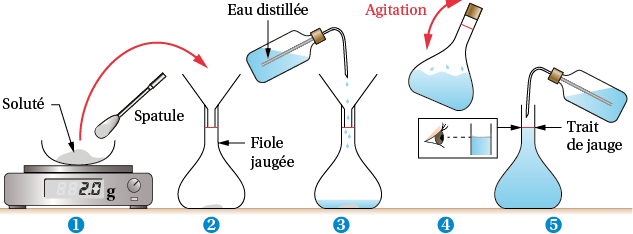
\includegraphics{figures/dissolution}
		\caption{Schéma de la dissolution}
	\end{center}	
\end{figure*}


\newpage
\subsection{Deuxième technique: par dilution}

\etiquette{Contexte et Matériel} 
\begin{itemize}
\item On dispose d'une solution concentrée: \trou{solution mère}. On veut préparer une solution de plus petite concentration: \trou{solution fille}. 
\item On prélève un volume de solution mère auquel on ajoute de l'eau de manière à abaisser la concentration. 
\item On utilise une\trou{ pipette jaugée}, une fiole jaugée et de l'eau distillée
\end{itemize}
\etiquette{Mise en Pratique}
\begin{figure*}[htp!]
	\begin{center}
		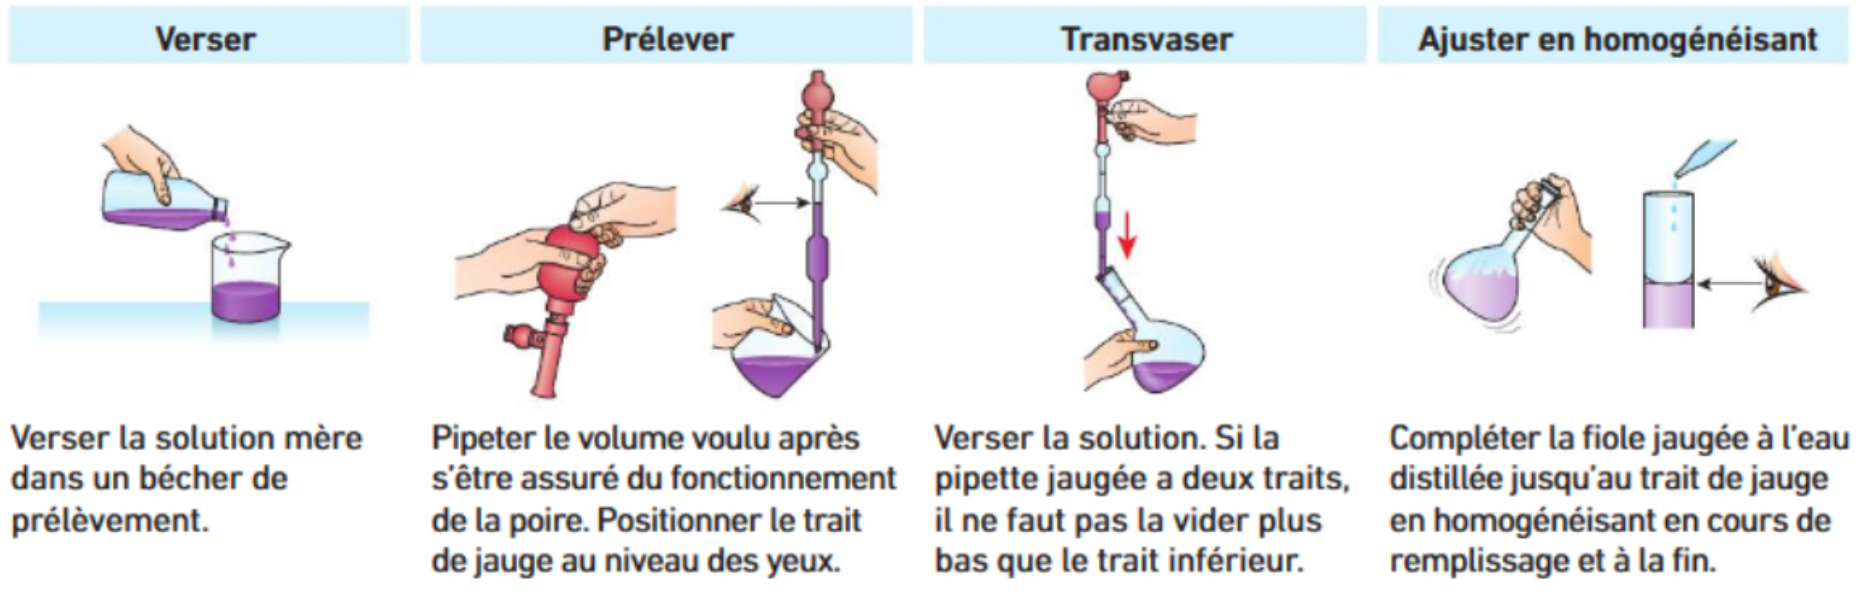
\includegraphics[width=1\textwidth]{figures/dilution}
		\caption{Schéma de la dilution}
	\end{center}	
\end{figure*}

\subsection{Calculs de dilution}

Pour effectuer une dilution, on doit calculer le volume de solution mère à prélever. Cela nous donne aussi le volume de la pipette jaugée à utiliser. Pour faire ce calcul, on utilise le\trou{ facteur de dilution}.
%\paragraph*{Conservation de la matière}
%
%On dispose d'une solution d'eau salée à $C_1= 10$ g/L. On veut préparer $V_2=50$ mL de solution d'eau salée à $C_2= 4,0$ g/L. 
%
%\etiquetterouge{Idée} La quantité de solution présente dans la solution fille de  volume $V_2$ est exactement contenue dans le petit volume \trou{$V_1$ } de solution mère prélevée.
%
%Il y a la même quantité de soluté dans la solution fille de concentration $C_2$ et de volume $V_2$ que dans le prélèvement de solution mère de volume $V_1$ et de concentration $C_1$. Faire un schéma de cette phrase.
%
%On a donc:$$\trou{C_1\times V_1 = C_2\times V_2}$$ Le volume à prélever cherché est $$V_1=\frac{C_2.V_2}{C_1}$$

\blocrouge{Définition}{Le facteur $F$ de dilution est le rapport entre la concentration de la solution mère $C_1$ et la concentration de la solution fille $C_2 < C_1$. C'est aussi le rapport entre le volume de la solution fille et le volume de solution mère à prélever (volume de la pipette)$$\trou{F=\frac{C_1}{C_2}=\frac{V_2}{V_{pipette}}}$$
}

\blocgris{Exemple important}{
On dispose d'une solution d'eau salée à $C_1= 10$ g/L. On veut préparer $V_2=50$ mL de solution d'eau salée à $C_2= 4,0$ g/L. Calculer $V_1$ en utilisant la méthode du facteur de dilution.
\vspace{8cm}}
 
 \etiquette{Exercice} Dissolution et Dilution

On dispose de chlorure de sodium solide ($NaC\ell$). On souhaite
réaliser une solution $S_1$ de volume $V_1=50$ mL et de concentration
$C_1=\SI{1.50e-2}{\mol\per\liter}$. La masse molaire du chlorure de
sodium est 58,5 g/mol.

\begin{enumerate}
    \item Indiquez le protocole expérimental permettant de réaliser la solution $S_1$. On fera un schéma, un calcul et des phrases.
    \item A partir de $S_1$, on prépare une solution $S_2$ de volume $V_2=75,0$ mL et de concentration de $C_2=\SI{5.00e-3}{\mol\per\liter}$. Détailler le protocole expérimantal qui conduit à l'élaboration de $S_2$. On fera la liste du matériel et des schémas clés.
\end{enumerate}

 \section{Transformations chimiques}
 \subsection{C'est quoi une transformation chimique ?}
 Parfois lorsque l'on met en contact deux substances chimiques, elles se transforment en de nouvelles substances.  On parle de transformation chimique. Les substances présentes au début, s'appellent les\trou{ \textbf{réactifs}}. Ils sont consommés au cours de la réaction. Les nouvelles substances qui apparaissent sont appelées \trou{\textbf{produits}}. 

 \subsection{Comment ça s'écrit ?}
 On modélise la transformation par une équation de réaction. \\

\blocgris{Exemple pas à pas}{ 
Le propane ($\mathrm{C_3H_8}$) réagit avec le dioxygène pour donner du dioxyde de carbone et de l'eau. Comment écrire l'équation chimique de cette transformation ?\\
\begin{enumerate}
	\item Faisons la liste des réactifs et des produits.
\\
Initialement les espèces présentes sont les réactifs: $C_3H_8$ et $O_2$. Celles qui aparaissent sont $CO_2$ et $H_2O$	
	
	\item Proposer une écriture de l'équation de le réaction.\\
On commence par écrire:$$C_3H_8 + O_2 \longrightarrow CO_2 + H_2O$$
\item On ajoute des \textbf{coefficients stoechiométriques} pour valider les 2 principes importants (ci-dessous)
 $$\trou{3}\times\boxed{C_3H_8} + \trou{5}\times\boxed{O_2} \longrightarrow \trou{3}\times\boxed{CO_2} + \trou{4}\times\boxed{H_2O}$$\\
 Ce qu'on écrit simplement:
 $$C_3H_8 + ...O_2 \longrightarrow 3CO_2 + ...H_2O$$
\end{enumerate}
}
\paragraph*{Lecture d'une équation chimique} Lorsque 3 moles de propane sont consommées cela consomme aussi 5 moles de $O_2$. La réaction produit alors 3 moles de $CO_2$ et 4 moles d'eau.

\blocrouge{2 Principes importants}{
Une équation chimique est équilibrée si elle vérifie:
\begin{enumerate}
\item La conservation de chaque élément chimique.
\item La conservation de \trou{la charge} (charge de l'ensemble des réactifs = charge de l'ensemble des produits). 
\end{enumerate}
}

 \subsection{Méthode du tableau d'avancement}
Pour décrire quantitativement la transformation chimique, on considère 3 états particuliers:
\begin{enumerate}
	\item L'état initial: les réactifs n'ont pas encore réagi. L'avancement x vaut 0 mol.
	\item L'état intermédaire: la réaction a commencé à se faire mais n'est pas terminée.  $0<x<x_f$
	\item L'état final: Les quantités de matière n'évoluent plus. L'avancement a atteint sa dernière valeur: $x_f$
\end{enumerate}

\blocgris{Exemple pas à pas}{
On fait réagir 1 mol de $H_2$ avec 2 mol d'$O_2$. Le produit obtenu est de l'eau. Cette réaction est \textbf{totale}. On cherche la quantité de matière d'eau que va produire cette réaction.\\
Nou construisons un tableau d'avancement :\\
		\begin{center}
		\begin{tabular}{|l|c|c|c|c|}
\hline 
  \multicolumn{2}{|c!{\protect\makebox[0cm]{:}}}{\textbf{Equation chimique}} &
 \multicolumn{1}{c!{\makebox[0cm]{+}}}{%
      $\mathrm{2H_2(g)}$} &
       \multicolumn{1}{c!{\protect\makebox[0cm]{$\rightarrow$}}}{%
      $\mathrm{O_2(g)}$} &
       \multicolumn{1}{c|}{%
      $\mathrm{2H_2O(g)}$} 
	 
%\tabularnewline
\\
\hline 
Etat du système&
avancement& $\mathrm{n_{H_2}}$ 
&$\mathrm{n_{O_2}}$  
&$\mathrm{n_{H_2O}}$ 

\tabularnewline
\hline 
Etat initial&
$x=0$&.....
&.....
&.....

\tabularnewline
\hline 
Etat intermédiaire&
$x$&$....$
&$....$
&$....$

\tabularnewline
\hline 
Etat final&
$x=x_{f}$&$....$
&$.....$
&$.....$
\tabularnewline
\hline
\end{tabular}
\end{center}
\begin{enumerate}
	\item On relève les quantités matière initiales et on les place à la première ligne du tableau.
	\item A l'état intermédiaire, le contenu des cases est de la forme $n_{initial}-CoeffStoechio\times x$ pour les réactifs et $CoeffStoechio\times x$ pour les produits.
	\item Idem état intermédiaire en remplaçant $x$ par sa valeur particulière $x_f$.
\end{enumerate}

Cela donne 
		\begin{center}
		\begin{tabular}{|l|c|c|c|c|}
\hline 
  \multicolumn{2}{|c!{\protect\makebox[0cm]{:}}}{\textbf{Equation chimique}} &
 \multicolumn{1}{c!{\makebox[0cm]{+}}}{%
      $\mathrm{2H_2(g)}$} &
       \multicolumn{1}{c!{\protect\makebox[0cm]{$\rightarrow$}}}{%
      $\mathrm{O_2(g)}$} &
       \multicolumn{1}{c|}{%
      $\mathrm{2H_2O(g)}$} 
	 
%\tabularnewline
\\
\hline 
Etat du système&
avancement& $\mathrm{n_{H_2}}$ 
&$\mathrm{n_{O_2}}$  
&$\mathrm{n_{H_2O}}$ 

\tabularnewline
\hline 
Etat initial&
$x=0$&1&2&0

\tabularnewline
\hline 
Etat intermédiaire&
$x$&1-2x&2-x&2x
\tabularnewline
\hline 
Etat final&
$x=x_{f}$&$1-2x_f$
&$2-x_f$
&$2x_f$
\tabularnewline
\hline
\end{tabular}
\end{center}
}


Lorsque la réaction est totale, elle continue à se faire jusqu'à ce qu'un des réactifs soit entièrement consommé. 

\blocrouge{A retenir}{

\begin{itemize}
	\item Par définition, le réactif est entièrement consommé à l'état final et s'appelle \textbf{réactif limitant}.
	\item Si la réaction est \textbf{totale} et on a: \\ \boxed{ $$\trou{x_f = x_{max}}$$}.
\end{itemize}
}

Voyons la méthode pour calculer $x_{max}$:

\blocgris{Exemple pas à pas}{
\paragraph*{Hypothèse 1:} le $H_2$ est le réactif limitant 
Alors $1-2x_{max}=0$ et $x_{max}= ... \si{\mole}$\\
\paragraph*{Hypothèse 2:}  $O_2$ est le réactif limitant 
Alors $2-x_{max}=0$ et $x_{max}=$\\
Nous garderons \textbf{toujours la plus petite valeur} de $x_{max}$. \\
Dans notre exemple, on aura donc $x_{max}=.....$ et $H_2$ est le réactif limitant.\\
\paragraph*{Bilan de matière à l'état final}
On remplace $x_f$ par la valeur de $x_{max}$ que l'on vient de calculer dans toutes les cases de l'état final.
On trouve: 

		\begin{center}
		\begin{tabular}{|l|c|c|c|c|}
\hline 
  \multicolumn{2}{|c!{\protect\makebox[0cm]{:}}}{\textbf{Equation chimique}} &
 \multicolumn{1}{c!{\makebox[0cm]{+}}}{%
      $\mathrm{2H_2(g)}$} &
       \multicolumn{1}{c!{\protect\makebox[0cm]{$\rightarrow$}}}{%
      $\mathrm{O_2(g)}$} &
       \multicolumn{1}{c|}{%
      $\mathrm{2H_2O(g)}$} 
	 
%\tabularnewline
\\
\hline 
Etat du système&
avancement& $\mathrm{n_{H_2}}$ 
&$\mathrm{n_{O_2}}$  
&$\mathrm{n_{H_2O}}$ 

\tabularnewline
\hline 
Etat initial&
$x=0$&1&2&0

\tabularnewline
\hline 
Etat intermédiaire&
$x$&1-2x&2-x&2x
\tabularnewline
\hline 
Etat final&
$x=x_{f}=x_{max}= 0,5$&$1-2\times 0,5 = 0$
&$2-0,5=1,5$
&$2\times 0,5=1 $
\tabularnewline
\hline
\end{tabular}
\end{center}
}

A l'aide de la méthode du tableau d'avancement, on prédit qu'à l'état final le système chimique aura la composition suivante:
\begin{itemize}
	\item $\mathrm{n_f(H_2)}=1-2\times0,5=\SI{0}{\mole}$
	\item $\mathrm{n_f(O_2)}=2-0,5=\SI{1.5}{\mole}$
	\item $\mathrm{n_f(H_2O)}=2\times0.5=\SI{1}{\mole}$
\end{itemize}

\paragraph*{Remarques}
\begin{itemize}
	\item Lorsque la réaction n'est pas totale, à l'état final \trou{$x_f < x_{max}$} et au lycée il n'y a pas de méthode générale pour prédire sa valeur. Une réaction non totale est aussi appelée: équilibre chimique et l'état final est l'état d'équilibre (nous étudierons cela dans le prochain chapitre).
	\item En faisant réagir 2 mol de $H_2$ avec 1 mol de $O_2$ on produit 2 mol de $H_2O$ et il ne reste ni $H_2$ ni $O_2$. Cet état initial particulier s'appelle \trou{mélange stoechiométrique}. Il permet de consommer la totalité de tous les réactifs. Il intervient aussi à l'équivalence des titrages.
\end{itemize}

\blocrouge{Mélange Stoechiométrique}{Soit une équation chimique : $$ aA+bB\longrightarrow cC $$ a,b et c sont les coefficients stoechiométriques des espèces chimiques A, B et C. On note $n_A$ la quantité de matière initiale de A et $n_B$ la quantité de matière de B. Le mélange est stoechiométrique si l'égalité suivante est vérifiée:
  $$\frac{n_A}{a}=\frac{n_B}{b}$$ }


\etiquette{Exercice }

Considérons la réaction chimique suivante :
 $$2 A\ell_{(s)} + 3 C\ell_{2(g)} \longrightarrow 2 A\ell C\ell_{3(s)}$$

On mélange \SI{3.0}{mol} d'aluminium avec \SI{4.0}{mol} de dichlore à l'état gazeux .

\begin{enumerate}
    \item Écrire le tableau d'avancement de cette réaction.
    \item Déterminer l'avancement maximal de la réaction.
    \item Calculer les quantités de matière des réactifs et des produits à l'état final.
    \item Identifier le réactif limitant et le réactif en excès.
    \item Calculer la masse de produit.
\end{enumerate}
 \newpage
 
 \etiquetterouge{Important}
 QR Code des documents partagés sur Google Drive
 \begin{center}
	 
\includegraphics[scale=.4]{figures/qrcode_video_1} 	
 \end{center}

 
 \vspace{2cm}
 
 \blocoval{Essentiels}
 {
 \begin{tabular}{l|l}
 A connaître & Techniques  \\
  \hline
Définitions  & Calculer la quantité de matière à partir de la masse \\
        & Calculer la quantité de matière d'un gaz\\
 Masse volumique&Savoir utiliser la formule\\
 &Distinguer $d$ et $\rho$\\       
Concentration massique et molaire& Equation de dilution\\
& Calculs de concentration\\
Dissolution& Protocole \\
& Calcul de la masse de soluté à peser\\
Dilution& Protocole\\
& Calcul du volume de solution mère à prélever\\
Equation chimique& Savoir équilibrer\\
 & Lecture en terme de consommation et production\\
 Tableau d'avancement & Savoir appliquer la méthode\\ 
 &Déterminer $x_{max}$  et l'état final\\
 Mélange stoechiométrique&Justifier qu'un mélange intial est stoechiométrique

\end{tabular}
 }
 
% \setcounter{chapter}{1}
\chapter{Méthodes Physiques d'analyse}
\section{Spectroscopie UV, Visible}
\subsection{Rappels}
On appelle lumière visible les ondes électromagnétiques dont la longueur d'onde $\lambda$ est comprise entre \trou{ 400 nm et 800 nm.}

\subsection{Solution colorée et absorbance}

Certaines espèces en solutions sont colorées (l'ion permanganate, le diiode, etc). Cette couleur est due à l'absorption de certaines radiations. Le \trou{spectre d'aborption} d'une espèce montre quelles sont les radiations absorbées.

\begin{figure*}[htp!]
	\begin{center}
		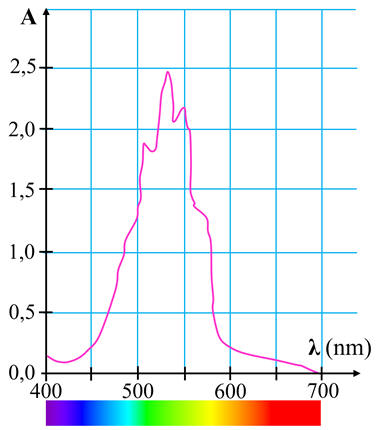
\includegraphics[scale=.4]{figures/spectre_permanganate_2}
		\caption{Spectre d'absorption de l'ion $MnO^{4-}$}
	\end{center}
\end{figure*}

On peut prédire la couleur de la solution en prenant la couleur complémentaire de la couleur la plus absorbée.

Par exemple, l'ion permanganate absorbe dans le jaune-vert. La couleur de la solution de permanganate est violette.


\begin{figure*}[htp!]
	\begin{center}
		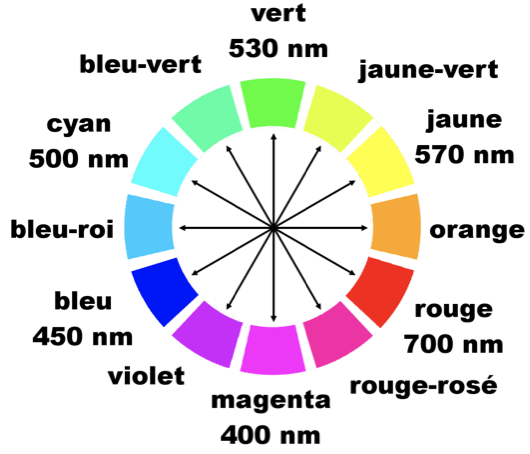
\includegraphics[scale=.6]{figures/cercle_chromatique}
		\caption{Couleurs complémentaires}
	\end{center}
\end{figure*}



\subsection{Spectrophotomètre et Absorbance}
Un spectrophotomètre mesure l'absorbance A d'une solution.

\blocrouge{Définition}{L'absorbance est notée $A$  et qualifie la capacité d'une solution à absorber la lumière (pour une longueur d'onde $\lambda$ fixée). A est un nombre sans unité. }

\paragraph*{Interprétation}

Plus A est grande, plus la solution absorbe et sa coloration est \trou{foncée}.

\blocrouge{Loi de Beer-Lambert}{Pour une solution de concentration $c$ l'absorbance A vaut $$A=k\times c$$ avec $k$ une constante qui dé pend du soluté et de l'épaisseur $\ell$ de la cuve.
De manière plus détaillée, on a $k=\epsilon\times \ell$ avec $\epsilon$ le coefficient d'extinction molaire. 

On peut donc écrire $$A=\trou{ \epsilon\times \ell\times c}$$
}


\etiquetterouge{Important} La loi de Beer-Lambert modélise le relation entre A et c. Ce modèle est bien vérifiée lorsque la concentration est inférieure  à $10^{-2}$ mol/L.

\etiquette{Compléments} L'absorbance se calcule partir de l'intensité lumineuse incidente $I_0$ et l'intensité lumineuse transmise $I_1$ selon $$A = \log{\frac{I_1}{I_0}}$$
\begin{figure*}[htp!]
	\begin{center}
		\includegraphics{figures/fig6}
		\caption{Intensité lumineuse transmise et absorbance}
	\end{center}
\end{figure*}

\subsection{Principe du dosage par étalonnage}

\etiquette{But} On souhaite connaître la concentration d'une solution colorée.

\blocgris{Méthode} 
{
\begin{itemize}
\item Préparer des solutions étalons de concentrations connues par dilution d'une solution contenant l'espèce à doser.
\item Pour chaque solution mesurer l'absorbance.
\item Tracer la droite d'étalonnage, l'absorbance en fonction de la concentration.
\item Mesurer l'absorbance de la solution de concentration inconnue.
\item Utiliser la droite d'étalonnage pour en déduire la concentration cherchée.
\end{itemize}
}

\etiquetterouge{Exercices} 4 p 40 et 17 p 43.
\section{Spectroscopie infrarouge (IR)}
\subsection{Principe}

On constate que certaines radiations électromagnétiques dont les longueurs d'ondes sont dans le domaine de l'infrarouge ($\lambda >800$ nm) sont aborbées par les liaisons chimiques contenues dans une molécule. La valeur de la longueur d'onde absorbée peut être mise en relation avec un type particulier de liaison chimique.

Ces informations se retrouvent sur le spectre IR d'une molécule.

\subsection{Analyse d'un spectre}

Un spectre IR se présente comme ceci :\\
\begin{center}
\includegraphics[scale=0.5]{figures/pentan-2-ol_IR}
\end{center}
En ordonnée, la transmittance, exprimée en pourcentage. 100\% signifie que la radiation n'est pas du tout absorbée, tout est transmis.\\
En abscisse, \trou{le nombre d'onde, noté $\sigma$ et exprimé en $\SI{}{\per\centi\meter}$. Le nombre d'onde est l'inverse de la longueur d'onde, c'est à dire que $\sigma = \dfrac{1}{\lambda}$}\\
Dans le spectre, on observe des bandes d'absorption. Ces bandes correspondent à des liaisons bien particulières, ce qui permet d'identifier dans la molécule des groupes caractéristiques.\\
Pour cela, nous utilisons des tables de référence (cf p 35 de votre livre)

\subsection{Application}
\etiquette{Activité documentaire 2 p 32}
\etiquetterouge{Exercice} 23 p 46

\section{La conductimétrie}
La conductimétrie est basée sur l'étude de la capacité d'une solution à conduire le courant électrique. On ne pourra donc faire une étude conductimétrique qu'avec des solutions électrolytiques, c'est à dire des solutions comportant des ions.
\subsection{La conductance}
Une cellule conductimétrique est constituée de 2 plaques métalliques planes et parallèles de même surface S, distantes de $\ell$, les électrodes.\\
Un conductimètre mesure la résistance de la solution qui se trouve contenue entre les deux plaques.

	\begin{figure*}
	\begin{center}
		\includegraphics[scale=.5]{figures/conductimetre}
	\end{center}
	\end{figure*}

\blocrouge{Définition}{
La conductance est définie comme étant l'inverse de la résistance, c'est à dire : \\
\trou{$G=\dfrac{I}{U}$ avec G en siemens (S) ; I en ampères (A), et U en volts (V)}
}

La résistance est une grandeur représentative de la capacité de la solution à \trou{s'opposer }au passage du courant électrique.\\
La conductance est une grandeur représentative de la capacité de la solution à \trou{conduire }le courant électrique.
\subsection{La conductivité}
La conductance est proportionnelle à l'aire S des électrodes et inversement proportionnelle à la distance $\ell$ les séparant.\\
On a donc $G=\trou{\sigma \dfrac{S}{\ell}}$ ou $\sigma$ est une grandeur notée la conductivité de la solution.

\blocrouge{Définition de la conductivité}{
On a alors $\sigma = \trou{G\dfrac{\ell}{S}}$\\
Avec $\sigma$ \trou{la conductivité en $\SI{}{\siemens\per\meter}$}\\
G \trou{la conductance en S}\\
$\ell$ \trou{la distance entre les plaques en m}\\
S \trou{la surface immergée des électrodes.}
}

Pour une même cellule conductimétrique, la conductivité dépend donc uniquement des caractéristiques de la solution, température, nature et concentration des ions.

\subsection{La loi de Kohlrausch}
Tous les ions n'ont pas la même capacité à conduire le courant électrique. \\
L'influence de la nature de l'ion est caractérisée par la conductivité molaire ionique $\lambda$. %Elle s'exprime en $\SI{}{\siemens\meter\squared\per\mole}$

\blocrouge{Loi de Kolhrausch}{
$\sigma =\trou{\sum\limits_{i=1}^n \lambda_i[X_i]}$\\
Avec $\sigma$ en \trou{$\SI{}{\siemens\per\meter}$}\\
$\lambda$ en \trou{$\SI{}{\siemens\meter\squared\per\mole}$}\\
et [X] en \trou{$\SI{}{\mole\per\meter\cubed}$}\\
\underline{Remarque :} Cette loi n'est valable que pour les solutions de concentration peu élevées (inférieures à $\SI{0,01}{\mole\per\liter}$, c'est à dire $\SI{10}{\mole\per\meter\cubed}$).\\

}
%\vspace{1cm}

\etiquette{Application}
Soit une solution de nitrate d'argent $(Ag^+ + NO_3^-)$ de concentration $\SI{1,0e-2}{\mole\per\liter}$.\\
$Ag^+ = \SI{6,19}{mS.m^2.mol^{-1}} $;
$NO_3^-= \SI{7,14}{mS.m^2.mol^{-1}}$
\begin{enumerate}
\item A partir de la loi de Kolhrausch,  exprimer la conductivité de la solution en fonction des conductivités molaires ioniques des ions présents.
\item Appliquer cette relation pour trouver la valeur de la conductivité de la solution.
\end{enumerate}
\vspace{8cm}

\subsection{Détermination de la concentration d'une solution à partir de sa conductivité}
On obtient une solution, de concentration inconnue c, par dissolution dans l'eau de nitrate de nickel de formule $Ni(NO_3)_2(s)$\\
 On mesure sa conductivité, et l'on trouve $\sigma=\SI{5,00e-2}{\siemens\per\meter}$.\\
 
\begin{enumerate}
\item Ecrire l'équation de dissolution du nitrate de nickel dans l'eau.\\
\trou{$Ni(NO_3)_2(s) \longrightarrow Ni^{2+}(aq) + 2NO_3^-(aq)$}
\item Exprimer, en fonction de c, les concentrations des ions en solution.\\
\trou{$[Ni^{2+}]=c$ et $[NO_3^-]=2c$}
\item Appliquer la loi de Kolhrausch puis exprimer la conductivité dela solution $\sigma$ en fonction des conductivités molaires ioniques des ions présents en solution et de c.\\
\trou{$\sigma=\lambda_{Ni^{2+}}[Ni^{2+}]+\lambda_{NO_3^-}[NO_3^-]$\\
$\sigma = (\lambda_{Ni^{2+}}+2\lambda_{NO_3^-})\times c$\\}
\paragraph*{Remarque :}
\trou{On constate que la conductivité est proportionnelle a la concentration en soluté apporté. $\sigma = k \times c$.}
\item En déduire la valeur de c.\\
\trou{Donc $c=\dfrac{\sigma}{\lambda_{Ni^{2+}}+2\lambda_{NO_3^-}}=\dfrac{\num{5,00e-2}}{\num{10,8e-3}+2\times \num{7,1e-3}}=\SI{2,00}{\mole\per\meter\cubed}=\SI{2,00e-3}{\mole\per\liter}$}
\end{enumerate}


\subsection{Dosage conductimétrique par étalonnage}
\blocgris{Principe d'un dosage par étalonnage}{
Les différentes étapes du dosage par étalonnage conductimétrique: 
\begin{itemize}
\item Préparer des solutions étalons de concentrations connues par dilution d'une solution contenant l'espèce à doser.
\item Pour chaque solution, mesurer la conductance ou la conductivité.
\item Tracer la courbe d'étalonnage : la conductance ou la conductivité en fonction de la concentration.
\item Mesurer la conductance ou la conductivité de la solution de concentration inconnue.
\item Utiliser la droite d'étalonnage pour en déduire la concentration recherchée.
\end{itemize}
}


\etiquetterouge{Important}  La loi de Kolhrausch suppose que la solution ionique est suffisamment diluée ($c<\SI{10e-2}{\mole\per\liter}$) 


\etiquetterouge{Exercices} 6, 7, 14 p 40-42 +  Préparation ECE p 47

\section{Les gaz parfaits}

\subsection{Equation d'état des gaz parfaits}
A l'échelle microscopique, un gaz est modélisé par un ensemble d'entités en mouvement désordonné. Si les interactions entre les entités sont négligeables, un gaz est dit <<parfait>>.  C'est le cas de tous les gaz à basse pression.\\
\blocrouge{Equation d'état des gaz parfaits}{
\trou{$P\times V=n\times R \times T$}\\
Avec P \trou{la pression en Pascal (Pa)}\\
V \trou{le volume en $\SI{}{\meter\cubed}$}\\
n \trou{la quantité de matière en mole (mol)}\\
T \trou{la température en Kelvin (K)}\\
R \trou{la constante des gaz parfait }: $R=\trou{\SI{8,314}{\pascal\meter\cubed\per\mole\per\kelvin}}$
}

On peut donc, à partir de cette équation, calculer une quantité de matière de gaz.

\etiquette{Application}
Sous une pression de $\SI{1,20e5}{\pascal}$, et à une température de $\SI{22}{\celsius}$, un échantillon de gaz supposé parfait occupe un volume égal à $\SI{0,31}{\liter}$. Calculer la quantité de matière correspondante.\\
\trou{$n=\dfrac{PV}{RT}=\SI{1,5e-2}{\mole}$}
\subsection{Volume molaire}
\blocrouge{Définition}{
Le volume molaire des gaz $V_m$ est \trou{le volume occupé par une mole de gaz pour une température et une pression données. Il ne dépend pas de la nature du gaz.\\
on a : $n=\dfrac{V}{V_m}$\\
Avec n la quantité de matière en mol\\
V le volume en L\\
$V_m$ le volume molaire en $\si{\liter\per\mole}$}
}

On a, d'après l'équation d'état des gaz parfaits, $n=\trou{\dfrac{PV}{RT}}$.\\
Or, n est aussi égal à $n=\trou{\dfrac{V}{V_m}}$\\
On en déduit que $V_m=\trou{\dfrac{RT}{P}}$. On retrouve bien que c'est une constante pour une températures et une pression données.


\etiquette{Application}
Calculer le volume molaire à pression standard $\SI{1,01e5}{\pascal}$ et à une température de $\SI{25}{\celsius}$.
\vspace{3cm}

\etiquette{Exercices} 19, 20 et 24 p 44

\etiquetterouge{Synthèse} Résume ici l'essentiel de ce chapitre: ce qu'il faut savoir par coeur et les techniques à connaître.




% \setcounter{chapter}{2}
\chapter{Acides et Bases de Bronsted}
\section{Les acides et bases selon Brönsted}
\subsection{Exemples à connaître}
\begin{minipage}{0.7\textwidth}
Quelques exemples d'acides : \\
\trou{$\rm H_3O^+$  ; $\rm CH_3COOH$ ;  $\rm NH_4^+$ ;  $\rm H_2O$} \\
Quelques exemples de bases :\\
\trou{$\rm HO^-$ ; $\rm NH_3$ ; $\rm CH_3COO^-$  ;  $\rm H_2O$}

\subsection{Définition de Brönsted des acides et des bases}

\blocrouge{Définition}{
Un acide est une espèce capable de \trou{céder un ion Hydrogène $\rm H^+$}\\Exemple : $\rm CH_3COOH=\trou{CH_3COO^-}+H^+$\\
Une base est une espèce capable de \trou{capter un ion Hydrogène $\rm H^+$}\\Exemple : $\rm NH_3+H^+=\trou{NH_4^+}$
}

\subsection{Les couples acide/base}
Reprenons notre exemple : \\
$\rm CH_3COOH=CH_3COO^-+H^+$\\  $\rm CH_3COO^-$ est \trou{une base} puisque c'est une espèce capable de capter un ion Hydrogène. On l'appelle base conjuguée de l'acide $\rm CH_3COOH$ et on forme le couple \trou{$\rm CH_3COOH / \rm CH_3COO^-$}.\\
De façon analogue, $\rm NH_4^+$ est \trou{un acide} car capable de céder un ion Hydrogène. C'est l'acide conjugué du couple \trou{$\rm NH_4^+/NH_3$}.\\
Ecriture générale: les couples acide/base peuvent s'écrire: $\rm AH/A^-$ ou également parfois $\rm BH^+/B$

\end{minipage}
\hfill
\begin{minipage}{0.25\textwidth}

\includegraphics[scale=1]{figures/couplesAB}
\end{minipage}

\etiquette{Ex 4 p 22 questions 1 à 3}

\section{La réaction acide-base}
\subsection{Définition}

C'est une réaction ayant lieu entre \trou{l'acide} d'un couple et la base d'un \trou{autre couple}. C'est un transfert d'ion \trou{Hydrogène} de l'acide vers la base.\\
Exemple : couples $\rm HCl/Cl^-$ et $\rm H_3O^+/H_2O$\\
\trou{$\rm HCl(g)+H_2O(l)\longrightarrow Cl^-(aq)+H_3O^+(aq)$ }

\etiquette{Ex 1 p 20}
\subsection{Activité: Schéma de Lewis et Acidité}
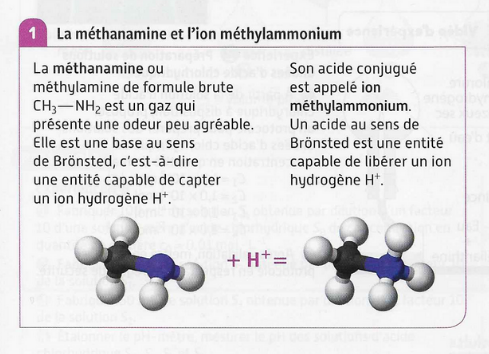
\includegraphics[scale=0.5]{figures/act_1}
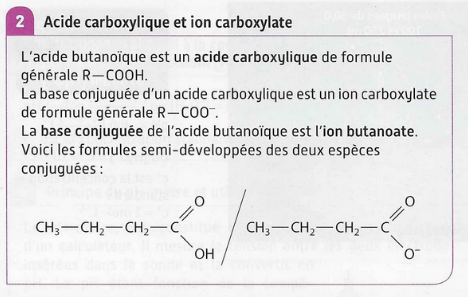
\includegraphics[scale=0.6]{figures/act_2}\\
\paragraph*{Questions}
\begin{enumerate}
	\item Écrire l'équation de la réaction acide-base entre la méthanamine et l'acide butanoïque. Nommer les produits formés.
	\item Établir la configuration électronique des différents atomes présents dans ces deux molécules.
	\item Etablir le schéma de Lewis de chacun de ces atomes.
	\item Représenter le schéma de Lewis de la méthanamine et de l'acide butanoïque.
	\item Identifier les liaisons polarisée avec l'atome d'hydrogène et représenter les éventuelles charges partielles.
	\item Entourer la liaison susceptible de se rompre dans l'acide butanoïque.
	\item Quel est l'élément libéré lors de cette rupture ? Ecrire son schéma de Lewis.
	\item Repérer dans la méthanamine le doublet non liant susceptible de venir combler la lacune électronique de l'ion hydrogène.
	\item Conclusion : En vous appuyant sur le schéma de Lewis justifier le transfert d'ion hydrogène H+ entre l'acide butanoïque et la méthanamine.
\end{enumerate}


\section{Quelques couples acide-base}
\subsection{Les couples des acides carboxyliques}
Un acide carboxylique de formule $RCO_2H$ cède un ion hydrogène $H^+$ pour former un ion carboxylate $RCO_2^-$\\

Ecrire les formules de Lewis de l'acide butanoïque et de l'ion butanoate.
 
\subsection{Les couples de l'eau}
L'eau $H_2O$ appartient à deux couples :
\begin{itemize}
\item Le couple $\trou{H_3O^+}/H_2O$ où elle joue le rôle de la base
\item Le couple $H_2O/\trou{HO^-}$ où elle joue le rôle de l'acide
\end{itemize}
L'eau se comporte soit comme un acide soit comme une base. On dit que l'eau est une espèce \trou{amphotère ou un ampholyte.}
\subsection{Les couples de l'acide carbonique}

L'acide carbonique $H_2CO_3$ est un acide instable qui se forme lors de la dissolution du dioxyde de carbone dans l'eau selon l'équation :
$$CO_{2(g)} + H_2O_{(l)} \leftrightharpoons H_2CO_{3(aq)}$$

La base conjuguée de l'acide carbonique est l'ion hydrogénocarbonate  de formule\trou{   $HCO_3^-$} 

L'ion hydrogénocarbone est un acide, il peut libérer un ion $H^+$ et former un ion carbonate de formule \trou{$CO_3^{2-}$}.

\etiquette{Résumé}

$ H_2CO_3(aq) =  \trou{HCO_3^-} + H^+$\\
$\trou{HCO_3^- }=  CO_3^{2-} +\trou{ H^+}$\\

L'espèce $\trou{HCO_3^-}$ étant à la fois base et acide, c'est, tout comme l'eau, une espèce \trou{amphotère}.\\


\etiquette{Astuce importante} Lorsqu'un exercice parle de dioxyde de carbone dissous, pensez à l'acide carbonique $H_2CO_3$ que l'on écrira très souvent  $CO_2(aq),H_2O(l)$.

\subsection{Les couples des amines}
Les amines sont des molécules azotées, obtenues par remplacement de 1, 2 ou 3 atomes d'hydrogène par 1, 2 ou 3 groupes alkyles.\\
Grâce au\trou{ doublet non liant} porté par l'atome d'azote, les amines sont des espèces capables de capter un ion $H^+$, les amines sont donc des\trou{ bases}.\\


Ecrire les formules de Lewis d'une amine en notant $R_1$, $R_2$ et $R_3$ les groupes liés à l'azote et de l'ion ammonium associé.


\section{Mesure de l'acidité d'une solution}
\subsection{pH}

\blocrouge{Définition}{Le pH d'une solution est un nombre sans unité qui indique l'acidité d'une solution. L'acidité d'une solution est d'autant plus \trou{grande} que le pH est \trou{petit}. Plus la concentration en \trou{ion hydrogène} est grande, plus le pH est petit.

$$\trou{pH = -\log \left(\frac{[H_3O^+]}{c_0}\right)}$$ \trou{avec $c_0 = 1$ mol/L}

A partir de la valeur du pH de la solution, on peut déterminer la concentration des ions hydrogène: $$\trou{[H_3O^+]=10^{-pH}}$$

}

\paragraph*{Remarque} 
\begin{itemize}
 	\item La formule permettant de calculer le pH n'est valable que pour une concentration inférieure à \trou{0,05 mol/L}.

\end{itemize}
\subsection{Exemples et calculs}

\begin{itemize}
\item Le pH d'une solution $S_1$ de concentration en ions oxonium égale à $1,0\cdot 10^{-3}$ mol/L vaut: \trou{$pH = - \log(\frac{[H_3O^+]}{c_0})=-\log(\frac{1,0.10^{-3}\: mol/L}{1\:mol/L}=3,0)$}
\item Le pH d'un soda (considéré comme une solution aqueuse) vaut 2,5. Vérifier que la concentration des ions $H_3O^+$ vaut 3,2 mmol/L.
\end{itemize}

\blocrouge{Exercices à faire} {
\begin{itemize}
	\item 14,15,16 p 24-25 
	\item  20 + prépa ECE p27
\end{itemize}
}
% \setcounter{chapter}{2}
\chapter{Titrages}

\section{Dosage par titrage direct}

\subsection{Définitions}

\blocrouge{Définitions}{
Un \trou{dosage} est une technique expérimentale qui permet de déterminer précisément la \trou{concentration} (ou la quantité de matière) d'une espèce chimique dans une solution.

Un \textbf{dosage par titrage direct} est un dosage qui s'appuie sur une \trou{réaction chimique} appelée \textbf{réaction support du titrage}. Cette réaction doit être :
\begin{itemize}
    \item \trou{rapide}
    \item \trou{totale} (quantitative : le réactif limitant est entièrement consommé)
    \item \trou{univoque} (pas de réaction parasite)
\end{itemize}
}

\blocrouge{Vocabulaire}{
\begin{itemize}
    \item L'\trou{espèce titrée} est l'espèce dont on veut déterminer la concentration. Elle est contenue dans la \trou{prise d'essai} (volume $V_A$ prélevé avec précision).
    \item L'\trou{espèce titrante} est l'espèce de concentration \trou{connue avec précision} ($C_B$). Elle est versée progressivement depuis la \trou{burette}.
\end{itemize}
}

\subsection{Équivalence}

\blocrouge{Définition et relation à l'équivalence}{
L'\textbf{équivalence} d'un titrage est l'état du système pour lequel les réactifs ont été introduits en \trou{proportions stœchiométriques}.

Pour une réaction de la forme : $a\,A + b\,B \rightarrow \text{produits}$

À l'équivalence :
$$\trou{\frac{C_A \cdot V_A}{a} = \frac{C_B \cdot V_{B,\text{éq}}}{b}}$$

$V_{B,\text{éq}}$ est le \textbf{volume équivalent} : volume de solution titrante versé à l'équivalence.
}

\etiquetterouge{Méthode} Pour exploiter un titrage :
\begin{enumerate}
    \item Repérer l'équivalence et lire $V_{B,\text{éq}}$ sur l'axe des abscisses.
    \item Appliquer la relation : $C_A = \dfrac{a \cdot C_B \cdot V_{B,\text{éq}}}{b \cdot V_A}$
\end{enumerate}

\etiquette{Application}

\begin{enumerate}
    \item $V_A = \SI{10.0}{\milli\liter}$ d'une solution d'acide lactique $C_3H_6O_3$ est titrée par une solution de soude $C_B = \SI{1.0e-2}{\mol\per\liter}$. Le volume équivalent est $V_{\text{éq}} = \SI{15.0}{\milli\liter}$.
    \begin{enumerate}
        \item Identifier la solution titrante et la solution titrée.
        \item Écrire la réaction support du titrage.
        \item Calculer la concentration $C_A$ de la solution d'acide lactique.
    \end{enumerate}
    \item $V_B = \SI{10}{\milli\liter}$ d'une solution d'éthanoate de sodium ($\text{Na}^+ + \text{CH}_3\text{COO}^-$) est titrée par une solution d'acide chlorhydrique de concentration $c = \SI{0.024}{\mol\per\liter}$. Le volume équivalent est $V_{\text{éq}} = \SI{8.0}{\milli\liter}$.
    \begin{enumerate}
        \item Identifier titrante et titrée.
        \item Écrire la réaction support.
        \item Calculer la concentration de l'éthanoate de sodium.
    \end{enumerate}
\end{enumerate}

\vspace{5cm}

\section{Titrage pH-métrique}

\subsection{Principe et montage}

Un titrage \trou{pH-métrique} consiste à suivre l'évolution du \trou{pH} de la solution titrée au cours de l'ajout de la solution titrante.

La réaction support est une réaction \trou{acido-basique}.

La \textbf{courbe de titrage} est la courbe : $\text{pH} = f(V_{\text{sol. titrante versée}})$

\etiquette{Protocole} Ajouter la solution titrante :
\begin{itemize}
    \item millilitre par millilitre \trou{loin} de l'équivalence ;
    \item par fractions de \SI{0.5}{\milli\liter} ou moins \trou{au voisinage} de l'équivalence ($V_{\text{éq}} \pm \SI{1}{\milli\liter}$).
\end{itemize}

\subsection{Repérage de l'équivalence}

L'équivalence est repérée par un \trou{saut de pH} (variation brusque du pH). On peut la déterminer par deux méthodes :

\blocrouge{Méthode des tangentes}{
On trace deux tangentes à la courbe, \trou{parallèles} entre elles, de part et d'autre du saut de pH. On trace ensuite la droite \trou{médiane} parallèle à ces deux tangentes. \textbf{L'équivalence} est le point d'intersection de cette médiane avec la courbe.
}

\blocrouge{Méthode de la courbe dérivée}{
On trace la courbe $\dfrac{\Delta \text{pH}}{\Delta V} = f(V)$. \textbf{L'équivalence} correspond au \trou{maximum} de cette courbe dérivée.
}

\url{https://youtu.be/z1l8--2KGpQ}

\section{Titrage colorimétrique}

\blocrouge{Principe}{
Un titrage \trou{colorimétrique} utilise un \textbf{indicateur coloré acido-basique} pour repérer l'équivalence par un \trou{changement de couleur}.

La \textbf{zone de virage} de l'indicateur choisi doit \trou{englober le saut de pH} à l'équivalence.
}

\begin{center}
\begin{tabular}{|l|c|c|}
\hline
\textbf{Indicateur} & \textbf{Zone de virage (pH)} & \textbf{Couleur} \\
\hline
Hélianthine & 3,1 – 4,4 & rouge → jaune \\
BBT & 6,0 – 7,6 & jaune → bleu \\
Phénolphtaléine & 8,2 – 10,0 & incolore → rose \\
\hline
\end{tabular}
\end{center}

\etiquette{Remarque} Le titrage colorimétrique est plus rapide que le titrage pH-métrique mais moins précis. On l'utilise pour une mesure rapide ou pour un titrage préliminaire.

\section{Titrage conductimétrique}

\subsection{Principe}

Un titrage \trou{conductimétrique} consiste à suivre l'évolution de la \trou{conductivité} $\sigma$ (ou de la conductance $G$) de la solution titrée au cours de l'ajout de la solution titrante.

La \textbf{courbe de titrage} est : $\sigma = f(V_{\text{sol. titrante versée}})$

\blocrouge{Remarques importantes}{
\begin{itemize}
    \item \trou{Toutes} les espèces ioniques en solution contribuent à la conductivité (y compris les ions spectateurs).
    \item Pour que la courbe soit linéaire par morceaux, le volume versé doit être \trou{petit} devant le volume initial de solution titrée.
    \item Il n'est pas nécessaire de resserrer les versements au voisinage de l'équivalence.
\end{itemize}
}

\subsection{Repérage de l'équivalence}

\blocrouge{Méthode}{
On trace les deux meilleures \trou{droites} approchant chaque partie du nuage de points (modélisation linéaire). \textbf{L'équivalence} est le point d'intersection de ces deux droites, correspondant au \trou{changement de pente} de la courbe. On lit l'abscisse $V_{B,\text{éq}}$.
}

\url{https://youtu.be/Z3-eOJG3im0}

\etiquetterouge{Exercices}

Dans le livre : Ex 6, 11, 13 p.~62\\
Pour aller plus loin : Ex 22 p.~67 ; Ex 25 p.~69\\
\textbf{Sujets bac} : Asie 2021 J2 Ex1 partie 2 ; Amérique du Nord 2021 J1 Ex B ; Antilles-Guyane 2015 Ex 2 (2\ieme{} partie)\\
Vidéo bilan : \url{https://youtu.be/MSEryl_85Oo}

% \setcounter{chapter}{4}
\chapter{Cinématique}
\section{Généralités}

Le mot cinématique vient du grec kinema qui signifie mouvement. La cinématique étudie les mouvements \trou{indépendamment} de leurs causes à savoir les forces.

\subsection{Nécessité de définir un \trou{référentiel}}

Critiquez la formulation de la question: "Êtes-vous immobile ou en mouvement ?" \\

\trou{Nous sommes immobile par rapport au sol et en mouvement par rapport au Soleil. Il est donc indispensable de définir un solide de référence: un référentiel.}

\blocrouge{Définition}{\trou{Un référentiel est un solide considéré immobile par rapport auquel on étudie le mouvement d'un système.}}

L'objet dont on étudie le mouvement est appelé le \textbf{système}. En général, on étudie un point de ce système, le plus souvent il s'agit du centre de gravité.
\subsection{Trajectoire et Chronophotographie}

\blocrouge{Définition}{L'ensemble des positions successives occupées par un point mobile M au cours du temps s'appelle la trajectoire.\\ En relevant à intervalle de temps régulier, la position du point mobile, on obtient une chronophotographie.}

\etiquette{Exemples}
Représentez l'allure de la chronophotographie dans les cas suivants:
\begin{enumerate}
	\item Une bille que l'on lâche
	\item Une bille en mouvement rectiligne uniforme roulant sur le sol (parfaitement glissant).
	\item Un ballon de basket lors dans lancer franc.
	\item Un point en mouvement circulaire uniforme.
\end{enumerate}
\vspace{6 cm}


\section{Le vecteur vitesse}
Le nombre est bien adapté à la description de certaines grandeurs physiques comme la distance, la température, la concentration molaire... Cependant il n'est pas adapté pour décrire un déplacement, une vitesse ou encore une accélération. 
\subsection{Construction à partir d'une chronophotographie}

Faire les questions 1 et 2 du problème à 1D et du problème à 2D sur la fiche pratique "Comment Exploiter une Chronophotographie"

	\subsection{Projections et coordonnées cartésiennes}
	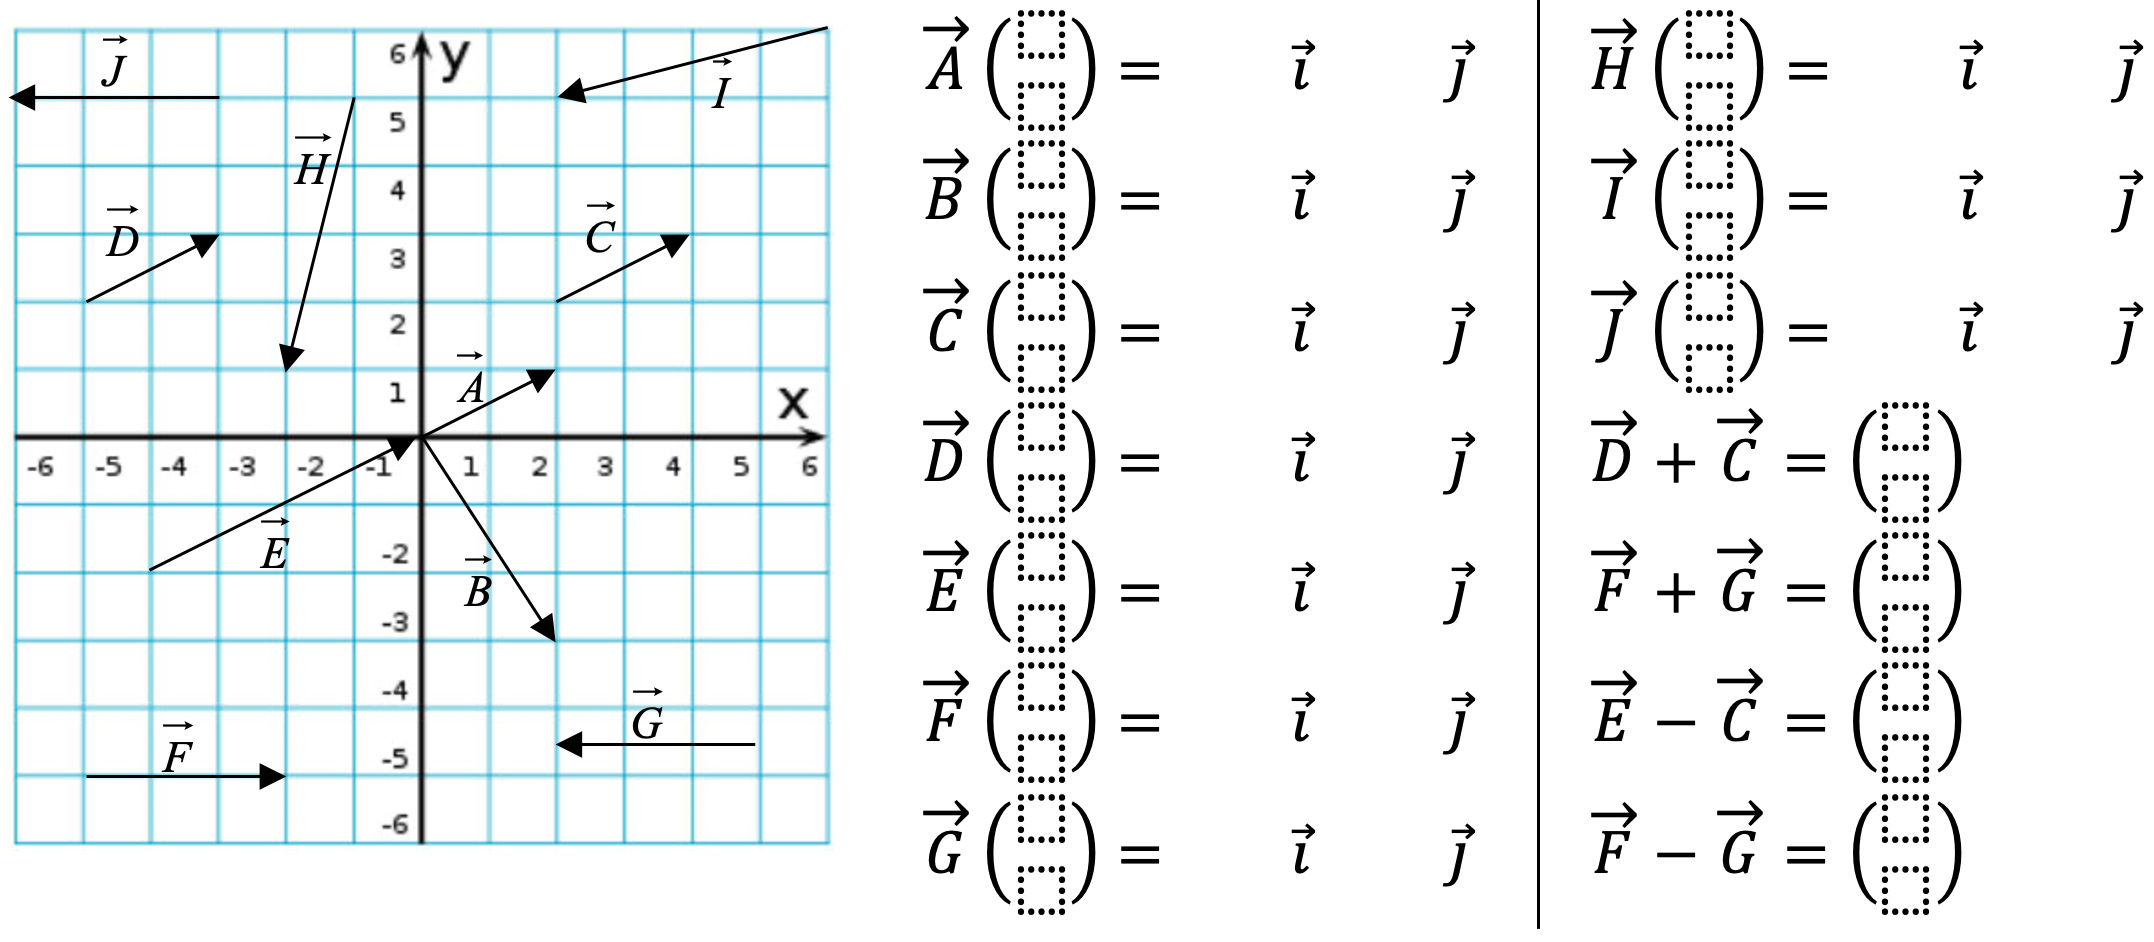
\includegraphics[height=6cm]{figures/cinematique_1}\\
		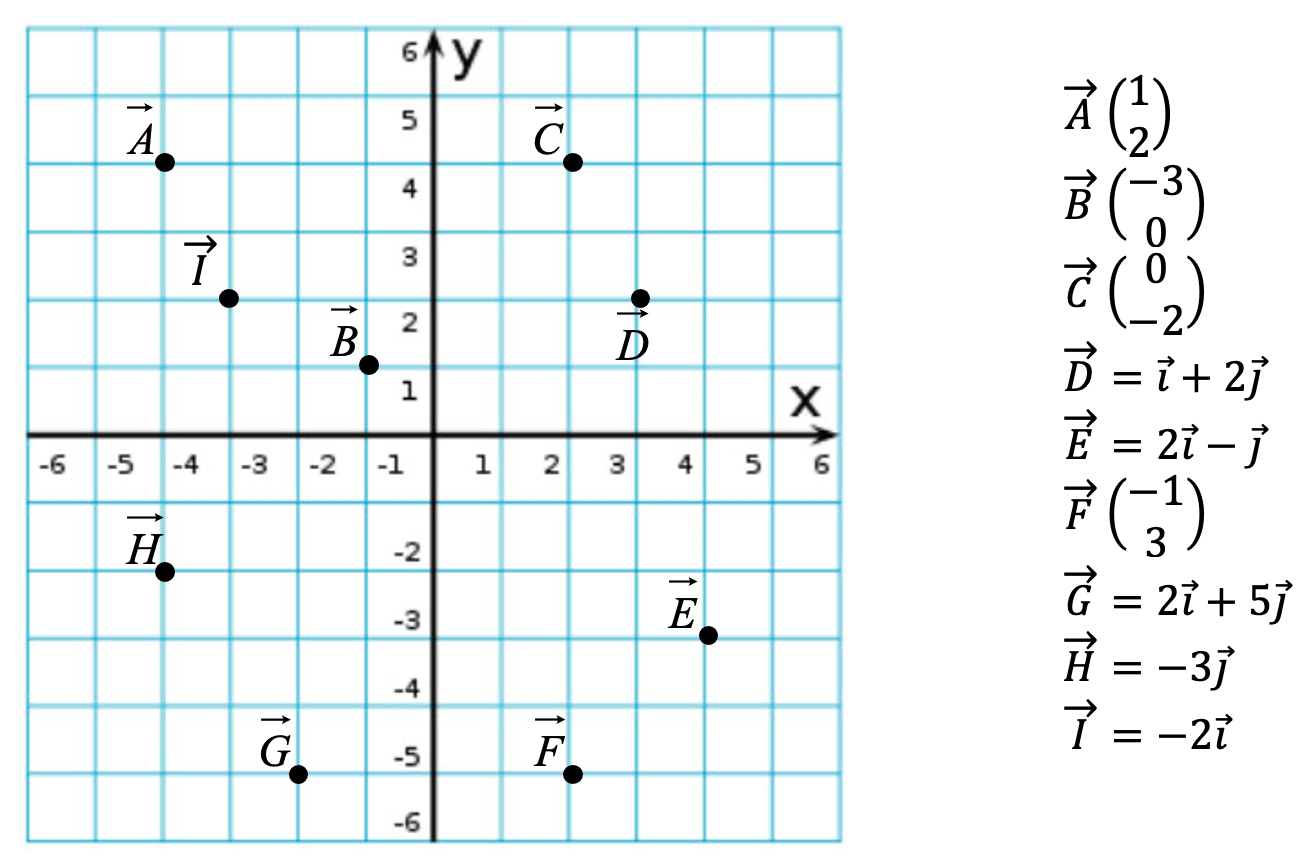
\includegraphics[height=6cm]{figures/cinematique_2}
	\subsection{Position et Vecteur position}
	
Le point M est en mouvement, sa position dépend du temps. C'est pourquoi dans la suite les coordonnées de M sont des fonctions du temps. \\On les note: $x(t)$, $y(t)$ et $z(t)$

Le vecteur position est le vecteur qui relie l'origine du repère et le point mobile M. Il se note: $\overrightarrow{OM(t)}$ ses coordonnées sont les même que le point M. 

\blocrouge{A retenir}{\\
\begin{minipage}{.3\textwidth}
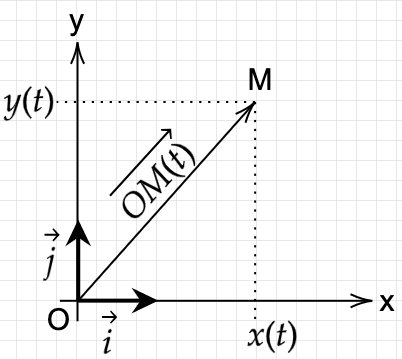
\includegraphics[scale=0.33]{figures/cinematique_3.png}	
\end{minipage}
\hfill
\begin{minipage}{.65\textwidth}
Le vecteur position $\overrightarrow{OM(t)}$  a pour coordonnées: \trou{$
\begin{pmatrix}
	x(t) \\ y(t)
\end{pmatrix}
$}
\\


Une autre écriture est: $\overrightarrow{OM(t)}=$ \trou{$x(t). \vec{i}+y(t). \vec{j}$}
\end{minipage}
}


\paragraph*{Remarques} L'unité de chaque coordonnées est le mètre (m). \\A l'instant initial t=0s, l'abscisse x se notera $x(t=0)$ ou $x(0)$.

\subsection{Dérivation en Math vs Dérivation en Physique}

\etiquette{En math}
En mathématique, on note $f'(x)$ la fonction dérivée de $f(x)$. 
\\ Si $f(x)= 10x^2 -2x + 1$ Alors $f'(x) = 10\times 2.x - 2 + 0 = 20x -2$ 
\\
\etiquette{En Physique}

Au lieu de $f'(x)$ on écrira $\frac{df(x)}{dx}$ ou encore $\frac{df}{dx}$ si il est évident que la variable est $x$.  Donc $$\frac{df}{dx} = 20.x -2$$


Dans ce chapitre, la variable est le temps $t$. Considérons une fonction $g$ de la variable $t$ qui s'écrit: 

\begin{align*}
	g(t) &= -3t^2 + 4t +8\\
	g'(t) &= \trou{- 6t + 4 }\\
	\frac{dg}{dt} &= \trou{-6t+4}
\end{align*}

\etiquette{Exercice}
En cinématique,  on dispose  d'une fonction $x(t) = -\frac{1}{2}t^2 + 3t -7$. Calculer $\frac{dx}{dt}$.

\trou{$frac{dx}{dt}=-t+3$}.


\etiquetterouge{Attention}

Ne pas confondre le $x$ des maths avec le $x(t)$ de la physique !
\newpage
\subsection{Vitesse instantanée et vecteur vitesse}

Vitesse est une expression vague. Il faut parler de \trou{vecteur vitesse} ou bien de \trou{valeur de la vitesse}.

La valeur de la vitesse à un instant précis $t$ s'écrit $v(t)$ et s'exprime en m/s. C'est donc la valeur de la vitesse à la date t.
\\

\blocrouge{Vecteur vitesse $\overrightarrow{v(t)}$ }{\\
\begin{minipage}{.5\textwidth}
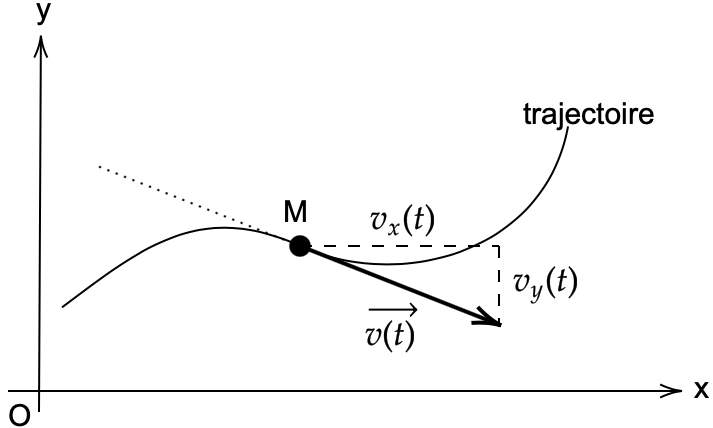
\includegraphics[scale=0.30]{figures/cinematique_4.png}	
\end{minipage}
\hfill
\begin{minipage}{.45\textwidth}
Caractéristiques:
\begin{itemize}
	\item  Direction: Tangente à la trajectoire
	\item Sens: Celui du mouvement
	\item Valeur: la valeur de la vitesse $v(t)$
\end{itemize}
	
\end{minipage}
}


\blocrouge{Définition mathématique du vecteur vitesse}{$$\overrightarrow{v(t)}=\frac{d\overrightarrow{OM(t)}}{dt}$$


Cela signifie que les coordonnées de $\overrightarrow{v(t)}$ s'obtiennent en dérivant les coordonnées  $x(t)$ et $y(t)$ du vecteur position $\overrightarrow{OM(t)}$.

Les coordonnées de $\overrightarrow{v(t)}$ s'écrivent: 


 \[
 \overrightarrow{v(t)} 
\begin{pmatrix}
	v_x(t) = \frac{dx(t)}{dt} \\
		v_y(t) = \frac{dy(t)}{dt}
\end{pmatrix}
\]

}




Pour calculer, les coordonnées de $\vec{v}$ il faudra dériver par rapport au temps les fonctions $x(t)$ $y(t)$ et $x(t)$. 


\subsection{Du vecteur $\vec{v}$ à sa valeur $v$}

\etiquetterouge{Erreur à éviter !}
Il ne faut pas croire qu'un vecteur est un nombre ! Ainsi $\vec{v}$ n'est pas égal à un nombre de m/s.
\\On peut cependant écrire: $$\vec{v}=v_x(t).\vec{i}+v_y(t).\vec{j}$$ il y a bien des vecteurs à gauche est à droite du signe $=$.

La valeur du vecteur $\overrightarrow{v(t)}$ qui s'écrit $v(t)$  est la vitesse instantanée en m/s. Cette valeur s'obtient à partir des coordonnées de $\overrightarrow{v(t)}$.



\blocrouge{Valeur de la vitesse instantanée}{Soit le vecteur vitesse $\overrightarrow{v(t)}$ de coordonnées $v_x(t)$ et $v_y(t)$. La valeur de la vitesse $v(t)$ en m/s vaut:$$v(t)=\trou{\sqrt{v_x(t)^2+v_y(t)^2}}$$

La valeur de la vitesse est aussi appelée norme du vecteur vitesse.
}

\etiquette{Application}

Répondre aux questions de 1 à 7 de la partie Trajectoire et vecteur vitesse de la fiche "Exploiter des équations horaires"

\section{Le vecteur accélération}
\subsection{Construction du vecteur accélération à partir d'une chronophotographie}

\etiquette{Exercice}

Faire la partie Construction du vecteur accélération du problème à 1D et à 2D de la fiche "Comment exploiter une chronophotographie"

\subsection{Calcul du vecteur accélération}
\blocrouge{Définition mathématique du vecteur accélération}{$$\overrightarrow{a(t)}=\frac{d\overrightarrow{v(t)}}{dt}$$


Cela signifie que les coordonnées de $\overrightarrow{a(t)}$ s'obtiennent en dérivant les coordonnées  $v_x(t)$ et $v_y(t)$ du vecteur position $\overrightarrow{v(t)}$.

Les coordonnées de $\overrightarrow{a(t)}$ s'écrivent: 


 \[
 \overrightarrow{a(t)} 
\begin{pmatrix}
	a_x(t) = \trou{\frac{dv_x(t)}{dt}} \\
		a_y(t) = \trou{\frac{dv_y(t)}{dt}}
\end{pmatrix}
\]

}

\paragraph*{Remarques} 
	\begin{itemize}
		\item Le vecteur accélération n'est pas en général dans le sens du mouvement contrairement au vecteur vitesse qui l'est toujours.
		\item On peut obtenir les coordonnées de $\overrightarrow{a(t)}$ en dérivant deux fois les coordonnées de $\overrightarrow{OM(t)}$ Lire point math p 227.
	\end{itemize}

 \etiquetterouge{Erreur à éviter}

\begin{itemize}
\item Le vecteur accélération comme tous les vecteurs n'est JAMAIS égal à un nombre.
		\item Un vecteur accélération non nul ne signifie pas que la valeur de la vitesse augmente (ou diminue). Voir plus loin le cas du mouvement circulaire uniforme.

\end{itemize}
		
\subsection{Calcul de la valeur de l'accélération}
\blocrouge{Valeur de l'accélération }{Soit le vecteur accélération $\overrightarrow{a(t)}$ de coordonnées $a_x(t)$ et $a_y(t)$. La valeur de l'accélération $a(t)$ en mètre par seconde carré vaut:$$a(t)=\sqrt{a_x(t)^2+a_y(t)^2}$$
L'unité de $a(t)$ est: $m/s^2$ ou $m.s^{-2}$

}

\etiquette{Exercice}

Finir la fiche "Exploiter des équations horaires"


\section{Première Synthèse des résultats}
\etiquette{Propriétés des Mouvements Rectilignes à connaître}



\begin{tabular}{|l|l|l|l|}
\hline

  Mouvements&Description & Mathématiques & Exemples\\
\hline  \hline
MRU  & Trajectoire: Droite& $\vec{v}=\trou{\vec{v_0} = \overrightarrow{cste}}$& \trou{Palet de hockey}\\
& Vistesse constante & $\vec{a(t)}=\trou{\vec{0}}$&\\
\hline
MR & Trajectoire: Droite & $\vec{a(t)}=\vec{a_0}= \overrightarrow{cste}$& \trou{-Balle lancée vers le haut}\\
uniformément & $v$ peut augmenter & $\vec{v(t)}=\vec{a_0}\times t+\vec{v_0}\neq \overrightarrow{cste}$& \trou{(phase ascendante)}\\
accéléré & v peut diminuer& &\trou{- Chute libre}\\
\hline

\end{tabular}

\vspace{1cm}
\etiquette{Réactivation}

Pour chacun des exemples du tableau: 
\begin{enumerate}
	\item Représenter une chronophotographie du mouvement.
	\item Représenter quelques vecteurs vitesses de manière réaliste.
	\item Représenter quelques vecteurs accélérations de manière réaliste.
\end{enumerate}


\newpage
\section{Cas des mouvements circulaires}
Dans tout ce qui suit, M est en mouvement circulaire. Sa trajectoire est un cercle de centre O et de rayon R.
\subsection{Base de Frenet}
Pour décrire un mouvement circulaire, on utilise un autre repère: \textbf{la base de Frenet}.
L'utilisation de cette base permet de décrire simplement $\vec{v(t)}$ et $\vec{a(t)}$.

\etiquette{Description}

La base de Frenet a pour origine le point mobile M. De plus, elle possède 2 vecteurs unitaires: $\vec{u_t}$ et $\vec{u_n}$ (parfois aussi noté $\vec{T}$ et $\vec{N}$)
\begin{itemize}
	\item $\vec{u_t}$ est un vecteur  \trou{ tangent } au cercle dans le sens du mouvement de M. 
	\item $\vec{u_n}$ est un vecteur \trou{perpendiculaire} à $\vec{u_t}$ orienté vers l'intérieur du cercle
\end{itemize}

\subsection{Vecteurs dans la base de Frenet}
\blocrouge{Définitions}{


\begin{minipage}{.5\textwidth}
Dans la base de Frenet, pour un mouvement circulaire quelconque les vecteurs vitesse et accélération s'écrivent:
\\
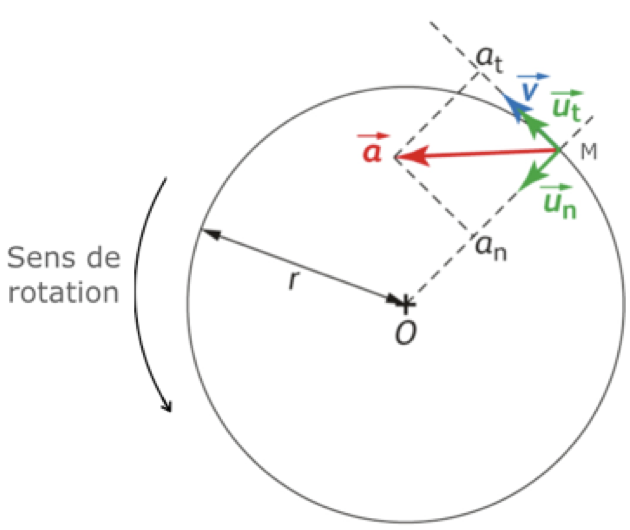
\includegraphics[scale=.65]{figures/cinematique_6}
\\	
\end{minipage}
\begin{minipage}{.45\textwidth}
	$$\vec{v(t)}= v(t). \vec{u_t}$$
		$$\vec{a(t)}= \frac{dv(t)}{dt}. \vec{u_t} + \frac{v^2(t)}{R}.\vec{u_n}$$
		Dans cette base, $\vec{a(t)}$ a pour coordonnées:
	 \[
 \overrightarrow{a(t)} 
\begin{pmatrix}
	a_t(t) = \trou{\frac{dv(t)}{dt}} \\
		a_n(t) = \trou{\frac{v^2(t)}{R}}
\end{pmatrix}
\]

\end{minipage}
}
\paragraph*{Remarque:} Les  vecteurs $\vec{u_t}$ et $\vec{u_n}$ représentés ci-dessus tournent comme M. La base de Frenet: $\vec{u_t}$ et $\vec{u_n}$ est mobile contrairement à la base en coordonnées cartésiennes $\vec{i}$ et $\vec{j}$.
\newpage
\subsection{Cas important du MCU (Mouvement Circulaire Uniforme)}

Dans un mouvement circulaire uniforme, le valeur de la vitesse est constante. 

\etiquetterouge{Attention} Bien que la valeur de la vitesse soit constante, le vecteur vitesse n'est pas constant car sa direction change pendant le mouvement. $\vec{v(t)}\neq\overrightarrow{cst}$.

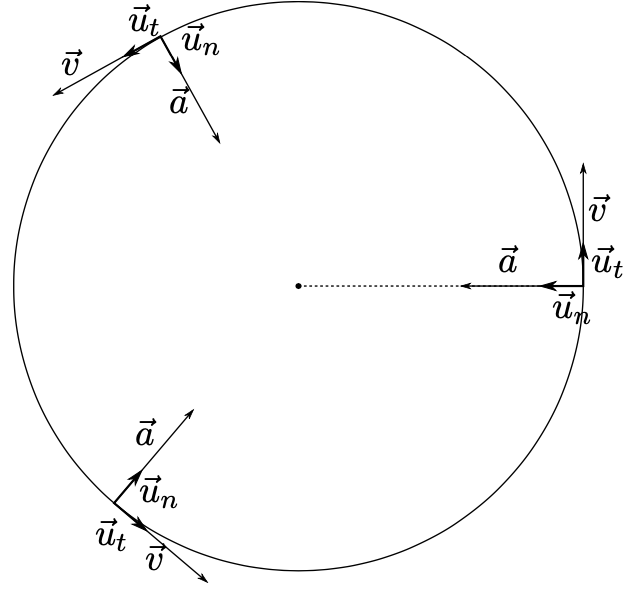
\includegraphics[scale=.5]{figures/cinematique_5}
\blocgris{MCU}{
Dans un MRU, les coordonnées du vecteur accélération s'écrivent simplement:
$$ \overrightarrow{a(t)}=\frac{v^2}{R} .\vec{u_n}$$ 

	 \[
 \overrightarrow{a(t)} 
\begin{pmatrix}
	a_t(t) = \trou{ 0  } \\
		a_n(t) = \frac{v^2}{R} = cste
\end{pmatrix}
\]
}

\newpage
\section{Deuxième Synthèse des résultats}
\etiquette{Cas des mouvements circulaires}


\begin{tabular}{|l|l|l|l|}
\hline

  Mouvements&Description & Mathématiques & Exemples\\
\hline  \hline
MCU & valeur de vitesse constante& $v=cste$& - disque vinyl sur platine\\
    & $\vec{v(t)}$ tourne& $\vec{v(t)}\neq \overrightarrow{cste}$ & -Terre autour du Soleil\\
    & $\vec{a(t)}$ centripète, tourne & $\vec{a}\neq\overrightarrow{cste}$&\\
    & accélération constante&$a=\frac{v^2}{R}=cste$& \\
    \hline
    MC général& -vitesse tangente au cercle& $\vec{v(t)}=v(t).\vec{u_t}$ & -Roue de voiture au\\
    & -vitesse non constante& $v(t)\neq 0$& démarrage\\
    &-accélération vers l'intérieur& $\vec{a(t)}=a_t.\vec{u_t}+a_n.\vec{u_n}$ & \\
    & du cercle & $a_t=\frac{dv(t)}{dt}\neq 0$ & \\
    & & $a_n=\frac{v^2(t)}{R}$&\\
    \hline
    
     
\end{tabular}

\etiquette{Réactivation}

Pour chacun des mouvements du tableau précédent: 
\begin{enumerate}
	\item Représenter une chronophotographie du mouvement.
	\item Représenter quelques vecteurs vitesses de manière réaliste.
	\item Représenter quelques vecteurs accélérations de manière réaliste.
\end{enumerate}

\newpage
\includegraphics[scale=.88]{figures/cinematique_7}

% \setcounter{chapter}{5}
\chapter{Dynamique}
\section{Les Forces}
\subsection{Généralités}

\blocrouge{Définition}{Une force est une action mécanique modélisée par un vecteur $\vec{F}$. Une force est décrite avec la donnée de 4 caractéristiques:

\begin{enumerate}
	\item Point d'application 
	\item Direction
	\item Sens
	\item Valeur
\end{enumerate}}
\subsection{Exemples}
\subsection*{Le poids}

\blocrouge{Définition}{
Le poids $\vec{P}$ d'un système de masse m est la force d'attraction exercée par la Terre sur le système.\\
Caractéristiques :
\begin{itemize}
\item Direction : \trou{verticale}
\item Sens : \trou{vers le bas}
\item Point d'application : \trou{le centre d'inertie du système}
\item Valeur : \trou{$P=m \times g$} avec \\
P \trou{la force en Newton (N)}, m  \trou{la masse en kilogramme (kg)}, et g  \trou{l'intensité de la pesanteur en $\si{\newton\per\kilo\gram}$}
\end{itemize}
}

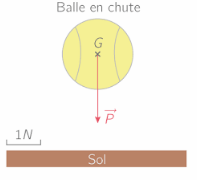
\includegraphics[scale=0.6]{figures/dynamique/poids2}


\subsection*{La réaction d'un support}
\begin{minipage}{0,3\linewidth}
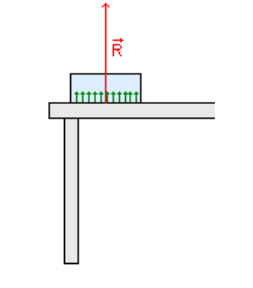
\includegraphics[scale=0.5]{figures/dynamique/reaction}
\end{minipage}
\begin{minipage}{0,7\linewidth}
La force exercée par un support sur un système en contact ($\vec{F}_{support/systeme}$) est encore appelée la \trou{réaction $\vec{R}$} du système.\\
\\
Pour un système immobile ou en mouvement sans frottement sur une surface lisse, les caractéristiques de cette force notée $\vec{R_N}$ pour réaction normale sont : 
\begin{itemize}
\item Point d'application : \trou{centre de la surface en contact}
\item direction :  \trou{perpendiculaire au support}
\item Sens : \trou{orientée du support vers le système.}
\item valeur : \trou{à déterminer selon les cas, notée R.}
\end{itemize}
\end{minipage}


\begin{minipage}{0,3\linewidth}
\includegraphics[scale=0.9]{figures/dynamique/fig1b}
\end{minipage}
\begin{minipage}{0.7\linewidth}

Lorsqu'il y a des frottements, s'ajoute à cette réaction normale $\vec{R_N}$ la réaction tangentielle $\vec{R_T}$, parallèle à la surface de contact et qui modélise les frottements, donc qui s'oppose au mouvement.
\end{minipage}

\blocrouge{A retenir}{ La force $\vec{R}$ exercée par un support sur le système se décompose en général en une somme de 2 vecteurs: $$ \overrightarrow{R}=\trou{\overrightarrow{R_N}}+\trou{\overrightarrow{R_T}}$$ Si les frottements sont négligés  $\overrightarrow{R}=  \overrightarrow{R_N}$ car  $\trou{\overrightarrow{R_T}=\vec{0}}$}

\etiquette{Remarque} Parfois on note $\vec{N}$ le vecteur $\overrightarrow{R_N}$ et $\vec{T}$ le vecteur $\overrightarrow{R_T}$. Attention, rien à voir avec les vecteurs de la base de Frenet.%image réaction normale et réaction tangentielle à trouver
\subsection*{La tension d'un fil}


\begin{minipage}{0,3\linewidth}
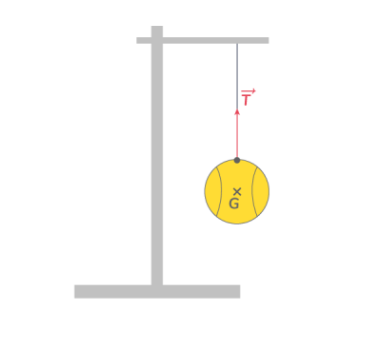
\includegraphics[scale=0.5]{figures/dynamique/tension}
\end{minipage}
\begin{minipage}{0,7\linewidth}
La force exercée par un fil sur un système en contact ($\vec{F}_{fil/systeme}$) est encore appelée la tension $\vec{T}$ d'un fil.\\
\\
Les caractéristiques de cette force sont : 
\begin{itemize}
\item Point d'application : \trou{point d'accroche du système au fil}
\item direction :  \trou{celle du fil}
\item Sens : \trou{orientée du point d'accroche vers le fil.}
\item valeur : \trou{à déterminer selon les cas, notée T.}
\end{itemize}
\end{minipage}

\section{Lois de Newton}
\subsection{Centre de masse}
Les lois de Newton qui vont suivre s'appliquent au centre de masse\footnote{centre de masse = centre d'inertie} G du système. Il s'agit du point où se situe la position\footnote{De manière rigoureuse c'est le barycentre du système. En pratique, il est généralement au centre du système.} moyenne des masses constituant le système. \\
Le centre de masse G est le point du système qui décrit la trajectoire la plus simple.

\etiquette{Ex 11 p 229}

\subsection{Première loi ou principe d'inertie}

Un système est isolé si il n'est soumis à \trou{aucune force} (vue de l'esprit).\\ Un système est pseudo isolé si les forces qu'il subit se compensent c'est à dire: $$\sum \vec{F}= \trou{\vec{F_1} + \vec{F_2}+...} =\vec{0}$$
Subir des forces qui se compensent c'est comme ne pas subir de forces.

\blocrouge{Principe d'inertie}{Dans un référentiel galiléen, si le système est isolé ou pseudo isolé alors son mouvement est \trou{rectiligne uniforme}. Et réciproquement.
\\Formulation mathématique: $$\sum \vec{F}=\trou{\vec{0} } \Leftrightarrow \vec{v} = \trou{\vec{cst}}$$
}

\paragraph*{Remarques} 
Un référentiel est galiléen si le principe d'inertie est parfaitement vérifié dans ce référentiel.\\
Le sol est un référentiel galiléen à condition que l'expérience ne dure pas trop longtemps afin de pouvoir négliger la rotation propre de la Terre\footnote{ Il faut aussi que la masse du système soit faible devant la masse des océans afin de négliger les effets de marées. }

 \etiquette{Réciproque } 
 Si le système est en MRU ou immobile alors d'après le \trou{principe d'inertie} on peut conclure que  les forces se \trou{compensent}.
 
 
 \etiquette{Application 1} Faire l'exercice 1 de la fiche

\subsection{2nde loi de Newton ou relation fondamentale de la dynamique}

\blocrouge{2nde Loi de Newton}{

Dans un référentiel galiléen, l'accélération et les forces subies par le système de masse m sont reliées par:
 $$\sum \vec{F}= \vec{F_1} + \vec{F_2}+... = m\times \vec{a(t)}$$
 
 }
 
 
 \etiquetterouge{Stratégie importante}
 
 Si on connaît les forces appliquées au système, on peut calculer le vecteur $\vec{a}(t)$. Puis, en cherchant des primitives on trouve les coordonnées des vecteurs vitesse et position.
 \vspace{1cm}

\newpage
 \etiquette{Application 2: Détermination du mouvement à partir des forces}
 
Faire l'exercice 2 de la fiche.\\

\subsection{3ème loi de Newton: Principe des actions réciproques}

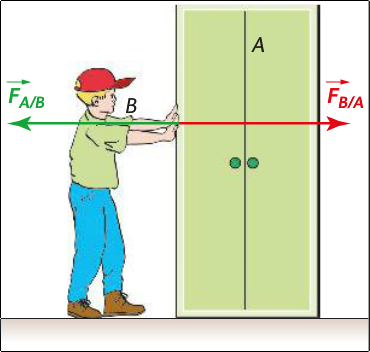
\includegraphics[scale=0.3]{figures/dynamique/fig3}\\
\blocrouge{Enoncé}{A et B sont deux objets en interaction. La force exercée par A sur B est \trou{l'opposée} de la force exercée par B sur A. Ces deux forces ont la même \trou{valeur}, la même \trou{direction}, mais sont de sens \trou{opposés}}
\vspace{1cm}

\etiquette{Capacités Exigibles}
\begin{itemize}
	\item Justifier qualitativement la position du centre de masse d’un système, cette position étant donnée.
	\item Discuter qualitativement du caractère galiléen d’un référentiel donné pour le mouvement étudié.
	\item Utiliser la deuxième loi de Newton dans des situations variées pour en déduire :\\
- le vecteur accélération du centre de masse, les forces appliquées au système étant connues ;\\
- la somme des forces appliquées au système, le mouvement du centre de masse étant connu.
\end{itemize}
 
 \etiquette{Exercices à faire} Voir fiche d'exercices

\includepdf[pages=-]{figures/dynamique/exos_lois_de_newton.pdf}
 
  
% \setcounter{chapter}{6}
\chapter{Mouvement dans un champ uniforme}
\section{Vocabulaire et outils mathématiques}
\subsection{Champ de pesanteur: $\vec{g}$}
\etiquetterouge{Phénomène}  La Terre (comme toutes les grosses masses) crée tout autour d'elle \trou{un champ de pesanteur} que l'on note $\vec{g}$. Lorsqu'une masse $m$ est immergée dans un champ de pesanteur $\vec{g}$ elle subit une force qui vaut $m\times \vec{g}$. Sur Terre, cette force s'appelle aussi le poids et s'écrit: $$\vec{P}=\trou{m.\vec{g}}$$

$\vec{g}$ est vertical, vers le bas et a pour valeur $g=9,8\:m.s^{-2}$.

Lorsqu'en tout point de l'espace $\vec{g}$ garde la même direction, le même sens et la même valeur alors on dit que le champ $\vec{g} $ est \trou{uniforme}.
\paragraph*{Remarque} Dans ce chapitre, le champ de pesanteur est uniforme. 

\subsection{Intégrer une fonction du temps}

\etiquette{Rappel sur la dérivation}

On a vu dans le chapitre précédent, que si on connaît les coordonnées $x(t)$ et $y(t)$ du vecteur position on peut calculer les coordonnées $v_x(t)$ et $v_y(t)$ en utilisant l'opération de \trou{dérivation}.
\\
Par exemple, si $x(t)= -5.t^2 -3t +1$ on  calcule $v_x(t)=\trou{-10t-3}$

\etiquette{Situation} 

Comment faire pour trouver l'expression de $x(t)$ lorsque l'on connaît celle de $v_x(t)$.  On se pose alors la question: "Quelle est la fonction x(t) qui lorsqu'on la dérive donne la fonction $v_x(t)$ ? "\\ On dit que l'on cherche la \trou{primitive de la fonction $v_x(t)$} ou encore que l'on \trou{  intègre  } la fonction $v_x(t)$.

\etiquetterouge{Remarque importante} 

A une fonction $f(t)$ correspond une unique fonction dérivée: $\frac{df(t)}{dt}$ MAIS cette fonction $f(t)$ possède une infinité de primitives. \\ Parmi toutes ces primitives une seule est solution du problème de mécanique étudié\footnote{Pour trouver la "bonne" primitive nous utiliserons des valeurs particulières appelées conditions initiales}.

\etiquetterouge{Primitives à connaître}

\begin{tabular}{l|c}
  $f$ fonction du temps $t$ &Primitive $F(t)$ \\
  \hline \hline 
  $f(t) = 0$ & $F(t)=K$ ; K un réel\\
  \hline
  $f(t) = a$ où a est un réel& $F(t)= a\times t + K$ ; $K$  un réel  \\
  \hline
$f(t)= t$ & $F(t)= \frac{t^2}{2}+ K$ ; K  un réel\\
\hline
$f(t) = a .t + b$ ; a,b deux réels & $F(t)=a.\frac{t^2}{2}+b.t+K$ ; K un réel\\
\hline
\end{tabular}

\etiquette{Application immédiate}
Pour chaque cas, proposer une fonction $x(t)$ qui est une primitive de la fonction $v_x(t)$
\begin{itemize}
	\item $v_x(t) = 5$
	\item $v_x(t)= t$
	\item $v_x(t) = 2t-3$
\end{itemize}


\section{Mouvement dans un champ de pesanteur uniforme}
\subsection{Objectifs}
Nous allons étudier 3 cas: 
\begin{enumerate}
	\item Chute libre sans vitesse initiale.
	\item Chute libre avec une vitesse initiale horizontale.
	\item Chute libre avec une vitesse initiale oblique.
\end{enumerate}

\etiquetterouge{Faites attention à}
	\begin{itemize}
		\item L'enchaînement des étapes qui permettent de passer du bilan des forces aux équations horaires.
		\item Aux conditions initiales, leurs écritures mathématiques et comment elles permettent de déterminer les constantes d'intégration.
	\end{itemize}

\subsection{Chute libre sans vitesse initiale}

\etiquette{Description} 
On lâche à l'instant $\rm t=\SI{0}{\second}$ une bille de masse $\rm m=\SI{100}{\gram}$ d'une hauteur $ \rm h= \SI{5,00}{\meter}$. On notera $\rm \overrightarrow{OM}(t)$ le vecteur position de la bille à chaque instant t.
On note x(t) et y(t) les coordonnées de la bille. 

Les conditions initiales sont $x(0)=0$ ; $y(0)=h=5$ m ; $v_x(0)=v_y(0)=0$ m/s

\includegraphics{figures/dynamique/chute1}


\begin{enumerate}
\item
Faire le bilan des forces exercées sur la bille au cours de la descente.
\item Ecrire la seconde loi de Newton.
\item En déduire les coordonnées du vecteur accélération à l'instant t.
\item En déduire les coordonnées du vecteur vitesse $\overrightarrow{v}(t)$.
\item En déduire les coordonnées du vecteur position $\rm \overrightarrow{OM}(t)$.
\item Le mouvement dépend-il de la masse ? 
\item À quel instant la bille touche-t-elle le sol ? Avec quelle vitesse ?
\end{enumerate}

\subsection{Chute libre avec vitesse initiale horizontale}
\etiquette{Description} On considère une bille M de masse $\rm m=\SI{100}{\gram}$ dont les coordonnées sont notées x(t), y(t) et z(t) à chaque instant. On lance horizontalement à $\rm t=\SI{0}{\second}$ la bille de telle manière que $\rm x(0)=\SI{0}{\meter}$ ; $\rm y(0)=\SI{5}{\meter}$ ; $\rm z(0)=\SI{0}{\meter}$ \\ $\rm v_x(0)=\SI{3}{\meter\per\second}$ ;  $\rm v_y(0)=\SI{0}{\meter\per\second}$ et $\rm v_z(0)=\SI{0}{\meter\per\second}$ 

\includegraphics{figures/dynamique/chute2}


\begin{enumerate}
\item Représentez l'allure de la trajectoire (sans calculs).
\item La vitesse suivant l'horizontale va-t-elle augmenter, diminuer, ou rester constante ?
\item La vitesse suivant la verticale va-t-elle augmenter, diminuer, ou rester constante ?
\item
Faire le bilan des forces exercées sur la bille au cours de la descente.
\item En déduire les coordonnées du vecteur accélération à l'instant t.
\item En déduire les coordonnées du vecteur vitesse $\overrightarrow{v}(t)$.
\item Le mouvement est-il plan ? Justifier.
\item En déduire les coordonnées du vecteur position $\rm \overrightarrow{OM}(t)$.
\item Déterminer l'équation de la trajectoire.
\item À quel instant la bille touche-t-elle le sol ? Avec quelle vitesse ?
Comparer votre résultat à la situation précédente (sans vitesse initiale).
\end{enumerate}

\newpage
\subsection{Le tir parabolique}

\etiquette{Description} On lance une balle selon une direction faisant un angle $\alpha=\SI{60}{\degree}$ avec l'horizontale, avec une vitesse initiale dont la valeur est  $v_0=2\:m /s$. A t=0 s, la balle se situe au niveau du sol, au point O.

\includegraphics{figures/dynamique/chute3}

\begin{enumerate}
\item Faire le bilan des forces exercées sur la bille au cours du mouvement.
\item En déduire les coordonnées du vecteur accélération à l'instant t.
\item En déduire les coordonnées du vecteur vitesse $\overrightarrow{v}(t)$.
\item La vitesse suivant l'horizontale va-t-elle augmenter, diminuer, ou rester constante ? Faire le lien avec le bilan des forces.
\item La vitesse suivant la verticale va-t-elle augmenter, diminuer, ou rester constante ? Faire le lien avec le bilan des forces.
\item En déduire les coordonnées du vecteur position $\rm \overrightarrow{OM}(t)$.
\item Le mouvement est-il plan ? Justifier.
\item Déterminer l'équation de la trajectoire 
\item Déterminer l'abscisse du point d'impact lorsque la balle touche le sol.
\end{enumerate}

\blocrouge{Travail personnel}{
\begin{itemize}
	\item Refaire régulièrement les exemples précédents (faire ses gammes...)
	\item Ex 13 p 252 pour projeter $\vec{v_0}$
	\item Revoir les techniques:  10  ,18 et 28 p 250 et suivantes (calculs classiques)
	\item Préparer le contrôle: 30 p 255
	\item Sujet type bac: Métropole juin 2021 sujet 2 Exercice A question 1 à 5
	\item Sujet bac: Métropole SI 2022 septembre Jour 1 "Etude d'une frappe au football"
	\item Sujet bac: Asie 2021 jour 2 "Water bottle flip"
\end{itemize}}
\newpage
\section{Aspect énergétique}
\subsection{Rappels}
\blocgris{Formules à connaître}{
\begin{itemize}
	\item Energie potentielle de pesanteur: $$Ep=\trou{mgz}$$ \\ $z$ est l'altitude\footnote{On suppose que l'on dispose d'un axe (Oz) verticale orientée positivement vers le O qui permet de repérer l'altitude du système} en mètre du système.
	\item Energie cinétique:$$Ec=\trou{\frac{1}{2}mv^2}$$\\ $v$ la vitesse du système en m/s. 
	\item Energie mécanique:$$Em=\trou{Ec+Ep}$$\\ Les énergies Ep, Ec et Em s'expriment en joules dont le symbole est J. C'est l'unité légale de mesure de l'énergie.
\end{itemize}
}

\blocrouge{Conservation de l'Em}{Si le système n'est soumis qu'à des forces conservatives (comme le poids ou la force électrique) alors son énergie mécanique reste constante. Cela signifie que pour deux instants $t_1$ et $t_2$ on a: $$Em(t_1) = Em(t_2)$$ } 

\paragraph*{Remarque} Les forces de frottements ne sont pas des forces conservatives. Si un système subit des frottements alors \trou{son énergie mécanique sera décroissante au cours du temps}.
\subsection{Etude énergétique d'une chute libre}
On se place dans le cas d'une balle lâchée (sans vitesse initiale)  d'une hauteur  $h=5$ m. A l'instant $t_1=0$ s, la balle est lâchée et à l'instant $t_2$ elle touche le sol.

\etiquetterouge{Objectif} 

Nous allons faire un bilan d'énergie mécanique entre l'instant initial $t_1$ et l'instant $t_2$ où elle atteint le sol. Nous en déduirons la vitesse de la balle à l'instant $t_2$ (moment de l'impact au sol).

\etiquette{Travail}

\begin{enumerate}
\item Rappeler l'expression de la vitesse de la balle au moment où elle touche le sol.
\item Calculer à $t_1$=0 s l'énergie cinétique et potentielle du système. En déduire la valeur initiale de l'énergie mécanique.
\item A l'instant $t_2$, donner l'expression littérale de l'énergie cinétique ? Que vaut l'énergie potentielle à cet instant ?
\item En utilisant la conservation de l'énergie mécanique et les questions précédentes déduire l'expression littérale de la vitesse de la balle à l'instant $t_2$. Faire l'application numérique.
\end{enumerate}

\blocrouge{Travail personnel}{
\begin{itemize}
	\item Ex 1 p 248  et 21 p 253 (énergie mécanique)
	\item Sujet BAC: 2021 Métropole septembre Exercice C: Cesta Punta partie 2
	\item Exercice A: Saut à l'élastique: \url{https://www.labolycee.org/sujets-2-bac-metropole-juin-2021}
	\item Travail de la force électrique BAC 2022 \url{https://www.labolycee.org/impression-3d-dobjets-metalliques}
\end{itemize}
}


\section{Mouvement dans un champ électrique uniforme}
\subsection{Charge électrique $q$}
Certaines particules possèdent une charge électrique que l'on note $q$ et qui se mesure en \trou{coulomb noté: C}.
La plus petite charge électrique s'appelle \trou{la charge élémentaire}, c'est aussi la charge d'un proton. Elle se note $e$ et vaut $$e=\trou{\SI{1.6e-19}{\coulomb}}$$
Par exemple:
\begin{itemize}
	\item la charge de l'électron vaut: $q= -\SI{1.6e-19}{\coulomb}$.  
	\item La charge d'un ion $Cu^{2+}$ vaut $q = 2 \times e = \SI{3.2e-19}{\coulomb}$

\end{itemize}

\etiquetterouge{Phénomène} 
Toute charge électrique crée autour d'elle un champ électrique: $\vec{E}$. Ce champ est représenté par un vecteur dont la valeur s'exprime en \trou{V/m}.


\vspace{1cm}

\includegraphics[width=4cm]{figures/dynamique/chargemoins.png}
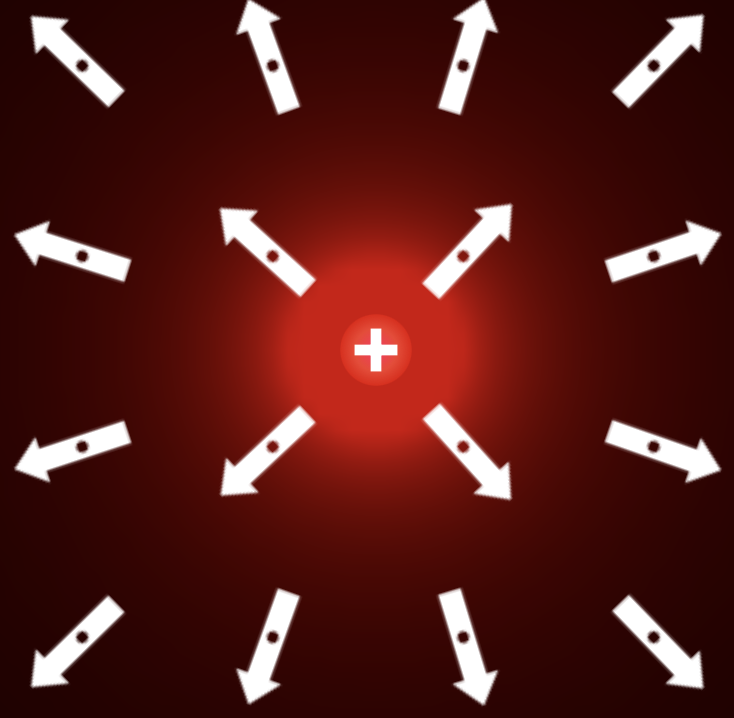
\includegraphics[width=4cm]{figures/dynamique/chargeplus.png}
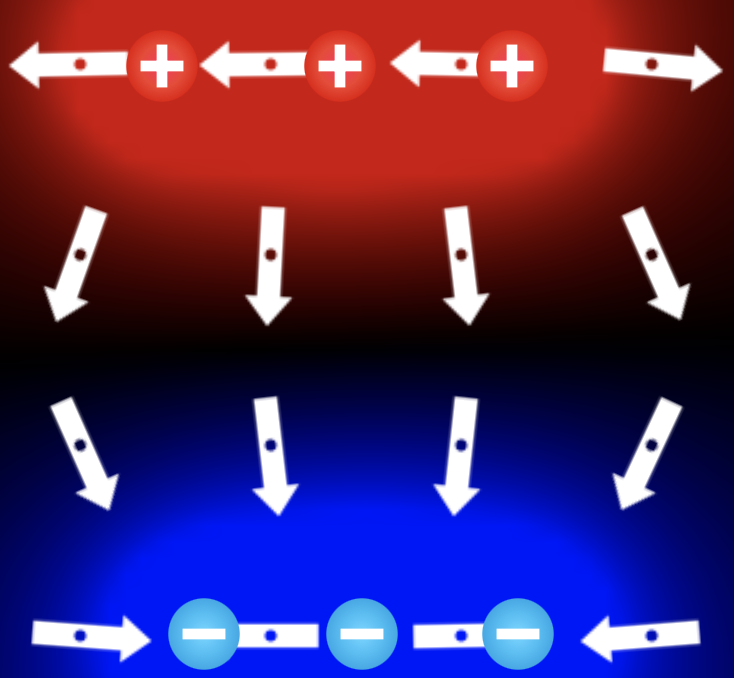
\includegraphics[width=4cm]{figures/dynamique/champ_plaques.png}

\subsection{Champ électrique à l'intérieur de deux plaques chargées}


\etiquette{Situation} On soumet deux plaques métalliques séparées d'une distance $d$ à une tension électrique U imposée par un générateur. Entre ces deux plaques apparaît un champ électrique $\vec{E}$.

A la manière du champ de pesanteur $\vec{g}$, le champ électrique est uniforme (dans la zone entre les plaques) car ses caractéristiques restent les mêmes en tout points. 

\etiquette{Schéma}

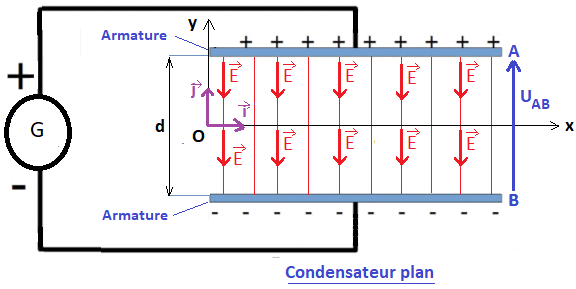
\includegraphics[width=12cm]{figures/dynamique/champ_plaques_2.png}

\blocrouge{Caractéristiques de $\vec{E}$}{
\begin{itemize}
	\item Direction: $\vec{E}$ est  perpendiculaire aux plaques
	\item Sens: orienté de la plaque + vers la plaque -
	\item Valeur: $$E=\trou{\frac{U_{AB}}{d}}$$ Avec $U_{AB}=V_A-V_B$ 
\end{itemize}
E en V/m ; $U_{AB}$ en V et d en m 
}
\etiquette{Calcul de l'intensité du champ électrique}

Le générateur applique une tension de 500 V. Les plaques sont distantes de 5 cm. Calculer la valeur du champ électrique E.







\subsection{Force électrique }

\etiquetterouge{Phénomène} Lorsqu'une charge $q$ est plongée dans un champ électrique $\vec{E}$ elle subit une force $\vec{F}$ qui s'écrit$$\vec{F} = \trou{q\times \vec{E}}$$

\textbf{Attention} Si $q>0$ la force et le champ électrique sont de même sens mais si $q<0$ la force est de sens opposé à $\vec{E}$.
\etiquette{Représentation de $\vec{F}$}

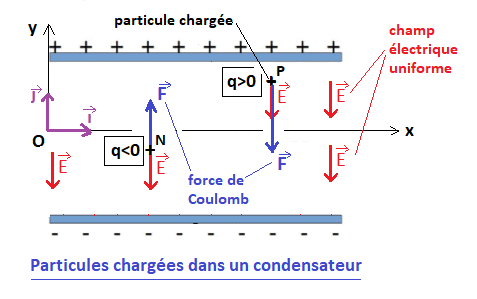
\includegraphics[scale=0.7]{figures/dynamique/force_electrique}

Simulation: \url{https://dlatreyte.github.io/terminales-pc/chap-8/5-mouvement-champ-electrique/}
\etiquette{Application immédiate }
\begin{enumerate}
	\item Représenter, sur les schémas ci-dessous, qualitativement, les charges sur les plaques ou la trajectoire de la particule q.
	\item Sur chaque schéma, représenter $\vec{F}$ et $\vec{E}$

\end{enumerate}

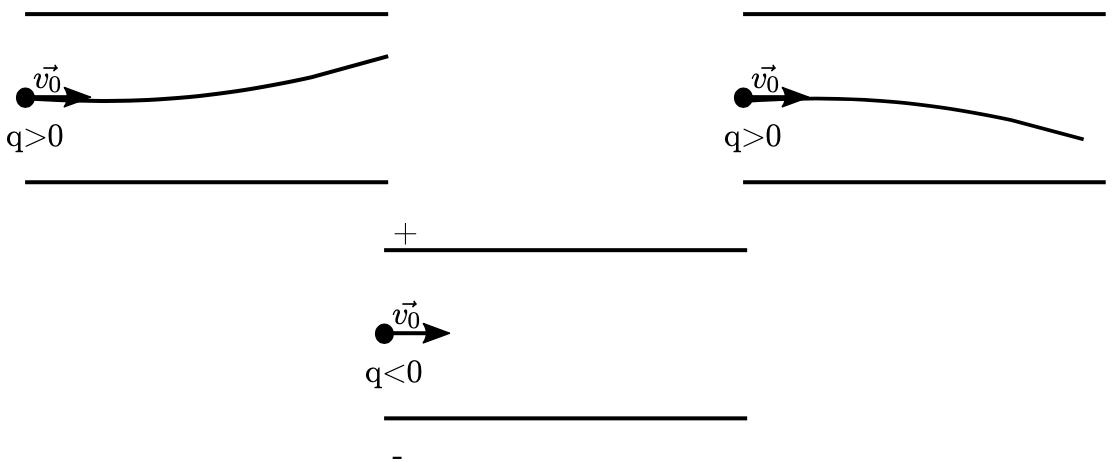
\includegraphics[width=0.8\textwidth]{figures/dynamique/etude_cas}
\newpage
\etiquette{Exercice classique 1}

\begin{minipage}{.50\textwidth}
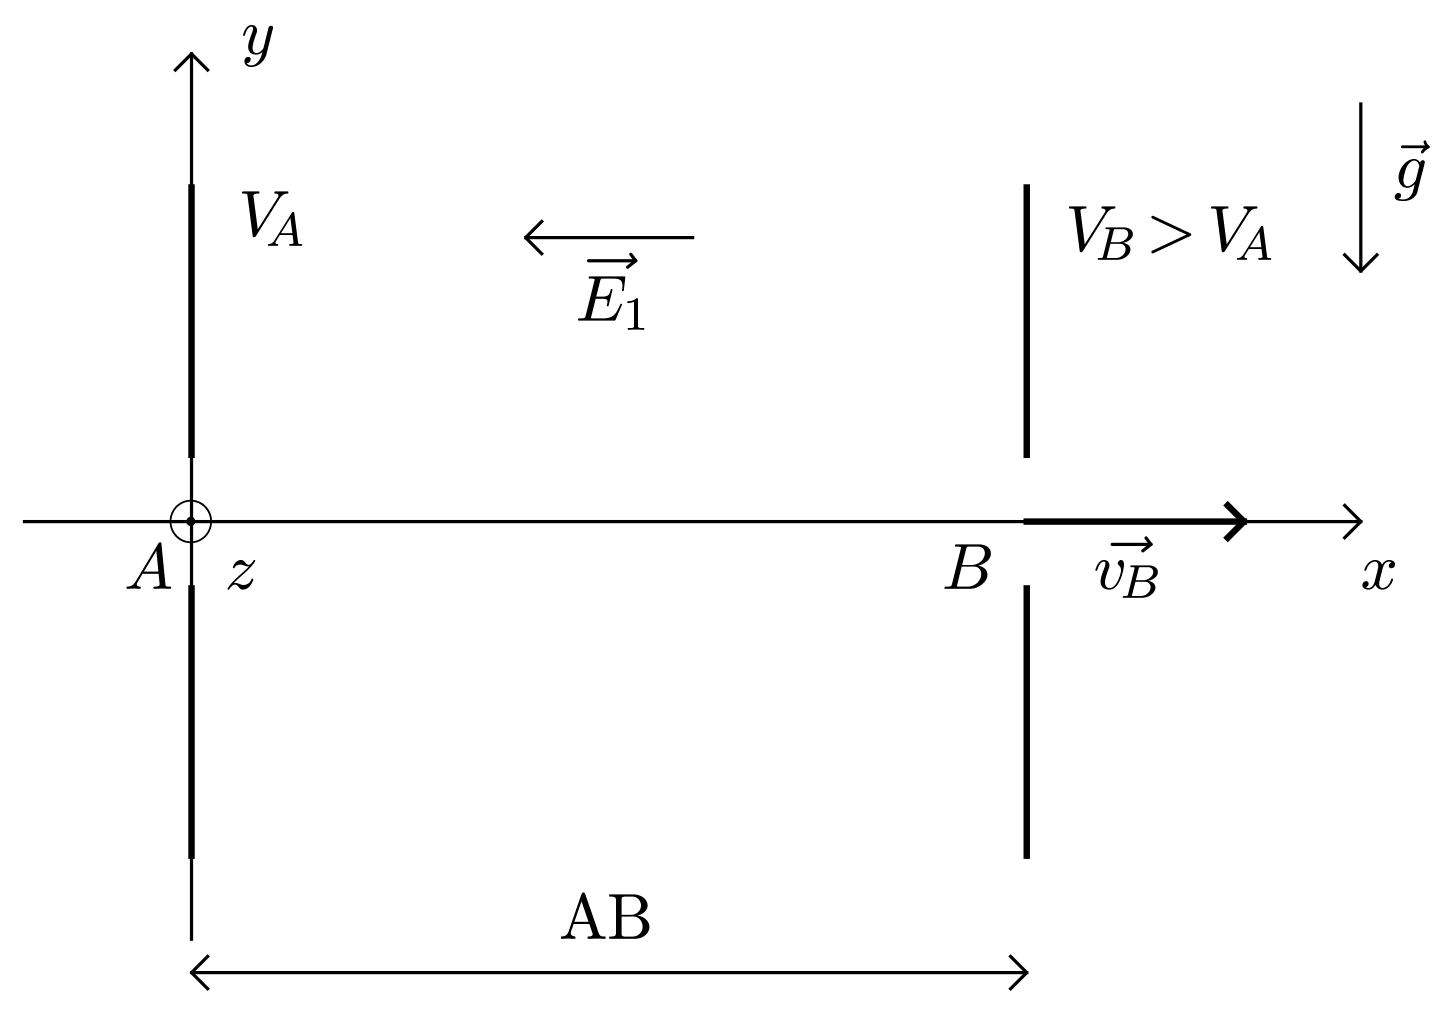
\includegraphics[width=1\textwidth]{figures/dynamique/Chap-8-5-5}  
\end{minipage}
\hfill
\begin{minipage}{.45\textwidth}
Un électron est produit avec une vitesse nulle au point A  entrée d'une zone de l'espace où règne un champ électrique $\vec{E}_{1}$ créé par deux armatures conductrices planes parallèles distantes de AB et le champ de pesanteur $\vec{g}$. On Cherche à déterminer les équations horaires du mouvement de l'électron et plus particulièrement sa vitesse $\vec{v}_{B}$  au point B.\\ \textbf{Données}\
e=\SI{1,6e-19}{C} \\  $m_e$= \SI{9,11e-31}{kg} ; AB= 3 cm ; $E_1$= \SI{6,0e4}{V/m}
\end{minipage}
\paragraph*{Calcul de $v_B$ à partir de la seconde loi de Newton}
\begin{enumerate}
	\item Déterminer les interactions auxquelles est soumis l'électron. 
	\item Ecrire la seconde loi de Newton.
	\item Calculer la valeur de la force électrique puis celle du poids. En déduire que l'on peut négliger dans la suite le poids.
	\item Déterminer les coordonnées du vecteur accélération, vitesse et position. 
	\item Déterminer la valeur de la vitesse en B.
\end{enumerate}


\etiquette{Exercice classique 2}

\begin{minipage}{.50\textwidth}
  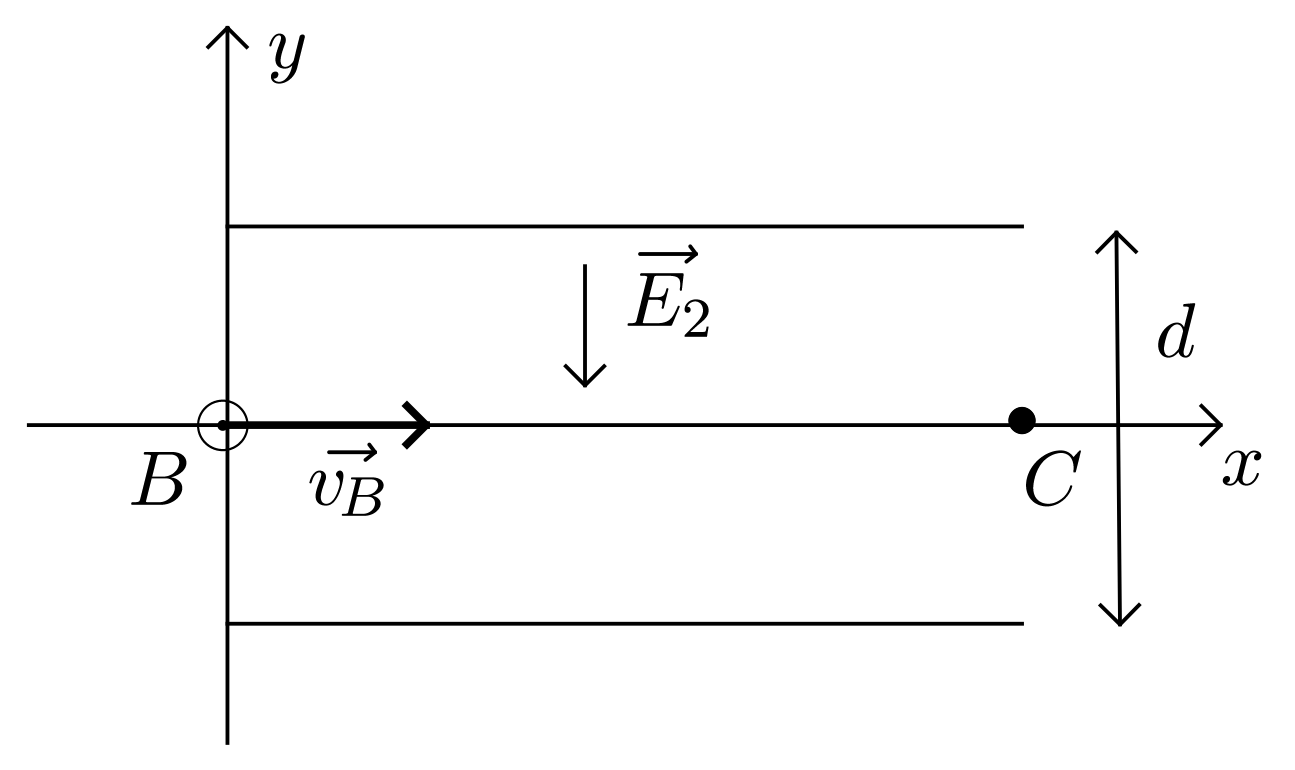
\includegraphics[width=.9\textwidth]{figures/dynamique/Chap-8-5-9}
\end{minipage}
\hfill
\begin{minipage}{.45\textwidth}
  L'électron entre maintenant dans une nouvelle zone dans laquelle règne un champ électrique $\vec{E_2}$ avec la vitesse $\vec{v_B}$ déterminée dans la section précédente.
  A t=0 l'électron est en B.
  
  \textbf{Données}\
BC=6,0 cm ; d= 3 cm ; $E_2$= \SI{1,0e14}{V/m}
\end{minipage}

\begin{enumerate}
	\item Appliquer la seconde loi de Newton et déterminer les coordonnées des vecteurs: accélération, vitesse et position en tenant compte des conditions initiales.
	\item Etablir l'équation de la trajectoire lorsque l'électron est soumis à $\vec{E_2}$.
	\item Déterminer les expressions des coordonnées du point de sortie de l'électron.
	\item Quel  est le mouvement de l'électron lorsqu'il a quitté les deux zones dans lesquelles règnent les champs électriques $\vec{E_1}$  et $\vec{E_2}$ ?
\end{enumerate}

\blocrouge{Travail personnel}{
\begin{itemize}
	\item Ex 11 et 19 p 251 et suivantes 
	\item 33, 34 p 256-257
\end{itemize}

 }
%
%\subsection{Etude du Mouvement d'une charge $q$ dans un $\vec{E}$}
%
%\begin{enumerate}
%\item
%Représenter sur la figure 1 le champ électrique au point O\\
%
%\begin{figure}[htp!]
%\begin{center}
%%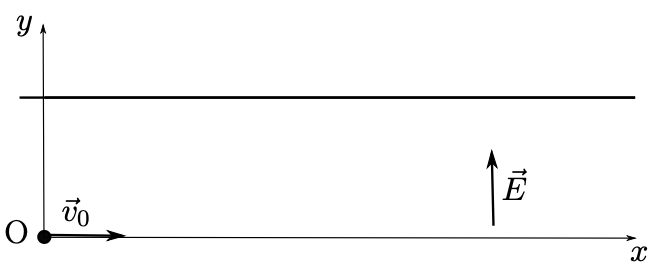
\includegraphics[scale=0.6]{figures/dynamique/fig_exo.png}	
%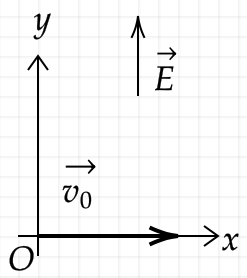
\includegraphics[scale=0.4]{figures/dynamique/mouvement_charge_electrique.png}	
%\end{center}
%\caption{Mouvement d'un électron dans un champ électrique uniforme}
%\end{figure}
%\end{enumerate}
%
%Un électron arrive au point O avec une vitesse initiale $\vec{v}_0$.
%
%\begin{enumerate}
%\stepcounter{enumi}
%\item Exprimer la force $\vec F$ subie par l'électron soumis au champ $\vec E$.
%\item Représenter qualitativement cette force sur la figure 1.
%\item Représenter sur la figure 1  l'allure de la trajectoire de l'électron (sans calculs).
%\item Appliquer la deuxième loi de Newton à l'électron sachant que le poids est une force négligeable devant $\vec F$.
%\item En déduire les coordonnées du vecteur accélération $\vec a$ à un instant t.
%\item En déduire les coordonnées du vecteur vitesse $\vec v$ à un instant t.
%\item En déduire les coordonnées du vecteur position $\vec{OM}$ à un instant t.
%\item Déterminer l'équation de la trajectoire.
%\end{enumerate}
%
%\etiquettebleue{Application numérique} Un faisceau d'ions oxyde $O^{2-}$ est envoyé dans un condensateur plan de longueur $L=\SI{10}{\centi\meter}$ où règne un champ électrique de valeur $E=\SI{100}{\kilo\volt\per\meter}$.\\
%La valeur initiale de la vitesse de chaque ion est $v_0=\SI{5,0e5}{\meter\per\second}$.\\
%Déterminer l'ordonnée de sortie des ions selon qu'ils appartiennent à l'isotope 16 ou à l'isotope 18 de l'oxygène, de masses respectives $m_{16}=\SI{2,66e-26}{\kilo\gram}$ et $m_{18}=\SI{2,99e-26}{\kilo\gram}$.


% \setcounter{chapter}{6}
\chapter{Energies en mécanique}

\section{Travail d'une force}
\subsection{Cas général}

\blocrouge{Définition}{On considère une force $\vec{F}$ dont le point d'application se déplace de A vers B. Le déplacement est représenté par le vecteur $\vec{AB}$. L'énergie transférée au système par la force $\vec{F}$ pendant le déplacement $\vec{AB}$ s'appelle le travail de $\vec{F}$ il a pour expression: $$W(\vec{F}) = \trou{\vec{F}\cdot \vec{AB}} = F \times AB \times \trou{\cos(\alpha)}$$
Unités: W en J ; F en N ; AB en m
}

\etiquetterouge{Cas particuliers importants}
\begin{itemize}
	\item Si $\vec{F}$ est \trou{perpendiculaire} au déplacement alors $W(\vec{F})=0$
	\item Si $\vec{F}$ a même direction et \trou{même sens} que le déplacement $\vec{AB}$ alors $W(\vec{F})=F.AB>0$. La force aide au déplacement, le travail est \trou{moteur}.
	\item Si $\vec{F}$ a même direction et sens opposé au déplacement $\vec{AB}$ alors $W(\vec{F})=\trou{ - F.AB<0}$. La force résiste au déplacement, le travail est \trou{résistant}.
\end{itemize}

\etiquette{Exemples} Rédiger un exemple pour chacune des 3 situations. \vspace{5cm}

\subsection{Cas particuliers importants }
\etiquette{Vocabulaire} Qu'est-ce qu'une \textbf{force conservative } ?\\
\begin{itemize}
	\item Une force est conservative si son travail entre A et B ne dépend pas du chemin suivi pour aller de A à B. 
	\item Le poids et la force électrique sont des forces conservatives. 
\end{itemize}


Ainsi pour calculer le travail du poids on a uniquement besoin de la différence d'altitude entre A et B.

\blocrouge{Travail du poids}{

 Soit $h$ la différence d'altitude (dénivelé) entre A et B. On a $h=|z_A-z_B|$
\begin{itemize}
	\item Si le système descend en se déplaçant de A vers B: $W(\vec{P})=\trou{+mgh}$
		\item Si le système monte en se déplaçant de A vers B: $W(\vec{P})=\trou{-mgh}$ 
\end{itemize}

 Ce qui s'écrit de manière plus générale: $$W_{A\rightarrow B}(\vec{P})  = \trou{mg(z_A-z_B)}$$}
 
 \begin{center}
 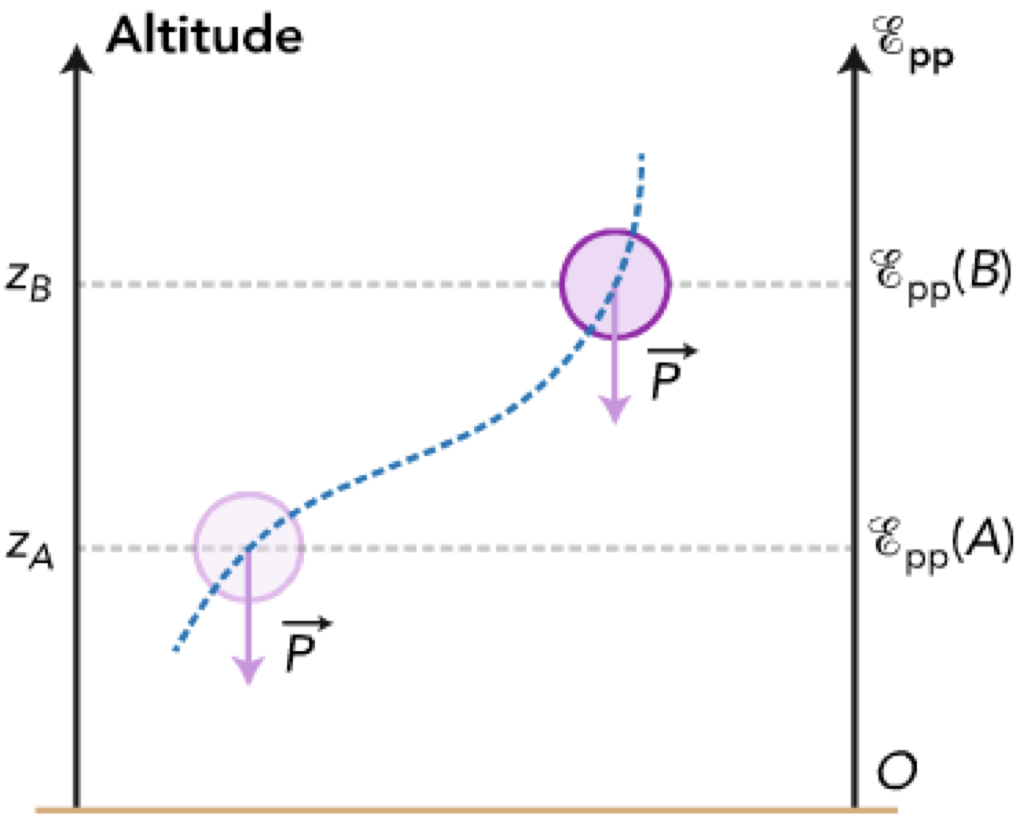
\includegraphics[scale=.4]{figures/travail_poids.png}	
 \end{center}
 
 

\blocrouge{Travail de la force électrique}{
La force électrique $\vec{F}=q\vec{E}$ est une force conservative. On retiendra que lorsqu'une charge $q$ se déplace de A vers B dans un champ électrique $\vec{E}$ son travail s'écrit: $$W(\vec{F})=\vec{F}\cdot\vec{AB} = \trou{q\times U_{AB}}$$
Unités: W en J ; q en C et $U_{AB}$ en V

}

\etiquette{Remarque} Dans les exercices, A et B désigneront généralement les plaques chargées entre lesquelles il existe un champ électrique $\vec{E}$. $U_{AB}$ est alors la tension entre ces plaques. Voir \textbf{livre p 245.}
\section{Théorème de l'énergie cinétique}
\subsection{Énoncé}
\blocrouge{Théorème de l'énergie cinétique}{La variation d'énergie cinétique d'un système qui se déplace d'un point A vers un point B est égale à la somme des \trou{travaux des forces} sur le trajet AB.$$Ec(B) - Ec(A) = \Sigma W_{A\rightarrow B}(\overrightarrow{F})$$
Cette année le système subit en général une force seule qui travaille il n'y aura pas de somme à effectuer. cf exercice
}
\subsection{Applications}

 \etiquette{Application 1}

On se place dans le cas d'une balle lâchée (sans vitesse initiale)  d'une hauteur  $h=5$ m. A l'instant $t_1=0$ s, la balle est lâchée et à l'instant $t_2$ elle touche le sol.
\begin{enumerate}
	\item Faire un schéma.
	\item Calculer le travail du poids pendant la chute.
	\item Ecrire le théorème de l'énergie cinétique et en déduire la valeur de la vitesse de la balle lorsque celle-ci atteint le sol.
\end{enumerate}


 \etiquette{Application 2}

 Une bille de masse m=50 g roule sur un support parfaitement glissant. Elle est lancée au point O à une vitesse de 4 m/s. Sur le trajet OA le support est parfaitement horizontal. Le trajet AB est incliné de $\SI{20}{\degree}$. Au point B, la bille rebrousse chemin puis commence à redescendre la pente. 

 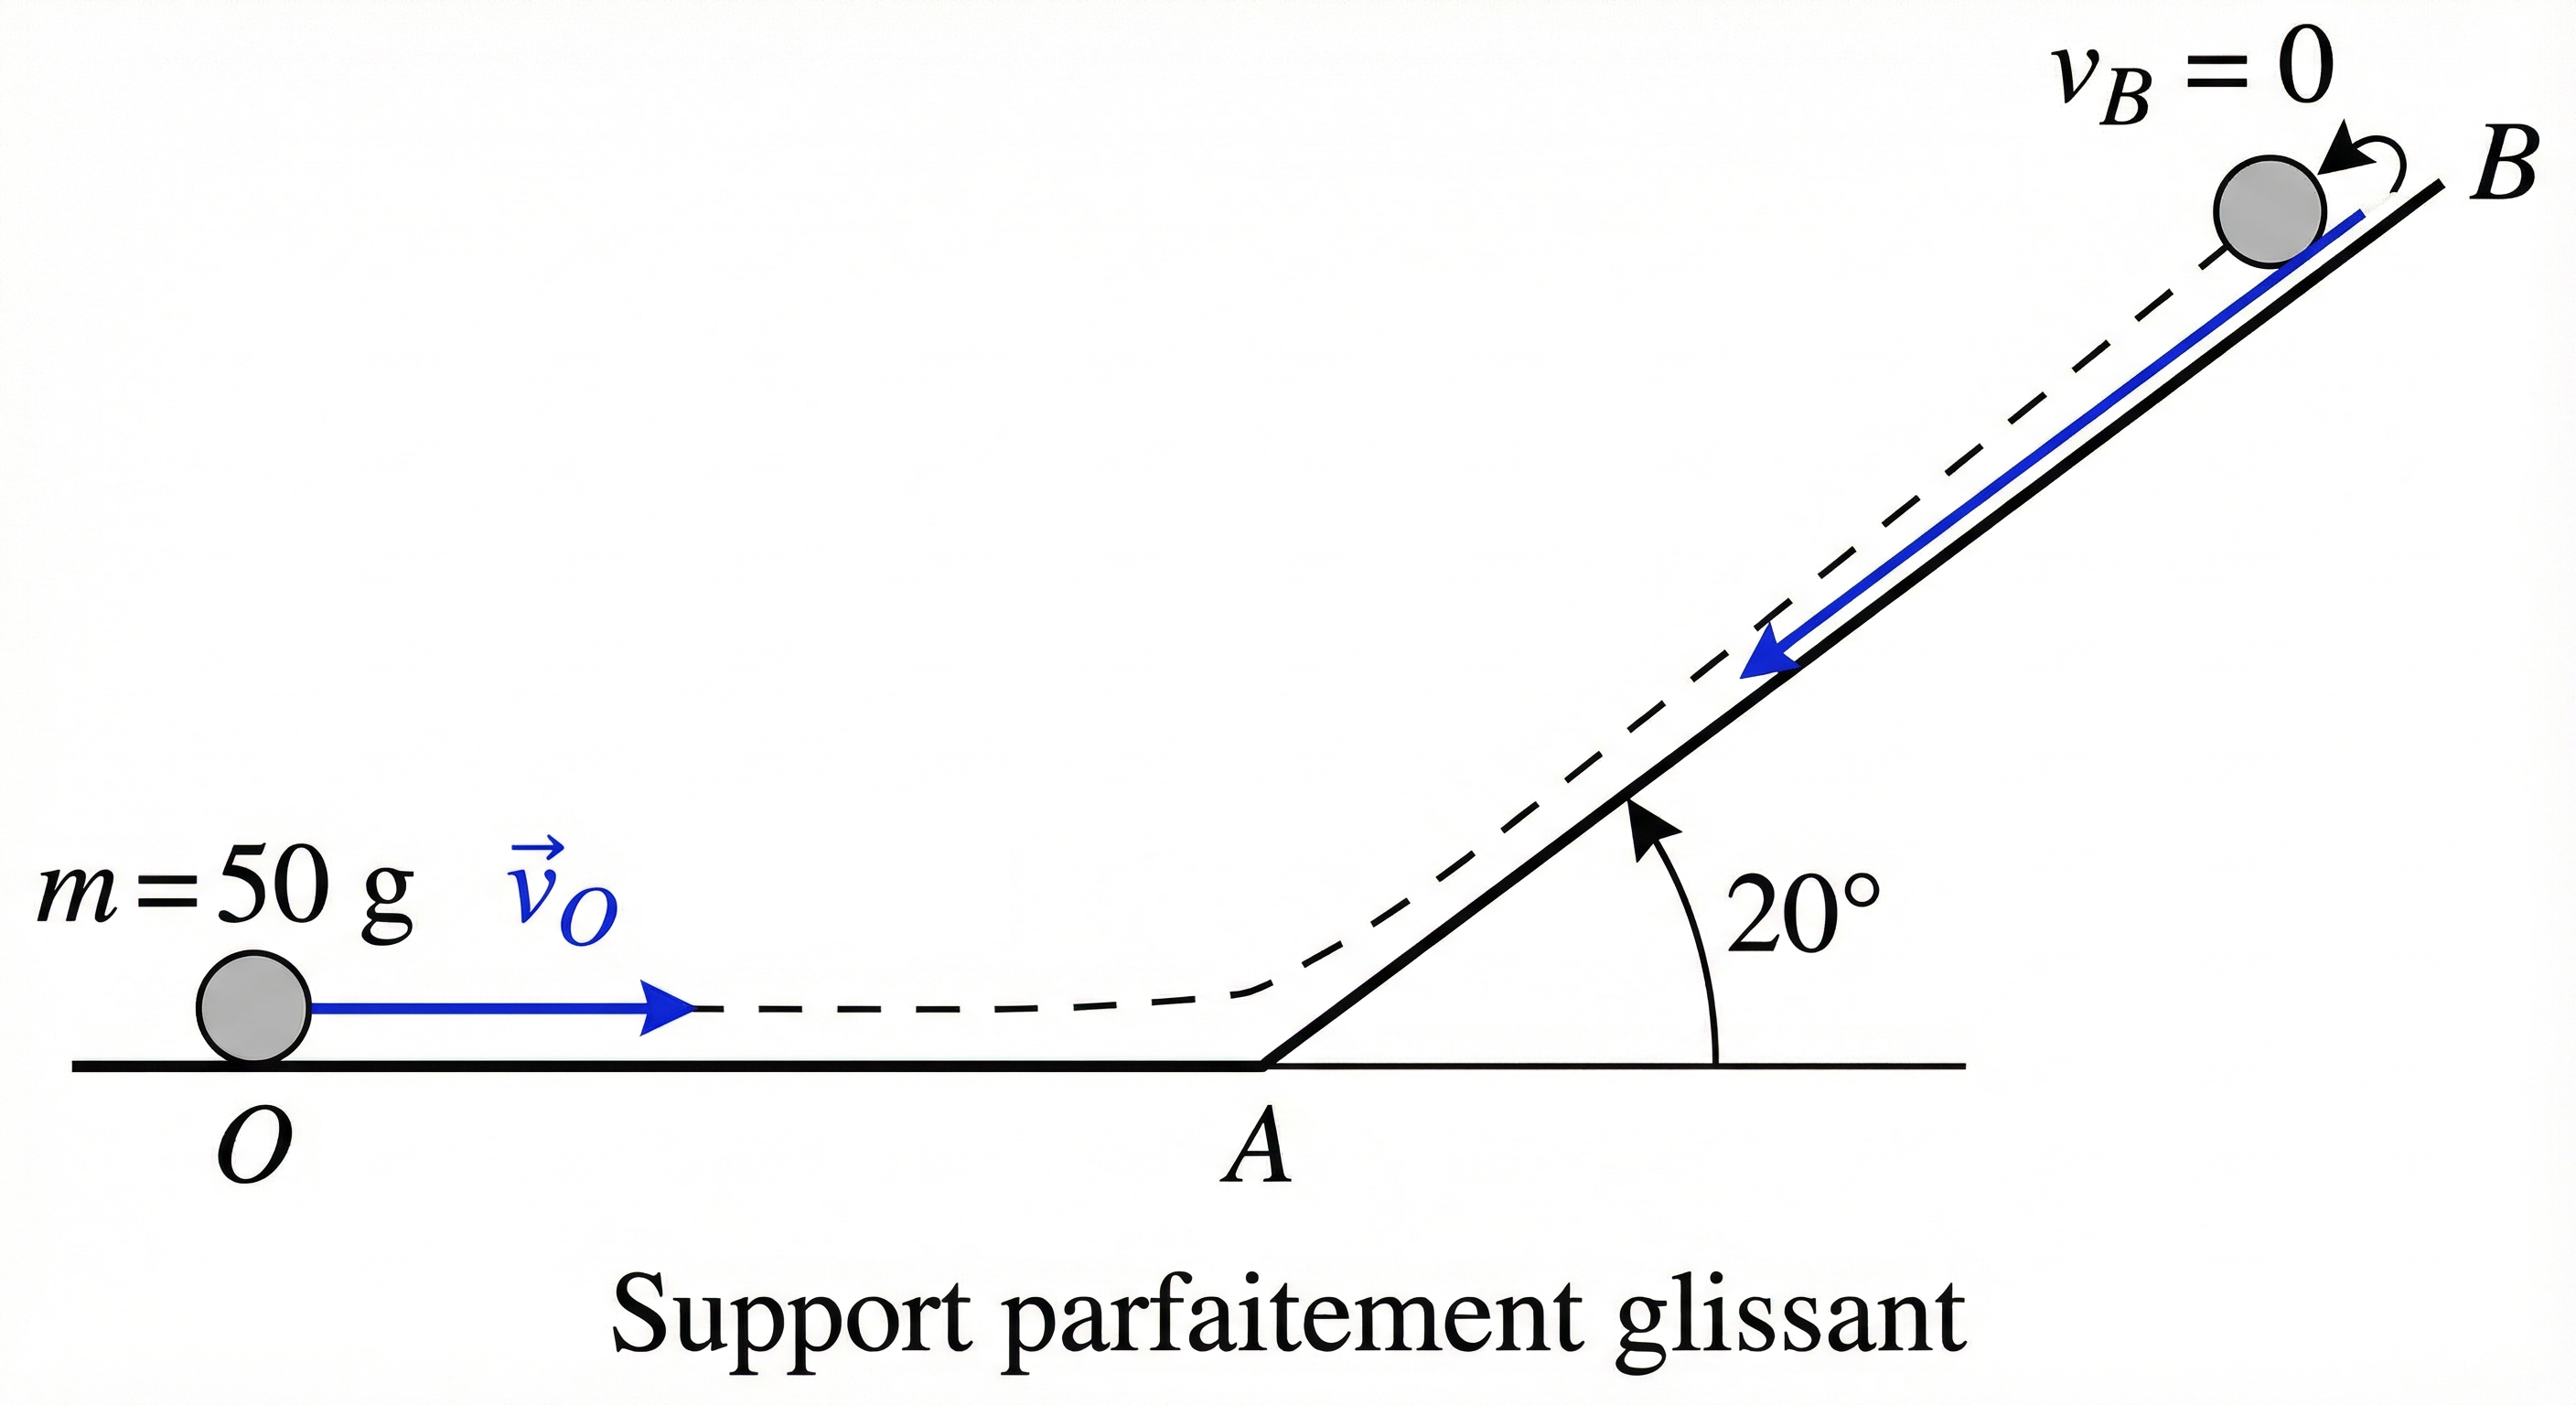
\includegraphics[width=10cm]{figures/fig_exo_energie.png}

 \begin{enumerate}

 	\item Faire le bilan des forces s'exerçant sur la bille.
 	\item Calculer les travaux des forces sur le trajet OA.
 	\item En utilisant le théorème de l'énergie cinétique, justifier que la vitesse de la bille en A est aussi de 4m/s.
 	\item Calculer la variation d'énergie cinétique entre A et B.
 	\item En déduire la valeur du travail du poids sur le trajet AB. 
 	\item Déterminer la distance AB.
 \end{enumerate}

 \etiquette{Application 3} Etude énergétique de l'accélération d'une particule chargée

On considère un proton initialement au repos en un point O. Ce proton est soumis au champ électrique $\vec{E}$ voir schéma. Les deux plaques sont soumises à une tension de 2,00 MV. Les plaques sont distantes de d=10,0 cm. 

\begin{center}
	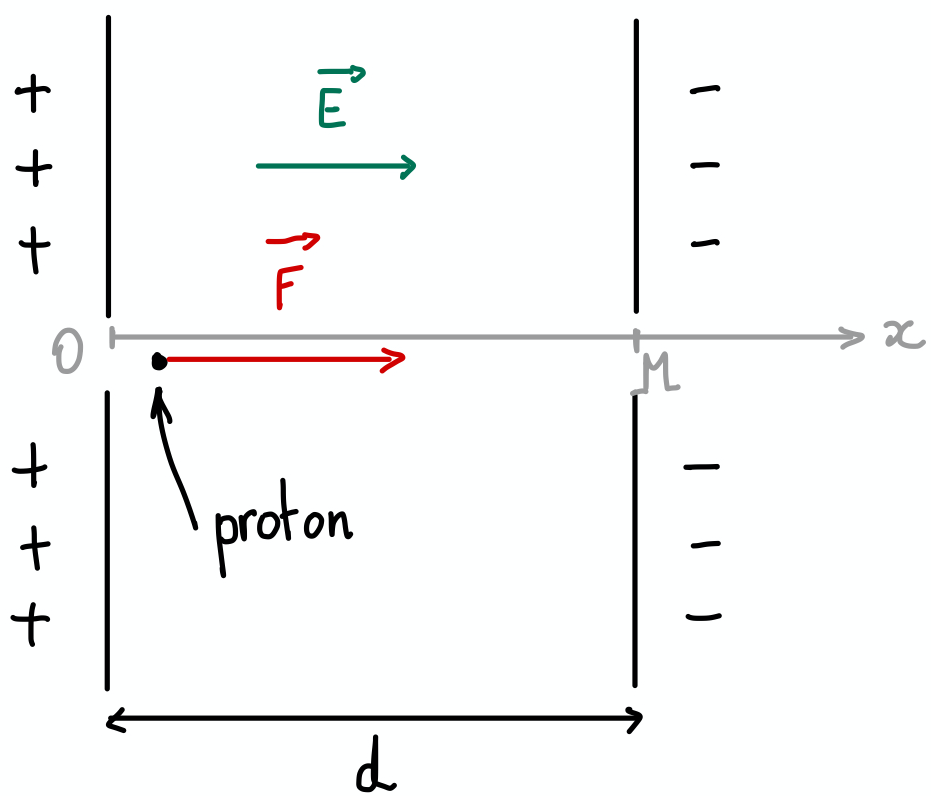
\includegraphics[height=4.5cm]{figures/dynamique/accelerateur_lineaire.png}

\end{center}


\etiquette{Objectif} Calculer la vitesse du proton au point M

\textbf{Plan de travail}
\begin{enumerate}
	\item Calculer le travail de la force électrique sur le déplacement de O vers M.
	\item Ecrire le théorème de l'énergie cinétique.
	\item Isoler la vitesse en M dans l'équation du théorème de l'énergie cinétique
\end{enumerate}

\textbf{Aides}
\begin{enumerate}
	\item 
	Utiliser la définition de la force électrique. Utiliser la définition du travail de la force sur le trajet $\vec{OM}$ $$W(\vec{F}) = \vec{F}  \cdot \overrightarrow{OM}$$ Le produit scalaire de deux vecteurs colinéaires et de même sens est égal au produit de leurs normes.
	\item $\Delta Ec = W(\vec{F})$
	\item $\Delta Ec = \frac{1}{2}mv_M^2$ et finalement $v_m= \sqrt{\frac{2qU}{m} }$
\end{enumerate}

\blocrouge{Travail personnel}{
\begin{itemize}
	\item Ex 24 et 25 p 254 et suivantes
	\item 2023 Réunion Sciences physiques pour les Sciences de l'ingénieur.e Jour 1 Lien: \url{https://www.labolycee.org/le-scanner-rayons-x}
	\item Vidéo présentant un exercice type bac:\\ \url{https://www.youtube.com/watch?v=LSX_AUg_MNQ}
	\item Imprimante à jet d'encre continu \\ \url{https://www.labolycee.org/imprimante-jet-dencre-continu}
	\end{itemize}
}

% \setcounter{chapter}{8}
\chapter{Forces des acides et bases}

\section{L'autoprotolyse de l'eau}
\subsection{L'eau, une espèce amphotère}
\blocrouge{Définition}{L'eau peut à la fois capter un ion $H^+$ ou en céder un. On dit que $H_2O$ est une espèce \trou{amphotère}}

Couples de l'eau : $H_3O^+/H_2O$ et $H_2O/HO^-$\\
L'eau peut donc être le seul réactif d'une réaction acide base appelée \textbf{l'autoprotolyse} de l'eau :

\begin{center}
$\trou{H_2O(l) + H_2O(l) \rightleftharpoons H_3O^+(aq) +HO^{-}(aq)}$	
\end{center}

\subsection{Le produit ionique de l'eau}

%Le pH de l'eau pure est égal à 7, ce qui signifie que $\rm [H_3O^+]=\trou{\SI{e-7}{\mole\per\liter}}$. Il y a donc présence d'ions $\rm[H_3O^+]$ dans l'eau. Ils proviennent de la réaction \trou{2\chemfig{H_2O} \chemrel{<>} \chemfig{H_3O^+} \chemsign+ \chemfig{HO^{-}}}\\
\blocrouge{Définition}{Pour toute solution aqueuse à l'équilibre chimique, on a $$\trou{\dfrac{\rm[H_3O^+]_{eq}\times[HO^{-}]_{eq}}{(c^o)^2}=10^{-14}=Ke}$$
Ke est appelé le produit ionique de l'eau. Par définition: $c^0=\SI{1}{\mol\per\liter}$. On y associe le pKe tel que $\rm pKe=-\log Ke=14$}


\section{Echelle des pH}

\subsection{Applications}
\etiquette{Situation 1}
On considère une solution dont le pH est égal à 3,5. 
\begin{enumerate}
	\item Cette solution est-elle acide, basique ou neutre ?\trou{cette solution est acide}
	\item Calculer $\rm[H_3O^+]_{eq}$ et $\rm[HO^-]_{eq}$. Comparer ces deux valeurs.
\end{enumerate}

\trou{$\rm[H_3O^+]_{eq}=10^{-3,5}=\SI{3,2e-4}{\mole\per\liter}$\\
$\rm[HO^-]_{eq}=\frac{Ke(c^0)^2}{[H_3O^+]_{eq}}=\frac{10^{-14}}{\num{3,2e-4}}=\SI{3,1e-11}{\mole\per\liter}$\\
On remarque que la concentration en ions $\rm H_3O^+$ est très supérieure à celle des ions $\rm HO^-$}

\etiquette{Situation 2} On considère  une solution de soude telle que $\rm[HO^-]_{eq}=\SI{1,0e-3}{\mole\per\liter}$.\\ Calculer $\rm[H_3O^+]_{eq}$ puis le pH\\
\trou{$\rm[H_3O^+]_{eq}=\frac{Ke(c^0)^2}{[HO^-]_{eq}}=\frac{10^{-14}}{\num{1,0e-3}}=\SI{1,0e-11}{\mole\per\liter}$\\
$\rm pH=-\log \num{1,0e-11}=11$}


\subsection{Échelle des pH}
\blocrouge{Définition}{
\includegraphics[scale=.80]{figures/acide_base/echelle_pH}

Solution neutre : \trou{$\rm[H_3O^+]_{eq}=[HO^-]_{eq}$ et $\rm pH=7$}\\
Solution acide : \trou{$\rm[H_3O^+]_{eq}>[HO^-]_{eq}$ et $\rm pH<7$}\\
Solution basique :\trou{ $\rm[H_3O^+]_{eq}<[HO^-]_{eq}$ et $\rm pH>7$}\\
}

\section{Réaction d'un acide ou d'une base avec l'eau}
\subsection{Cas des acides faibles - Réaction de l'acide éthanoïque avec l'eau}
\blocgris{Expérience}{
Nous introduisons $\SI{5,0e-4}{\mole}$ d'acide éthanoïque pur dans un $\SI{50}{\milli\liter}$ d'eau. Nous mesurons le pH de la solution, et nous trouvons pH=3,4.
}

Remplir le tableau d'évolution du système et en déduire si la transformation de l'acide éthanoïque avec l'eau est totale. : \\
\small
\begin{tabular}{|p{3cm}|p{1.5cm}|p{3cm}|p{1.2cm}|p{2cm}|p{2cm}|}
\hline 
  \multicolumn{2}{|c!{\protect\makebox[0cm]{:}}}{\textbf{Equation de la réaction}} &
 \multicolumn{1}{c!{\protect\makebox[0cm]{+}}}{%
      $\trou{\rm{CH_3COOH(aq)}}$} &
       \multicolumn{1}{c!{\protect\makebox[0cm]{ $\rightarrow$ }}}{%
      $\trou{\rm{H_2O(l)}}$} 
			&\multicolumn{1}{c!{\protect\makebox[0cm]{ + }}}
			{$\trou{\rm{CH_3COO^-(aq)}}$} 
			&\multicolumn{1}{c|}{
			$\trou{\rm{H_3O^+(aq)}}$} 
\tabularnewline


\hline 
Etat initial&
$x=0$&\trou{\num{5,0e-4}}
&\trou{excès}
&\trou{0}
&\trou{0}

\tabularnewline
\hline 
Etat intermédiaire&
$x$&\trou{\num{5,0e-4}-x}
&\trou{excès}
&\trou{x}
&\trou{x}

\tabularnewline
\hline 
Etat final= \textbf{Equilibre Chimique}&
$x=x_{f}$&$\rm \trou{\num{5,0e-4}-x_f}$
&\trou{excès}
&$\rm \trou{x_f}$
&$\rm \trou{x_f}$

\tabularnewline
\hline 
Etat final si la transformation était totale&
$x=x_{max}$&$\trou{\num{5,0e-4}-x_{max}}$
&\trou{excès}
&$\rm \trou{x_{max}}$
&$\rm \trou{x_{max}}$
\tabularnewline
\hline
\end{tabular}
\normalsize


$\trou{\rm x_f=[H_3O^+]_{eq} \times V=10^{-3,4}\times c^0 \times 0,050=\SI{2,0e-5}{\mol}}$\\

\etiquetterouge{Réfléchir!}
Ici $\rm x_f$ est différent de $\rm x_{max}$, ce qui signifie que la réaction n'est pas totale. La réaction atteint son état final (plus de consommation de réactif) alors que les deux réactifs sont encore présents. On dit que l'équilibre chimique est atteint. L'avancement à l'état final est donc inférieur à $x_{max}$ qui correspond à la consommation du réactif limitant.


\subsection{Cas des acides forts - Réaction de l'acide nitrique avec l'eau}

\blocgris{Expérience}{
Nous introduisons $\SI{5,0e-4}{\mole}$ d'acide nitrique pur dans un $\SI{50}{\milli\liter}$ d'eau. Nous mesurons le pH de la solution, et nous trouvons pH=2.
}


Remplir le tableau d'évolution du système et en déduire si la transformation de l'acide nitrique avec l'eau est totale. : 

\begin{tabular}{|p{3cm}|p{2cm}|p{3cm}|p{2cm}|p{1.5cm}|p{1.5cm}|}
\hline 
  \multicolumn{2}{|c!{\protect\makebox[0cm]{:}}}{\textbf{Equation de la réaction}} &
 \multicolumn{1}{c!{\protect\makebox[0cm]{+}}}{%
      $\trou{\rm HNO_3}$} &
       \multicolumn{1}{c!{\protect\makebox[0cm]{ $\rightarrow$ }}}{%
      $\trou{\rm{H_2O(l)}}$} 
			&\multicolumn{1}{c!{\protect\makebox[0cm]{ + }}}
			{$\trou{\rm NO_3^-}$} 
			&\multicolumn{1}{c|}{
			$\trou{\rm H_3O^+}$} 
\tabularnewline


\hline 
Etat initial&
$x=0$&\trou{\num{5,0e-4}}
&\trou{excès}
&\trou{0}
&\trou{0}

\tabularnewline
\hline 
Etat intermédiaire&
$x$&\trou{\num{5,0e-4}-x}
&\trou{excès}
&\trou{x}
&\trou{x}

\tabularnewline
\hline 
Etat final&
$x=x_{f}$&$\rm \trou{\num{5,0e-4}-x_f}$
&\trou{excès}
&$\rm \trou{x_f}$
&$\rm \trou{x_f}$

\tabularnewline
\hline 
Etat final si la transformation était totale&
$x=x_{max}$&$\trou{\num{5,0e-4}-x_{max}}$
&\trou{excès}
&$\rm \trou{x_{max}}$
&$\rm \trou{x_{max}}$
\tabularnewline
\hline
\end{tabular}


\trou{$\rm x_f=[H_3O^+]_{eq} \times V=10^{-2}\times c^0 \times 0,050=\SI{5,0e-4}{\mole}$\\
On remarque que $\rm x_f= x_{max}$, ce qui signifie que la réaction est totale..}
\subsection{Conclusion}

\etiquetterouge{Acide fort ou acide faible ?}


 Lorsque l'on introduit un acide dans l'eau, deux cas sont possibles : 
\begin{enumerate}
\item
Sa réaction avec l'eau est totale.\\On parle alors d'acide fort.\\On écrit : $$\trou{HA(aq) + H_2O(l) \longrightarrow H_3O^+(aq) + A^{-}(aq)}$$
C'est le cas de l'acide nitrique : $$ HNO_3(aq)+H_2O(l) \longrightarrow H_3O^+(aq) + NO_3^{-}(aq)$$


\item 
Sa réaction avec l'eau n'est pas totale.\\
On parle alors d'acide faible.\\On écrit :
$$HA(aq) + H_2O(l) \rightleftharpoons \trou{H_3O^+(aq) }+ \trou{A^{-}(aq) }$$
C'est le cas de l'acide éthanoïque :
$$ CH_3COOH(aq) + H_2O(l) \rightleftharpoons \trou{H_3O^+(aq) + CH_3COO^{-}(aq)}$$

\end{enumerate}

\subsection{Réaction d'une base avec l'eau}

On raisonne par analogie à ce que l'on a appris sur la réaction entre un acide et l'eau.\\
Lorsque l'on introduit une base dans l'eau, deux cas sont possibles : 
\begin{itemize}
\item
Sa réaction avec l'eau est totale.\\On parle alors de \trou{ base forte}.\\On écrit :  $$ A^-(aq) + H_2O(l) \longrightarrow AH(aq) + HO^{-}(aq)$$
\item 
Sa réaction avec l'eau n'est pas totale.\\
On parle alors de \trou{base faible}.\\On écrit :  $$ A^-(aq) + H_2O(l)\rightleftharpoons  AH(aq) + HO^{-}(aq)$$
\end{itemize}

\section{Calculer le pH des solutions d'acide fort et de base forte}

\etiquette{Situation} Lors de la préparation d'une solution d'acide ou de base, il y a eu réaction chimique entre le soluté (l'acide ou la base) et le solvant ($H_2O$).

L'état initial est le moment où l'on apporte une certaine quantité de matière de soluté. Celle-ci est notée $n_0$ dans la suite. 
Lorsque l'on prépare un volume V de solution à partir de $n_0$, on obtient une solution de concentration en soluté apporté C tel que $$C=\frac{n_0}{V}$$


\subsection{Cas d'un Acide FORT}

On considère une solution d'acide HA de concentration $\rm C$ et de volume V. \\
\begin{tabular}{|l|p{2cm}|p{2cm}|p{2cm}|p{2cm}|p{2cm}|}
\hline 
  \multicolumn{2}{|c!{\protect\makebox[0cm]{:}}}{\textbf{Equation de la réaction}} &
 \multicolumn{1}{c!{\protect\makebox[0cm]{+}}}{%
      $\trou{\rm HA}$} &
       \multicolumn{1}{c!{\protect\makebox[0cm]{ $\rightarrow$ }}}{%
      $\trou{\rm{H_2O(l)}}$} 
			&\multicolumn{1}{c!{\protect\makebox[0cm]{ + }}}
			{$\trou{\rm A^-}$} 
			&\multicolumn{1}{c|}{
			$\trou{\rm H_3O^+}$} 
\tabularnewline


\hline 
Etat initial&
$x=0$&\trou{$\rm CV= n_0$}
&\trou{excès}
&\trou{0}
&\trou{0}

\tabularnewline
\hline 
Etat intermédiaire&
$x$&\trou{$\rm CV-x$}
&\trou{excès}
&\trou{x}
&\trou{x}


\tabularnewline
\hline 
Etat final&
$x=x_{max}$&$\trou{CV-x_{max}}$
&\trou{excès}
&$\rm \trou{x_{max}}$
&$\rm \trou{x_{max}}$
\tabularnewline
\hline
\end{tabular}\\
La réaction est totale donc on obtient $\rm x_{max}=\trou{CV = n_0 = n(H_3O^+)_{eq}}$.\\
On a alors $\trou{\rm [H_3O^+]_{eq}=\frac{CV}{V}=C}$ et $\rm pH=-\log \dfrac{C}{c^0}$

\blocrouge{Conclusion}{
Le pH d'une solution d'acide fort est tel que $$\trou{\rm pH=-\log \dfrac{C}{c^0}}$$ avec $\rm C$ la concentration en acide de la solution.}


\subsection{Cas d'une base FORTE}
On considère une solution de base forte notée $\rm A^-$ de concentration $\rm C$ et de volume V. \\
\begin{tabular}{|p{3cm}|p{2cm}|p{2cm}|p{2cm}|p{2cm}|p{2cm}|}
\hline 
  \multicolumn{2}{|c!{\protect\makebox[0cm]{:}}}{\textbf{Equation de la réaction}} &
 \multicolumn{1}{c!{\protect\makebox[0cm]{+}}}{%
      $\trou{\rm A^-}$} &
       \multicolumn{1}{c!{\protect\makebox[0cm]{ $\rightarrow$ }}}{%
      $\trou{\rm{H_2O(l)}}$} 
			&\multicolumn{1}{c!{\protect\makebox[0cm]{ + }}}
			{$\trou{\rm AH}$} 
			&\multicolumn{1}{c|}{
			$\trou{\rm HO^-}$} 
\tabularnewline


\hline 
Etat initial&
$x=0$&\trou{$\rm CV = n_0$}
&\trou{excès}
&\trou{0}
&\trou{0}

\tabularnewline
\hline 
Etat intermédiaire&
$x$&$\trou{\rm CV-x}$
&\trou{excès}
&\trou{x}
&\trou{x}


\tabularnewline
\hline 
Etat final &
$x=x_{max}$&$\trou{CV-x_{max}}$
&\trou{excès}
&$\rm \trou{x_{max}}$
&$\rm \trou{x_{max}}$
\tabularnewline
\hline
\end{tabular}

La réaction est totale donc $x_f=x_{max}=n_0=C\times V$ \\
A l'état final, on a $\trou{\rm [HO^-]=C}$ et $[H_3O^+]=\frac{Ke}{C}\times (c^0)^2$ et $\dfrac{[H_3O^+]}{c^0}=\frac{Ke}{C}\times (c^0)$ .\\On a donc $\trou{-\log \dfrac{[H_3O^+]}{c^0}} =-\log Ke + \log \dfrac{C}{c^0}$ et $\rm pH=pKe+\log \dfrac{C}{c^0}$

\blocrouge{Conclusion}{
Le pH d'une solution de base forte est tel que $\rm pH=pKe+\log \dfrac{C}{c^0}$ avec $\rm C$ la concentration en base de la solution.
}



\section{Force d'un acide}
\subsection{Taux d'avancement}

\blocrouge{Définition}{ Pour indiquer l'aspect total ou limité d'une réaction on calcule le taux d'avancement $$\tau=\dfrac{x_f}{x_{max}}$$}

Si $\tau<1$ alors \trou{la réaction n'est pas totale}. Si $\tau=1$ alors \trou{la réaction est totale.}

Plus le taux d'avancement de la réaction d'un acide avec l'eau est proche de 1 plus cet acide se comporte comme un acide fort. Même raisonnement pour une base.
\subsection{Constante Ka}

\blocrouge{Définitions}{
Soit un couple $\rm HA(aq)/A^-(aq)$ dont l'acide réagit avec l'eau selon la réaction d'équation\\
$$\trou{HA(aq)} + \trou{H_2O(l)} \rightleftarrows H_3O^+(aq) + A^{-}(aq)$$

La constante d'acidité notée Ka du couple est définie par :\\
$$\rm Ka=\trou{\frac{[A^-]_{eq}\times[H_3O^+]_{eq}}{[HA]_{eq}\times c^0}}$$\\
Avec $\rm[A^-]_{eq}$,$\rm[H_3O^+]_{eq}$et$\rm[HA]_{eq}$ les valeurs des  concentrations lorsque le système a atteint son état d'équilibre.\\
On définit également le pKa tel que $\rm pKa=\trou{-\log Ka}$ et par conséquent, $\rm Ka=\trou{10^{-pKa}}$
}

Quelques exemples : \\
\begin{tabular}{|c|c|c|}
\hline
Couple Acide/Base &Ka&pKa\\
\hline
$\rm CH_3COOH/CH_3COO^-$&$\rm \trou{10^{-4,8}}$&4,8\\
\hline
$\rm HCOOH/HCOO^-$&$\rm10^{-3,8}$&\trou{3,8}\\
\hline
$\rm NH_4^+/NH_3$&$\rm \trou{10^{-9,2}}$&9,2\\
\hline
\end{tabular}
\blocgris{Technique importante}{ Comment prévoir la composition chimique d'une solution d'acide connaissant sa concentration et son Ka ?\\
On considère une solution d'acide méthanoïque de concentration égale à $c=\SI{1,0e-2}{\mole\per\liter}$. A partir de la valeur du Ka, retrouver la valeur des concentrations de toutes les espèces chimiques présentes à l'équilibre.
}



\subsection{Classement des acides}
\begin{minipage}{0,65\linewidth}
Un acide est d'autant plus fort que le taux d'avancement de sa réaction avec l'eau est \trou{grand}.\\
$\rm Ka=\trou{\frac{[A^-]_{eq}\times[H_3O^+]_{eq}}{[HA]_{eq}\times c^0}}$\\
Donc, plus un acide est fort, plus :
\begin{itemize}
\item$ [A^-]_{eq}$ sera \trou{élevée}
\item$ [H_3O^+]_{eq}$ sera \trou{élevée}
\item $ [HA]_{eq}$ sera \trou{faible}
\end{itemize}
On en déduit, que plus un acide est fort (et plus sa base conjuguée est faible) plus sa constante d'acidité Ka est \trou{grande}, et par conséquent, plus son pKa est \trou{faible}.
\end{minipage}
\begin{minipage}{0,4\linewidth}
\begin{center}
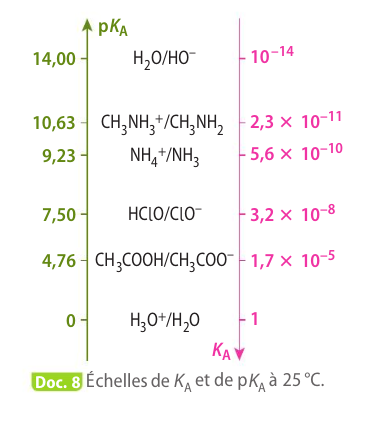
\includegraphics[scale=0.4]{figures/acide_base/fig_pka}
\end{center}
\end{minipage}


\blocrouge{Conclusion}{
Plus la constante d'acidité Ka d'un couple acide-base $AH/A^-$ est grande, plus son pKa est \trou{petit}, plus la force de l'acide AH est \trou{élevée} et plus la force de la base $A^-$ est \trou{faible}.}

\subsection{Diagramme de prédominance}
\etiquetterouge{Définition}\\
Une espèce est prédominante devant une autre espèce si \trou{sa concentration en solution est plus grande que celle de l'autre espèce.}
\\
Afin d'identifier la prédominance d'une espèce d'un couple acide base connaissant son pH et son pKa, nous allons établir la relation entre le pH et le pKa d'un couple.\\ En vous aidant des rappels mathématiques sur la fonction log, montrer que $$\rm pH=pKa + \log \frac{[A^-]_{eq}}{[HA]_{eq}}$$ 

\trou{
$\rm Ka=\frac{[A^-]_{eq}\times[H_3O^+]_{eq}}{[HA]_{eq}\times c^0}$ donc\\
$\rm \dfrac{[H_3O^+]_{eq}}{c^0}=Ka\times\frac{[HA]_{eq}}{[A^-]_{eq}}$\\
$\rm \log \dfrac{[H_3O^+]_{eq}}{c^0}=\log Ka + \log \frac{[HA]_{eq}}{[A^-]_{eq}}$\\
$\rm - \log  \dfrac{[H_3O^+]_{eq}}{c^0}=-\log Ka - \log \frac{[HA]_{eq}}{[A^-]_{eq}}$\\
$\rm pH=pKa + \log \frac{[A^-]_{eq}}{[HA]_{eq}}$\\}

\begin{itemize}
\item
Si pH=pKa, \trou{$\rm \log\frac{[A^-]_{eq}}{[HA]_{eq}}=0$, et $\rm [A^-]_{eq}=[HA]_{eq}$.Les concentrations sont égales, aucune espèce ne prédomine.}
\item Si pH>pKa,\trou{ $\rm \log\frac{[A^-]_{eq}}{[HA]_{eq}}>0$, et $\rm \frac{[A^-]_{eq}}{[HA]_{eq}}>1$ donc $\rm [A^-]_{eq}>[HA]_{eq}$ donc la base prédomine.}
\item Si pH<pKa, \trou{$\rm \log\frac{[A^-]_{eq}}{[HA]_{eq}}<0$, et $\rm \frac{[A^-]_{eq}}{[HA]_{eq}}<1$ donc $\rm [A^-]_{eq}<[HA]_{eq}$ donc l'acide prédomine.}
\end{itemize}

\vspace{1cm}


Diagramme de prédominance :  \\
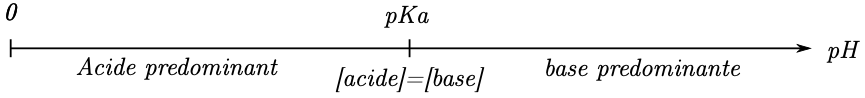
\includegraphics[scale=.5]{figures/acide_base/diag_predominance}

\etiquette{Application}: Réaliser les diagrammes de prédominance des couples suivants :\\
\textbf{Dans la famille : acide carboxylique/ion carboxylate} : $\rm{RCOOH/RCOO^-}$\\
Exemple de l'acide méthanoïque de pKa égal à 3,8.\\
\textbf{Dans la famille : amine/ion ammonium} : $\rm{RNH_3^+/RNH_2}$\\
Exemple de la méthylamine de pKa égal à 10,6.\\
Exemple de la diméthylamine de pKa égal à 10,8

\subsection*{Le cas des acides $\alpha$aminés}
La valine est un acide $\alpha$aminé. L'une de ses formes acido-basiques est la suivante :\\
\chemfig{CH(-[2]CH_3)(-[4]H_3C)-CH(-[2]CO_2H)-NH_3^+}\\

On lui attribue deux pKa : 2,3 et 9,7.
\begin{enumerate}
\item Entourer les groupes caractéristiques de la valine qui possèdent des propriétés acido-basiques.
\item Quel groupe caractéristique est responsable du pKa le plus petit ? le plus grand ?
\item Ecrire les 4 formes de la valine théoriquement possibles.
\item Tracer le diagramme de prédominance de la valine en fonction du pKa égal à 2,3.
\item Sous ce diagramme, tracer le diagramme de prédominance en fonction du pKa égal à 9,7.
\item En étudiant les diagrammes tracés précédemment, montrer que l'une des formes trouvées à la question 3 n'existe pas.
\item La valine est abondante dans le blanc d'\oe uf, dont le pH est voisin de 7,5. Sous quelle forme acido-basique trouve-t-on majoritairement la valine dans le blanc d'\oe uf ?
\end{enumerate}


\subsection{Diagramme de distribution}
\begin{minipage}{0,6\linewidth}
Le diagramme de distribution représente les pourcentages d'un acide et de sa base conjuguée en fonction de la valeur du pH. Il permet de connaître la composition d'un système à un instant donné.\\
Lorsque l'acide et sa base conjuguée sont en proportions égales, le pH est égal au \trou{pKa} du couple.
\end{minipage}
\begin{minipage}{0,4\linewidth}
\begin{center}
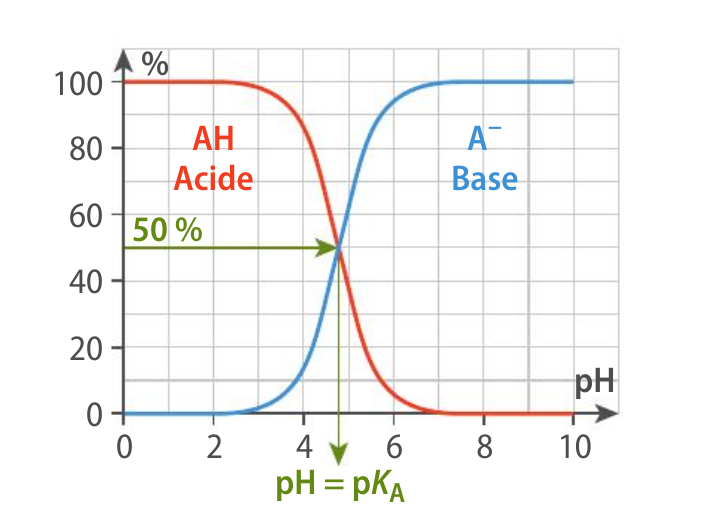
\includegraphics[scale=0.3]{figures/acide_base/fig_diag_distrib}
\end{center}

\end{minipage}

\subsection{Cas des indicateurs colorés}

Un indicateur coloré est une solution contenant un couple dont l'acide et la base conjuguée ont des teintes différentes. Sa zone de virage correspond à l'intervalle de pH dans lequel il passe d'une forme à l'autre. \\
\begin{center}
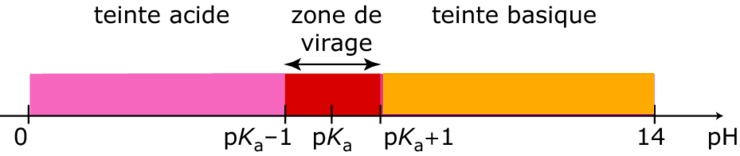
\includegraphics[scale=1.2]{figures/acide_base/fig_indic_color.jpg}
\end{center}

Un indicateur coloré peut être utilisé pour déterminer l'équivalence d'un titrage acide-base si le pH à l'équivalence se situe dans la zone de virage.

\section{Les solutions à connaître}
\subsection{Solution tampon}
\blocrouge{Définition}{
\trou{Une solution tampon est une solution dont le pH varie peu à l'ajout d'une petite quantité de base, d'acide ou d'eau}
}

Les solutions tampons permettent de contrôler la valeur du pH notamment lors de l'étalonnage d'un pH-mètre.

\subsection{Les petits basiques à connaître..}

\begin{tabular}{|c|p{5cm}|}
\hline
Nom de la solution&Formule chimique\\
\hline
acide chlorhydrique&\\
\hline
acide nitrique&\\
\hline
hydroxyde de sodium ou soude&\\
\hline
acide éthanoïque&\\
\hline
ammoniac&\\
\hline
\end{tabular}

\section*{Exercices à faire}

1 p 162
11, 14, 15 p 165
19 , 25 p 166-168

Bilan: 31 p 170

Type Bac: \url{https://www.labolycee.org/etude-de-lacide-benzoique-et-du-benzoate-de-sodium} Partie A

% \setcounter{chapter}{9}
\chapter{Les Ondes}

\section{Rappels}
\subsection{Onde mécanique progressive ?}

En secouant l'extrémité d'une corde, on observe que la perturbation créée se déplace le long de la corde. Ce phénomène s'appelle la \emph{propagation}. 

Bien que l'onde se propage, la corde ne se déplace pas dans son ensemble. On dit qu'il n'y a pas de transport de matière. 

\blocrouge{Définition}{On appelle onde mécanique, la \trou{propagation d'une perturbation dans un milieu matériel}, sans {transport de matière} et avec transport d'énergie.}



\blocrouge{Définition}{
	\begin{itemize}
%		\item L'\textbf{amplitude} de la déformation caractérise l'écart entre l'équilibre du milieu et la déformation.
		\item La vitesse de propagation $v$ est la vitesse à laquelle se déplace la perturbation. Elle s'exprime en m/s. On l'appelle aussi \textbf{célérité} et on la note parfois $c$.
	\end{itemize}
}

\subsection{Retard d'une onde}

Prenons en photo une corde secouée à deux instants $t$ et $t'$ avec $t<t'$. A l'instant $t$ la perturbation est au point M de la corde. Ensuite la perturbation va toucher d'autres points de la corde en se propageant et M retourne à sa position de repos. A l'instant $t'$, la perturbation a atteint le point $M'$ de la corde.

\begin{center}
	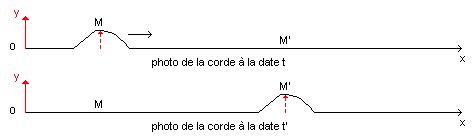
\includegraphics{figures/ondes/retard}
\end{center}

\blocrouge{Vocabulaire}{On appelle retard la durée mise par la perturbation pour aller de $M$ à $M'$ . On dit que le point $M'$ est en \trou{\textbf{retard}} par rapport à $M$. }

\paragraph*{Calcul d'un retard}

On note $d$ la distance entre $M$ et $M'$. On note $\Delta t$ la durée qui s'écoule entre l'instant $t$ et l'instant $t'$. Dans ce cas, la vitesse de l'onde est $$c=\frac{d}{\Delta t}$$ Le retard vaut donc $$\boxed{\trou{\Delta t = \frac{d}{c}}}$$



\section{Ondes progressives périodiques}

Etudier la simulation \url{https://phet.colorado.edu/fr/simulation/wave-on-a-string}
 
\blocrouge{Définitions}{La période temporelle notée $T$ est la plus petite durée, au bout de laquelle, un phénomène se \trou{reproduit identiquement à lui même}. Elle s'exprime en seconde: s.\\
On utilise aussi la fréquence $f$ qui est reliée à la période $T$ selon: $$f=\frac{1}{T}$$ f s'exprime en Hz ou $s^{-1}$.}

 
\paragraph*{Conséquence:}Au bout d'une durée T, tous les points se retrouvent à nouveau dans le même état vibratoire.\\

\subsection{Périodicité spatiale ou longueur d'onde: $\lambda$}
En observant l'onde à un instant $t$ donné, on observe une périodicité tout au long de l'onde. C'est la longueur d'onde: $\lambda$. 

\blocrouge{Définition}{La longueur d'onde $\lambda$ est la plus petite distance entre deux points successifs qui \trou{vibrent en phase} (même état vibratoire à tout instant)}

 C'est aussi la \trou{taille du motif} qui se répète si on observe une photo de l'onde.

\subsection{Relation entre $\lambda$ et $T$}
\begin{center}
	\includegraphics{figures/ondes/fig_relation_propag}
\end{center}

Entre la première et la troisième représentation de l'onde il s'est écoulé une durée égale à T. Pendant ce temps, la perturbation a parcouru une distance égale à $\lambda$ à la vitesse $c$.

\blocrouge{Relation entre période, longueur d'onde et célérité}{$$c=\trou{\frac{\lambda}{T}}$$  
Unités: $\lambda$ en m ; T en s et c en m/s ou \SI{}{\meter\per\second}
}


\section{Le niveau d'intensité sonore}
\subsection{Puissance, intensité, niveau}
Soit une source sonore de puissance P, plus on s'éloigne de la source sonore, plus le son entendu est faible car la puissance sonore se répartit sur une sphère de surface S de plus en plus grande. \\
Donc, on peut poser I l'intensité sonore telle que \begin{center}
\trou{$I=\frac{P}{S}$ }
\end{center}
avec\trou{  P en watts, S en $\si{\meter\squared}$ et I en $\si{\watt\per\meter\squared}$.}
	
	
	\blocrouge{Définition}{
	Le niveau sonore est une grandeur liée à la sensation auditive. Il s'exprime en dB et est défini par la relation : 

	$$\trou{L=10\log\left(\frac{I}{I_0}\right)}$$
$I_0=\SI{e-12}{\watt\per\meter\squared}$ est le seuil d'audibilité.\\
	Par conséquent, on a également 


	$$	\trou{I=I_0\times 10^{L/10}}$$
}

	
	
	\begin{center}
		\includegraphics[scale=0.4]{figures/ondes/fig2.pdf}
	\end{center}


\blocgris{Application}{
Une trompette émet un son dont le niveau sonore vaut : 60 dB. Calculer l'intensité sonore du son de la trompette.\trou{$\SI{e-8}{\watt\per\meter\squared}$}\\ On
fait jouer trois trompettes. Que vaut l'intensité sonore, que vaut le niveau sonore ?\trou{64,8 dB}Conclure sur la linéarité du niveau sonore.\\
Que vaut le rapport : $\frac{I'}{I}$ entre deux sons pour passer de 60 dB à 80 dB ? A combien de trompettes cela correspond-il ? \trou{100}
}

\subsection{Atténuation}
Si l'on s'éloigne de la source sonore ou que l'on place un objet entre la source et notre oreille, le son est atténué. On parle d'atténuation d'un son.
L'atténuation est égale à la différence entre le niveau sonore avant atténuation et le niveau sonore après atténuation.\\
On a donc : \begin{center}
\trou{$A=L_i-L_f$}
\end{center} 
et aussi :\begin{center}
\trou{$A=10 \log\left( \dfrac{I_i}{I_f}\right)$}
\end{center}  avec $I_i$ et $I_f$ les intensités sonores aux instants initiaux et finaux en $\SI{}{\watt\per\meter\squared}$\\
\begin{minipage}{0,7\linewidth}


L'atténuation peut être géométrique, elle est alors due à l'éloignement de la source puisque la surface S sur laquelle se répartit l'onde est de plus en plus grande.\\

L'atténuation peut aussi se faire par absorption, elle est alors due à l'absorption d'une partie de la puissance sonore par un milieu matériel traversé par l'onde.
\end{minipage}
\begin{minipage}{0,3\linewidth}
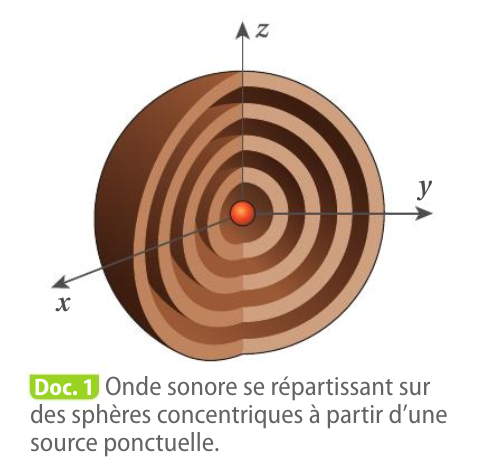
\includegraphics[scale=0.3]{figures/ondes/attenuation.png}
\end{minipage}

\etiquette{Exercices}\\
2,3,7,20 et 21 p 357 et suivantes

\section{Effet Doppler}
\subsection{Présentation}
\blocrouge{Définition}{L'effet Doppler est l'existence d'un décalage entre la fréquence d'une onde émise $f_E$ et la fréquence de l'onde reçue $f_R$ lorsque la distance entre l'émetteur et le récepteur varie.\\ L'écart de fréquence est appelé : décalage Doppler et vaut $\Delta f=f_R-f_E$}

\subsection{Deux situations}
A gauche de la figure, la source est immobile par rapport à l'observateur. Les fronts d'onde sont éloignés de $\lambda$. \\ A droite, l'émetteur se rapproche de l'observateur. La distance entre deux fronts d'onde perçus par l'observateur est plus petite que $\lambda$ donc la fréquence plus grande car $f=c/\lambda$

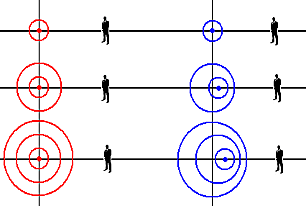
\includegraphics{gfx/Ondes_2012/effet-doppler}

\begin{enumerate}
	\item L'émetteur se rapproche du récepteur alors $f_R>f_E$. \\ Exemple: Lorsque la sirène de l'ambulance se rapproche on perçoit un son plus aigu que lorsque l'ambulance est immobile.
	\item Si l'émetteur s'éloigne du récepteur alors $f_R<f_E$. \\ Exemple: Lorsque la sirène de l'ambulance s'éloigne on perçoit un son plus grave que lorsque l'ambulance est immobile.
\end{enumerate}

\etiquette{Lire p 352}

\etiquetterouge{Démonstration} Livre p 253 et Exercice 24 p 362

\subsection{Application}
L'effet Doppler s'observe aussi bien pour les ondes mécaniques que pour les ondes électromagnétiques. 
\etiquette{Culture}

Les raies du spectre d'une étoile qui s'éloigne de la Terre sont perçues décalées en comparaison avec celles mesurées depuis une source immobile. Ce décalage peut être utilisé pour la mesure d'une vitesse d'éloignement. 
Le décalage vers le rouge des radiations émises par les Galaxies vers la Terre valide l'hypothèse d'un univers en expansion (Les galaxies s'éloignent toutes de la Terre).

L'effet Doppler est aussi utilisé avec des ultrasons pour mesurer la vitesse des globules rouge dans le sang lors d'échographie. 

\etiquette{Exercices}
\begin{itemize}
	\item Ex 10 p 359
	\item Ex 22 p 361
	\item Ex 26 p 263
\end{itemize}
\section{La diffraction} 
\subsection{Observation du phénomène}
\blocgris{Expérience}{
Observation du phénomène de diffraction avec la cuve à onde\\
On place sur le trajet des ondes un obstacle présentant une petite ouverture.\\
On observe \trou{un étalement des directions de propagation de l'onde. L'onde est diffractée}\\
Que se passe-t-il si l'on agrandit l'ouverture ?\\
\trou{le phénomène de diffraction ne s'observe plus}
}

\begin{center}
 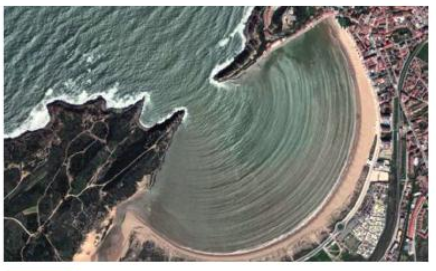
\includegraphics[scale=0.5]{figures/ondes/fig_diff_baie}
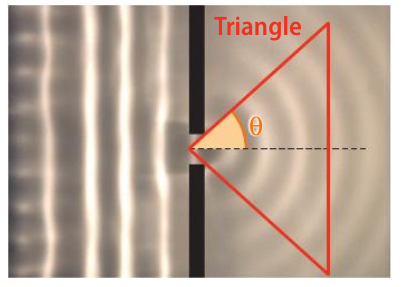
\includegraphics[scale=0.5]{figures/ondes/fig_diff_theta}
\end{center}

On nomme l'angle $\theta$ \textbf{angle caractéristique de diffraction}. Il met en évidence l'importance du phénomène de diffraction.
\blocrouge{Conclusion}{
\trou{
Lorsqu'une onde franchit un obstacle \textbf{de taille comparable ou inférieure à sa longueur d'onde}, on observe un éparpillement de l'onde. On parle de diffraction.
Plus l'ouverture est petite, plus l'angle $\theta$ est grand et plus le phénomène de diffraction est important. }

}

\subsection{Cas des ondes lumineuses}
\blocgris{Expérience}{
Observation du phénomène de diffraction de la lumière\\
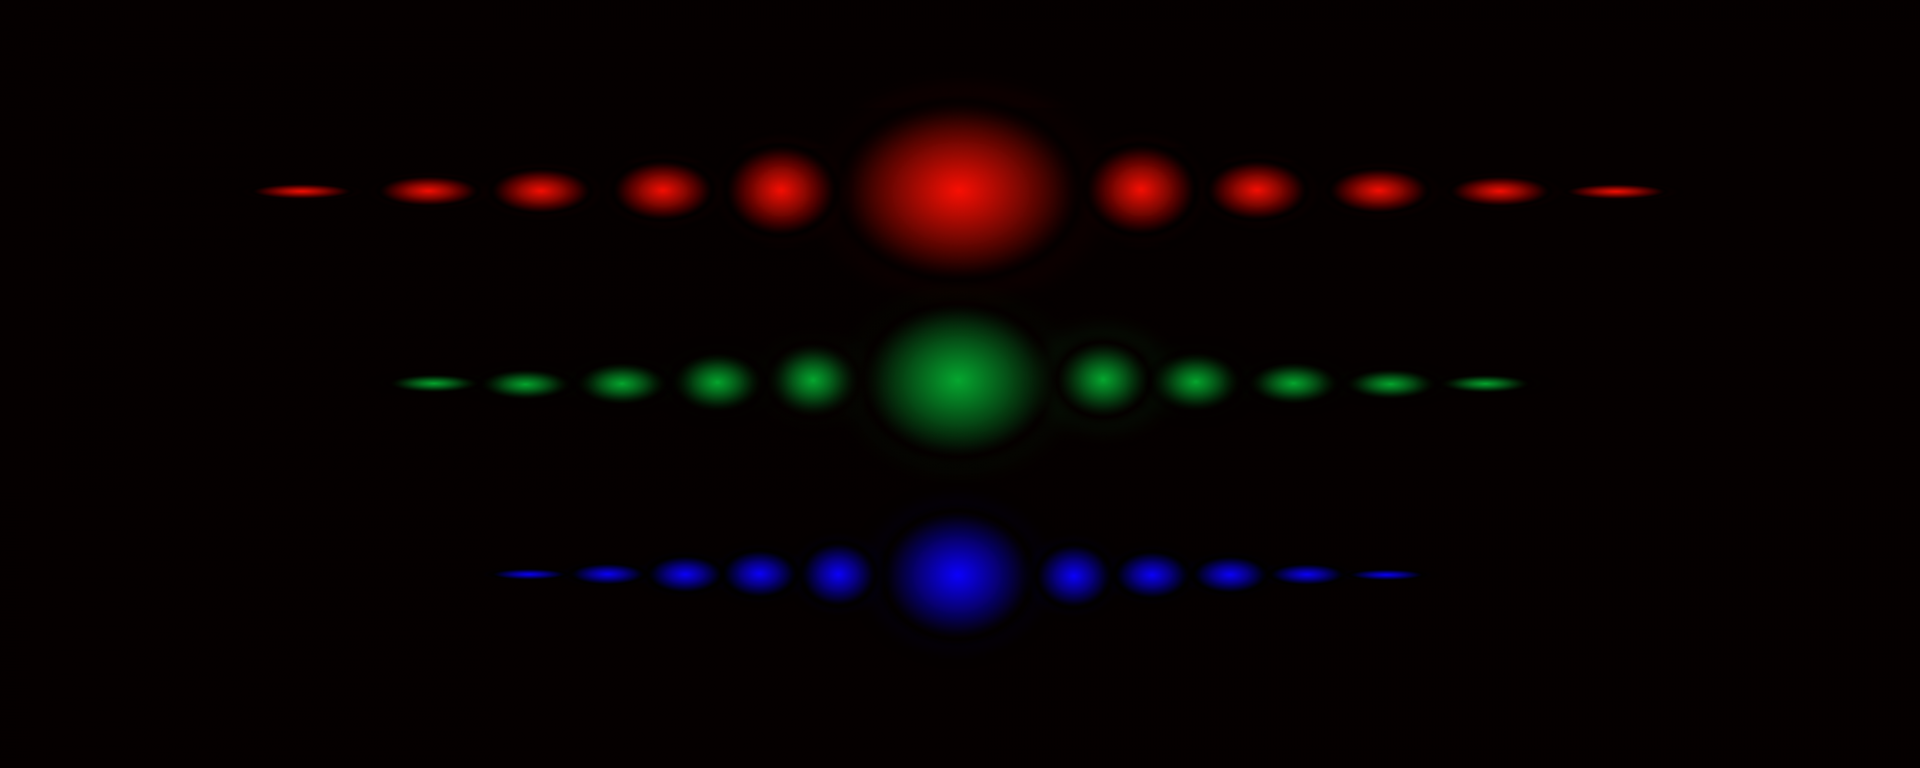
\includegraphics[scale=0.1]{figures/ondes/laser_vert_rouge}
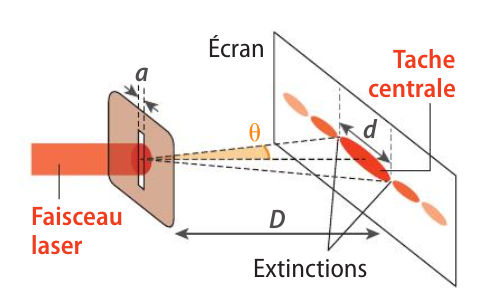
\includegraphics[scale=0.45]{figures/ondes/fig_diff_laser}\\
On place sur le trajet d'un faisceau laser rouge une fente. On réduit peu à peu l'ouverture de la fente.\\
\trou{On observe une alternance de zones lumineuses et sombres. C'est la figure de diffraction.}\\
On remplace le laser rouge ($\lambda = \SI{630}{\nano\meter}$) par un laser vert ($\lambda = \SI{530}{\nano\meter}$). Que constate-t-on ?\\
\trou{On constate que la figure est moins étalée}\\
Quels sont les paramètres influençant la figure de diffraction ?\\
\trou{La largeur de la fente a et la longueur d'onde $\lambda$}\\

}


\etiquette{Application}\\
Parmi les relations suivantes, quelles sont celles qui conviennent après étude des unités ?\\
Quelle est celle qui vous semble conforme aux observations faites ci-dessus ? \\
\begin{center}$\theta=a\times \lambda$ \hspace{2cm}$\theta=\frac{a}{\lambda} $ \hspace{2cm} $\theta=\frac{\lambda}{a}$ \\
\end{center}
\trou{quand a diminue, $\theta$ augmente, et quand $\lambda$ diminue (du rouge au vert), $\theta$ diminue.}
\trou{La relation valable est donc $\theta=\frac{\lambda}{a}$}

\blocrouge{Conclusion}{
\trou{L'écart angulaire $\theta$ est égal à $\frac{\lambda}{a}$ avec $\theta$ en rad, $\lambda$ en m et a en m.}
}


\newpage
\section{Les interférences}

\subsection{Découverte du phénomène}
Considérons un surfeur allongé à l'arrêt sur sa planche. Une vague arrive, le surfeur ne surfe pas, il monte puis redescend et retrouve sa position initiale.\\
Imaginons maintenant qu'une vague arrive d'un côté, et une autre de l'autre côté (peu probable, il est vrai !). deux possibilités : \\
 Les vagues se superposent : Le surfeur monte deux fois plus.
Les vagues s'opposent : Le surfeur ne bouge pas.\\




\verb?http://www.ostralo.net/3_animations/swf/croisement_ondes.swf?\\
Lorsque deux ondes se superposent, leurs élongations s'ajoutent. Deux cas particuliers possibles : \\
\begin{itemize}
\item les deux ondes vibrent en phase

\begin{minipage}{0.5\linewidth}
\centering
\includegraphics[scale=0.3]{figures/ondes/fig2bis}
\end{minipage}
\begin{minipage}{0.5\linewidth}
\centering

\includegraphics{figures/ondes/fig4.pdf}
\end{minipage}
\trou{Dans ce cas, l'amplitude est maximale, on parle d'interférences constructives}
\item les deux ondes sont en opposition de phase\\
\begin{minipage}{0.5\linewidth}
\centering

\includegraphics[scale=0.3]{figures/ondes/fig3}
\end{minipage}
\begin{minipage}{0.5\linewidth}
\centering

\includegraphics{figures/ondes/fig4.pdf}
\end{minipage}
\trou{Dans ce cas, l'amplitude est minimale, on parle d'interférences destructives}
\end{itemize}
C'est ce phénomène qui a lieu dans une cuve à ondes générant deux ondes. Observons-le.\\
\url{https://phet.colorado.edu/sims/html/wave-interference/latest/wave-interference_fr.html}


\vspace{1cm}
\textbf{Analogie pour mieux comprendre :} \\
Imaginons deux personnes qui marchent d'un même pas, des pas de 1m. La longueur d'onde est donc de 2 m pour que le même pied recommence le mouvement.\\
Ces deux personnes doivent poser le pied sur une cible dessinée au sol. On dira que les interférences sont constructives lorsqu'elles posent toutes les deux le même pied, droit ou gauche sur la cible.\\
Elles partent toutes les 2 d'une distance de 4 m, du pied droit, et en même temps.\\
Quel pied vont-elles poser sur la cible ?\\ \trou{Elles vont poser le pied gauche toutes les deux. Interférences constructives.}\\
Maintenant, la personne A ne bouge pas, mais la personne B recule d'un mètre. La personne A a donc 4m à parcourir, mais la personne B doit parcourir 5 m. Quelle est la différence de marche entre les deux personnes, c'est à dire la différence de distance à parcourir ? Que va-t-il se passer ?\\
\vspace{1cm}
\trou{Interférences constructives.}\\

\blocgris{Application}{
\begin{enumerate}
	\item Faire un schéma représentant le chemin parcouru par A et B pour des différences de marche de 2 m, 3 m et 4 m.
	\item Indiquez s'il s'agit d'interférences constructives ou destructives dans chacune des situations. 
	\item Proposez une règle générale pour prédire le type d'interférence à partir de la différence de marche.

\end{enumerate}
}

\vspace{3cm}
En conclusion, on observe que \trou{lorsque la différence de marche est un multiple de $\lambda$, les interférences sont constructives, et que lorsque la différence de marche est un multiple de $\lambda /2$, les interférences sont destructives.}
\\
\blocrouge{Conclusion}{
Dans le cas des interférences constructives : \\
\trou{$\delta= k \times \lambda$ où k est un entier relatif (avec un signe)}\\
Dans le cas des interférences destructives :\\
\trou{$\delta= (k+\frac{1}{2}) \times \lambda$ où k est un entier relatif (avec un signe)}\\
}


\subsection{Interférences lumineuses}

\textbf{cf TP  : Les interférences lumineuses}\\
\etiquette{Vocabulaire} Surligne les mots clés dans le paragraphe suivant:\\
Lorsque deux ondes lumineuses (cohérentes) se superposent, nous observons une figure d'interférences, c'est à dire une alternance de zones brillantes et sombres appelées franges d'interférences.\\
La distance entre 2 franges est appelée interfrange. Elle est notée i. \\
Pour les ondes lumineuses, la différence de marche est aussi appelée différence de chemin optique.

\subsection*{Interférences des trous d'Young : détermination de l'interfrange}

\etiquette{Situation}
Le dispositif des trous d'Young est composé de deux petits trous très proches, ici notés $S_1$ et $S_2$. La distance entre ces trous sera notée b. On éclaire ces trous avec un laser de longueur d'onde $\lambda$, et on place un écran à une distance D très grande devant b.

\begin{minipage}{0.5\linewidth}
\begin{center}
\includegraphics[scale=0.5]{figures/ondes/fig_young.png.pdf}
\end{center}

\end{minipage}
\begin{minipage}{0.5\linewidth}
\begin{center}
\includegraphics[scale=1.3]{figures/ondes/fig_interf}
\end{center}

\end{minipage}


\etiquette{Données du problème}
\begin{itemize}
	\item La longueur d'onde du laser utilisé est égale à $\SI{680}{\nano\meter}$
	\item La distance entre les deux trous, notée b est égale à 0,20 mm.
	\item L'écran sur lequel on observe la figure est placé à 1,20 m des fentes.
\end{itemize}

\etiquetterouge{Objectif} On veut calculer la différence de chemin optique puis l'interfrange $i$ dans le cas d'interférences constructives (puis destructives)
\\
\begin{enumerate}
\item La différence de chemin optique en un point M d'abscisse x est donnée par la relation : \\$\delta=S_2M-S_1M=\dfrac{xb}{D}$ \\

\item Que vaut la différence de chemin optique $\delta$ au centre de la frange centrale ? Est-ce une frange sombre ou lumineuse ?\\
 \trou{$\delta=0$ car le point O est à égale distance des deux sources.}
 
\item Raisonnement avec les franges lumineuses (interférences \trou{constructives}) 
\begin{itemize}
\item Que vaut la différence de chemin optique au centre de la première frange lumineuse ? \trou{$\delta=\lambda$}
\item En déduire la valeur de x au centre de la première frange lumineuse.\\
\trou{$x=\dfrac{\lambda D}{b}$}
\item Sachant que l'interfrange correspond à la distance entre deux franges, déduire la valeur de i.\\
\trou{$i=\dfrac{\lambda D}{b}-0=\dfrac{\lambda D}{b}$}
\end{itemize}

\item Raisonnement avec les franges sombres (interférences \trou{destructives})
\begin{itemize}
\item Que vaut la différence de chemin optique au centre de la première frange sombre ?\\
\trou{$\delta=\dfrac{\lambda}{2}$}
\item En déduire la valeur de x au centre de la première frange sombre ?
\trou{$x=\dfrac{\lambda D}{2b}$}
\item Que vaut la différence de chemin optique au centre de la deuxième frange sombre ?\\
\trou{$\delta=(1+\dfrac{1}{2}) \times \lambda = \dfrac{3\lambda}{2}$}
\item En déduire la valeur de x au centre de la deuxième frange sombre ?\\
\trou{$\dfrac{3\lambda}{2}=\dfrac{xb}{D}$ donc $x=\dfrac{3\lambda D}{2b}$}
\item En déduire la valeur de l'interfrange.\\
\trou{$i=\dfrac{3\lambda D}{2b}-\dfrac{\lambda D}{2b}=\dfrac{2\lambda D}{2b}=\dfrac{\lambda D}{b}$}
\end{itemize}
\item Calculer la valeur de l'interfrange dans les conditions de l'expérience.\\
\trou{$i=\dfrac{\lambda D}{b}=\dfrac{\SI{680e-9}{} \times 1,20}{\SI{0,20e-3}{}}=\SI{4.08e-3}{\meter}=\SI{4.08}{\milli\meter}$}
\end{enumerate}
\underline{remarque }: Pour observer des interférences à partir d'une onde lumineuse il faut créer des sources secondaires à partir de la même source.


\blocrouge{Conclusion}{
Dans une figure d'interférences, les franges brillantes (ou sombres) sont équidistantes. La distance entre 2 franges brillantes (ou sombres) consécutives s'appelle \trou{l'interfrange}. Elle est égale à \trou{$i=\dfrac{\lambda D}{b}$}
}

\etiquette{Exercices} à faire dans votre livre:
\begin{itemize}
\item 2 p 377 ; 
\item 11 p 379 ;
\item  23 p 381 ;
\item  26, 27 p 383 ;
\item Prépa ECE p 385 (à faire absolument pour s'exercer sur la partie diffraction)
\end{itemize}

% \setcounter{chapter}{10}
\chapter{Les lois de Képler}

\section{Un satellite de la Terre}
\subsection{Situation}

On étudie le système Satellite (noté S) de masse $m$ situé à une distance $r$ du centre de la Terre (noté T) et de masse $M_T$. Le référentiel choisit est le référentiel: \trou{géocentrique} considéré galiléen.


\blocrouge{Définition}{le référentiel géocentrique est situé au centre de la Terre et possède trois axes fixes dans l'espace. Il est galiléen.
}

\paragraph*{Bilan des forces} Le système est soumis à la force de gravitation exercée par la Terre sur le satellite. 

\begin{figure}[!htp]
\begin{center}

\includegraphics[height=5cm]{gfx/gravitation}
\end{center}
\caption{Force d'attraction gravitationnelle}
\end{figure}
\subsection{Expression vectorielle de la force gravitationnelle}

On sait que la valeur de la force gravitationnelle subit par le Satellite vaut 
\begin{equation*}
	\boxed{F_{Terre/Satellite}=\trou{\mathcal{G}.\frac{m\times M_T}{r^2}} } 
\end{equation*}

\begin{itemize}
	\item m, $M_T$ les masses des objets en kg
	\item $r$: la distance en m entre les centres des objets
	\item $\mathcal{G}=\SI{6,67e-11}{S.I}$: la constante universelle de gravitation à ne pas confondre avec $g$ l'intensité du champ de pesanteur.
 
\end{itemize}

On doit être capable d'écrire mathématiquement $\overrightarrow{F_{Terre/Satellite}}$. Pour cela on utilise un vecteur unitaire (de norme \trou{égale à 1})que l'on indique sur le schéma. Ici, c'est le vecteur $\overrightarrow{u_{ST}}$  orienté de \trou{ S vers T}. On obtient alors:

$$\overrightarrow{F_{Terre/Satellite}}=\trou{\mathcal{G}.\frac{mM_T}{r^2}\overrightarrow{u_{ST}}}$$
% \marginpar{Cette expression est très souvent demandée en exercice}
\subsection{Expression vectorielle de l'accélération}
Appliquons la seconde de Newton au système satellite:
\begin{eqnarray}
m \overrightarrow{a} && = \overrightarrow{F_{Terre/Satellite}} \nonumber \\
&& = \mathcal{G}.\frac{m.M_T}{r^2}. \overrightarrow{u_{ST}} \nonumber
\end{eqnarray}
En simplifiant par $m$ on trouve l'expression vectorielle du vecteur accélération:


\begin{equation} \overrightarrow{a} =\trou{\mathcal{G}.\frac{M_T}{r^2}.\overrightarrow{u_{ST}}} \label{eq:acc}
\end{equation}

\subsection{Calcul de la vitesse}
\paragraph*{Rappel de cinématique}
Pour un mouvement circulaire quelconque le vecteur accélération $ \overrightarrow{a}$ se décompose en une composante tangentielle $a_T$ et une composante normale $ a_N$ telles que: 
\begin{figure}[!h]
\begin{center}
\includegraphics[scale=0.7]{gfx/mvtcirculaire}
\end{center}
\caption{Composantes du vecteur accélération lors d'un mouvement circulaire}
\end{figure}

\begin{equation}
\overrightarrow{a} =\trou{ \frac{dv}{dt}}. \overrightarrow{T} + \trou{\frac{v^2}{R}} . \overrightarrow{N}
\label{eq:frenet}
\end{equation}

$ \overrightarrow{T}$ et $ \overrightarrow{N}$ sont des vecteurs unitaires (de norme égale à 1) ils sont appelés vecteur Tangentiel et vecteur Normal.

 En comparant les équations \ref{eq:acc} et \ref{eq:frenet} et en constatant que $ \overrightarrow{N}= \overrightarrow{u_{ST}}$, on trouve par identification:
 \begin{eqnarray}
 a_T && = \frac{dv}{dt}= \trou{0} \label{eq:aT}\\
 a_N && = \frac{v^2}{r}=\trou{ \mathcal{G}\frac{M_T}{r^2}} \label{eq:vitesse}
 \end{eqnarray}
De l'équation \ref{eq:aT}, on en déduit que \trou{ $v=cste$} c'est à dire que le mouvement est \trou{uniforme}.
Nous venons de prouver que si le mouvement est \trou{circulaire} alors il est \trou{uniforme}.
%\marginpar {Cette preuve est à savoir faire pour le bac}


A l'aide de l'équation \ref{eq:vitesse}, on isole $v$ et on en déduit la vitesse d'un satellite en mouvement circulaire uniforme dont le rayon de l'orbite est $r$:
\begin{equation}
\boxed{v=\sqrt{\mathcal{G}\frac{M_T}{r}}}
\end{equation}
\etiquette{Conséquence} Plus le satellite est éloigné plus sa vitesse est \trou{petite} (r au dénominateur). Plus l'astre autour duquel il tourne est massif et plus sa vitesse est \trou{grande} ($M_T$ au numérateur)
\subsection{Calcul de la période}
Le mouvement étant circulaire uniforme, S effectue un mouvement périodique autour de la Terre. 

\blocrouge{Définition}{  La durée notée $T$ mise par S pour faire une fois le tour de la Terre, s'appelle la \trou{\textbf{période de révolution}}.}

 
 Puisque la distance parcourue autour de la Terre vaut: $2\pi r$ et que cette distance a été parcourue à une vitesse $v$ pendant une durée $T$, on a:
 
\begin{eqnarray}
T  && =\trou{ \frac{2 \pi r}{v} }\label{eq:periode}\\
T  && = 2\pi \sqrt{\frac{r^3}{\mathcal{G}.M_T}} \label{eq:periodeG}
\end{eqnarray}

\newpage
\blocgris{Application}{On considère l'orbite de la Lune comme étant circulaire de rayon $r=\SI{3.84e5}{\kilo\meter}$. La vitesse de la Lune autour de la Terre est : $v_L=\SI{1.02e3}{\meter\per \second}$

\begin{enumerate}
\item Exprimer, puis calculer la période de révolution $T_L$ de la Lune autour de la Terre. Convertir cette durée en jours.
\item La période de rotation de la Lune sur elle-même est égale à 27,3 jours. Comparer cette période à $T_L$. Quelle est la conséquence de ce résultat ?
\end{enumerate}
}
\vspace{6cm}
\section{Lois de Képler}
\subsection{Référentiel héliocentrique}
Pour décrire le mouvement des planètes autour du Soleil, il est pratique d'affirmer que le Soleil est immobile est que les planètes sont en mouvement autour de lui. Cette description revient à choisir comme référentiel le Soleil, on parle de référentiel \trou{héliocentrique}. Les axes de ce référentiel pointent vers 3 étoiles éloignées (et donc considérées comme fixes). On admettra que ce référentiel est galiléen.

Simulateurs des lois de Képler: 

\url{https://phet.colorado.edu/sims/html/keplers-laws/latest/keplers-laws_all.html}
\\ \url{https://physique.ostralo.net/kepler/}
\subsection{Première loi (1609)}

\blocrouge{Première Loi de Képler}{
Dans le référentiel héliocentrique, la trajectoire du centre de gravité d'une planète est \trou{une ellipse} dont le centre du Soleil est un \trou{Foyer}}
%\marginpar{Les lois de Képler sont à savoir}
\newpage
\subsection{Seconde loi}

\begin{figure}[!htp]
\begin{center}
\includegraphics[height=4cm]{gfx/Loidesaires}

\end{center}
\caption{2nde loi de Képler}
\label{fig:loidesaires}
\end{figure}

\blocrouge{Seconde Loi de Képler}{
Le segment de droite reliant les centres de gravité du Soleil et de la planète balaie \trou{des aires égales pendant des durées égales}.} 


\etiquette{Explications}

 Soit $\Delta t$ une durée (par exemple 1 mois), on a représenté sur la figure \ref{fig:loidesaires} l'aire balayée par le segment reliant le centre de la Terre et le centre du Soleil. Ce segment a décrit une surface\trou{ $A_1$}. 

D'après la 2nde loi de Képler l'aire décrite par ce segment à partir d'un autre instant $t_2$ et pour une même durée $\Delta t$ vaut \trou{$A_2$ } et on a \trou{$A_1=A_2$}.

Or, la distance entre B et C étant plus grande qu'entre D et E cela signifie que la vitesse de la Terre est plus \trou{grande} sur la portion BC que sur la portion DE. Dans ce cas, on prouve que lorsque le mouvement est elliptique, il n'est pas \trou{uniforme}.


\etiquetterouge{Conclusion} La deuxième loi de Képler permet de justifier que la Terre n'a pas toujours la même vitesse au cours de son mouvement autour du Soleil. Sa vitesse est plus \trou{grande} lorsqu'elle est \trou{proche} du Soleil.

\subsection{Troisième loi de Képler(1618)}

\blocrouge{Enoncé }{
Pour toutes les planètes gravitant autour du Soleil à la période T et dont le demi grand axe de la trajectoire vaut a, on a: $$\trou{\frac{T^2}{a^3}=constante}$$
}
\etiquette{Cas particulier important: MCU}

Dans le cas du MCU, le rayon du cercle joue le rôle du demi-grand axe $a$.
On peut alors démontrer la troisième loi de Képler dans le cas particulier de la trajectoire circulaire. Il suffit de mettre au carré l'équation  \ref{eq:periodeG}. 

\begin{eqnarray}
T^2 && =4\pi^2\frac{r^3}{\mathcal{G}.M_T}  \\
\frac{T^2}{r^3} && =\frac{4 \pi^2}{\mathcal{G}.M_T}=cste 
\end{eqnarray}

\etiquetterouge{Les points importants}

Les choses à connaître par coeur:
\begin{itemize}
	\item Les définitions
	\item L'expression vectorielle de la force de gravitation
	\item Les coordonnées du vecteur accélération pour un mouvement circulaire uniforme dans le repère de Frénet
	\item Les 3 lois de Képler + schémas
\end{itemize}

\etiquetterouge{A savoir faire}

\begin{itemize}
	\item Ecrire l'expression vectorielle de la force de gravitation en prenant en compte le sens du vecteur unitaire choisi ou imposé par le texte.
	\item Démontrer que si le mouvement est circulaire alors la vitesse de l'astre (ou satellite) est constante.
	\item Démontrer la troisième loi de Képler dans le cas d'une trajectoire circulaire
\end{itemize}

\blocgris{Sujets de bac pour s'entraîner}{

\begin{itemize}
\item  Polynésie Jour 2 2024 "La masse de la Terre" 
	\item Bac 2024 Centres étrangers 1 Jour 2 EXERCICE 2 : à la découverte des lunes glacées de Jupiter (6 points)
\item Asie 2014
Exercice 1 Le monde selon Hubble (7 points)
\end{itemize}
}
% \setcounter{chapter}{11}
\chapter{Dipôle RC}


\section{Rappels}
\etiquette{Pour commencer}
	Travailler la page 424: carte mentale, réactiver ses connaissances et flash test
	
%	\begin{center}
%	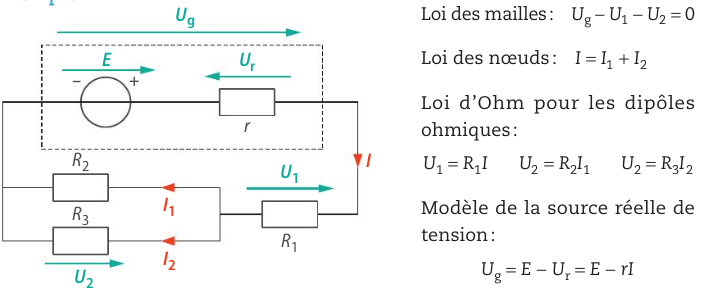
\includegraphics[scale=0.5]{figures/rc/rappels}
%	\end{center}

\section{Courant électrique: débit de charges}
\blocrouge{Définition}{\textbf{En régime permanent, indépendant du temps,} si pendant une durée $\Delta t$ une charge électrique Q traverse une section de conducteur, on définit l'intensité du courant :
\begin{center}
\trou{$I=\dfrac{Q}{\Delta t}$}
\end{center}
\textbf{En régime variable, dépendant du temps,} l'intensité i dépend du temps, on écrit i(t) ou simplement i. L'intensité du courant comme étant un débit de charges électriques. Cela correspond à la charge électrique qui traverserait une section de conducteur durant 1 seconde.  i se calcule en dérivant la fonction $q(t)$:
\begin{center}
\trou{$i(t)=\dfrac{dq}{dt}$}
\end{center}}

\etiquette{Application} Si à chaque seconde, la section d'un fil est traversée par une charge de 3 coulomb cela signifie que $$q(t)= 3\times t$$ on dit alors que l'intensité du courant qui traverse la section du fil vaut :$$i(t)= \trou{\dfrac{d(3t)}{dt	}=3\:A}$$

\section{Le condensateur}
	\subsection{De quoi est fait  un condensateur ?}
	
Un condensateur est composé de deux surfaces conductrices, placées face à face, les armatures. Elles sont séparées par un matériau isolant. \\
le symbole d'un condensateur est le suivant :\\
\begin{center}
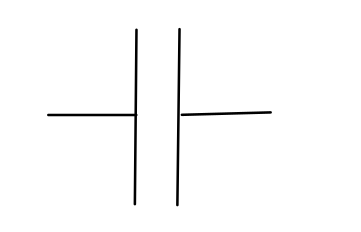
\includegraphics[scale=0.3]{figures/rc/condo}
\end{center} 

	\subsection{Phénomène de charge d'un condensateur}
	
Lorsqu'il est soumis à une tension électrique, le condensateur <<condense>> les charges positives d'une part et négatives d'autre part. Les charges s'accumulent sur \trou{les armatures}.\\
Les deux armatures d'un condensateur portent des charges électrique \trou{opposées}. On dit que le condensateur se \trou{charge}. Dans le même temps, une tension électrique apparaît entre les armatures. On la note \trou{$u_C$}.
\begin{center}
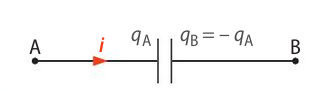
\includegraphics[scale=0.5]{figures/rc/condo2}
 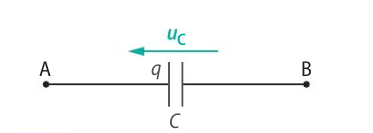
\includegraphics[scale=0.5]{figures/rc/uc}
\end{center}
 L'aptitude d'un condensateur à accumuler sur ses surfaces conductrices un grand nombre de charges électriques est appelée capacité. \\
  La capacité se note C et se mesure en \trou{farad (F)}\\



	\href{https://phet.colorado.edu/sims/html/capacitor-lab-basics/latest/capacitor-lab-basics_en.html}{Simulation condensateur}
	
	
	\subsection{Formules pour le condensateur}
		\begin{center}
					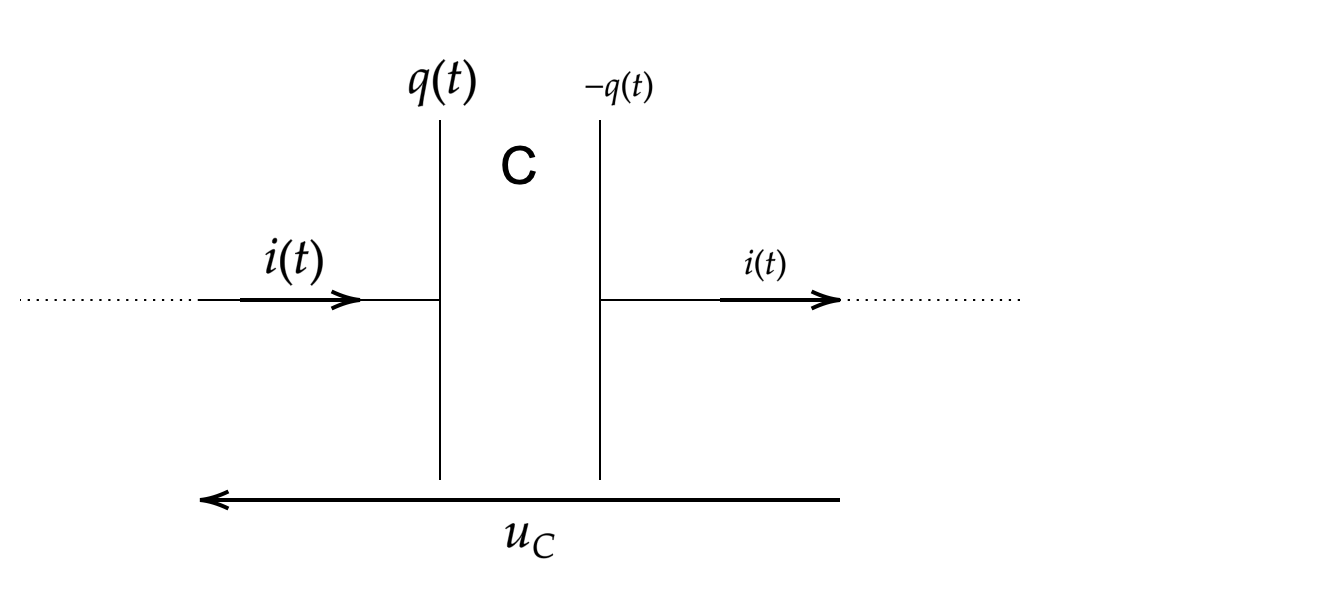
\includegraphics[scale=.18]{figures/rc/rc_resume}
		\end{center}
		\etiquetterouge{Relation Tension - Charge}
		$$\boxed{q=C\times u_C}$$
		$q$ en coulomb (C) ; C en Farad (F) et $u_C$ en volt (V)
			
	\etiquette{Comment la géométrie du condensateur modifie sa capacité ?}
	
	\begin{itemize}
		\item Si on augmente la surface des plaques alors \trou{la capacité du condensateur augmente.}
		\item Si on augmente la distance entre les plaques alors  \trou{la capacité du condensateur diminue.}
	\end{itemize}

	
			\etiquetterouge{Relation Courant - Tension} 
		
		On a vu que $$i(t)=\dfrac{dq}{dt}$$ en remplaçant $q$ par $C\times u_C$ on obtient $$i=\trou{\dfrac{d(C\times u_C)}{dt} }$$ Puisque $C$ est constant, on peut le "sortir" de l'opération de dérivation.

			$$\boxed{\trou{i=C.\dfrac{du_C}{dt}}}$$
	\subsection{Capteurs capacitifs}
Un capteur capacitif utilise les modifications de la capacité d'un condensateur. Ces modifications ont lieu lorsque la distance entre les armatures change, ou lorsque la nature de l'isolant change par exemple.\\
Exemples de capteurs capacitifs :
\begin{itemize}
\item \textbf{Capteur de \trou{ remplissage}} : Pour connaître le niveau de remplissage d'une cuve par exemple, on peut utiliser un capteur capacitif de remplissage. A mesure que le liquide remplit la cuve, l'isolant entre les armatures change (au départ, c'était de l'air, puis lorsque le niveau monte, cela devient le fluide). La capacité évolue donc en fonction de la hauteur de liquide qu'il contient.
\item \textbf{Capteur de \trou{position sur un écran tactile}} : Doc D et E p 429. La surface en verre d'un écran capacitif de smartphone comprend une grille de fils très fins électriquement chargée.\\
lorsqu'un doigt touche l'écran, des charges électriques sont transférées entre le doigt et l'écran, modifiant localement le champ électrique créé par ces fils. La détection de ces variations permet au téléphone de localiser la zone de contact doigt-écran.
\end{itemize}
\newpage

\section{Circuit RC série}  
	\subsection{Décharge d'un condensateur}

\blocgris{Situation}{
\begin{center}
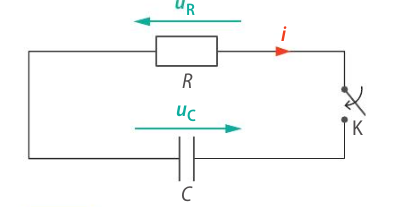
\includegraphics[scale=0.4]{figures/rc/decharge}
\end{center}

On dispose d'un condensateur initialement chargé: $\trou{u_c(t=0)= E}$ (tension E à ses bornes). Le condensateur est branché en série avec un conducteur ohmique de résistance R.\\ A l'instant $t=\SI{0}{\second}$, on ferme l'interrupteur. 
}


\etiquetterouge{Objectif} Trouver l'expression mathématique de la tension \trou{$u_c(t)$} aux bornes du condensateur pendant sa décharge.\\
\etiquette{Stratégie} 
\begin{enumerate}
	\item Appliquer la loi des mailles
	\item Utiliser les formules du condensateur pour écrire une équation différentielle en $u_c(t)$
	\item Résoudre l'équation différentielle en utilisant une condition initiale
\end{enumerate}

\etiquette{Etape 1: loi des mailles}
D'après la loi des mailles dans le circuit, on a :
\begin{center}
$0=\trou{u_c}+\trou{u_R}$ 
\end{center}
\etiquette{Etape 2: formules}
$$u_R=Ri=R\times \trou{C\dfrac{du_c}{dt}}$$
\etiquette{Établissement de l'équation différentielle}\\

On en déduit que :
\begin{center}
$RC\dfrac{du_c}{dt}+u_c=0$\\
\end{center}

et donc \begin{center}
$\dfrac{du_c}{dt}+\dfrac{1}{RC}u_c=0$
\end{center}
ou encore: $$\boxed{\dfrac{du_c}{dt}=-\dfrac{1}{RC}u_c}$$

Il s'agit d'une équation différentielle du premier ordre sans second membre.\\

\blocrouge{Outil Mathématique}{Les solutions d'une équation différentielle $$y'=a\times y +b$$ s'écrivent $$y=K\times e^{\trou{a.x}} - \trou{\frac{b}{a}}$$ avec K une constante à déterminer à l'aide d'une condition initiale. En général, la condition initiale utilise la valeur de y pour  $x=0$.}

\blocgris{Application directe}{ On cherche la fonction y de la variable x telle que $$y'=2y+5$$ avec la condition $y(0)=1$. 

Utilisons l'outil mathématique avec: $a=\trou{2}$, $b=\trou{5}$ la solution s'écrit: $$y=K\times\trou{ e^{2.x}-\frac{5}{2}}$$ il reste à trouver K  en utilisant $y(0)=1$. \\On remplace $x$ par $0$ dans l'expression de $y$ $$y(0)=\trou{K\times e^0-\frac{5}{2}}$$ or on sait que $y(0)=1$ alors $$1=K-\trou{\frac{5}{2}}\quad \text{soit}\quad K=\frac{7}{2}$$
Finalement la solution s'écrit: $$y=\trou{\frac{7}{2}e^{2x}-\frac{5}{2}}$$
}
\newpage
\etiquette{Etape 3: Résolution de l'équation différentielle}\\
On cherche $u_c$ telle que $$\boxed{\dfrac{du_c}{dt}=-\dfrac{1}{RC}u_c}$$ On sait que $u_c(0)=E$ \\E est une valeur connue, c'est la tension initiale du condensateur.
\\
Utilisons l'outil mathématique avec: $a=\trou{-1/RC}$, $b=\trou{0}$ \\
Cette équation a une solution de la forme $u_c(t)=K e^{-t/RC}$.\\
$u_c(0)=E=K$ on en déduit que $K=E$\\
On a donc la solution :
$$\trou{u_c(t)=E\times e^{-t/RC}}$$


\blocrouge{Définition du Temps Caractéristique: $\tau$}{
Le temps $\tau$ qui caractérise la durée de la décharge (ou de la charge) d'un condensateur dans le circuit a pour valeur $$\trou{\tau=R\times C}$$ $\tau$ est en seconde (s) ; $C$ en F et R en ohm ($\Omega$)
}

\etiquette{Comment déterminer $\tau$ ?}\\
\begin{center}
	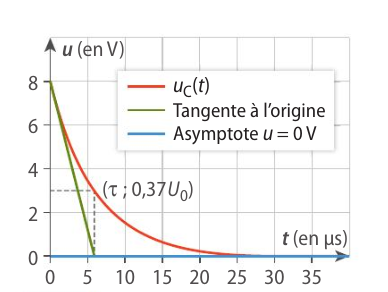
\includegraphics[scale=0.65]{figures/rc/tau_decharge}	
\end{center}


\textbf{Première méthode }:\\
Calculons $u_c(\tau)$ : $u_c(\tau)=Ee^{-\tau/\tau}=\trou{0,37}\times E$\\
Afin de déterminer $\tau$, il suffit donc de tracer la droite d'équation $u=0,37.E$ et de lire l'abscisse du point d'intersection de cette droite avec la courbe représentant $u_c$ pendant la décharge.\\
\textbf{Deuxième méthode : }\\
On trace la tangente à l'origine. Cette tangente coupe l'axe \trou{des abscisses}  à la date t=$\tau$.




		\subsection{Etude de la charge}
 	
 	\blocgris{Situation}{
 
Un condensateur est monté en série avec un dipôle ohmique de résistance R et une source de tension E.
L'interrupteur est initialement ouvert, on le ferme au temps t=0s.\\
On étudie les variations de la tension $u_c$ au cours du temps.
\\
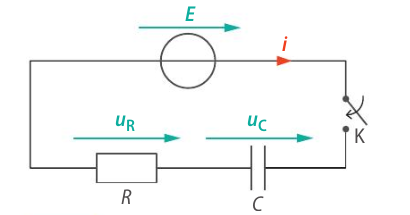
\includegraphics[scale=0.5]{figures/rc/circuit_charge}
}

\etiquetterouge{Objectif} Trouver l'expression mathématique de la tension $u_c(t)$ aux bornes du condensateur pendant sa charge.\\


\etiquette{Etape 1}
D'après la loi des mailles dans le circuit, on a :
\begin{center}
$\trou{E}=u_c+u_R$ 
\end{center}
\etiquette{Etape 2}
$$u_R=Ri=\trou{RC\dfrac{du_c}{dt}}$$
On en déduit que :
\begin{center}
$RC . \trou{\dfrac{du_c}{dt}}+\trou{u_c}=E$\\
\end{center}

et donc en divisant tous les termes par $RC$ 
$$\dfrac{du_c}{dt}+\dfrac{1}{RC}.u_c=\dfrac{E}{RC}$$
On ordonne les termes afin d'obtenir la forme $y' = ay + b$
$$\boxed{\dfrac{du_c}{dt}=-\dfrac{1}{RC}.u_c+\dfrac{E}{RC}}$$
Comme pour la décharge, il s'agit d'une équation différentielle du premier ordre. Résoudre cette équation c'est trouver la fonction $u_c(t)$.

\etiquette{Résolution de l'équation différentielle}

On cherche $u_c(t)$ telle que $$\boxed{\dfrac{du_c}{dt}=-\dfrac{1}{RC}.u_c+\dfrac{E}{RC}}$$ avec $$u_c(t=0)= 0\:V \quad\text{condition initiale}$$

Utilisons l'outil mathématique avec: $a=\trou{-1/RC}$, $b=\trou{\frac{E}{RC}}$ soit $-\frac{b}{a}=E$ (à vérifier vous même!!)\\
Cette équation a une solution de la forme $u_c(t)=\trou{K e^{-t/RC}+E}$\\
Déterminons K, en utilisant $$u_c(0)=0\quad\text{et aussi}\quad u_c(0)=Ke^0+E$$ donc $$K=\trou{-E}\quad\Rightarrow u_c(t)=\trou{-E.e^{-t/RC}} + \trou{E}$$ En factorisant par E: $$\boxed{u_c(t)=E\times \left( 1- e^{-t/RC}\right)}$$
	 
\etiquette{Représentation graphique de $u_c(t)$}\\
\begin{center}
	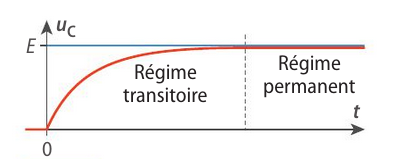
\includegraphics[width=0.4\textwidth]{figures/rc/courbe_charge}	
	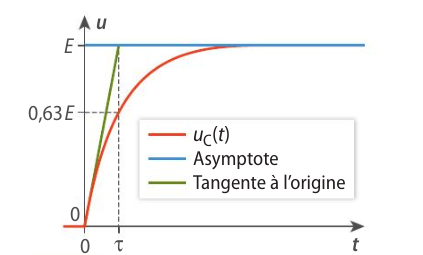
\includegraphics[width=0.6\textwidth]{figures/rc/tau}
\end{center}

\paragraph*{Observations} 
\begin{itemize}
	\item On constate qu'après une certaine durée, la tension du condensateur n'évolue plus. On dit que le régime \trou{transitoire} est terminé et que le régime \trou{permanent} est atteint.  
	\item Après $5\times \tau$ l'écart entre $u_c(t)$ et son asymptote est de moins de 1 \%.
\end{itemize}

\etiquette{Détermination de $\tau$}
\textbf{Première méthode }:\\
Calculons $u_c(\tau)$ : $u_c(\tau)=E(1-e^{-\tau/\tau})=E(1-e^{-1})=0,63E$\\
Afin de déterminer $\tau$, il suffit donc de tracer la droite d'équation $u=0,63E$ et de lire l'abscisse du point d'intersection de cette droite avec la courbe représentant $u_c$ pendant la charge.\\
\textbf{Deuxième méthode : }\\
On trace la tangente à l'origine. Cette tangente coupe l'asymptote $u_c=E$ à la date t=$\tau$.

	 
	\section*{Exercices à faire}
A partir de la page \textbf{434} et suivantes \\
\begin{itemize}
	\item Restituer le cours: 3, 4, 10, 11	 
	\item Etablir l'équation différentielle: 12, 13
	\item Résoudre l'équation différentielle: 15, 16
	\item Mesure de $\tau$: 18
	\item Synthèse: Lire les bons réflexes p 434 - Faire et étudier en détail l'ex1 p 434 
	\item S'entraîner pour le contrôle 19, 21
	\item Préparer le BAC: 30	 
	

\end{itemize}

Un sujet de bac: Amérique du nord 2021 Sujet 1 Exercice 1 Partie B

 \url{https://labolycee.org/un-sport-traditionnel-le-lancer-de-gerbe-de-paille}
	 
	 
% \setcounter{chapter}{11}
\chapter{Cinétique Chimique}

\section{Rappels de 1ère sur l'oxydoréduction}
\subsection{Oxydant/Réducteur}
\begin{itemize}
	\item Un oxydant est une espèce chimique capable de \trou{capter} un ou plusieurs électrons.
	\item Un réducteur est une espèce chimique capable de \trou{céder} un ou plusieurs électrons.
	\item De manière générale on peut écrire cet échange sous la forme d'une demi-équation électronique: $$\boxed{Ox + n\cdot e^- = Red}$$
\end{itemize}
\etiquette{Exemples} $Cu^{2+}/Cu$ ; $I_2/I^-$ ; $H^+/H_2$ sont des couples redox. Ecrire les demi-équations électroniques associées à chaque couple.
\begin{align*}
	Cu^{2+} + \trou{2e-} &= Cu\\
I_2 + \trou{2e^-} &= \trou{2I^-}\\
\trou{2H^+} +\trou{ 2e^-} &= \trou{H_2}
\end{align*}

\blocrouge{Méthodes pour écrire les demi-équations}{
\begin{enumerate}
	\item Equilibrer les atomes autres que\trou{ O et H}.
	\item Equilibrer O en ajoutant des \trou{molécules d'eau}.
	\item Equilibrer H en ajoutant des ions \trou{$H^+$}.
	\item Ajouter des électrons pour \trou{équilibrer les charges électriques}
\end{enumerate}}

\etiquette{Application} Ecrire les demi-équations électroniques associées aux couples suivant: $O_2/H_2O$ ; $H_2O_2/H_2O$ ; $O_2/H_2O_2$ ; $MnO_4^-/Mn^{2+}$.
\newpage
\subsection{Equation chimique d'une réaction d'oxydoréduction}
\blocrouge{Méthode} {
\begin{enumerate}
	\item Repérer les couples.
	\item Ecrire les demi-équations dans le sens où elles se font (voir exemple) 
	\item Vérifier que chaque demi-équation échange le même nombre d'électrons. Si ce n'est pas le cas, multiplier par des coefficients appropriés.
	\item Additionner les demi-équations. Les électrons doivent se neutraliser.
	\item Vérifier que l'équation obtenue est équilibrée en termes d'atomes et de charges.
\end{enumerate}
}

\etiquette{Exemples} On fait réagir le fer Fe et le dichlore $C\ell_2$. Voici les couples redox: $Fe^{3+}/Fe$ et $C\ell_2 / C\ell^-$.
\begin{align*}
 \trou{ 2\text{Fe}} &\rightarrow \trou{2\text{Fe}^{3+}} +\trou{ 6e^-} \\
    \trou{3}\text{Cl}_2 + \trou{6}e^- &\rightarrow \trou{6\text{Cl}^- }\\
    \hline
    \trou{2\text{Fe} + 3\text{Cl}_2 }&\rightarrow \trou{2\text{Fe}^{3+} + 6\text{Cl}^-}
\end{align*}


\section{Transformations lentes et rapides}
\subsection{Transformations rapides}
\etiquette{Critère}
Une transformation est rapide lorsque à nos yeux elle semble instantanée. C'est à dire que les réactifs se transforment en produits en moins d'une seconde.

\etiquette{Exemples:}
\begin{itemize}
	\item Les explosions sont des réactions très rapides.
	\item Les réactions qui forment des précipités sont très rapides. \\
Réaction entre les ions chlorures et les ions argents pour former le chlorure d'argent

\end{itemize}

Schéma + équation de la réaction

\vspace{3cm}

\subsection{Transformations lentes}
Les réactions qui ne sont pas rapides sont lentes...

\etiquette{Exemple}

coucher de soleil du chimiste

\subsection{Comment suivre l'évolution des réactions lentes ?}

\etiquette{Problème} Comment mesurer la quantité de matière de produit apparu à chaque instant pendant que la réaction se fait ?

\etiquetterouge{3 techniques à relier aux TP}
\begin{enumerate}
	\item Si le produit ou le réactif est coloré: on suit l'absorbance avec un spectrophotomètre.
	\item Si le produit ou un réactif est un ion: on suit la conductivité avec un conductimètre.
	\item On prélève un échantillon du milieu réactionnel et on effectue un titrage. (voir chapitre Titrages)	
\end{enumerate}

\section{Comment modifier la vitesse d'une réaction ?}
\subsection{Facteurs cinétiques}

\blocrouge{Définitions}{
\begin{itemize}
	\item Un facteur cinétique est une grandeur qui a une influence sur la durée de la réaction chimique.
	\item Il existe 2 facteurs cinétiques: 
		\begin{enumerate}
			\item \trou{La température: Plus la température est élevée plus la réaction est rapide.}
			\item \trou{La concentration: Plus la concentration des réactifs est grande plus la réaction est rapide.}
		\end{enumerate}
\end{itemize}
}
\subsection{Mise en évidence expérimentale}
Voir TP Facteurs Cinétiques


\subsection{Catalyser une réaction}
\blocrouge{Définition}{
Un catalyseur est une espèce chimique qui diminue la durée d'une transformation chimique. Il ne modifie pas \trou{l'état final du système}.
}

\etiquette{Conséquences et propriétés}
\begin{itemize}
	\item Un catalyseur ne figure pas dans l'équation chimique de la réaction.
	\item La quantité de produit formé ne dépend pas de la présence d'un catalyseur.
	\item Le catalyseur n'est pas \trou{consommé} et se retrouve intégralement à la \trou{ fin } de la réaction.
	\item Un catalyseur est en général spécifique à une réaction chimique.
\end{itemize}

\etiquette{Effet de la présence d'un catalyseur}
L'eau oxygénée réagit sur elle même car l'eau oxygénée est à la fois un oxydant et un réducteur. 

Les couples oxydant/réducteur impliqués sont :
\begin{align*}
    \text{O}_2 / \text{H}_2\text{O}_2 \\
    \text{H}_2\text{O}_2 / \text{H}_2\text{O}
\end{align*}

Écrire les Demi-Équations d'Oxydoréduction :

Pour \(\text{O}_2 / \text{H}_2\text{O}_2\) (réduction) :
\begin{align*}
   \text{H}_2\text{O}_2 &=  \text{O}_2 + \trou{2\text{H}^+} + \trou{2}e^-
\end{align*}

Pour \(\text{H}_2\text{O}_2 / \text{H}_2\text{O}\) (oxydation) :
\begin{align*}
    \text{H}_2\text{O}_2 +\trou{ 2\text{H}^+} +\trou{ 2e^-} &= \trou{2}\text{H}_2\text{O} 
\end{align*}

En additionnant membre à membre, on obtient la réaction de Dismutation de l'eau oxygénée: $$2H_2O_2 \longrightarrow 2H_2O + O_2 $$
Différentes catalyses possibles pour cette réaction :
\begin{enumerate}
	\item utilisation de Pt (catalyse hétérogène)
	\item solution de $Fe^{2+}$ (catalyse homogène)
\end{enumerate}


%\newpage
\section{Vitesse volumique}
\subsection{Situation}
La réaction entre les ions peroxodisulfate $S_2O_8^{2-}$ et les ions iodures $I^-$ est lente. Elle produit du diiode (orange) et des ions sulfate incolore selon:
$$S_2O_8^{2-}+2I^-\longrightarrow 2 SO_4^{2-}+I_2$$ 
\begin{minipage}{0,45\linewidth}
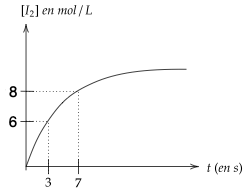
\includegraphics[scale=1]{figures/cinetique/fig_cinetique1_v2}
\end{minipage}
\begin{minipage}{0,6\linewidth}

Ci-contre, la courbe d'évolution de la concentration du diiode dans le mélange réactionnel au cours du temps.\\
Le diiode étant une espèce colorée, cette courbe a pu être obtenue par spectrophotométrie.
\end{minipage}

\etiquette{Estimation de la vitesse volumique d'apparition de $I_2$}
\begin{itemize}
	\item Entre t=3 s et t=7 s il s'est écoulé une durée de \trou{7-3 = 4 s}.
	\item Pendant cette durée, la concentration du diiode a augmenté de: \trou{10-8=2 mol/L}
	\item On peut donc dire qu'en 4 s la concentration a augmenté de 2 mol/L.
	\item Cela correspond à une vitesse volumique moyenne de $$V_{app}(I_2) \approx \frac{2 \: mol/L}{4\:s}=0,5\:mol.L^{-1}.s^{-1}$$
\end{itemize}

\etiquetterouge{Attention} Nous allons maintenant calculer la vitesse volumique instantanée en reprenant l'idée de vitesse instantanée vue en mécanique. C'est cette définition et la technique qui suit que vous devez retenir.
\subsection{Généralisation et définition rigoureuse de la vitesse volumique}
\includegraphics{figures/cinetique/fig_cinetique2}


$$V_{app}(X)=\dfrac{[X](t+\Delta t)-[X](t)}{\Delta t}$$

Si $\Delta t$ tend vers 0, alors la vitesse d'apparition moyenne tend vers la vitesse d'apparition instantanée.
$$\lim\limits_{\Delta t \to 0}V_{app}(X)=\lim\limits_{\Delta t \to 0}\dfrac{[X](t+\Delta t)-[X](t)}{\Delta t}$$
\blocrouge{Définition de la vitesse volumique d'apparition}{On note $[X](t)$ la concentration d'un produit $X$ à l'instant t, dans le mélange réactionnel. Entre les instants $t$ et $t+\Delta t$ la concentration de $X$ augmente. Pour rendre compte de la vitesse la concentration de $X$ augmente, on calcule sa vitesse volumique d'apparition :$$V_{app}(X)=\trou{\frac{d[X]}{dt}}$$
\begin{itemize}
	\item $[X]$ est la concentration en mol/L
	\item t le temps en s
	\item $V_{app}$ en $mol.L^{-1}.s^{-1}$
\end{itemize}}

\newpage
\subsection{Technique pour calculer une vitesse volumique d'apparition}

\blocrouge{Technique}{La vitesse volumique d'apparition est égale \trou{au coefficient directeur de la tangente à la courbe. }}

\etiquette{Exemple}

\begin{minipage}{0,45\linewidth}
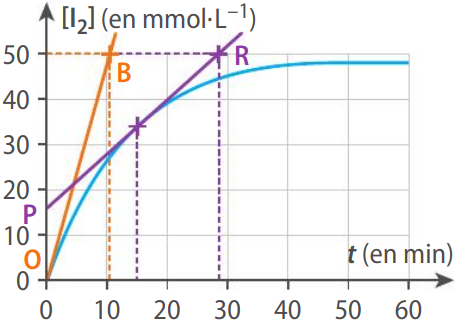
\includegraphics[scale=0.5]{figures/cinetique/fig_3}
\end{minipage}
\begin{minipage}{0,45\linewidth}
Déterminer les vitesses volumiques d'apparition de $I_2$ au temps t=0 et au temps t=15 min. Commenter.
\end{minipage}

\vspace{8cm}
\subsection{Vitesse volumique de disparition}
Soit R un réactif dont on souhaite connaître la vitesse de disparition. En utilisant le même raisonnement que pour la vitesse d'apparition, on va calculer s'intéresser à la dérivée de sa concentration $\dfrac{d[R]}{dt}$.

La vitesse de disparition est positive.  $[R](t)$ est décroissante donc sa dérivée est négative. C'est pourquoi, on ajoute un signe - pour le calcul de la vitesse de disparition.

\blocrouge{Définition}{
Soit $X$ un réactif consommé lors d'une réaction, sa vitesse volumique de disparition est donnée par
$$V_{disp}(X)=-\frac{d[X]}{dt}$$
\begin{itemize}
	\item $[X]$ est la concentration en mol/L
	\item t le temps en s
	\item $V_{disp}$ en $mol.L^{-1}.s^{-1}$
\end{itemize}}
 
 
\section{Loi de vitesse d'ordre 1}
\subsection{Contexte}
Considérons une réaction ayant pour équation :
\begin{center}
$ a A + b B \longrightarrow c C$
\end{center}
La vitesse de disparition du réactif A s'écrit alors : $$V_{disp}(A)=\trou{-\dfrac{d[A]}{dt}}$$


\blocrouge{Définition}{
Une réaction chimique suit une loi de vitesse d'ordre 1 si à tout instant t, la vitesse volumique de disparition est proportionnelle à la concentration en A, c'est à dire si :\\
$$V_{disp}(A)=\trou{k[A](t)=-\dfrac{d[A]}{dt}}$$ où $k$ est une constante.
}


\etiquette{Unités}
Retrouver par analyse dimensionnelle l'unité de k.\\
\vspace{2cm}

\etiquette{Aspect mathématique: Equation différentielle}
Lorsque la loi de vitesse est d'ordre 1: et donc : $$\trou{\dfrac{d[A]}{dt}+k[A](t)=0}$$ On montre (voir annexe) que l'évolution au cours du temps de la concentration de A suit une loi exponentielle décroissante qui s'écrit: $$[A](t) = [A]_0 \times e^{-k.t}$$
\newpage
\section{Temps de demi-réaction}

\blocrouge{Définition}{
Le temps de demi réaction $t_{1/2}$ est la durée au bout de laquelle l'avancement $x(t_{1/2})$ la réaction a atteint  la moitié de la valeur de l'avancement final $x_f$. $$x(t_{1/2})=\frac{x_f}{2}$$
}

\etiquette{Détermination Graphique}

\begin{minipage}{0,45\linewidth}
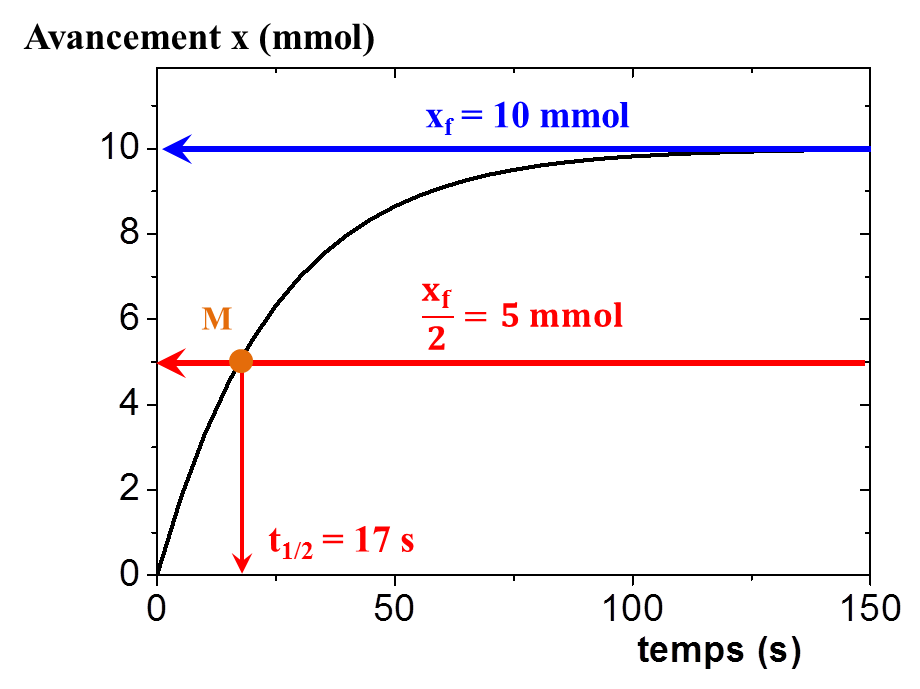
\includegraphics[scale=.5]{figures/cinetique/demi_reaction.png} 
\end{minipage}
\begin{minipage}{0,45\linewidth}
Technique: Repérer la valeur de l'avancement maximal, calculer $x_f /2$. Trouver le point de la courbe dont l'ordonnée est $x_f /2$. Son abscisse est le temps de demi-réaction
\end{minipage}

Autre type de graphique: Représentation de la concentration d'un réactif au cours du temps ou de l'absorbance d'un réactif au cours du temps.

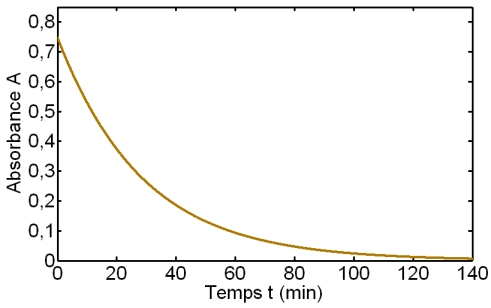
\includegraphics[scale=.45]{figures/cinetique/fig_4.jpg}


\section{Comment tester si une loi de vitesse est d'ordre 1 ?}
\subsection{3 Techniques à connaître}
\etiquette{Technique 1: En utilisant t1/2}\\
On réalise plusieurs expériences en faisant varier les concentrations initiales $[A]_0$. Si le temps de demi-réaction ne change pas d'une expérience à une autre alors la loi de vitesse est d'ordre 1.Faire \textbf{Ex 11 p 86}

\etiquette{Technique 2: Vitesse proportionnelle à la concentration}

Si la vitesse de disparition d'une réactif est proportionnelle à la concentration de ce réactif $$V_{disp}(A)=\trou{k[A](t)}$$ Alors la loi de vitesse est d'ordre 1. \textbf{Ex 13 p 86} (estimer les vitesses à partir des cordes de la courbe)

\etiquette{Technique 3: Modélisation de l'évolution de $[A](t)$}

Pour une loi de vitesse d'ordre 1, on a $[A](t)=[A]_0e^{-kt}$.\\ On peut vérifier cette relation par une modélisation de $[A(t)]$ en utilisant Regressi ou un programme Python. 

Voir \textbf{2022-Centres Etrangers-J1-ExoC-Sujet-Cinetique-AcBase}


\section*{ANNEXES}
\subsection*{Annexe 1: Solution de l'équation différentielle}
Résolution de $\dfrac{d[A]}{dt}= -k[A](t)$
On reconnaît une équation différentielle d'ordre 1. 

\etiquette{Solution Générale}

$[A](t)=Ce^{-k\cdot t}$ où  C une constante est solution de l'équation différentielle.

Vérifiez que c'est bien le cas en injectant cette expression dans l'équation différentielle.

\etiquette{Recherche de C avec une condition initiale}

On sait que à t=0 
\begin{itemize}
	\item la concentration en A est connue: $[A](t=0) = [A]_0$ 
	\item en utilisant la solution générale, on a aussi: $[A](t=0) = C.e^{-k\times 0} = C$
\end{itemize}
Donc $$C =  [A]_0$$
Connaissant $C$, nous pouvons réécrire la solution générale de manière complète.

\etiquette{Conclusion}
$$\boxed{[A](t) = [A]_0 \times e^{-k.t}}$$

\subsection*{Annexe 2}
On prend le logarithme de $[A(t)]$ ce qui donne : \trou{$ln([A](t))=ln([A]_0)-kt$}\\

En traçant le graphe de \trou{ln[A] en fonction du temps}

\subsection*{Interprétation du graphique}
\begin{center}
	\includegraphics[scale=.8]{figures/cinetique/loi_vitesse} 
\end{center}
2 cas possibles: 
\begin{enumerate}
	\item On obtient une droite de coefficient directeur égal à -k : la loi de vitesse est d'ordre 1.
	\item On n'obtient pas une droite, alors l'évolution de la concentration ne suit pas une loi de vitesse d'ordre 1. 	
\end{enumerate}


\blocrouge{A FAIRE}{
\begin{itemize}
	\item Résumé et techniques + quizz: \url{https://youtu.be/NO87Hcyt7OU}
	\item  6,13,14,15,19, 22 et prépa ece p90
	\item  Sujet type BAC: Centres étrangers 2021 sujet 2
\end{itemize}}




 
 %\newpage
 \section{Modélisation microscopique}
 \subsection{Acte élémentaire}
\blocrouge{Définition}{
A l'échelle microscopique, on observe une réaction se déroulant en \trou{une seule étape} $$A+B\longrightarrow C+D$$ cette réaction est appelée \trou{acte élémentaire}.
}


\etiquette{Choc efficace ?}

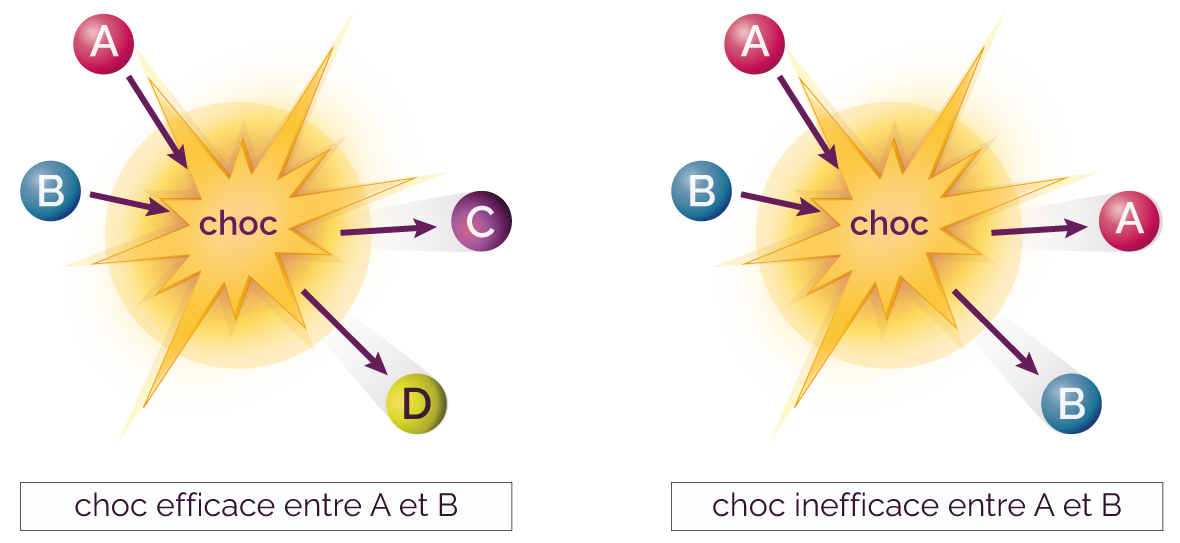
\includegraphics[width=10cm]{figures/cinetique/choc.png}

La simple rencontre des réactifs A et B ne suffit pas à engendrer l'apparition des produits.  Cette rencontre doit se faire sous la forme d'une choc suffisamment violent pour que les liaisons chimiques de A et B se réorganisent pour former les produits C et D. On dit que le choc est \trou{efficace}.

\etiquette{Conséquences}

\begin{itemize}
	\item Plus la température est grande, plus l'efficacité des chocs est \trou{grande} et plus la vitesse de réaction est \trou{grande}.
	\item Plus la concentration d'un réactif est grande, plus les chocs efficaces sont \trou{fréquents}et plus la vitesse est grande.
\end{itemize}
 
\subsection{Mécanisme Réactionnel}
\blocrouge{Définition}{Une réaction chimique peut être décomposée en une \trou{succession d'actes élémentaires}. Cette décomposition forme un \trou{mécanisme réactionnel}.}
 
 \etiquette{Exemple} La réaction entre le chlorométhane et l'ion hydroxyde s'écrit à l'échelle macroscopique: $$CH_3-C\ell + HO^- \longrightarrow CH_3-OH + C\ell^-$$
 Son mécanisme réactionnel, comporte deux actes élémentaires :
 

\begin{alignat*}{2}
    &\textbf{Acte élémentaire 1} \quad \quad \quad &&CH_3-Cl \leftrightharpoons CH_3-C^+ + Cl^- \\
    &\textbf{Acte élémentaire 2} \quad \quad \quad &&CH_3-C^+ + HO^- \leftrightharpoons CH_3-OH \\
    \hline 
    &\textbf{Bilan} \quad &&\trou{CH_3-Cl + HO^- \longrightarrow CH_3-OH + Cl^-}
\end{alignat*}

\blocrouge{Intermédiaire Réactionnel}{Un intermédiaire réactionnel est une espèce chimique qui \trou{apparaît dans un acte élémentaire} et disparaît dans l'acte suivant. Il ne figure pas dans le bilan de la réaction.}

\etiquette{Travail} Repérer dans le mécanisme ci-dessus un intermédiaire réactionnel.

\blocrouge{Repérer un catalyseur !}{Dans un mécanisme réactionnel, le catalyseur est présent dans l'acte 1 et régénéré dans un acte suivant. La présence du catalyseur modifie le mécanisme réactionnel.}

La réaction précédente est maintenant réalisée en présence d'ion iodure $I^-$. Voici le mécanisme réactionnel: 

\begin{alignat*}{2}
    &\textbf{Acte élémentaire 1} \quad \quad \quad &&CH_3-Cl + I^-\leftrightharpoons CH_3-I + Cl^- \\
    &\textbf{Acte élémentaire 2} \quad \quad \quad &&CH_3-C^+ + HO^- \leftrightharpoons CH_3-OH + I^-
    \end{alignat*}

\etiquette{Question}
\begin{enumerate}
	\item Justifier que $I^-$ est un catalyseur
	\item Justifier que la présence du catalyseur ne modifie pas l'équation bilan de la réaction.
\end{enumerate}

\etiquetterouge{Conclusion} L'équation bilan d'une réaction modélise à l'échelle macroscopique la réaction chimique. Le mécanisme réactionnel donne une modélisation microscopique dont les actes élémentaires peuvent mettre en évidence un ou plusieurs intermédiaires réactionnels.
En faisant la somme  des actes élémentaires on retrouve \trou{l'équation bilan.}

\newpage
\section{Formalisme de la flèche courbe}
	\subsection{A quoi ça sert ?}

Afin de justifier les actes élémentaires, on utilise des flèches courbes pour montrer le déplacement des doublets électroniques. La flèche est toujours orientée du site donneur vers le site accepteur de doublet. Elle s'écrit du doublet vers l'atome (cf exemple). La ou les flèches courbes sont toujours côté réactif dans l'acte élémentaire.

\etiquette{Exemple}

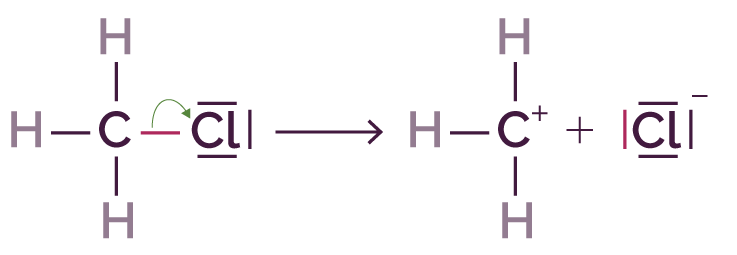
\includegraphics[width=8cm]{figures/cinetique/fleche1.png}

\subsection{Site donneur / Site accepteur}
\etiquette{Site Donneur}

\begin{enumerate}
	\item Atome possédant un doublet liant (cf le C de l'exemple)
	\item Atome possédant un \trou{doublet non liant}
\end{enumerate}

\etiquette{Site Accepteur}
\begin{enumerate}
	\item Atome ou ion possédant une lacune (comme l'ion $H^+$ ou l'atome de bore $B$).
	\item Atome possédant une charge formelle.
	\item  Atome avec une charge partielle (liaison polarisée)
\end{enumerate}

\etiquette{Extrait BAC 2018 Afrique}

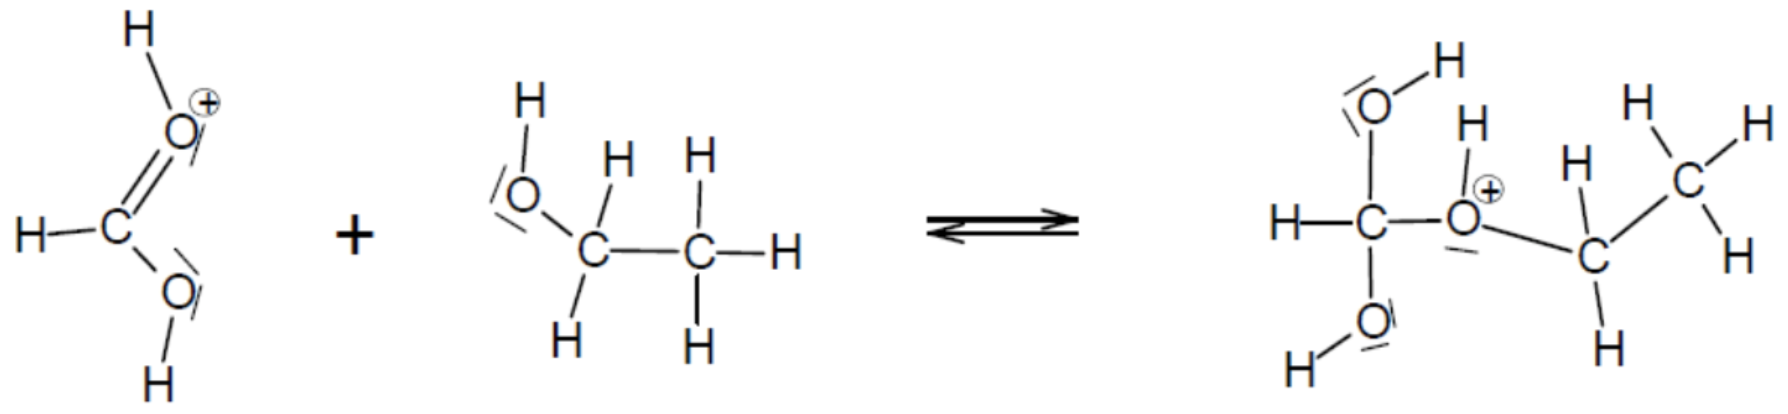
\includegraphics[width=13 cm]{figures/cinetique/sites.png}
 \begin{enumerate}
 	\item Identifier les sites donneurs et le site accepteur mis en jeu lors de l'acte élémentaire.
 	\item Représenter par des flèches courbes les déplacements de doublets électroniques.
 \end{enumerate}
 
 \etiquette{Application directe}
 
 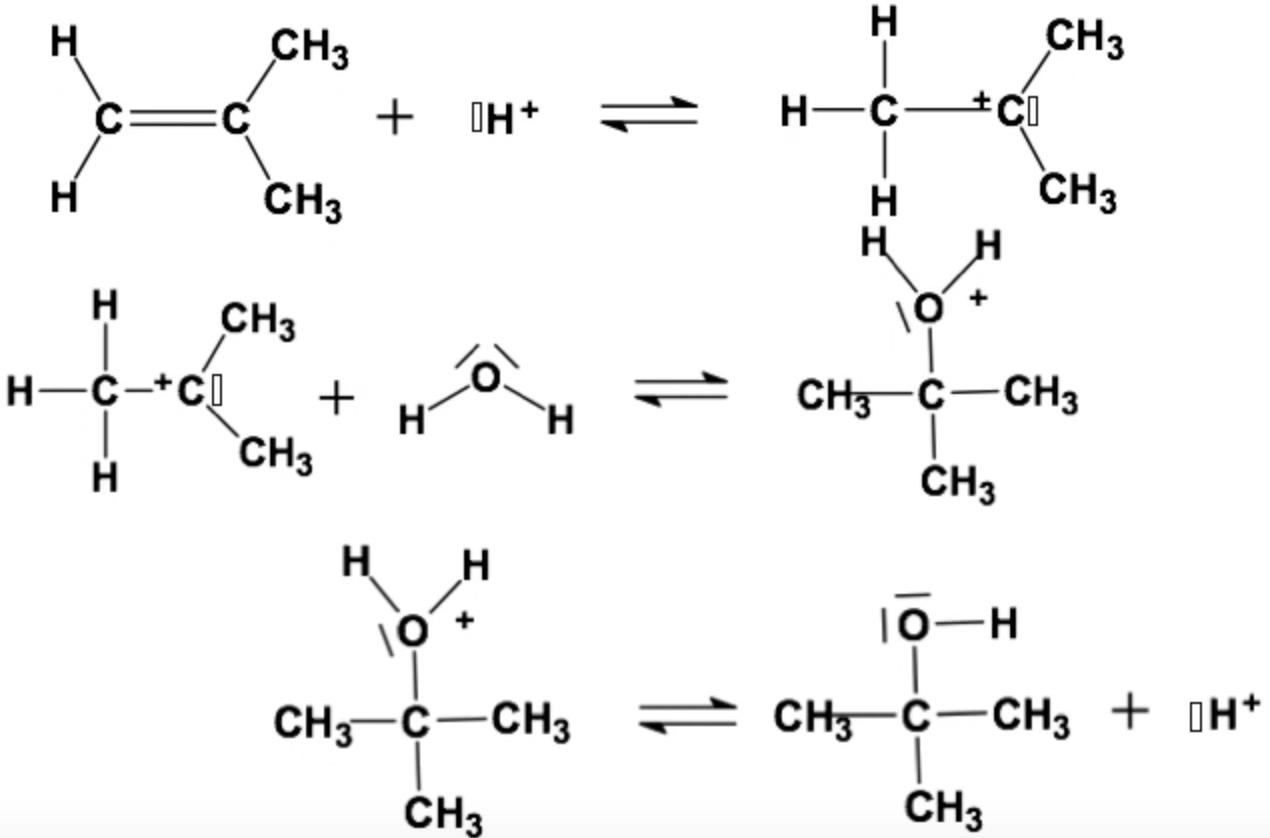
\includegraphics[width=12cm]{figures/cinetique/mecanisme.png}
 
 \begin{enumerate}
 	\item Retrouver l'équation de la réaction modélisée par le mécanisme réactionnel fourni.
 	\item Identifier les intermédiaires réactionnels.
 	\item Quel est le rôle de l'ion hydrogène dans ce mécanisme ? Justifier votre réponse.
 	\item Pour chaque acte élémentaire, représenter les flèches courbes.
 \end{enumerate}

 \etiquette{EXERCICES à faire}
  Dans ton livre: 
  \begin{itemize}
  	\item Vérifier vos réflexes: 5, 7 , 9 p 103
  	\item Pour s'entrainer et faire les classiques: 11 ou 12 p 105 ; 19 p 107
  	\item Muscler son jeu: 20, 21 p 108
  \end{itemize}
 \etiquette{Vidéo}
 Pour revoir en détail l'électronégativité et le déplacement de doublet: 
 \url{https://youtu.be/ETVjaxuNWn8?si=dI-H-Vo9Lh_SBK4E}
% \setcounter{chapter}{13}
\chapter{Radioactivité}

\section{Vocabulaire et rappels}
\subsection{Rappels}

\blocrouge{A savoir}{
	\begin{itemize}
		\item Le noyau d'un atome est formé de protons et de \trou{neutrons}.
		\item Un élément est défini par son numéro atomique Z (c'est le nombre \trou{de protons}) et son symbole chimique.	
		\item Le nombre de masse est noté: A . Il correspond aux nombres de \trou{nucléons} présents dans le noyau (nombre de \trou{protons} + \trou{nombre de neutrons}
		\item La notation symbolique d'un noyau  X est $$_Z^A X$$
		\item Deux noyaux possédant le même numéro atomique mais un nombre de masse différent sont appelés \trou{isotopes}.
	\end{itemize}

}

\etiquette{Application} On considère 3 noyaux: $_{40}^{93}Zr$ ; $_{238}^{92}U$ ; $_{40}^{95}Zr$. 
\begin{enumerate}
	\item Faire l'inventaire des particules contenues dans ces noyaux.
	\item Quels sont ceux qui sont isotopes ? Justifier.
\end{enumerate}

\vspace{4cm}

\subsection{Transformation nucléaire}

La physique nucléaire étudie les propriétés des noyaux des atomes. On observe que certains noyaux peuvent modifier leur composition. Ainsi le nombre de protons et de neutrons est modifié (selon certaines règles...). Ces modifications s'appellent des transformations nucléaires ou encore radioactivité.

\etiquette{Radioactivité alpha}

Une particule $\alpha$ est le nom donné au noyau d'hélium formé de\trou{ 2 protons et 2 neutrons}. 

Exemple de transformation: $$_{94}^{238}Pu \longrightarrow _{2}^{4}He + _{92}^{234}U$$

\blocrouge{Lois de conservation}{Toutes les transformations nucléaires valident 2 lois de conservation:
	\begin{enumerate}
		\item Conservation du nombre de charge 
		\item Conservation du nombre de masse
	\end{enumerate}

}

\etiquette{Radioactivité beta}
Il existe deux types de radioactivité bêta selon que la particule émise est chargée positivement ou négativement.
\begin{itemize}
	\item Radioactivité $\beta^-$ émission d'un électron: $_{-1}^{0}e$. Transformation d'un \trou{neutron} en proton. 
	\item Radioactivité $\beta^+$ émission d'un positron ou positon: $_{+1}^{0}e$. Transformation d'un \trou{proton en neutron}. 
\end{itemize}

\etiquette{Exemples}
\begin{itemize}
	\item Identifier le type de radioactivité
	\item Compléter les transformations chimiques
\end{itemize}

 $$^{238}_{92}U \longrightarrow ^{\trou{234}}_{90}Th + ^{4}_{\trou{2}}He$$

   $$^{11}_{6}C \longrightarrow ^{\trou{11}}_{\trou{5}}B + e^+
$$
  $$^{14}_{7}N \longrightarrow ^{14}_{6}C + \trou{e^- }$$
  
     \subsection{Diagramme (N,Z)}
     
    Sur un diagramme, on repère un noyau par son nombre de protons Z (en abscisse) et son nombre de neutron N (en ordonnée).
    
    Le diagramme complet: \url{https://segree.web-labosims.org/index.html}

    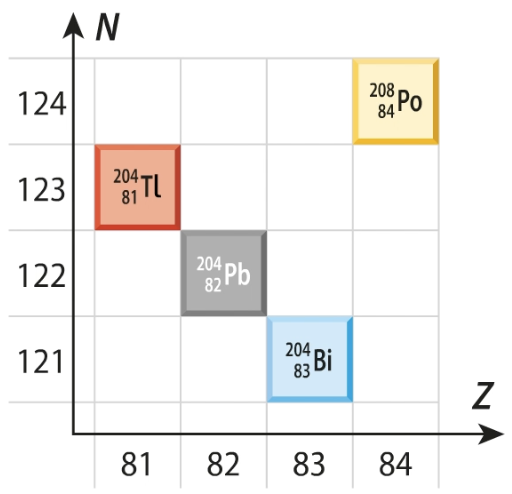
\includegraphics[width=.5\textwidth]{figures/diagramme_NZ}
    
    Les éléments qui ont la même abscisse sont \trou{isotopes}.
    \etiquette{Diagramme et radioactivité} Indiquer par une flèche sur le diagramme les transformations qui mènent les noyaux représentés au plomb.
    Pour chaque transformation, nommer le type de radioactivité.
    
    
\section{Evolution temporelle d'un échantillon radioactif}
\subsection{Cadre et objectif}
On modélise un échantillon de matière radioactive par une collection de noyaux radioactifs. On note $N(t)$ le nombre de ces noyaux. Au cours du temps, de manière \trou{aléatoire} chaque noyau va se désintégrer (et donner naissance à d'autres noyaux) ainsi $N(t)$ décroît au cours du temps. On veut connaître l'expression de  $N(t)$ en fonction de $t$. (voir TP)

\subsection{Activité d'un échantillon radioactif}

\blocrouge{Définition}{L'activité d'un échantillon est égale au nombre de noyaux qui se désintègrent \trou{par seconde}. Elle se note $A(t)$ et s'exprime en \trou{Becquerel} de symbole Bq.}

\etiquette{Démonstration} Preuve que $A(t)=-\frac{dN(t)}{dt}$
\begin{itemize}
	\item A t=0 s, on dispose d'un échantillon contenant $N_0$ noyaux radioactifs.
	\item A l'instant t>0, on veut estimer le nombre de noyaux qui se désintègrent par seconde: $A(t)$.
	\item On peut estimer $A(t)$ en raisonnant sur une durée $\Delta t$ alors: $$A(t)\approx \frac{N(t)-N(t+\Delta t)}{\Delta t}=-\frac{\trou{N(t+\Delta t)-N(t)}}{\Delta t}$$
	\item  Faisons tendre $\Delta t$ vers 0 pour estimer plus \trou{précisément} $A(t)$
	\item On reconnaît la limite d'un taux d'accroissement, on a donc $$A(t)=-\frac{dN(t)}{dt}$$
\end{itemize}

\subsection{Interprétation Graphique}
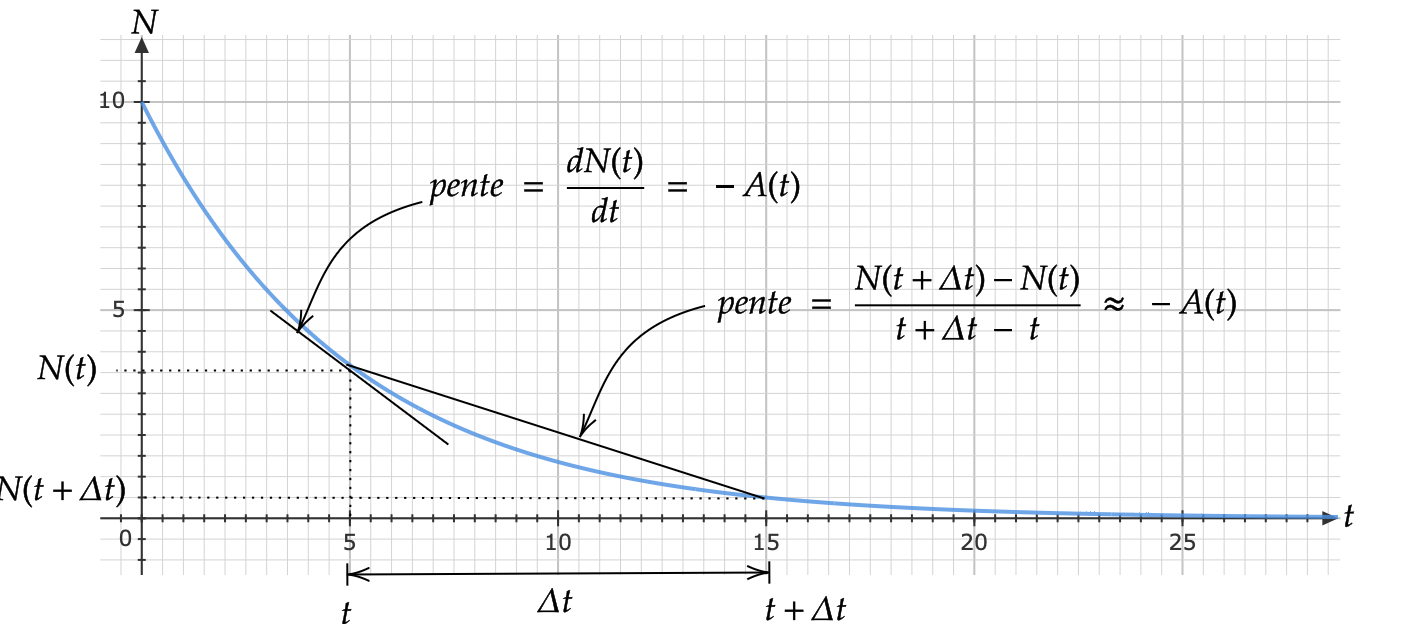
\includegraphics[width=.9\textwidth]{figures/decroissance}

L'activité à l'instant t s'obtient graphiquement en déterminant la \trou{pente} de la \trou{tangente} à la courbe N(t) à l'instant t. Analogue à la vitesse de disparition en chimie.

\subsection{Equation différentielle}

\etiquette{Propriété} On admet que l'activité $A(t)$ est \trou{proportionnelle} au nombre de noyaux radioactifs présents $N(t)$. Ce qui s'écrit $$A(t)=\lambda\times \trou{N(t)}$$


$\lambda$ est appelée la constante radioactive, sa valeur dépend du noyau considéré. Son unité est \trou{la seconde}.
\etiquette{Recherche de N(t)}

En utilisant la définition de $A(t)$ et la propriété ci-dessus on a $$\frac{dN(t)}{dt}=- \lambda \cdot N(t)$$

La solution générale s'écrit: $$N(t)=K\times e^{\trou{-\lambda t}}$$
Calcul de K à l'aide d'une condition initiale, on sait que $N(t=0\:s) = N_0$
$$N(0)=K\times e^0 = N_0 \Rightarrow K=\trou{N_0}$$
\blocrouge{A retenir}{ A tout instant $t\geqslant 0$, $$N(t)=\trou{N_0\times e^{-\lambda t}}$$}


On obtient $A(t)$ par dérivation $$A(t)= -\frac{dN(t)}{dt}=\lambda N_0 e^{-\lambda t}$$

\blocrouge{A retenir}{ A tout instant $t\geqslant 0$, $$A(t)=\trou{A_0\times e^{-\lambda t}}$$ avec $A_0=\lambda N_0$}

\subsection{Conséquences}
Le nombre de noyaux radioactifs et l'activité d'un échantillon décroissent exponentiellement. Le temps caractéristique de cette décroissance est appelé \trou{la demi-vie} (analogue au temps de demi-réaction en chimie)

\etiquette{Exercice} On dispose d'un échantillon contenant à t=0 $N_0$ noyaux radioactifs. Au bout de combien de temps, la moitié de ces noyaux se seront désintégrés.
\vspace{5cm}
\blocrouge{Définition}{La demi-vie est la durée au bout de laquelle la moitié des noyaux radioactifs d'un échantillon se sont désintégrés. Elle se note $t_{1/2}$ et s'exprime en seconde. On a la relation: $$t_{1/2}=\trou{\frac{\ln 2}{\lambda}}$$ }

\etiquette{Exercice} Représenter graphiquement l'allure de $N(t)$ et indiquer comment on détermine $t_{1/2}$

\newpage
\etiquetterouge{Résumé}

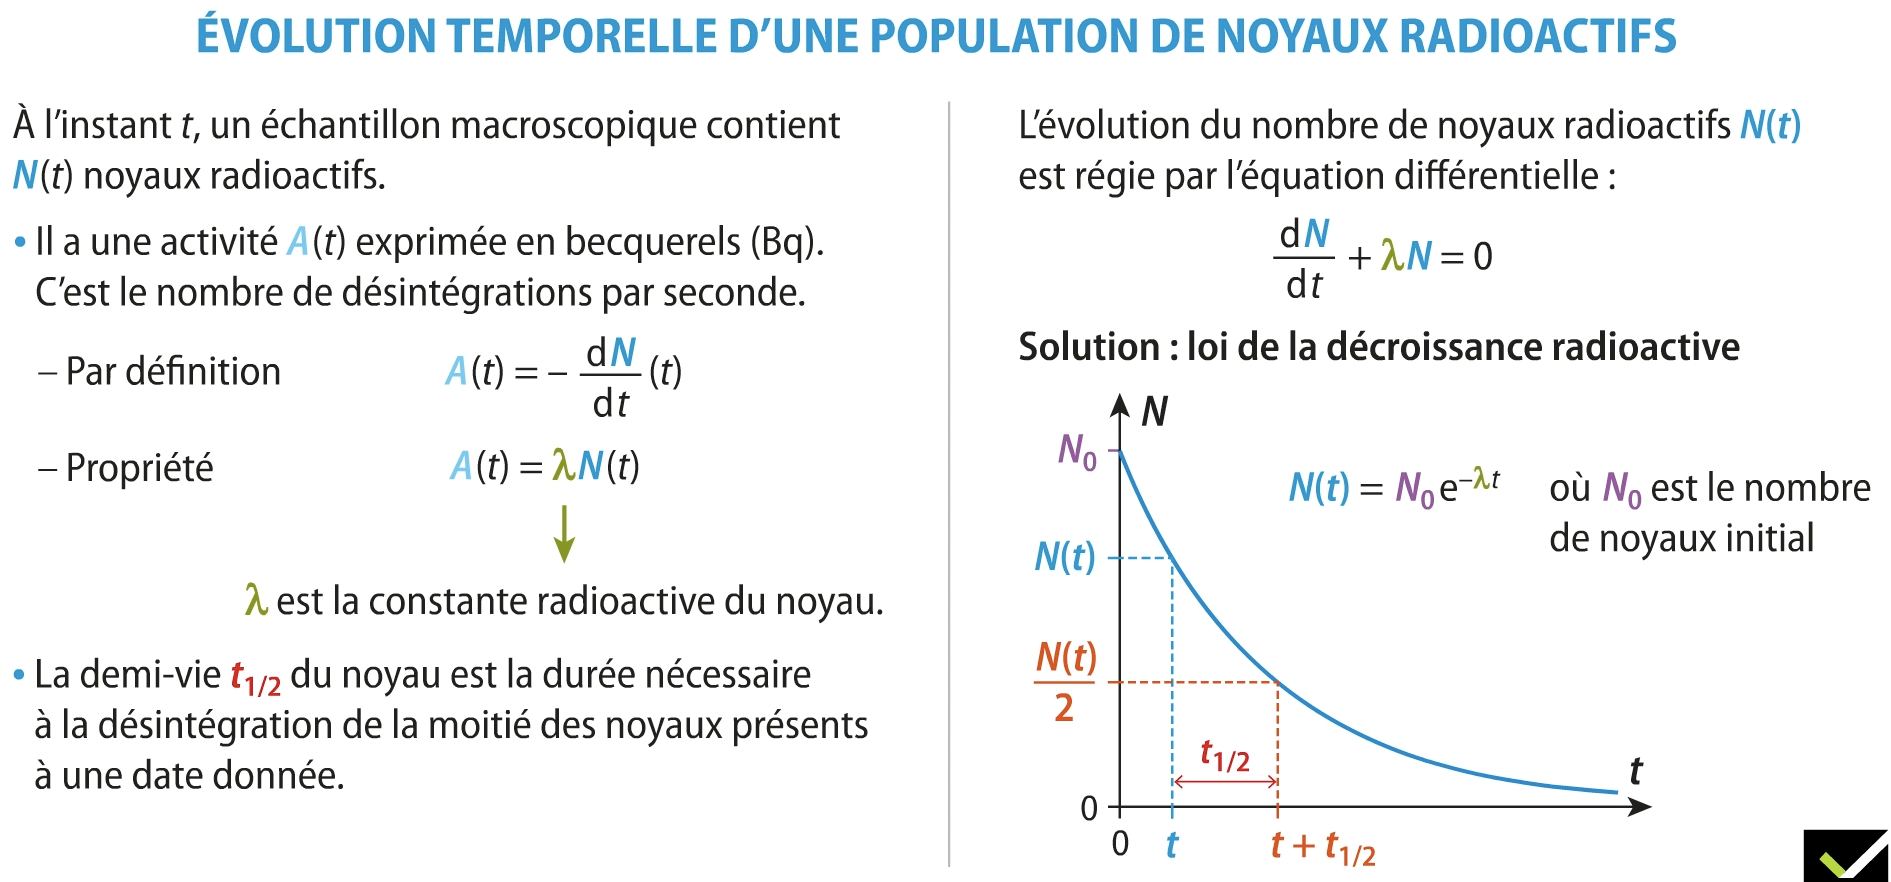
\includegraphics[width=.99\textwidth]{figures/nucleaire_resume.png}
\etiquetterouge{Exercices}

\begin{itemize}
	\item 6 , 12 p 122-123
	\item 19 p 124
	\item 27 et 32 p 126-128
\end{itemize}



% \setcounter{chapter}{14}
\chapter{Mécanique des fluides}

Dans toute cette leçon, le fluide est \trou{incompressible}. Sa masse volumique $\rho$ est une \trou{constante}. Elle ne dépend ni du point du fluide considéré ni du temps.
\section{Equilibre d'un fluide et d'un objet immergé}
\subsection{Statique des fluides (rappels)}

A chaque point M d'un fluide, on peut associer une pression P qui se mesure en \trou{pascal} (Pa).
Sous l'effet du champ de pesanteur $\overrightarrow{g}$, la pression d'un point  du fluide dépend de \trou{son altitude $z$}.

\etiquetterouge{On retient que}

\begin{minipage}{0.45\textwidth}
 $$\boxed{P_2- P_1 =\trou{ \rho g (z_1 - z_2)}}$$
 
 
Attention à \trou{l'orientation} de l'axe (Oz)
\end{minipage}
\hfill
\begin{minipage}{0.45\textwidth}
% Pattern Info
 
\tikzset{
pattern size/.store in=\mcSize, 
pattern size = 5pt,
pattern thickness/.store in=\mcThickness, 
pattern thickness = 0.3pt,
pattern radius/.store in=\mcRadius, 
pattern radius = 1pt}
\makeatletter
\pgfutil@ifundefined{pgf@pattern@name@_3ta6xpmll}{
\pgfdeclarepatternformonly[\mcThickness,\mcSize]{_3ta6xpmll}
{\pgfqpoint{0pt}{0pt}}
{\pgfpoint{\mcSize+\mcThickness}{\mcSize+\mcThickness}}
{\pgfpoint{\mcSize}{\mcSize}}
{
\pgfsetcolor{\tikz@pattern@color}
\pgfsetlinewidth{\mcThickness}
\pgfpathmoveto{\pgfqpoint{0pt}{0pt}}
\pgfpathlineto{\pgfpoint{\mcSize+\mcThickness}{\mcSize+\mcThickness}}
\pgfusepath{stroke}
}}
\makeatother
\tikzset{every picture/.style={line width=0.75pt}} %set default line width to 0.75pt        

\begin{tikzpicture}[x=0.75pt,y=0.75pt,yscale=-1,xscale=1]
%uncomment if require: \path (0,300); %set diagram left start at 0, and has height of 300

%Straight Lines [id:da1431580915407349] 
\draw    (100,280) -- (100,52) ;
\draw [shift={(100,50)}, rotate = 90] [color={rgb, 255:red, 0; green, 0; blue, 0 }  ][line width=0.75]    (10.93,-3.29) .. controls (6.95,-1.4) and (3.31,-0.3) .. (0,0) .. controls (3.31,0.3) and (6.95,1.4) .. (10.93,3.29)   ;
%Straight Lines [id:da19553928863883396] 
\draw    (90,250) -- (110,250) ;
%Straight Lines [id:da945394404180156] 
\draw    (90,120) -- (110,120) ;
%Straight Lines [id:da8594674598946904] 
\draw    (144,119.7) -- (157.4,119.7) ;
%Straight Lines [id:da7274688509203905] 
\draw    (150.7,127.2) -- (150.7,112.2) ;

%Straight Lines [id:da47087832586595935] 
\draw    (194.6,249.5) -- (208,249.5) ;
%Straight Lines [id:da7468781295482437] 
\draw    (201.3,257) -- (201.3,242) ;

%Straight Lines [id:da8920415703778027] 
\draw    (263.6,98.6) -- (263.6,155.4) ;
\draw [shift={(263.6,157.4)}, rotate = 270] [color={rgb, 255:red, 0; green, 0; blue, 0 }  ][line width=0.75]    (10.93,-3.29) .. controls (6.95,-1.4) and (3.31,-0.3) .. (0,0) .. controls (3.31,0.3) and (6.95,1.4) .. (10.93,3.29)   ;
%Shape: Rectangle [id:dp3919081166661982] 
\draw  [pattern=_3ta6xpmll,pattern size=19.799999999999997pt,pattern thickness=0.75pt,pattern radius=0pt, pattern color={rgb, 255:red, 0; green, 0; blue, 0}] (103.6,68.6) -- (309.8,68.6) -- (309.8,294.2) -- (103.6,294.2) -- cycle ;

% Text Node
\draw (95.8,30.4) node [anchor=north west][inner sep=0.75pt]    {$z$};
% Text Node
\draw (68.8,108.4) node [anchor=north west][inner sep=0.75pt]    {$z_{1}$};
% Text Node
\draw (68,238.8) node [anchor=north west][inner sep=0.75pt]    {$z_{2}$};
% Text Node
\draw (159.6,111.8) node [anchor=north west][inner sep=0.75pt]    {$M_{1}$};
% Text Node
\draw (211.2,240.8) node [anchor=north west][inner sep=0.75pt]    {$M_{2}$};
% Text Node
\draw (270.4,114) node [anchor=north west][inner sep=0.75pt]    {$\vec{g}$};
% Text Node
\draw (133.2,273.4) node [anchor=north west][inner sep=0.75pt]   [align=left] {fluide à l'équilibre};


\end{tikzpicture}
\end{minipage}

\subsection{Solide totalement immergé dans un liquide}


\begin{minipage}{0.45\textwidth}
	
\tikzset{every picture/.style={line width=0.75pt}} %set default line width to 0.75pt        

\begin{tikzpicture}[x=0.75pt,y=0.75pt,yscale=-1,xscale=1]
%uncomment if require: \path (0,300); %set diagram left start at 0, and has height of 300

%Straight Lines [id:da1431580915407349] 
\draw    (100,290) -- (100,36) ;
\draw [shift={(100,34)}, rotate = 90] [color={rgb, 255:red, 0; green, 0; blue, 0 }  ][line width=0.75]    (10.93,-3.29) .. controls (6.95,-1.4) and (3.31,-0.3) .. (0,0) .. controls (3.31,0.3) and (6.95,1.4) .. (10.93,3.29)   ;
%Straight Lines [id:da19553928863883396] 
\draw    (90,263.6) -- (110,263.6) ;
%Straight Lines [id:da945394404180156] 
\draw    (90,94) -- (110,94) ;
%Straight Lines [id:da8920415703778027] 
\draw    (323.6,87.1) -- (323.6,143.9) ;
\draw [shift={(323.6,145.9)}, rotate = 270] [color={rgb, 255:red, 0; green, 0; blue, 0 }  ][line width=0.75]    (10.93,-3.29) .. controls (6.95,-1.4) and (3.31,-0.3) .. (0,0) .. controls (3.31,0.3) and (6.95,1.4) .. (10.93,3.29)   ;
%Shape: Rectangle [id:dp5373877667432289] 
\draw   (170,94) -- (280,94) -- (280,264) -- (170,264) -- cycle ;
%Straight Lines [id:da9508886392388277] 
\draw    (170,104) -- (188,104) ;
\draw [shift={(190,104)}, rotate = 180] [color={rgb, 255:red, 0; green, 0; blue, 0 }  ][line width=0.75]    (10.93,-3.29) .. controls (6.95,-1.4) and (3.31,-0.3) .. (0,0) .. controls (3.31,0.3) and (6.95,1.4) .. (10.93,3.29)   ;
%Straight Lines [id:da39799050739514663] 
\draw    (170,174) -- (198,174) ;
\draw [shift={(200,174)}, rotate = 180] [color={rgb, 255:red, 0; green, 0; blue, 0 }  ][line width=0.75]    (10.93,-3.29) .. controls (6.95,-1.4) and (3.31,-0.3) .. (0,0) .. controls (3.31,0.3) and (6.95,1.4) .. (10.93,3.29)   ;
%Straight Lines [id:da6014552387688628] 
\draw    (170,234) -- (208,234) ;
\draw [shift={(210,234)}, rotate = 180] [color={rgb, 255:red, 0; green, 0; blue, 0 }  ][line width=0.75]    (10.93,-3.29) .. controls (6.95,-1.4) and (3.31,-0.3) .. (0,0) .. controls (3.31,0.3) and (6.95,1.4) .. (10.93,3.29)   ;
%Straight Lines [id:da5653486083787891] 
\draw    (262,104) -- (280,104) ;
\draw [shift={(260,104)}, rotate = 0] [color={rgb, 255:red, 0; green, 0; blue, 0 }  ][line width=0.75]    (10.93,-3.29) .. controls (6.95,-1.4) and (3.31,-0.3) .. (0,0) .. controls (3.31,0.3) and (6.95,1.4) .. (10.93,3.29)   ;
%Straight Lines [id:da9278285507191912] 
\draw    (252,174) -- (280,174) ;
\draw [shift={(250,174)}, rotate = 0] [color={rgb, 255:red, 0; green, 0; blue, 0 }  ][line width=0.75]    (10.93,-3.29) .. controls (6.95,-1.4) and (3.31,-0.3) .. (0,0) .. controls (3.31,0.3) and (6.95,1.4) .. (10.93,3.29)   ;
%Straight Lines [id:da2529721799410396] 
\draw    (242,234) -- (280,234) ;
\draw [shift={(240,234)}, rotate = 0] [color={rgb, 255:red, 0; green, 0; blue, 0 }  ][line width=0.75]    (10.93,-3.29) .. controls (6.95,-1.4) and (3.31,-0.3) .. (0,0) .. controls (3.31,0.3) and (6.95,1.4) .. (10.93,3.29)   ;
%Straight Lines [id:da7895068034344014] 
\draw    (230,264) -- (230,216) ;
\draw [shift={(230,214)}, rotate = 90] [color={rgb, 255:red, 0; green, 0; blue, 0 }  ][line width=0.75]    (10.93,-3.29) .. controls (6.95,-1.4) and (3.31,-0.3) .. (0,0) .. controls (3.31,0.3) and (6.95,1.4) .. (10.93,3.29)   ;
%Straight Lines [id:da20361196168232487] 
\draw    (230,94) -- (230,112) ;
\draw [shift={(230,114)}, rotate = 270] [color={rgb, 255:red, 0; green, 0; blue, 0 }  ][line width=0.75]    (10.93,-3.29) .. controls (6.95,-1.4) and (3.31,-0.3) .. (0,0) .. controls (3.31,0.3) and (6.95,1.4) .. (10.93,3.29)   ;

% Text Node
\draw (95.8,14.4) node [anchor=north west][inner sep=0.75pt]    {$z$};
% Text Node
\draw (71,82.4) node [anchor=north west][inner sep=0.75pt]    {$z_{2}$};
% Text Node
\draw (68,252.4) node [anchor=north west][inner sep=0.75pt]    {$z_{1}$};
% Text Node
\draw (330.4,102.5) node [anchor=north west][inner sep=0.75pt]    {$\vec{g}$};
% Text Node
\draw (221,266.4) node [anchor=north west][inner sep=0.75pt]    {$\overrightarrow{F_{1}}$};
% Text Node
\draw (221,64.4) node [anchor=north west][inner sep=0.75pt]    {$\overrightarrow{F_{2}}$};


\end{tikzpicture}
\end{minipage}
\hfill
\begin{minipage}{0.45\textwidth}

Le système étudié est une boite immergée dans un fluide de masse volumique $\rho$. Le fluide exerce des forces de pression sur le système. 
Les forces de pression latérales s'\trou{équilibrent}. La force de pression sur la face supérieure $\overrightarrow{F_2}$ est plus faible que la force de pression qui s'exerce sur la face inférieure $\overrightarrow{F_1}$.

La résultante des forces de pression s'écrit: $$\trou{\overrightarrow{F_1}+\overrightarrow{F_2}}= \overrightarrow{F_p}$$
$\overrightarrow{F_p}$ est la poussée \trou{d'Archimède
}.
\end{minipage}

On note $S$ la surface du haut et du bas de l'objet immergé et  $h=z_2-z_1$ sa hauteur. $\vec{k}$ est un vecteur unitaire ascendant. Calculons les forces pressantes exercées par le fluide sur la boîte:
\begin{align*}
  \overrightarrow{F_1} &= P_1\times S \cdot \vec{k} \\
  \overrightarrow{F_2} &= \trou{P_2\times S \cdot (-\vec{k})} \\
  \overrightarrow{F_1}+ \overrightarrow{F_2} &= \trou{(P_1-P_2)S \ \vec{k}} = \overrightarrow{F_p}
\end{align*}
or  $P_1-P_2 = \trou{\rho gh}$ donc $$\overrightarrow{F_p}=\trou{\rho  gh \times S \ \vec{k}}$$

\blocrouge{Poussée d'Archimède}{C'est la somme des forces exercées par un fluide sur la partie immergée d'un corps (solide ou liquide). Elle a pour valeur l'opposé du poids du fluide déplacé par ce corps. Mathématiquement $$\overrightarrow{F_p}= \trou{- \rho_{fluide}\times V_{immerge}\times \vec{g}}$$}


\begin{minipage}{0.55\textwidth}
\etiquettebleue{Expérience} 
	On accroche une masse à un dynamomètre, on mesure son poids: P. Puis, on immerge la masse dans une éprouvette graduée contenant de l'eau. La valeur indiquée par le dynamomètre diminue et vaut $P'$. 
	\begin{enumerate}
		\item Que vaut l'intensité de la poussée d'Archimède ?
		\item Cette valeur est-elle en accord avec la valeur prévue par la théorie ?
	\end{enumerate}
\end{minipage}
\hfill
\begin{minipage}{0.35\textwidth}
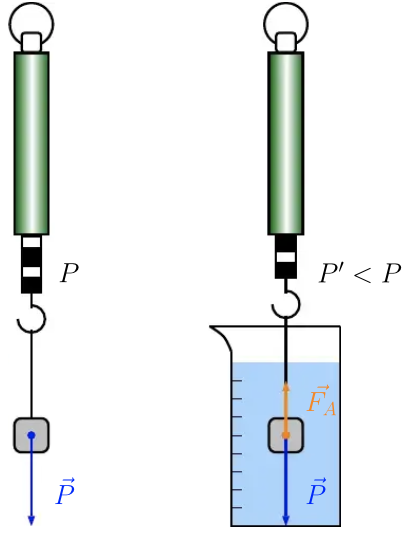
\includegraphics[scale=.4]{figures/archimede}
\end{minipage}


\section{Débit volumique}
\subsection{Régime permanent dans un tube}

\blocrouge{Définition}{Un régime permanent ou stationnaire signifie que les grandeurs physiques sont indépendantes du temps. Ici, la vitesse en un point M du fluide est constante au cours du temps.}

\etiquette{Signification} Le volume $V$ de fluide qui traverse une section pendant une durée $\Delta t$ correspond à un débit volumique $D$ $$D=\trou{\frac{V}{\Delta t}}$$

\etiquette{Exemples} 
\begin{itemize}
	\item Le débit sanguin circulant au travers de son coeur est de 5 L par minute. (à la maison convertir en mètre cube par seconde)
	\item Débit de la Seine: \SI{250}{\metre \cubed \per\second}
	\item Débit de l'eau au robinet \SI{e-3}{\metre \cubed \per\second}
\end{itemize}


\etiquette{Remarque} D'un point à un autre point du fluide la vitesse pourra changer. Voir exemple du tuyau pincé ci-après.

\subsection{Expression du débit volumique}
\begin{minipage}{.55\textwidth}
\begin{itemize}
	\item Où sont les particules de fluide qui vont traverser la section S entre les instants t=0 et t=$\Delta t$ ?
	\item La dernière particule de fluide à passer se situe à t=0 à une distance \trou{$l$ en amont de S} telle que $$l=\trou{v\times \Delta t}$$ 
	\item Le volume V s'écrit $\trou{l\times S}= \trou{v \times S \times \Delta t}$ 
\end{itemize}	
\end{minipage}
\hfill
\begin{minipage}{.40\textwidth}
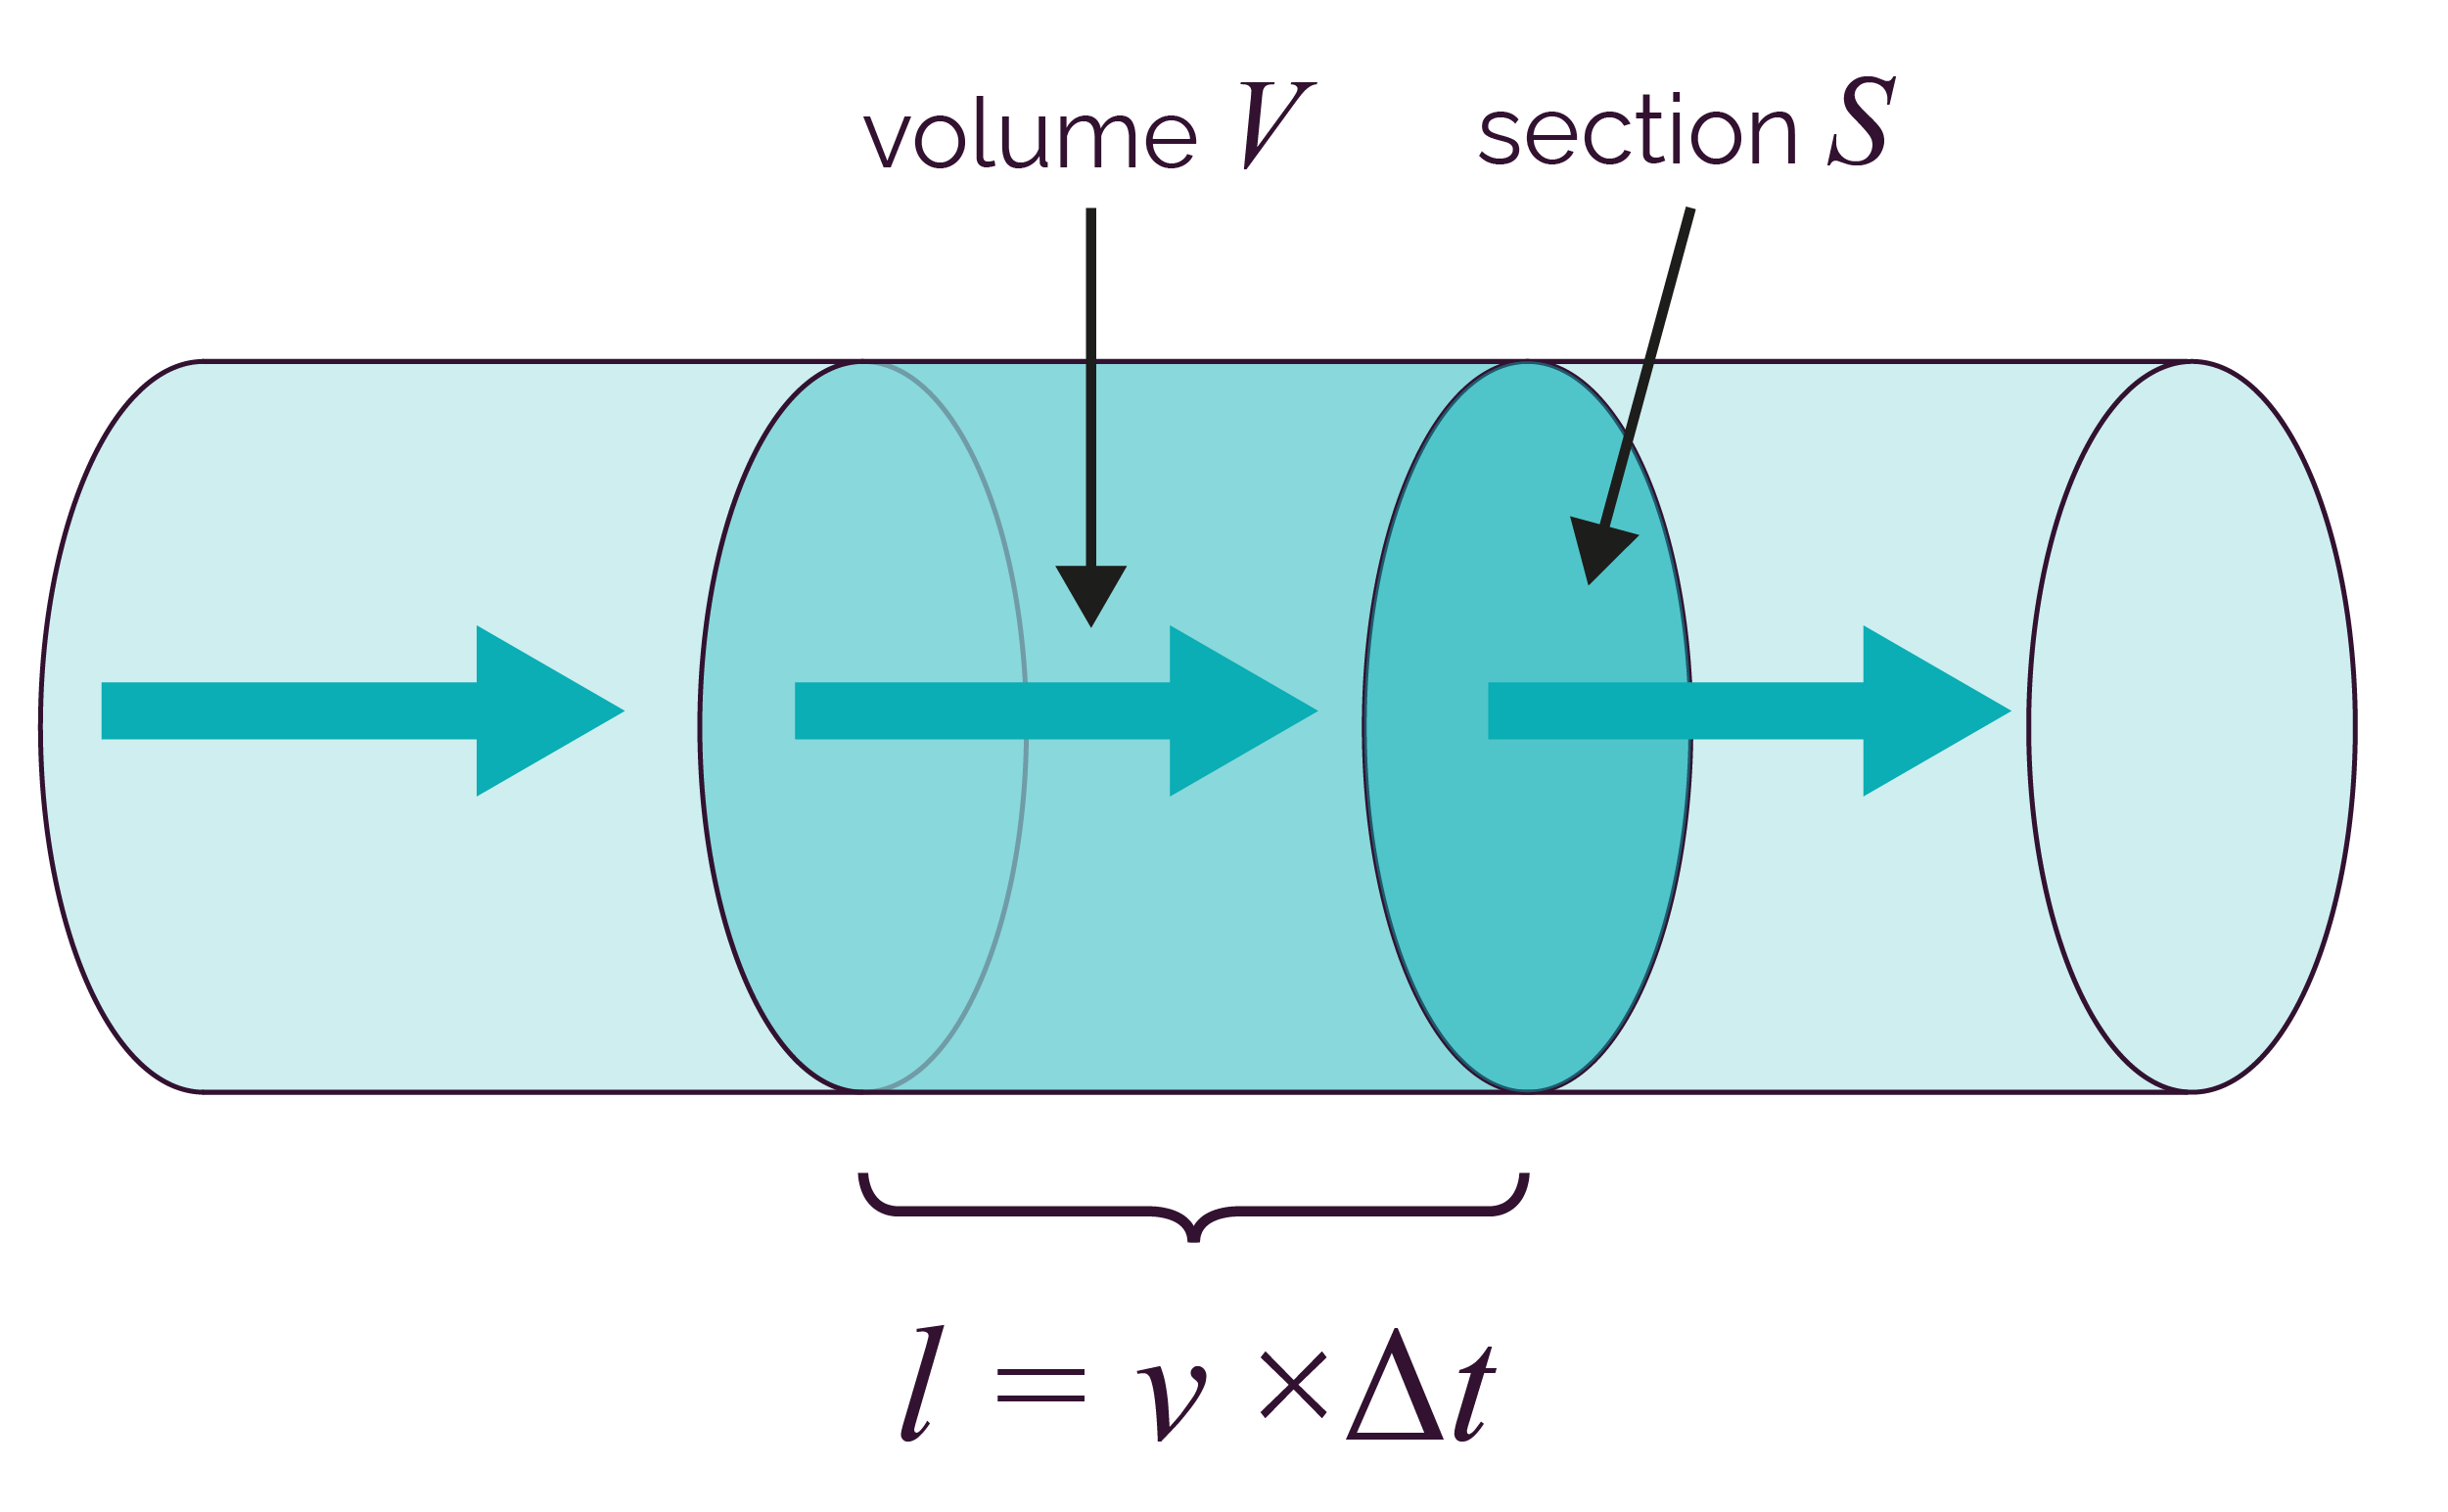
\includegraphics[scale=.3]{figures/debit_volumique}	
\end{minipage}


\blocrouge{A retenir}{Le débit volumique D est relié à la vitesse d'écoulement du fluide à travers une section S selon:$$D=\trou{S\times v}$$
D en \si{\metre \cubed \per \second } ; S en \si{\metre \squared} et $v$ en \si{\metre \per \second}}

\subsection{Conservation du débit}

\begin{minipage}{.50\textwidth}
En régime permanent le débit D se conserve.

 Observons le volume V de fluide qui traverse $S_1$ pendant $\Delta t$. Dans le même temps, le même volume traverse $S_2$.  
\end{minipage}
\hfill
\begin{minipage}{.45\textwidth}
\includegraphics[width=1\textwidth]{figures/consv_debit}
\end{minipage}

$$V=\trou{ S_1 \ell_1} = \trou{S_2 \ell_2}$$ 

\begin{align*}
	\ell_1 &= \trou{v_1} \times \Delta t\\
	\ell_2 &= \trou{v_2} \times \Delta t\\
\end{align*}

donc $$\boxed{D =\trou{S_1v_1} =\trou{S_2 v_2}=cste}$$

\blocgris{Application}{ Le débit d'un tuyau d'arrosage vaut \SI{e-4}{\meter \cubed\per \second}. Le rayon du tuyau vaut \SI{2}{\centi\metre}. 
\begin{enumerate}
	\item Calculer la vitesse de l'écoulement dans le tuyau.
	\item On pince le tuyau, son rayon devient \SI{0,5}{\centi\meter}. Que vaut la vitesse de l'eau à la sortie du tuyau ?
\end{enumerate}
}
\newpage

\subsection{Relation de Bernoulli}
\etiquette{Hypothèses}

\begin{minipage}{.50\textwidth}
  \begin{itemize}
	\item L'écoulement est \trou{permanent} (P, v et $\rho$ indépendant du temps).
	\item Le fluide est \trou{incompressible} ($\rho=cste$).
	\item A et B sont deux points situés sur \trou{une ligne de courant} (LDC).
	\item La relation de Bernoulli exprime la conservation de l'\trou{énergie mécanique} entre A et B.
\end{itemize}

\end{minipage}
\hfill
\begin{minipage}{.45\textwidth}
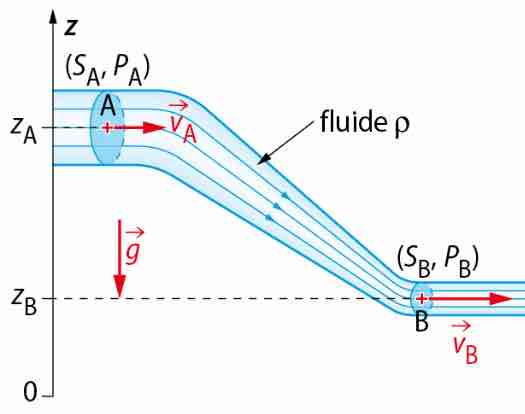
\includegraphics[width=.9\textwidth]{figures/Schema-Bernoulli}  

\end{minipage}

\blocrouge{Énoncé de la relation de Bernoulli}{On considère un fluide parfait, incompressible et en régime permanent.  A et B sont deux points appartenant à une même ligne de courant. On a $$\frac{1}{2}\rho\times  v_A^2 + \rho g z_A + P_A=\frac{1}{2}\rho\times  v_B^2 + \rho g z_B + P_B =cste$$}

\etiquette{Application: Effet Venturi}


Lorsque la variation d'altitude est négligeable. On constate que plus la vitesse du fluide est grande et plus sa pression est petite. Ce résultat s'appelle l'effet Venturi. 

Preuve de l'effet Venturi:

\begin{minipage}{.45\textwidth}
  On veut appliquer la relation de Bernoulli à l'écoulement ci-contre. On admet que  $S_1 >S_2$.
\end{minipage}
\hfill
\begin{minipage}{.55\textwidth}
\includegraphics{figures/venturi}
\end{minipage}
\begin{enumerate}
	\item Ecrire la conservation du débit volumique et en déduire que $v_2>v_1$.
	\item Choisir une ligne de courant avec les points A et B tels que $z_A=z_B$.
	\item Ecrire la relation de Bernoulli le long de la ligne  de courant. 
	\item En déduire que $P_1>P_2$.
\end{enumerate}
L'effet Venturi permet d'expliquer la portance d'une aile d'avion et aussi le fonctionnement d'une trompe à vide (voir exercices)

\begin{travail}
\begin{itemize}
	\item pages 288 à 295
	\item Poussée d'Archimède: 5 , 18 p 288 
	\item Conservation du débit volumique: 9
	\item Relation de Bernoulli: 2 , 17 , 21 , 25 , prepa ECE p 295
	\item Approfondir: 23 , 26
\end{itemize}
\end{travail}

% \setcounter{chapter}{15}
\chapter{Critère d'évolution et Piles}

\section{Une transformation est-elle toujours totale ?}
\subsection{Mise en évidence expérimentale}
Nous mettons de l'acide éthanoïque pur dans l'eau et nous obtenons une solution de $\SI{50}{\milli\liter}$ d'acide éthanoïque de concentration $\SI{1,0e-2}{\mole\per\liter}$. Le pH de cette solution est mesuré à 3,4.\\
\small	
\begin{tabular}{|l|p{1.5cm}|p{2cm}|p{1cm}|p{2cm}|p{2cm}|}
\hline 
  \multicolumn{2}{|c!{\protect\makebox[0cm]{:}}}{\textbf{Equation de la réaction}} &
 \multicolumn{1}{c!{\protect\makebox[0cm]{+}}}{%
      $\trou{\rm{CH_3COOH(aq)}}$} &
       \multicolumn{1}{c!{\protect\makebox[0cm]{ $\rightarrow$ }}}{%
      $\trou{\rm{H_2O(l)}}$} 
			&\multicolumn{1}{c!{\protect\makebox[0cm]{ + }}}
			{$\trou{\rm{CH_3COO^-(aq)}}$} 
			&\multicolumn{1}{c|}{
			$\trou{\rm{H_3O^+(aq)}}$} 
\tabularnewline


\hline 
Etat initial&
$x=0$&\trou{\num{5,0e-4}}
&\trou{excès}
&\trou{0}
&\trou{0}

\tabularnewline
\hline 
Etat intermédiaire&
$x$&\trou{\num{5,0e-4}-x}
&\trou{excès}
&\trou{x}
&\trou{x}

\tabularnewline
\hline 
Etat final&
$x=x_{f}$&$\rm \trou{\num{5,0e-4}-x_f}$
&\trou{excès}
&$\rm \trou{x_f}$
&$\rm \trou{x_f}$

\tabularnewline
\hline 
Etat final si tranformation&
$x=x_{max}$&$\trou{\num{5,0e-4}-x_{max}}$
&\trou{excès}
&$\rm \trou{x_{max}}$
&$\rm \trou{x_{max}}$
\tabularnewline
était totale & & & & & 
\tabularnewline
\hline
\end{tabular}\\
\normalsize
\\

Calcul de $\rm x_{max}$\\\trou{$\rm \num{5,0e-4}-x_{max}=0$ donc $\rm x_{max}=\SI{5,0e-4}{\mole}$}\\
Si la réaction était totale, quelle serait la valeur de $\rm x_f$ ?\\
$\rm \trou{x_f=\SI{5,0e-4}{\mole}}$\\
Quelle est la valeur expérimentale de $\rm x_f$ ?\\
\trou{$\rm x_f=[H_3O^+] \times V=10^{-3,4} \times 0,050=\SI{2,0e-5}{\mole}$\\
On remarque que $\rm x_f$ est différent de $\rm x_{max}$, ce qui signifie que la réaction n'est pas totale. Le réactif limitant ne disparaît pas totalement.}

\subsection{Qu'est ce qu'une transformation non totale ?}
\blocgris{Experience}{
Lorsqu'on ajoute à $\SI{50,0}{\milli\liter}$ de la solution d'acide éthanoique de concentration $\SI{1,0e-2}{\mole\per\liter}$ un peu d'ions $\rm CH_3COO^-$ en faisant en sorte que la variation de volume soit négligeable, on constate une augmentation du pH.
}

\etiquette{Interprétation} \\
\trou{On en déduit que $\rm[H_3O^+]$ diminue, ce qui signifie que les ions $\rm H_3O^+$ ont été consommés. Ils ont réagi avec les ions $\rm CH_3COO^-$ selon la réaction $\rm H_3O^++CH_3COO^-\longrightarrow H_2O+CH_3COOH$ }
\\
\trou{Il existe donc deux sens possibles pour la réaction : }
\begin{itemize}
\item \trou{ $\rm CH_3COOH$ réagit avec $\rm H_2O$ pour donner $\rm CH_3COO^-$ et $\rm H_3O^+$}
\item \trou{ $\rm CH_3COO^-$ réagit avec $\rm H_3O^+$ pour donner $\rm CH_3COOH$ et $\rm H_2O$}
\end{itemize}

\trou{La réaction est dite réversible.}
 \trou{
 $H_3O^+ + CH_3COO^- \leftrightharpoons +CH_3COOH$
 }
 \\

Le symbole $\leftrightharpoons$   signifie que la transformation est décrite par deux réactions  \trou{inverses.} On parle d'\textbf{équilibre chimique}.

\subsection{Equilibre dynamique d'un système}
Au niveau microscopique, le système chimique est le siège de deux réactions opposées. Les réactifs réagissent dans le sens \trou{direct} pour former les produits, et les produits réagissent dans le sens \trou{indirect} pour former les réactifs.\\
Au bout d'un moment, il se crée un \trou{équilibre}, et à l'échelle macroscopique, il \textbf{semble} qu'il ne se passe plus rien. 

L'état d'équilibre dynamique du système est alors atteint, et la vitesse de disparition de chaque espèce chimique est égale à sa vitesse d'apparition. Les quantités de matières sont stationnaires: l'équilibre chimique est atteint.
\subsection{Taux d'avancement final}
\blocrouge{Définition}{
Le taux d'avancement final $\tau$ (tau) d'une réaction est défini par le rapport :
\begin{center}
$\tau=\trou{\dfrac{x_f}{x_{max}}}$
\end{center}
}

\blocgris{Exemple}{
Calculer le taux d'avancement final pour la réaction entre l'acide éthanoïque et l'eau décrite au II.1
\\
\trou{$\tau=\dfrac{\SI{2,0e-5}{}}{\SI{5,0e-4}{}}=\SI{4,0e-2}{}$}
\\On constate que $\tau <  1$ ce qui traduit que la réaction n'est pas \texttt{totale}.}

\section{Evolution spontanée d'un système}
\subsection{Définition de l'activité}
L'activité d'une espèce chimique X se note $\alpha(X)$. C'est une grandeur sans dimension.\\
\begin{itemize}
\item Si X est une espèce en solution, alors $\alpha(X)=\dfrac{[X]}{c^0}$ avec $c^0=\SI{1}{\mole\per\liter}$
\item Si X est le solvant, alors $\alpha(X)=1$. Ce qui est très souvent le cas de l'eau.
\item Si X est une espèce solide, alors  $\alpha(X)=1$.
\end{itemize}

% suite

 \etiquette{Exemple}
 Exprimer l'activité de chaque espèce présente dans l'équation de la réaction de l'acide éthanoïque avec l'eau :\\
 \trou{$\alpha(CH_3COOH)=\dfrac{[CH_3COOH]}{c^0}$\\
 $\alpha(H_2O)=1$\\
$\alpha(CH_3COO^-)=\dfrac{[CH_3COO^-]}{c^0}$\\
$\alpha(H_3O^+)=\dfrac{[H_3O^+]}{c^0}$}

\subsection{Quotient de réaction}
\blocrouge{Définition}{
Considérons une réaction de la forme :$$aA + bB \leftrightharpoons cC +dD$$
 $Q_r$,  quotient de réaction est défini comme étant le produit :\\
 \begin{center}$Q_r=\trou{\dfrac{\alpha(C)^c\alpha(D)^d}{\alpha(A)^a\alpha(B)^b}}$\end{center}
 $Q_r$ est une grandeur sans unité.}

 \etiquette{Exemple} \\
 Exprimer le quotient de réaction dans le cas de la réaction de l'acide éthanoïque avec l'eau :\\
 \trou{$Q_r=\dfrac{\alpha(H_3O^+)\alpha(CH_3COO^-)}{\alpha(CH_3COOH)}=\dfrac{\dfrac{[H_3O^+]}{c^0}\dfrac{[CH_3COO^-]}{c^0}}{\dfrac{[CH_3COOH]}{c^0}}=\dfrac{[H_3O^+][CH_3COO^-]}{[CH_3COOH]c^0}$}


\subsection{Constante d'équilibre}
\blocrouge{Définition}{Lorsque le système chimique a atteint l'état d'équilibre, la valeur du quotient réactionnel est appelée: \trou{constante d'équilibre}. Elle se note K. $$\trou{Q_{r(eq)}= K}$$}
%\blocgris{Activité introductive}{
%On considère la réaction d'estérification, lors de laquelle un alcool réagit avec un acide pour donner un ester et de l'eau.\\
%La réaction étudiée fait réagir l'éthanol et l'acide éthanoïque. L'ester obtenu est l'éthanoate d'éthyle.\\
%L'équation de la réaction s'écrit : 
%$$CH_2CH_3OH + CH_3COOH\leftrightharpoons H_2O +CH_3COOCH_2CH_3$$
%
%\textbf{Cas \no1} : $n_i(alcool)=\SI{1,0}{\mole}$ ; $n_i(acide)=\SI{1,0}{\mole}$. \\ On obtient alors, à l'état final : $n_f(ester)=\SI{0,67}{\mole}$ ; $n_f(eau)=\SI{0,67}{\mole}$.\\
%\textbf{Cas \no2} : $n_i(alcool)=\SI{1,0}{\mole}$ ; $n_i(acide)=\SI{5,0}{\mole}$. \\ On obtient alors, à l'état final : $n_f(ester)=\SI{0,946}{\mole}$ ; $n_f(eau)=\SI{0,946}{\mole}$.\\
%\textbf{Cas \no3} : $n_i(alcool)=\SI{1,0}{\mole}$ ; $n_i(acide)=\SI{2,0}{\mole}$. \\ On obtient alors, à l'état final : $n_f(ester)=\SI{0,848}{\mole}$ ; $n_f(eau)=\SI{0,848}{\mole}$.\\
%Remarque : ici, l'eau n'est pas le solvant, on la prend donc en compte dans le calcul du quotient de réaction.\\
%Pour chaque cas, calculer le quotient de réaction à l'équilibre. Que remarquez-vous ?
%}

% suite

\etiquetterouge{Propriétés de K}
\begin{itemize}
	\item K ne dépend que de la \trou{température} mais pas de l'état initial du système.
	\item Pour la réaction d'un acide dans l'eau, K s'appelle la constante \trou{d'acidité} et se note Ka. 	
\end{itemize}



 \blocgris{Exemple}{
 Donner l'expression de la constante d'équilibre dans le cas de la réaction de l'acide éthanoïque avec l'eau (page 1) puis calculer sa valeur.\\ On rappelle que $[H_3O^+]_{eq}=\SI{3.98e-4}{\mol\per\liter}=[CH_3COO^-]_{eq}$ et  $[CH_3COOH]_{eq}=\SI{9.60e-3}{\mol\per\liter}$\\
 \trou{$K=\dfrac{\dfrac{[H_3O^+]_{eq}}{c^0}\dfrac{[CH_3COO^-]_{eq}}{c^0}}{\dfrac{[CH_3COOH]_{eq}}{c^0}}=\dfrac{[H_3O^+]_{eq}[CH_3COO^-]_{eq}}{[CH_3COOH]_{eq}c^0}$}\\
 \trou{$K=\dfrac{(10^{-3,4})^2}{\dfrac{\SI{5,0e-4}{}}{\SI{50e-3}{}}-10^{-3,4}}=\SI{1,65e-5}{}$}
 }
 \newpage
\subsection{Prévision du sens d'évolution}
%Reprenons l'exemple de la réaction d'estérification. 
%La réaction s'écrit : \\
%\begin{center}
%$$CH_2CH_3OH + CH_3COOH\leftrightharpoons H_2O +CH_3COOCH_2CH_3$$
%\end{center}
%L'acide est le réactif limitant. Au bout d'un certain temps, l'équilibre est atteint et le système n'évolue plus.\\
%Écrire le quotient de réaction à l'équilibre en notant $[ester]_{eq}$, $[acide]_{eq}$, $[alcool]_{eq}$ et $[eau]_{eq}$ les concentrations à l'équilibre.\\
%\begin{center}
%\trou{$Q_r=\dfrac{[ester]_{eq}[eau]_{eq}}{[acide]_{eq}[alcool]_{eq}}$}\\
%\end{center}
%Que pourrait-on faire pour que la réaction reparte dans le sens \no 1 ? \\
%\trou{On retire de l'eau. \\
%  Si [eau] diminue, on remarque que $Q_r$ diminue et la réaction évolue alors dans le sens 1.\\
%  On ajoute du réactif de l'alcool, réactif non limitant.\\
%  Si [alcool] augmente, on remarque que $Q_r$ diminue et la réaction évolue alors dans le sens 1.}
%  
  %
\etiquetterouge{Critères d'évolution}

On dispose d'un système chimique dont on connaît les concentrations initiales. On calcule le quotient réactionnel\textbf{ initial}: \trou{$Q_{ri}$}. On le compare à la constante d'équilibre K.
Il y a 3 cas à envisager: 

\begin{minipage}{0,58\linewidth}
\begin{enumerate}
\item Si $Q_r<K$, alors le système est hors équilibre et évolue dans le sens \trou{direct}.
\item Si $Q_r>K$, alors le système est hors équilibre et évolue dans le sens \trou{indirect}.
\item Si $Q_r=K$, alors le système a atteint son équilibre, et il \trou{n'évolue plus}.
\end{enumerate}
\end{minipage}
\begin{minipage}{0,40\linewidth}
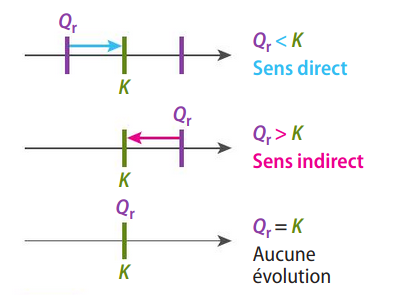
\includegraphics[scale=0.58]{figures/evolution/fig_K}
\end{minipage}

\etiquette{Exercice} 10 p 145 (important) 9 p 145



\newpage
\section{La pile, un transfert d'électrons}
\subsection{Un exemple de réaction d'oxydo-réduction}
\subsection*{Expérience}

\begin{figure}[h]
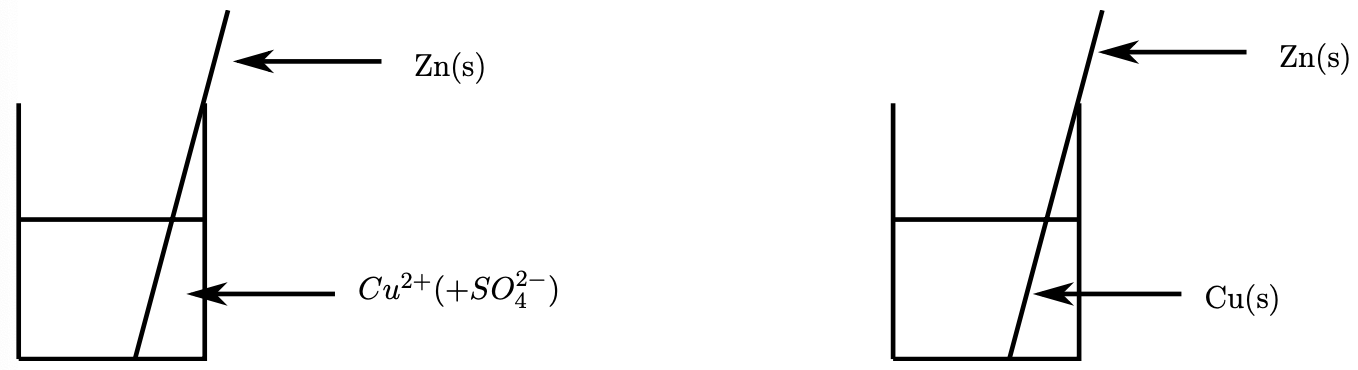
\includegraphics[scale=0.45]{figures/evolution/pile}
\end{figure}

\subsection*{Interprétation :}
On observe l'apparition de \trou{cuivre} sur la plaque de zinc. La réaction qui a eu lieu est donc :\\
\trou{$Cu^{2+}(aq) + 2e-=Cu(s)$}\\
D'où ces deux électrons peuvent-ils venir ?
Les deux électrons ont été cédés par \trou{le zinc : $Zn(s)=Zn^{2+}(aq) + 2e-$}\\
\trou{Donc, les deux électrons cédés par le zinc ont été captés par les ions $Cu^{2+}$}\\
On obtient donc l'équation de la réaction suivante :\\
\trou{$Zn(s)+Cu^{2+}(aq) \longrightarrow Zn^{2+}(aq) + Cu(s)$}


\etiquetterouge{Remarque} Cette réaction a eu lieu spontanément ce qui signifie qu'à l'état initial $Q_{ri}< K$. Vérifiez-le.

\subsection{Détournement d'électrons, réalisation d'une pile}
\etiquette{Montage expérimental} Pour réaliser une pile, on utilise de demi-pile. Un demi-pile est formée par l'association d'un métal et d'une solution contenant l'ion métallique.
\begin{center}
\begin{figure}[htp!]
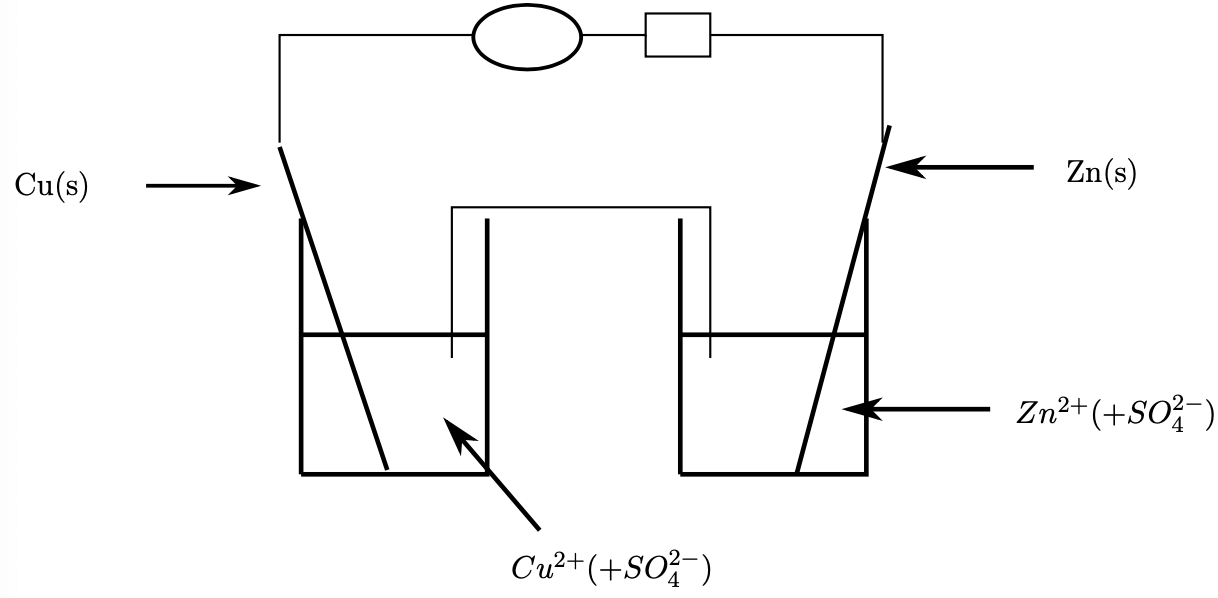
\includegraphics[scale=0.5]{figures/evolution/pile1}
\end{figure}
  \end{center}

\subsection*{Observations}

A l'aide d'un ampèremètre, on constate  \trou{qu'un courant circule de la lame de cuivre vers la lame de zinc à l'extérieur de la pile.}

\etiquette{Questions à se poser}

\begin{itemize}
	\item Où est le pôle positif ? le pôle négatif ?
	\item Quel est le sens de déplacement des électrons ? Celui du sens conventionnel du courant ? Les représenter sur le schéma de la pile.
	\item Les électrons se déplacent-ils dans les solutions ?
	\item Sachant que \textbf{l'oxydation} a \textbf{toujours} lieu à l\trou{'\textbf{anode}}. A quel pôle de la pile se situe l'anode ?
	\item Même travail pour la \textbf{cathode}.
\end{itemize}

\etiquetterouge{Fonctionnement de la pile}

Lorsque les électrons créés par la réaction d'\trou{oxydation} du zinc arrivent au niveau de la lame de cuivre, ils sont captés par les ions cuivre II pour former du cuivre. Les électrons sont forcés à circuler à l'\trou{extérieur} de la pile, ce qui génère un\trou{ courant électrique}, voilà pourquoi on peut évoquer un détournement d'électrons.

\subsection*{Équation globale de la pile} Lorsque la pile fonctionne (débite du \trou{courant}) cela se traduit par la réaction d'équation: 
$$Zn(s)+Cu^{2+}(aq) \longrightarrow \trou{Zn^{2+}(aq)+Cu(s)}$$

\subsection*{Rôle du pont salin}
Le pont salin assure la \trou{fermeture du circuit} électrique. Il est constitué d'un papier imbibé d'une solution contenant des ions (par exemple: $K^+ + NO_3^-$)\\
Il n'y a pas d'électron dans le pont salin puisque les électrons ne se trouvent jamais en solution. Ce sont les ions qui conduisent le courant en solution.

\etiquette{Travail}
Compléter sur le schéma le sens de déplacement des ions dans le pont salin.

\subsection*{Tension à vide ou f.e.m (force électromotrice)}
\begin{minipage}{0,6\linewidth}
La tension mesurée aux bornes de la pile lorsqu'elle ne débite pas est appelée \trou{tension à vide}. Elle est exprimée en volts.\\
Sur le schéma ci-contre, la borne V définit la borne positive de la pile
\end{minipage}
\begin{minipage}{0,4\linewidth}
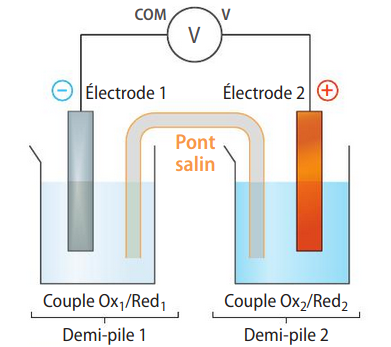
\includegraphics[scale=0.5]{figures/evolution/pile3}
\end{minipage}


\etiquetterouge{Important} Qu'est-ce qu'une pile usée ?\\
La pile en fonctionnement est un système hors \trou{ équilibre}, lorsqu'elle atteint \textbf{l'équilibre}, la réaction \trou{s'arrête}, le courant ne circule plus, la pile est \trou{\textbf{usée}}.

\subsection{Capacité d'une pile}
\blocrouge{Définition}{La capacité d'une pile, notée Q, est égale à la \trou{charge électrique} qui circule pendant la durée totale de son fonctionnement, de l'état initial à l'usure complète. La capacité de la pile s'exprime \trou{coulomb (C)}. \\ Rien à voir avec le quotient réactionnel Qr !!
}

Si l'on considère que l'intensité du courant I est constante pendant toute la durée de fonctionnement, alors on a :
$$\boxed{Q=\trou{I\times \Delta t}}$$
\begin{center}
 avec 
Q la capacité de la pile en coulombs(C)\\
I l'intensité du courant en ampères (A)\\
$\Delta t$ le durée de vie de la pile en secondes (s)
\end{center}
On peut également calculer la capacité d'une pile grâce à l'expression :$$\boxed{Q=\trou{n(e^-) \times F}}$$
\begin{itemize}
	\item $n(e^-)$ le nombre d'électrons échangés pendant le fonctionnement.
	\item F la constante de faraday : $F=e\times N_a=\SI{9,65e4}{\coulomb\per\mole}$ C'est la charge d'une mole d'électrons.

\end{itemize}
%\newpage
\etiquette{Exercices sur les piles}
\begin{itemize}
	\item 14 
	\item  16
	\item  19
	\item  28 p 146
\end{itemize}

Type bac: \url{https://www.labolycee.org/defibrillateur-cardiaque-implantable}
%
%
%\section{Electrolyse}
%\subsection{Transformation forcée}
%\etiquetterouge{Idée forte} En apportant de l'énergie électrique à un système chimique, il est possible de\trou{ renverser }le sens de l'évolution spontané d'une réaction chimique, c'est \textbf{\trou{l'électrolyse}}. L'énergie est apporté par un \textbf{générateur} qui va \textbf{\trou{imposer le sens }du courant} et donc celui des échanges d'électrons.
%
%\subsection{Electrolyse d'une solution de chlorure d'étain}
%\etiquette{Montage}
%
%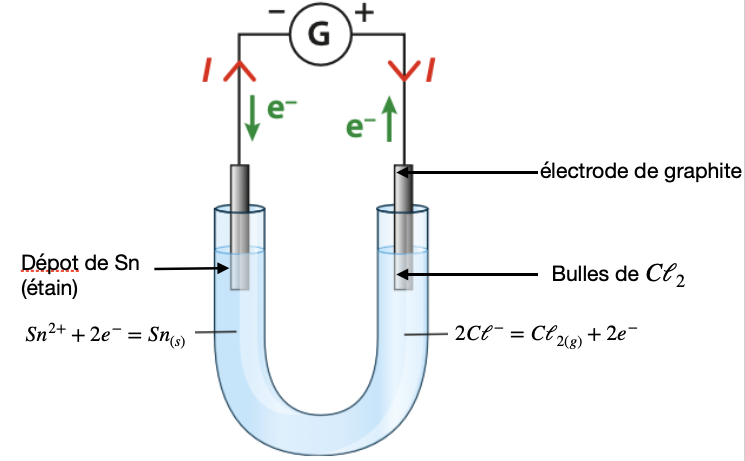
\includegraphics[width=12 cm]{figures/electrolyse_3}
%
%Vidéo de l'expérience: \url{https://www.youtube.com/watch?v=0KI65y_b5y4}
%
%\subsection{Obtention des équations redox}
%
%On sait que :
%\begin{itemize}
%	\item Le courant I et le sens des $e^-$ est imposé par le générateur. 
%	\item Initialement les seules espèces chimiques présentes sont: $C\ell^-$ et $Sn^{2+}$.
%	\item Les couples sont $C\ell_{2(g)} / C\ell^-$ et $Sn^{2+} / Sn$.
%	\item Equations redox des couples $$\trou{C\ell_{2(g)}} + 2e^- = \trou{C\ell^-}$$ $$Sn^{2+}+\trou{2e^-}=\trou{Sn}$$
%\end{itemize}
% On en déduit que: 
%\begin{itemize}
%	\item Les électrons arrivent à gauche. Il sont consommés selon $$\trou{Sn^{2+}}+2e^- = \trou{Sn}$$
%	\item Les électrons qui partent de l'électrode à droite sont produits par $$2C\ell^-=C\ell_{2(g)}+\trou{2e^-}$$
%\end{itemize}
%
%\subsection{Interprétation chimique}
%
%Durant l'électrolyse, on observe la réaction d'équation $$\trou{2C\ell^-+Sn^{2+}}\longrightarrow \trou{C\ell_{2(g)}+Sn_{(s)}}$$ 
%
%\blocgris{Questions}{
%On donne:  l'activité initiale du dichlore vaut 1, $[Sn^{2+}]_i = 0,5$ mol/L et $[C\ell^-]_i = 1$ mol/L.
%\begin{enumerate}
%	\item Quelle est la valeur de $Q_{ri}$ ? 
%	\item Sachant que K = \num{e-51}. Quelle est le sens spontanée de la réaction chimique.
%	\item Justifier qu'il s'agit ici d'une réaction forcée.
%\end{enumerate}
%}
%\section{Quelques couples oxydant-réducteur usuels}
%\blocgris{Demi-équations}{
%Pour chacun des couples ci-dessous, écrire la demi-équation d'oxydo-réduction : 
%\begin{itemize}
%\item L'eau de javel est une solution d'ion hypochlorite $ClO^-$ oxydant du couple : $ClO^-/Cl^-$\\
%\trou{$ClO^-+H_20+2e-=Cl^-+2HO^-$}
%\item le dioxygène $O_2$ est l'oxydant du couple $O_2/H_2O$\\
%\trou{$O_2+4e-+4H^+=2H_2O$}
%\item le dichlore $Cl_2$ est l'oxydant du couple $Cl_2/Cl^-$\\
%\trou{$Cl_2+2e-=2Cl^-$}
%\item l'acide ascorbique ou vitamine C est le réducteur du couple $C_6H_6O_6/C_6H_8O_6$\\
%\trou{$C_6H_6O_6 +2H^+  = C_6H_8O_6$}
%\item le dihydrogène $H_2$ est le réducteur du couple $H^+/H_2$.\\
%\trou{$2H^+ +2e-=H_2$}
%\end{itemize}
%}
%\etiquette{Remarque}
%Les éléments des deux premières colonnes du tableau périodique sont les éléments du bloc s. Ils ont tous un ou deux électrons sur leur couche externe. Ils sont donc susceptibles de les perdre, ce qui fait d'eau des \trou{réducteurs}
%
%\etiquette{Récap du cours sur électrolyse} \url{https://www.youtube.com/watch?v=w3lg9HDBMKw}
%
%
%\etiquette{Exercices sur l'électrolyse}
%1, 2, 8, 12 et 18 p 184
%type bac: \url{https://www.labolycee.org/corrosion-et-protection-des-metaux}

 \setcounter{chapter}{16}
\chapter{Thermodynamique (partie 1)}
\section{Le modèle du gaz parfait}
\subsection{Description}

Le modèle du gaz parfait est un ensemble d'hypothèses qui forme une description microscopique d'un gaz. Ces hypothèses sont liées à des propriétés microscopiques et à des grandeurs macroscopiques mesurables: P, V et T.

\begin{table}[hbt]
  \begin{tabular}{|p{10cm}|p{7cm}|}
  \hline
A l'échelle microscopique    & A l'échelle macroscopique \\
    \hline \hline
Les particules (atomes ou molécules) de gaz sont en mouvement \trou{désordonné}. Ces particules sont considérées comme des points matériels (masse mais taille nulle). Il n'y a \trou{aucune interaction} entre les particules     & La température T en K du gaz est reliée aux \trou{vitesses moyennes} des particules qu'il contient \\
\hline
Nombreux chocs entre les particules et la paroi du récipient    & L'ensemble de \trou{ces chocs} engendre une pression P sur la paroi.  \\
\hline
Les particules sont \trou{très espacées} les unes des autres & La masse volumique $\rho=\frac{m}{V}$ est très faible environ 1 kg par mètre cube \\
\hline
  \end{tabular}

\end{table}

\blocrouge{Equation d'un gaz parfait}{

Les grandeurs qui caractérisent l'état d'un gaz parfait vérifient l'équation:
$$P\times V = \trou{n\times R\times T}$$
P: pression en Pa ; V: volume du gaz en $m^3$ ; $n$ quantité de matière de gaz en mol ; T température en K \\
R est la constante des gaz parfaits et vaut 8,31 J/K\\
T (en K) = 273 + température en \SI{}{ \celsius}

}


\subsection{Limites du modèle}

Le modèle du gaz parfait est bien vérifié si :
\begin{itemize}
	\item La pression du gaz n'est pas trop grande
	\item les interactions entre particules sont négligeables
	\item la taille des particules est négligeable
\end{itemize}

\section{Premier Principe de la Thermodynamique}
\etiquetterouge{A retenir} Les énergies se présentent sous différentes formes ou manière de s'échanger mais toutes se comptent en \trou{joule  } de symbole J. C'est l'unité légale de mesure de l'énergie.

\subsection{Énergie interne d'un système }
Tout système macroscopique est composé d'un grand nombre d'entités\footnote{entité microscopique = atome, ion ou molécules} microscopiques en mouvement et en interaction entre elles. Chacune possède une \textbf{\trou{énergie cinétique microscopique}}, liée à l'agitation thermique et une \textbf{énergie \trou{potentielle } microscopique} liée à ses interactions avec les autres.\\
\blocrouge{Définition}{
L'énergie interne U d'un système macroscopique est égale à la somme des énergies \trou{ microscopiques } (cinétique et potentielle) de toutes les entités microscopiques qui constituent le système. Elle s'exprime en \trou{joule} de symbole \trou{J}.
}

En pratique, on ne s'intéresse pas à la valeur de l'énergie interne, on s'intéresse à sa variation: $\Delta U = U_f - U_i$ cf premier principe.

\etiquetterouge{Important}L'énergie interne U augmente quand \trou{la température du système augmente.}

\subsection{Énergie totale}

L'énergie totale d'un système est:\\
\trou{la somme des énergies potentielle de pesanteur, cinétique (macroscopique) et de l'énergie interne.\\
On note $E_{tot}=E_{pp}+E_c+U$}

\subsection{Travail échangé: W}
Le système peut échanger de l'énergie sous forme de travail noté W. Cette situation s'observe lorsque le système subit au moins une force qui travaille. 

\etiquette{Exemples:}
\begin{itemize}
	\item Système: gaz contenu dans un piston. On pousse le piston de manière à comprimer le gaz. Les forces de pression travaillent.
	\item Vous frottez vigoureusement vos mains entre elles, les forces de frottements travaillent et cette énergie reçue augmente l'énergie interne de vos mains et ainsi leurs températures.
	\item On considère un récipient rempli d'eau dans lequel est plongé une hélice reliée à un moteur.\\
On mesure la température de l'eau après avoir fait tourner l'hélice. On constate une augmentation de la température. On en déduit que l'énergie interne de l'eau a  \trou{augmenté} suite à un transfert d'énergie par travail.(L'hélice se déplace). Voir expérience de Joules pour plus d'informations.

\end{itemize}

\subsection{Transfert thermique: Q}

Ce transfert se fait sans aucun mouvement de la part du système. Il est en général dû à une différence de température entre le système et le milieu extérieur.Le transfert thermique se fait d'un corps chaud vers un corps froid. 
\begin{center}
	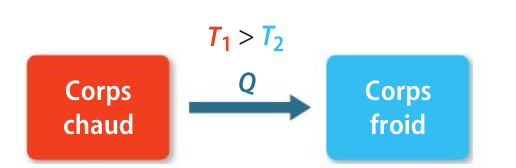
\includegraphics[scale=0.5]{figures/thermo/fig_sens}	
\end{center}


\blocrouge{Convention}{
Le travail W et le transfert thermique Q sont comptés 
\begin{itemize}
	\item positivement si l'énergie est reçue par le système
	\item négativement si l'énergie est cédée par le système au milieu extérieur
\end{itemize}

}

\blocgris{Application}{ Un bloc d'acier à 50$^{\circ}$C est plongé dans 25 cL d'eau à 15$^{\circ}$C. Le système étudié est le bloc d'acier.
\begin{enumerate}
	\item Faire un schéma. Représenter par une flèche le transfert thermique: Q entre le bloc d'acier et l'eau.
	\item Dans cette situation, quel est le milieu extérieur ?
	\item En admettant le bloc d'acier cède 10 J par transfert thermique à l'eau. Que vaut le transfert thermique Q échangé avec le milieu extérieur ?
	\item En considérant l'eau comme système, quel est le transfert thermique Q' échangé avec l'extérieur dans la même situation. 
\end{enumerate}
}



\subsection{Énoncé du premier principe}

\blocrouge{Premier principe de la thermodynamique\footnote{Par définition un principe ne se démontre pas contrairement à un théorème. On admet donc que ce principe est vrai et on en tire des propriétés, des conséquences, des applications...}}{
La variation d'énergie interne pour un système immobile à l'échelle macroscopique est égale à la somme des énergies échangées par le système avec l'extérieur, sous forme de travail W et de transfert thermique Q.\\
On a donc :$$ \trou{\Delta U=W+Q}$$
}
\etiquette{Méthode Générale} Le premier principe permet de faire un bilan d'énergie. Dans un exercice on fera attention à bien:
\begin{itemize}
	\item Définir le système étudié et son milieu extérieur avec lequel il échange de l'énergie.
	\item Identifier et catégoriser tous les transferts d'énergie. Est-ce un travail W ou un transfert thermique Q ?
	\item Le travail est-il reçu (W>0) ou fourni (W<0) ? idem pour Q
	\item Calculer la somme des transferts : W + Q 
	\item Confronter la somme des transferts à la variation d'énergie interne $\Delta U$
\end{itemize}


\subsection{Cas important d'un système incompressible}

Les liquides et les solides sont des systèmes que l'on peut considérer incompressibles. Dans ce cas, le travail $W$ des forces de pression est \trou{nul }.  Ces systèmes n'échangent que du transfert \trou{thermique Q } avec l'extérieur.

\etiquette{Exemples}
Observez les 4 transferts thermiques suivants.
Identifier les grandeurs qui influent sur la variation de température d'un système qui reçoit un transfert thermique Q.
\begin{center}
	\includegraphics[scale=.9]{figures/thermo/capacite_thermique}
\end{center}



\blocrouge{Relation Q et $\Delta T$}{
Lorsqu'un système (incompressible)   échange avec l'extérieur un transfert thermique Q sa température varie de $\Delta T$  selon $$Q = C\times \Delta T= C\times(T_f-T_i)$$
C est appelée la capacité thermique du système


Unités: Q en J ; C en J/K ; $\Delta T$ en K
}

\etiquette{Remarque} Lors de cette transformation, l'énergie interne varie. D'après le premier principe on a $\Delta U = Q$ car $W=0$ (incompressible).


\etiquetterouge{Sens Physique !} Il faut penser la capacité thermique du système comme l'énergie qu'il doit recevoir pour augmenter sa température de $1^{\circ}$C.

\etiquette{Culture}

La capacité thermique d'un litre d'eau est 4180 J/K. Cela signifie qu'en transférant une énergie Q= 4180 J à un litre d'eau, on augmente de \SI{1}{\celsius} sa température (peu importe sa température initiale tant qu'il n'y a pas changement d'état).

\etiquette{Capacité thermique massique} 

Dans les exercices, on trouvera souvent la capacité thermique massique $c$ et non la capacité thermique du système de masse $m$. Naturellement pour un matériau donné, plus le système est gros (plus sa masse est importante) plus il faut d'énergie pour augmenter sa température de $1^{\circ}$C. 
$$C = m\times c$$
C capacité thermique du système en J/K ; m: masse du système en kg et $c$: capacité thermique massique en J/kg/K

\blocrouge{Astuce}{Regardez les unités, si $c$ est par unité de masse, multipliez le par la masse du système}

\blocgris{Application}{On place 500 mL d'eau froide à $15^{\circ}$C dans un casserole. Pour préparer du thé, on chauffe cette eau jusqu'à $85^{\circ}$C. Pour cela, on utilise une plaque chauffante de 800 W.\\ Données: capacités thermiques massiques: $c_{eau}=4,18\:kJ.kg^{-1}.K^{-1}$ ; $c_{fer}=444\:J.kg^{-1}.K^{-1}$
\begin{enumerate}
	\item Calculer le transfert thermique Q reçu par l'eau pendant le chauffage.
	\item En admettant que toute l'énergie de la plaque chauffante est transférée à l'eau, combien de temps faut-il au système pour atteindre $85^{\circ}$C ?
	\item On recommence la même expérience (même durée de chauffage que la question précédente) en remplaçant les 500 mL d'eau par 500 g de fer. Quelle est la température atteinte par le bloc de fer ?
	\item Conclure
\end{enumerate}

}
\newpage

\blocgris{Synthèse}{A l'aide des questions suivantes réalise une synthèse 
\begin{enumerate}
	\item Quelles sont les grandeurs macroscopiques qui permettent de décrire un gaz ?
	\item Quelles sont les hypothèses du modèle du gaz parfait ? Quelles sont les limites de ce modèle ?
	\item Comment s'écrit l'équation d'un gaz parfait. Pourquoi dit-on que c'est une équation d'état ? Précise toutes unités de cette équation.
	\item Quelles différences entre énergie interne et énergie mécanique ?
	\item Quelles sont les deux manières pour un système de modifier son énergie interne ?
	\item Comment évolue la température lorsque l'énergie interne augmente ?
	\item Dans le cas d'un système incompressible qui reçoit Q quel relation y a-t-il entre Q et $\Delta$ U ?
	\item Explique simplement ce qu'est la capacité thermique d'un système ?
	\item Donne la relation entre la capacité thermique massique $c$, la masse, $\Delta T$ et Q pour un système incompressible.
\end{enumerate}
}

\etiquetterouge{Exercices à faire}
\begin{itemize}
	\item 18 ; 22 p 314
	\item 27 ; 28 p 316
	\item Questions 1,2,3 et 4 du sujet: \url{https://prod.labolycee.org/bac-2023-centres-etrangers-1-jour-1}
\end{itemize}

 \section{Transfert thermique et Flux}
\subsection{Les 3 Modes de transferts thermiques}

Il y a 3 manières pour un système pour recevoir du transfert thermique\footnote{on pourrait dire pour recevoir de la chaleur mais ce mot est banni pour cause de confusion avec la température}


\begin{itemize}
\item le transfert thermique \textbf{par rayonnement} : \trou{ transfert d'énergie sous forme d'ondes électromagnétiques, principalement dans l'infrarouge, émis par des objets en raison de leur température.}
\item le transfert thermique \textbf{par \trou{convection}} : l'énergie thermique se transmet de proche en proche dans un fluide avec \textbf{mouvement d'ensemble} de celui-ci.
\item le transfert thermique \textbf{par \trou{conduction}} : Il y a contact entre le système et l'extérieur. L'agitation thermique se transmet de proche en proche dans la matière \trou{sans déplacement} d'ensemble de celle-ci.\\
\begin{center}
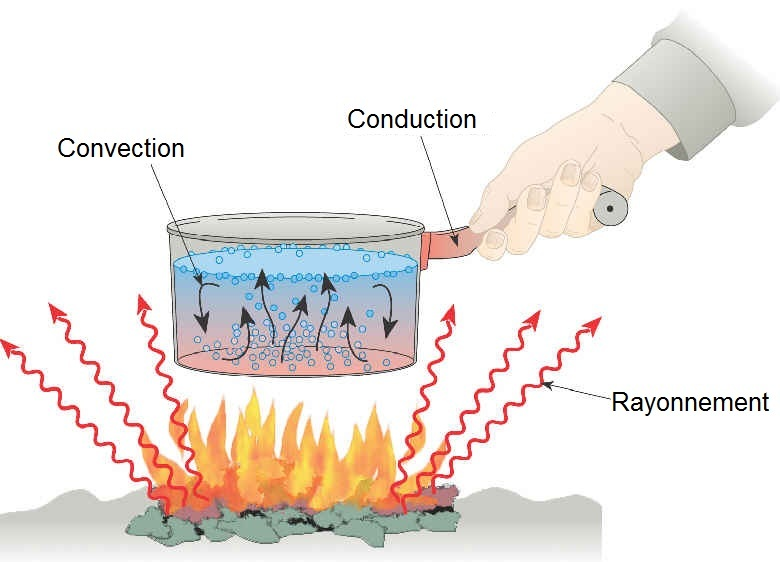
\includegraphics[scale=0.5]{figures/thermo/convection}
\end{center}
\end{itemize}

%\newpage
%\blocgris{Application}{Repérer dans le texte suivant les différents transferts thermiques et essayez de regrouper ces exemples en trois catégories : \\
%\textit{C'est le printemps, vous vous prélassez au soleil. Il fait chaud.\\
%Vous rentrez ensuite préparer votre repas. Au menu, spaghettis bolognaise. Vous placez votre casserole d'eau sur la plaque électrique. L'eau se réchauffe et commence à bouillir. Vous y plongez vos pâtes. Vous mettez la sauce bolognaise à réchauffer dans une autre casserole et vous oubliez votre cuillère en inox dedans. Au moment de remuer, impossible de toucher la cuillère, elle est bien trop chaude. Vous allez donc chercher une cuillère en bois.\\
%Une fois repus, vous vous préparez une boisson chaude. Vous mettez votre tasse au micro-onde. En trente secondes, c'est chaud. Vous entourez votre tasse de vos mains pour les réchauffer puis vous vous asseyez, le dos contre le radiateur chaud. \\
%Au moment où vous montez vous coucher, vous vous rendez compte qu'il fait bien plus chaud à l'étage qu'au rez de chaussée alors que les radiateurs ne sont allumés qu'en bas.\\
%Vous vous endormez jusqu'au petit matin où vous débuterez une nouvelle journée rythmée par les transferts thermiques.}
%}
%\newpage
\subsection{Le flux thermique}
\etiquette{Contexte} On considère une paroi qui sépare deux milieux de températures différentes $T_1$ et $T_2$ telle que $T_1>T_2$. L'écart de température provoque de la \trou{conduction} entre la face chaude et la face froide. On dit qu'un flux\footnote{flux vient du latin fluxus qui signifie écoulement} thermique noté $\Phi$ traverse la paroi. Ce flux est une \trou{puissance} elle s'exprime donc en Watt de symbole \trou{W}.


\begin{center}
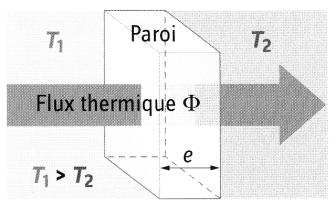
\includegraphics[scale=0.5]{figures/thermo/fig1}
\end{center}


\etiquette{Interprétation Physique} $\Phi$ représente l'énergie qui traverse la paroi chaque seconde. $$\boxed{1\:W = 1 \:J/s}$$

\subsection{Résistance thermique}
\begin{itemize}
	\item Plus l'écart de température est grand et plus la conduction est \trou{importante}, plus $\Phi$ est \trou{grand}.
	\item Le flux dépend du matériau qui constitue la paroi et des dimensions de la paroi. On parle alors de la \trou{résistance thermique de la paroi}, elle se note $R_{th}$.
\end{itemize}

\blocrouge{Formules}{$$\Phi=\frac{T_1 - T_2}{\trou{R_{th}}}$$ Unités: $\Phi$ en W (ou J/s) ; $T_1$, $T_2$ en K ; $R_{th}$ en K/W $$R_{th}=\frac{\trou{ e }}{\lambda . S}$$ Unités: e: en m ; $S$ en $m^2$ et $\lambda$: conductivité thermique de la paroi en $\SI{}{\watt\per\kelvin\per\meter}$
}

\etiquette{Conséquences}
\begin{itemize}
	\item Le flux est d'autant plus grand que la résistance thermique $\rm R_{th}$ est \trou{petite}.
	\item Ce flux est d'autant plus grand que la différence de température $\rm T_1-T_2$ est \trou{grande}
	\item Plus l'épaisseur de la paroi est grande, plus sa résistance thermique est \trou{grande} et plus elle est isolante/conductrice.
	\item Plus la surface de la paroi est grande, plus sa résistance thermique est \trou{petite.}
\end{itemize}



\blocgris{Exercice}{On considère un mur en béton de surface 10 $m^2$ et d'épaisseur 15 cm. Ce mur sépare l'intérieur d'une habitation dont la température est \SI{20}{\celsius} et l'extérieur dont la température est $5^\circ$C. La conductivité thermique du béton est $\SI{0,013}{\watt\per\kelvin\per\meter}$.
\begin{enumerate}
	\item Calculer la résistance thermique du mur.
	\item En déduire le flux thermique traversant le mur.
\end{enumerate}
%\vspace{7  cm}
}

\begin{travail}
\begin{itemize}
	\item Résistance thermique: \url{https://labolycee.org/isolation-thermique-du-rover-perseverance}
	\item Application du premier principe: \url{https://labolycee.org/linteret-energetique-dune-pac}
	\item Autre sujet de bac: \url{https://labolycee.org/le-sauna}
\end{itemize}

\end{travail}


\section{Température terrestre moyenne}

\subsection{Corps Noir et Rayonnement Thermique}

Le rayonnement thermique du Soleil et de la Terre sont très bien décrits par le modèle du \textbf{corps noir}. Ce modèle décrit la production de rayonnement thermique sous l'effet de la température.

\etiquette{Loi de Stefan-Boltzmann} La puissance rayonnée par unité de surface par un corps noir vaut :
$$\boxed{P=\sigma\ T^4}$$

où $\sigma = \SI{5,67e-8}{W.m^{-2}.K^{-4}}$ est la \textbf{constante de Stefan-Boltzmann}.

\subsection{Hypothèses du modèle simplifié}

\begin{itemize}
	\item La Terre est à \textbf{l'équilibre thermique} : l'énergie reçue = l'énergie émise
	\item La Terre se comporte comme un \textbf{corps noir de température $T$}
	\item Le système Terre-Atmosphère reçoit une puissance solaire moyenne par unité de surface : $$P_S= \SI{340}{W.m^{-2}}$$
	\item Une fraction $A$ de cette puissance est \textbf{réfléchie} (albédo terrestre) : $$A=0,34$$
	\item La puissance surfacique \textbf{absorbée} par la Terre vaut donc : $$P_{absorbee}= (1-A)\times P_S$$
	\item \textbf{L'atmosphère} absorbe une fraction $a=0,45$ du rayonnement infrarouge émis par la surface terrestre et le \textbf{renvoie partiellement vers la surface} (effet de serre)
\end{itemize}

\subsection{Schéma du bilan énergétique}
\begin{center}
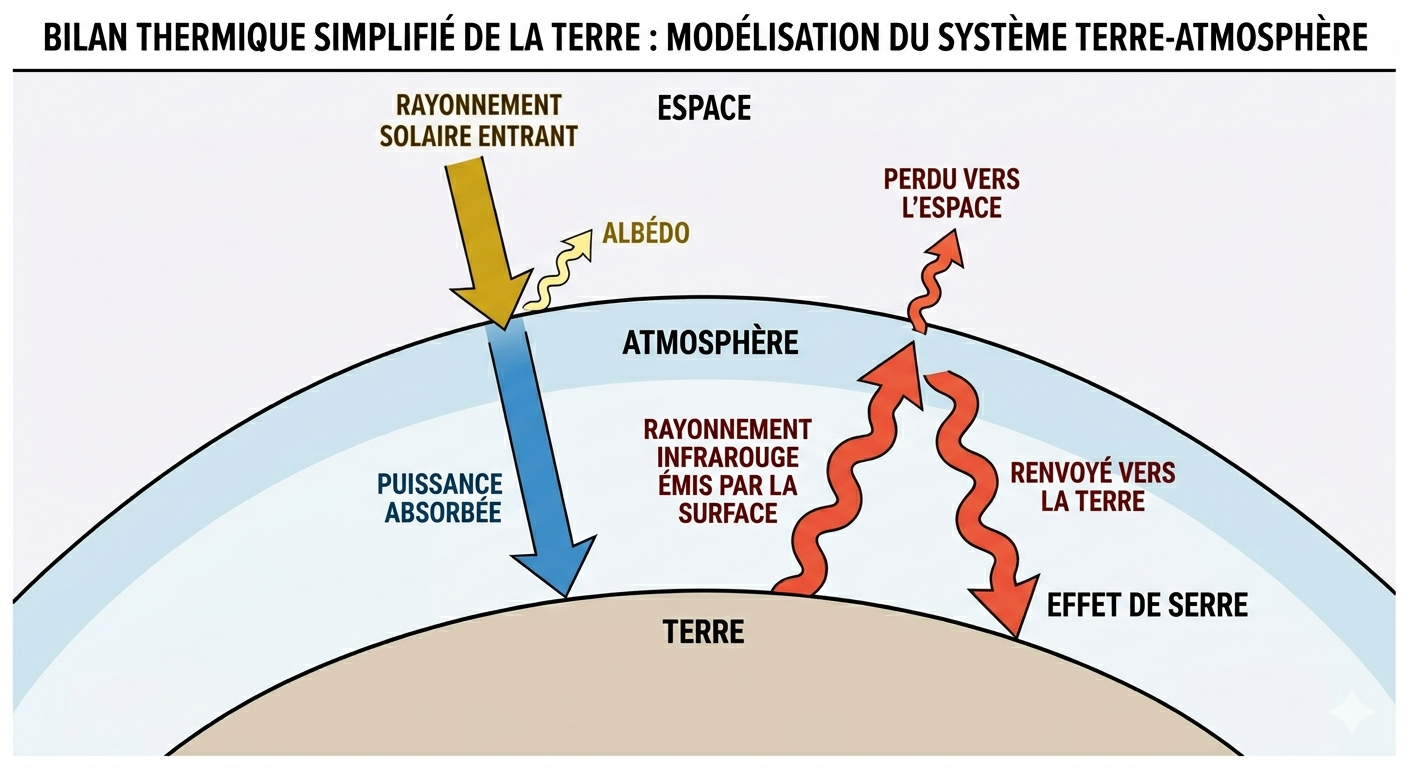
\includegraphics[width=.7\textwidth]{figures/thermo/albedo.png}
\end{center}
\subsection{Bilan énergétique sans atmosphère}

En l'absence d'atmosphère, la Terre ne reçoit que le rayonnement solaire et émet uniquement vers l'espace.

\etiquette{Équilibre thermique} À l'équilibre :
$$P_{absorbee} = P_{emise}$$

$$(1-A) \times P_S = \sigma T_0^4$$

\etiquette{Calcul} En isolant la température :
$$T_0 = \left[\frac{(1-A) \times P_S}{\sigma}\right]^{1/4}$$

$$T_0 = \left[\frac{0,66 \times 340}{5,67 \times 10^{-8}}\right]^{1/4} = \left[\frac{224}{5,67 \times 10^{-8}}\right]^{1/4}$$

$$\boxed{T_0 \approx \SI{255}{K} = \SI{-18}{\celsius}}$$

\etiquette{Interprétation} Sans atmosphère, la Terre serait gelée à $-18°C$ !

\subsection{Bilan énergétique avec atmosphère : l'effet de serre}

L'atmosphère absorbe une fraction $a = 0,45$ du rayonnement infrarouge émis par la Terre et le \textbf{renvoie partiellement vers la surface}. Cela génère un surplus d'énergie à la surface.

\etiquette{Nouveau bilan} À l'équilibre (incluant le retour de l'IR par l'atmosphère) :
$$(1-A) \times P_S + \text{(rayonnement renvoyé par l'atmosphère)} = \sigma T^4$$

Le rayonnement renvoyé par l'atmosphère crée un \textbf{effet de serre} qui augmente la température.

\etiquette{Résultat qualitatif} L'inclusion de cet effet de serre augmente considérablement la température terrestre :

$$\boxed{T \approx \SI{288}{K} = \SI{15}{\celsius}}$$

Cette température correspond à la \textbf{température réelle moyenne de la Terre} !

\etiquette{Différence observée}
$$\Delta T = T - T_0 = 288 - 255 = \SI{33}{K}$$

Cette différence de \textbf{33 K} est directement due à l'\textbf{effet de serre atmosphérique}.

\subsection{Influence de l'albédo et de l'effet de serre sur la température}

\etiquette{Dépendance à l'albédo} La température dépend de l'albédo selon :
$$T \propto (1-A)^{1/4}$$

\begin{itemize}
	\item Si l'albédo $A$ \textbf{augmente} (plus de nuages, plus de glace) $\Rightarrow$ moins d'énergie absorbée $\Rightarrow$ \trou{température diminue}
	\item Si l'albédo $A$ \textbf{diminue} (fonte des glaces) $\Rightarrow$ plus d'énergie absorbée $\Rightarrow$ \trou{température augmente}
\end{itemize}

\etiquette{Dépendance à l'effet de serre}

Si la concentration en \textbf{CO$_2$ augmente} $\Rightarrow$ l'atmosphère absorbe davantage l'infrarouge terrestre $\Rightarrow$ \trou{température augmente}
%
%\blocgris{Boucles de rétroaction}{
%\begin{itemize}
%	\item \textbf{Rétroaction positive} : Fonte de glace $\downarrow A$ $\Rightarrow$ absorb. $\uparrow$ $\Rightarrow$ chauffage $\uparrow$ $\Rightarrow$ fonte $\uparrow$ (amplifie)
%	\item \textbf{Rétroaction négative} : Aérosols volcaniques $\uparrow A$ $\Rightarrow$ absorb. $\downarrow$ $\Rightarrow$ refroidissement $\downarrow$ (compense)
%\end{itemize}
%}

\blocrouge{Conclusion}{

Le modèle simple du corps noir montre que la \textbf{température terrestre dépend de deux facteurs clés} :

\begin{enumerate}
	\item \textbf{L'albédo} : contrôle l'énergie solaire absorbée
	\item \textbf{L'effet de serre} : déterminé par la composition atmosphérique (CO$_2$, H$_2$O, CH$_4$)
\end{enumerate}

Les changements climatiques actuels résultent de la \textbf{combinaison} de ces deux effets : augmentation de l'effet de serre (CO$_2$ anthropique) et diminution de l'albédo (fonte des calottes glaciaires).}

\etiquette{Exercice} \url{https://www.labolycee.org/temperature-moyenne-de-surface-de-la-terre}
\section{Loi phénoménologique de Newton : transfert conducto-convectif}
\subsection{Situation}

On considère un objet de température T et de surface extérieure S. Ce système est immergé dans un fluide de température fixe $Te\neq T$.
Les températures étant différentes, on observe un transfert thermique entre le système et l'extérieur.

\begin{center}
	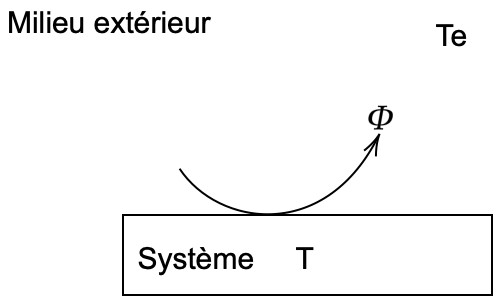
\includegraphics[scale=0.35]{figures/thermo/convection1.png}
\end{center}

\etiquette{Exemple} Plat chaud qui sort du four et qui refroidit dans l'air de la cuisine.

\etiquette{Vocabulaire}

Proche de la surface du système, le fluide touche le système. Il y a alors \textbf{conduction} mais aussi \textbf{convection} car le fluide est en mouvement. On parle de transfert \textbf{convectif} entre le fluide et la surface du système.

\blocrouge{Formule de Newton}{Le flux convectif $\Phi$ échangé entre un système à la température T et un fluide à la température Te vaut: $$\boxed{\Phi = h\times(T_e - T)\times S}$$ Unités: h est le coefficient convectif en $\SI{}{\watt\per\meter\squared\per\kelvin\squared}$ ; S: la surface du système en $m^2$ ; T et Te en K (ou\SI{}{\celsius}) et $\Phi$ en W  }


\etiquetterouge{Réfléchir au signe !}
$\Phi$ peut être positif ou négatif. Si la surface est plus chaude que l'extérieur $T_e < T$ , le flux $\Phi$ est \trou{ négatif}. Cela correspond  à une \trou{perte d'énergie} pour la surface.
On retrouve la convention de la thermodynamique et celle du banquier.
\subsection{Bilan d'énergie du système}
\etiquette{Situation}
Le système est incompressible, au repos à la température T. Il échange de l'énergie uniquement par transfert conducto-convectif avec le milieu extérieur de température Te. Condition initiale: on sait que à t=0 $T(0)=T_0$.\\

\begin{center}
	\includegraphics[scale=0.4]{figures/thermo/convection2.pdf}
\end{center}

D'après le premier principe de la thermodynamique, on a :
\trou{$\Delta U = Q$}\\
Or, $$Q=\trou{\Phi \Delta t}$$ et $$\Delta U = \trou{C.\Delta T}$$


\blocgris{A Savoir Faire}{\textbf{Etablir l'équation différentielle}. T(t) est la fonction recherchée.
\begin{align*}
	C.\Delta T &= \Phi . \Delta t & \text{Bilan\: d'énergie}\\
		C.\Delta T &=  h.(T_e-T).S .\Delta t& \text{Loi de Newton}\\
	C. \frac{\Delta T}{\Delta t} &= \Phi = h.(T_e-T).S & \text{Division par }\Delta t\\
	\text{En faisant tendre \trou{$\Delta t$ vers 0}}\\
	C.\frac{dT}{dt} &= 	h.(T_e-T).S\\
	\\
	\frac{dT}{dt} &= 	\frac{h.S}{C}(T_e-T)\\
	\\
	\boxed{\dfrac{dT}{dt}=-\dfrac{hS}{C}T + \dfrac{hS}{C}Te} & &\text{Mise sous la forme }y'=ay+b
\end{align*}
}

On obtient une équation différentielle d'ordre 1 avec second membre constant.\\

\etiquette{Solution de l'équation différentielle}

\begin{center}
\trou{$$\boxed{T(t)=Te+(T_0-Te)e^{-t/\tau}}$$}
\trou{Avec $\tau=\dfrac{C}{hS}$ le temps caractéristique de refroidissement, exprimé en seconde}
\end{center}

Vérifier que cette expression est bien solution de l'équation différentielle et que $\tau$ est bien homogène à un temps.

\begin{travail}
\begin{itemize}
	\item Asie 2024 Jour 1  \url{https://www.labolycee.org/etude-dune-bouteille-isotherme}
	\item \url{https://www.labolycee.org/preparer-un}
\item \url{https://www.labolycee.org/capacite-thermique-massique-du-cuivre}
\item \url{https://www.labolycee.org/evolution-de-la-temperature-dans-une-bouteille-isotherme}

\end{itemize}
\end{travail}

% \setcounter{chapter}{16}

\chapter{Electrolyse}
\section{Electrolyse}
\subsection{Transformation forcée}
\etiquetterouge{Idée forte} En apportant de l'énergie électrique à un système chimique, il est possible de \trou{ renverser }le sens de l'évolution spontanée d'une réaction chimique, c'est \textbf{\trou{l'électrolyse}}. L'énergie est apportée par un \textbf{générateur} qui va \textbf{\trou{imposer le sens }du courant} et donc celui des échanges d'électrons.

\subsection{Electrolyse d'une solution de chlorure d'étain}
\etiquette{Montage} Voir Florilège de chimie pratique page 257

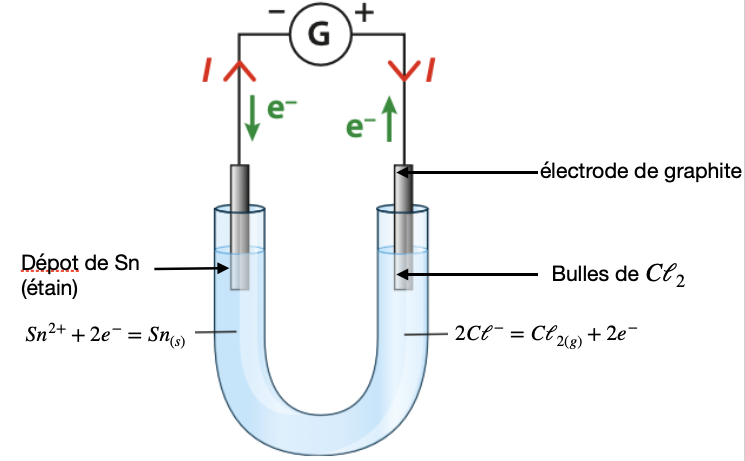
\includegraphics[width=10 cm]{figures/electrolyse_3}

Vidéo de l'expérience: \url{https://www.youtube.com/watch?v=0KI65y_b5y4}

\subsection{Obtention des équations redox}

On sait que :
\begin{itemize}
	\item Le courant I et le sens des $e^-$ est imposé par le générateur. 
	\item Initialement les seules espèces chimiques présentes sont: $C\ell^-$ et $Sn^{2+}$.
	\item Les couples sont $C\ell_{2(g)} / C\ell^-$ et $Sn^{2+} / Sn$.
	\item Equations redox des couples $$\trou{C\ell_{2(g)}} + 2e^- = \trou{C\ell^-}$$ $$Sn^{2+}+\trou{2e^-}=\trou{Sn}$$
\end{itemize}
 On en déduit que: 
\begin{itemize}
	\item Les électrons arrivent à gauche. Ils sont consommés selon $$\trou{Sn^{2+}}+2e^- = \trou{Sn}$$
	\item Les électrons qui partent de l'électrode à droite sont produits par $$2C\ell^-=C\ell_{2(g)}+\trou{2e^-}$$
\end{itemize}

\subsection{Interprétation chimique}

Durant l'électrolyse, on observe la réaction d'équation $$\trou{2C\ell^-+Sn^{2+}}\longrightarrow \trou{C\ell_{2(g)}+Sn_{(s)}}$$ 

\blocgris{Questions}{
On donne les concentrations initiales: $[Sn^{2+}]_i = 0,5$ mol/L et $[C\ell^-]_i = 1$ mol/L. Les activités du dichlore et de l'étain solide seront prises égales à 1.
\begin{enumerate}
	\item Calculer la valeur du quotient réactionnel à l'instant initial: $Q_{ri}$ ? 
	\item Sachant que la constante d'équilibre associée à la réaction ci-dessus vaut: K = \num{e-51}. Quel est le sens spontané de la réaction chimique.
	\item Justifier qu'il s'agit ici d'une réaction forcée.
\end{enumerate}
}

\etiquette{A savoir aussi... }
Les éléments des deux premières colonnes du tableau périodique sont les éléments du bloc s. Ils ont tous un ou deux électrons sur leur couche externe. Ils sont donc susceptibles de les perdre, ce qui fait d'eux des \trou{réducteurs}

\etiquette{Récap du cours sur électrolyse} \url{https://www.youtube.com/watch?v=w3lg9HDBMKw}


\newpage
\section{Application : dépôt d'un métal sur une surface}
L'un des procédés utilisé pour protéger l'acier de la corrosion est de l'isoler de l'atmosphère en le recouvrant
d'un revêtement métallique. Des plaques d'acier sont ainsi recouvertes d'une fine couche de zinc, on dit
qu'elles sont « galvanisées ».
Pour cela, on procède à l'électrolyse d'une solution aqueuse de sulfate de zinc (II) ($Zn^{2+}_{(aq)} + SO4
^{2-}_{4(aq)}$).
Dans ce bain électrolytique, on plonge une plaque à recouvrir et on utilise une lame de zinc comme seconde
électrode

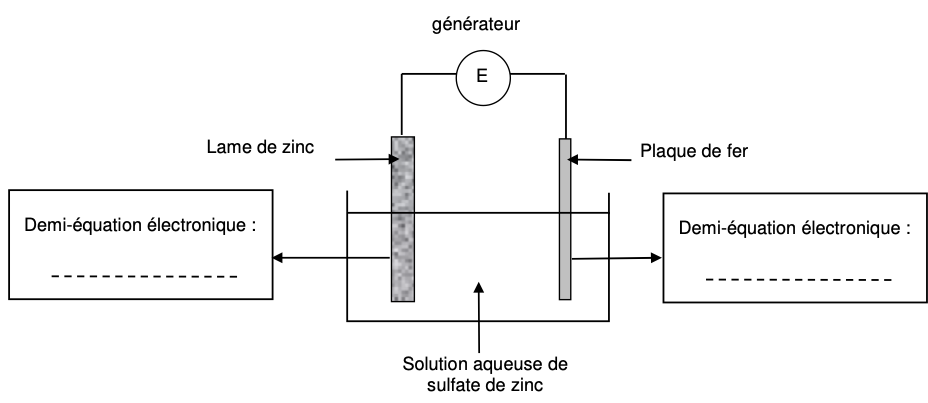
\includegraphics[width=12 cm]{figures/electrolyse_4.png}

\etiquette{Questions}
\begin{enumerate}
\item Compléter le schéma précédent en indiquant: où se forme le dépôt de zinc, la demi équation électronique traduisant la transformation ayant lieu sur la plaque de fer ($Fe^{2+}/Fe$);
\begin{itemize}
\item le sens de déplacement des électrons dans les conducteurs métalliques ;
\item les polarités du générateur ;
\item la demi équation électronique traduisant la transformation ayant lieu sur la lame de zinc.
\end{itemize}
La plaque d'acier a une surface totale de \SI{10}{m^2}. On veut déposer une couche de zinc de 0,10 mm
d'épaisseur, ce qui correspond à un volume de zinc égal à 1000 cm3. L'intensité du courant est maintenue
constante et égale à 1,0 kA.
\item  Calculer la masse de zinc à déposer.
\item En déduire la quantité d'électrons en mol devant traverser le circuit.
\item En déduire la durée de l'électrolyse.
\end{enumerate}
Données
\begin{itemize}
\item Masse volumique du zinc:$\rho=7,14g.cm^{-3}$
\item Masse molaire du zinc: M =65,4g/mol
\item Constante d'Avogadro: $ N_{A}=6,02\times10^{23}mol^{-1}$
\item Charge élémentaire: $e=1,60\times10^{-19}\:C$ 
\item Faraday: F=$96500\:C.mol^{-1}$
\end{itemize}
%\blocgris{Demi-équations}{
%Pour chacun des couples ci-dessous, écrire la demi-équation d'oxydo-réduction : 
%\begin{itemize}
%\item L'eau de javel est une solution d'ion hypochlorite $ClO^-$ oxydant du couple : $ClO^-/Cl^-$\\
%\trou{$ClO^-+H_20+2e-=Cl^-+2HO^-$}
%\item le dioxygène $O_2$ est l'oxydant du couple $O_2/H_2O$\\
%\trou{$O_2+4e-+4H^+=2H_2O$}
%\item le dichlore $Cl_2$ est l'oxydant du couple $Cl_2/Cl^-$\\
%\trou{$Cl_2+2e-=2Cl^-$}
%\item l'acide ascorbique ou vitamine C est le réducteur du couple $C_6H_6O_6/C_6H_8O_6$\\
%\trou{$C_6H_6O_6 +2H^+  = C_6H_8O_6$}
%\item le dihydrogène $H_2$ est le réducteur du couple $H^+/H_2$.\\
%\trou{$2H^+ +2e-=H_2$}
%\end{itemize}
%}

\etiquette{Exercices sur l'électrolyse}
\begin{itemize}
\item 1, 2, 8, 12 et 18 p 184
\item type bac: \url{https://www.labolycee.org/corrosion-et-protection-des-metaux}
\end{itemize}
% \setcounter{chapter}{18}
\chapter{Lunette Astronomique}
\section{Constructions Fondamentales}
\subsection{Construction de l'image de l'objet AB}

\blocrouge{Vocabulaire et Règles}{
\begin{itemize}
\item O est le \trou{centre optique de la lentille.}
\item F est le \trou{foyer principal objet de la lentille.}
\item F' est le \trou{foyer principal image de la lentille.}
\item $OF=OF'$ désigne la distance focale en mètre. $v=\frac{1}{f'}$ est la vergence de la lentille en \trou{dioptrie noté : $\delta$}
\end{itemize}
\begin{enumerate}
	\item Tout rayon parallèle à l'axe optique émerge en \trou{passant par le foyer image F'}
	\item Tout rayon incident passant par le centre O émerge de la lentille \trou{sans être dévié.}
	\item Tout rayon incident passant par le foyer F émerge \trou{parallèlement à l'axe optique.}
\end{enumerate}
}

\etiquette{Schéma important}: Construction de l'image d'un objet AB par une lentille (L) 


\includegraphics{figures/lunette/rappel_1}

\etiquette{Consignes} En utilisant 3 rayons particuliers émis par B, construire son image B'. En déduire l'image A'B' produite par la lentille.

\subsection{Objet à l'infini}
Eloignons progressivement un point lumineux B et observons l'inclinaison des rayons qui entrent dans la lentille. \\

\includegraphics{figures/lunette/lunette_01}

On observe que plus B est loin de la lentille, plus l'angle entre les rayons qui pénètrent dans la lentille est petit. \\ A la limite lorsque B est infiniment à gauche sur la figure, cet angle devient nul  et les rayons qui pénètrent dans la lentille sont parallèles.

\blocrouge{Propriété 1}{
Un point \textbf{objet situé à l'infini} est représenté par une collection de \trou{\textbf{rayons lumineux parallèles} entre eux.}}

\etiquette{Construction 1} Objet B situé à \trou{l'infini}
\\
%version prof
%\includegraphics[scale=.75]{figures/lunette/lunette_02}
%version élève
\includegraphics{figures/lunette/lunette_03} 
\\
\etiquette{Stratégie de construction}: 
\begin{enumerate}
	\item Tracer le rayon passant par O
	\item Repérer l'intersection entre ce rayon et le plan focal: c'est B'
	\item Tous les rayons émis par $B_\infty$ sortent de la lentille en passant par B'
\end{enumerate}
\etiquetterouge{On retient} L'image d'un objet AB situé à l'infini est située dans \trou{\textbf{le plan focal image}} de la lentille.

\subsection{Objet situé dans le plan focal objet}
\etiquette{Construction 2}\\
%version prof
%\includegraphics[scale=.75]{figures/lunette/lunette_04}
%version élève
\includegraphics[scale=.75]{figures/lunette/lunette_05}
\\

\etiquette{Stratégie de construction}
\begin{enumerate}
	\item Tracer le rayon passant par O qui n'est pas dévié.
	\item Tracer le rayon émis par B et parallèle à l'axe optique, il sort en passant par F'
	\item Tous les rayons émis par B sortent de la lentille selon des rayons parallèles aux deux premiers tracés.
\end{enumerate}
\etiquetterouge{On retient} L'image d'un objet AB situé dans le plan focal objet de la lentille est situé à \textbf{l'infini}. C'est à dire que les rayons émergent \trou{parallèlement entre eux. } L'oeil voit dans le prolongement \trou{des rayons qu'il reçoit}.

\section{Présentation de la lunette astronomique}
\subsection*{Un peu d'histoire}
La lunette astronomique a été mise au point par Johannes Kepler en 1611 pour observer les astres ou les objets très éloignés. Il a repris la lunette de Galilée mise au point au siècle précédent et l'a améliorée.\\

\etiquette{Intérêt de la lunette}\\
La lunette astronomique a pour but d'observer des objets à l'infini, et de les grossir afin qu'ils soient observés par un \oe il sans accommodation (sans effort comme quand on regarde au loin). \\
Pour que l'\oe il n'accommode pas, l'image à la sortie de la lentille doit être formée à l'infini.\\
La lunette astronomique donne donc d'un objet à l'infini une image à l'infini, c'est ce que l'on appelle un dispositif \trou{afocal} (c'est à dire ne comportant pas de foyer).

\etiquette{Anatomie}\\
La lunette astronomique est constituée de \trou{Deux lentilles convergentes} :\\
\begin{minipage}{0,65\linewidth}
\begin{itemize}
\item \textbf{L'objectif} : Il se trouve du côté de \trou{l'objet} que l'on souhaite observer.\\
Il forme d'un objet $A_\infty B_\infty$ à l'infini une image $A_1B_1$ dans le plan focal image.\\
 Il est modélisé par une lentille convergente, notée $L_1$, de distance focale $f'_1$

\vspace{1,5cm}
\item \textbf{L'oculaire} : Il se trouve du côté de \trou{l'oeil}.\\
Il forme d'un objet $A_1B_1$ situé dans le plan focal objet une image à l'infini $A'_\infty B'_\infty$.\\
il est modélisé par une lentille convergente, de distance focale $f'_2$.
\end{itemize}
\end{minipage}
\begin{minipage}{0,3\linewidth}
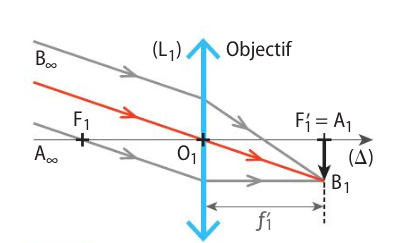
\includegraphics[scale=0.4]{figures/lunette/fig_obj}
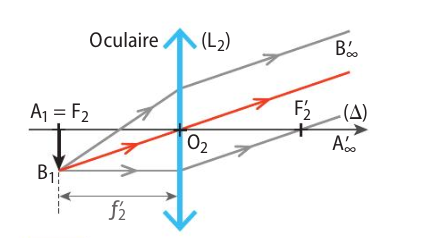
\includegraphics[scale=0.4]{figures/lunette/fig_oc}
\end{minipage}


Pour que la lunette soit afocale, il faut que \trou{le plan focal image de l'objectif} soit confondu avec \trou{le plan focal objet de l'oculaire.}\\

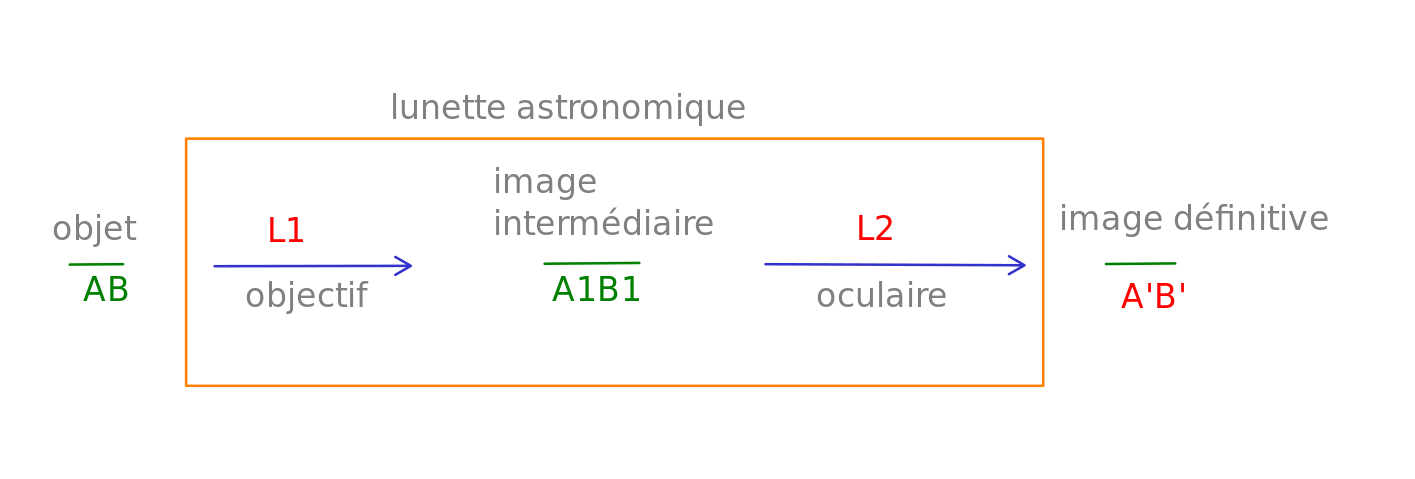
\includegraphics[scale=0.3]{figures/lunette/fig_modele}\\


\section{Construction du faisceau traversant une lunette afocale}
\etiquetterouge{Objectif} Tracer (sur le schéma incomplet qui suit)  le trajet des rayons émis par un objet AB situé à l'infini de la lentille. On doit obtenir la construction suivante:\\
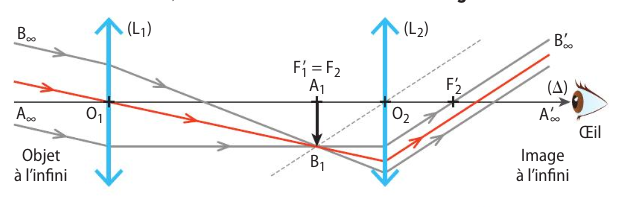
\includegraphics[scale=0.7]{figures/lunette/fig_lunette}\\
\includegraphics{figures/lunette/lunette_07}

%\newpage

\blocrouge{Entraînement à la Maison}{

Représenter, à l'échelle $\dfrac{1}{5}$ le modèle de la lunette astronomique suivante : \begin{itemize}
\item L'objectif est une lentille convergente de distance focale $f'_1=\SI{50}{\centi\meter}$
\item L'oculaire est une lentille convergente de distance focale $f'_2=\SI{10}{\centi\meter}$
\end{itemize}
Tracer le trajet de rayons lumineux issus d'un objet situé à l'infini, rayons faisant un angle $\alpha$ avec l'axe optique, à travers la lunette astronomique.\\ On notera $\alpha '$ l'angle fait par les rayons émergents avec l'axe optique.
}

\vspace{2cm}

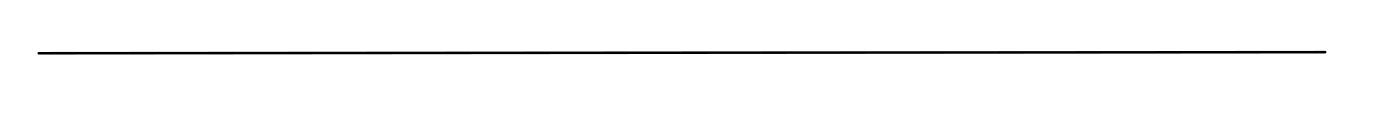
\includegraphics[scale=0.4]{figures/lunette/axe}

\vspace{2cm}
\newpage
\section{Grossissement}
\subsection{Grossissement G d'un système afocal}
Le grossissement noté G est une grandeur sans unité liée aux angles sous lesquels on observe l'objet à l'\oe il nu et son image à travers la lunette.\\

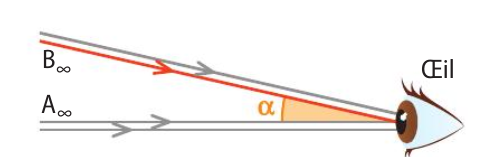
\includegraphics[scale=0.5]{figures/lunette/alpha}
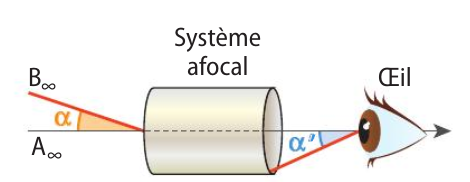
\includegraphics[scale=0.5]{figures/lunette/alpha'}\\
A travers la lunette, on voit l'astre comme s'il était situé à une distance plus petite que la distance réelle. Donc, l'angle $\alpha'$ est plus grand que l'angle $\alpha$.

\blocrouge{Définition}{
On définit le grossissement comme étant 
$$\trou{\boxed{G=\dfrac{\alpha'}{\alpha}}}$$

avec $\alpha'$ l'angle sous lequel l'image définitive A'B' est vue à travers la lunette\\
Et $\alpha$ l'angle sous lequel l'objet AB est vu à l'\oe il nu.
}


\subsection{Calcul de G pour la lunette astronomique}
\etiquette{Stratégie}
\begin{enumerate}
	\item Calculer $\tan\alpha$ et $\tan\alpha '$ dans un triangle dont un des côtés est $A_1B_1$.
	\item Faire l'approximation des petits angles: $\tan\alpha\approx\alpha$
	\item Calculer $G=\dfrac{\alpha '}{\alpha}$ 
\end{enumerate}
\begin{minipage}{0,4\linewidth}
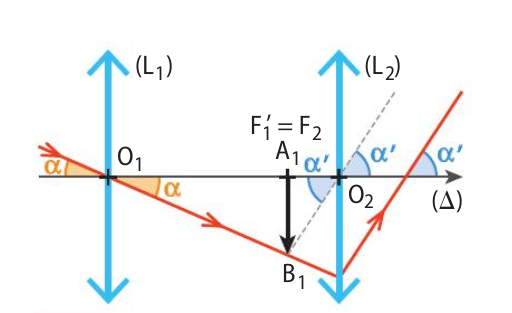
\includegraphics[scale=0.4]{figures/lunette/grossissement}
\end{minipage}
\begin{minipage}{0,6\linewidth}
Dans le triangle $O_1A_1B_1$, on a $\tan \alpha =$
\end{minipage}
\newpage
\etiquetterouge{Votre Synthèse}

\tikzset{every picture/.style={line width=0.75pt}} %set default line width to 0.75pt        

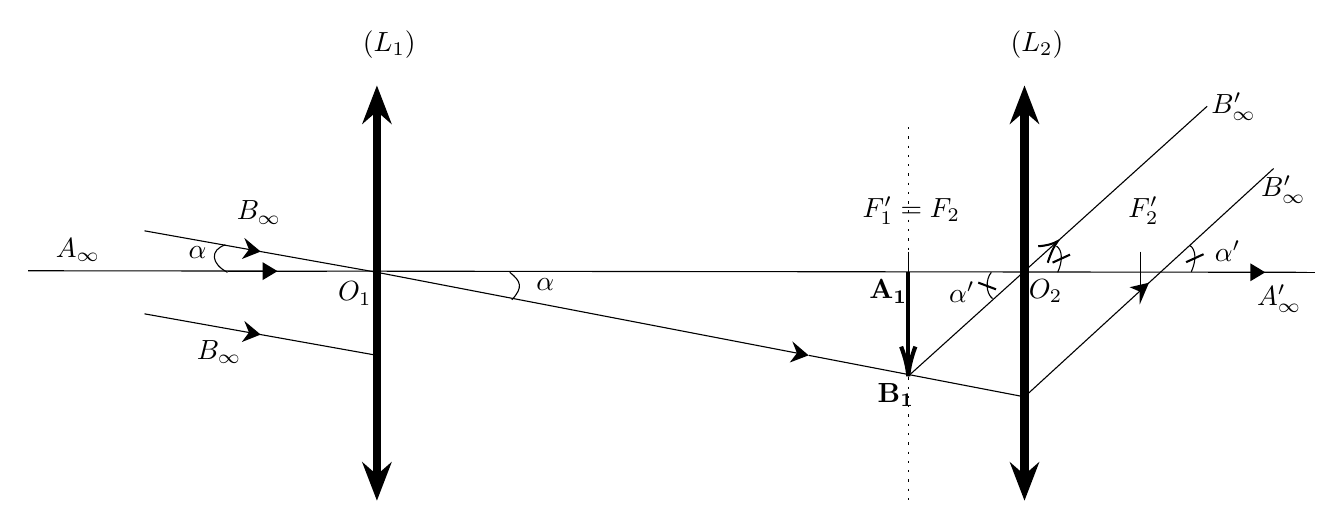
\begin{tikzpicture}[x=0.75pt,y=0.75pt,yscale=-1,xscale=.8]
%uncomment if require: \path (0,300); %set diagram left start at 0, and has height of 300

%Straight Lines [id:da2168956321390959] 
\draw    (-65,129.25) -- (705,130) ;
%Straight Lines [id:da11173057992958146] 
\draw [line width=3]    (145,46) -- (145,234) ;
\draw [shift={(145,240)}, rotate = 270] [fill={rgb, 255:red, 0; green, 0; blue, 0 }  ][line width=0.08]  [draw opacity=0] (18.75,-9.01) -- (0,0) -- (18.75,9.01) -- (12.45,0) -- cycle    ;
\draw [shift={(145,40)}, rotate = 90] [fill={rgb, 255:red, 0; green, 0; blue, 0 }  ][line width=0.08]  [draw opacity=0] (18.75,-9.01) -- (0,0) -- (18.75,9.01) -- (12.45,0) -- cycle    ;
%Straight Lines [id:da7566910966643488] 
\draw    (465,120) -- (465,140) ;
%Straight Lines [id:da6357288075561843] 
\draw [line width=3]    (535,46) -- (535,234) ;
\draw [shift={(535,240)}, rotate = 270] [fill={rgb, 255:red, 0; green, 0; blue, 0 }  ][line width=0.08]  [draw opacity=0] (18.75,-9.01) -- (0,0) -- (18.75,9.01) -- (12.45,0) -- cycle    ;
\draw [shift={(535,40)}, rotate = 90] [fill={rgb, 255:red, 0; green, 0; blue, 0 }  ][line width=0.08]  [draw opacity=0] (18.75,-9.01) -- (0,0) -- (18.75,9.01) -- (12.45,0) -- cycle    ;
%Straight Lines [id:da9852783124894242] 
\draw    (605,120) -- (605,140) ;
%Straight Lines [id:da3109976381088303] 
\draw    (275,150) -- (145,130) ;
%Straight Lines [id:da8566852525579076] 
\draw    (402.03,169.54) -- (275,150) ;
\draw [shift={(405,170)}, rotate = 188.75] [fill={rgb, 255:red, 0; green, 0; blue, 0 }  ][line width=0.08]  [draw opacity=0] (10.72,-5.15) -- (0,0) -- (10.72,5.15) -- (7.12,0) -- cycle    ;
%Straight Lines [id:da7648211303216299] 
\draw    (535,190) -- (405,170) ;
%Straight Lines [id:da35136732445197005] 
\draw  [dash pattern={on 0.84pt off 2.51pt}]  (465,60) -- (465,240) ;
%Straight Lines [id:da8597413149358359] 
\draw    (465,180) -- (645,50) ;
\draw [shift={(555,115)}, rotate = 144.16] [color={rgb, 255:red, 0; green, 0; blue, 0 }  ][line width=0.75]    (10.93,-4.9) .. controls (6.95,-2.3) and (3.31,-0.67) .. (0,0) .. controls (3.31,0.67) and (6.95,2.3) .. (10.93,4.9)   ;
%Straight Lines [id:da274094382380242] 
\draw    (535,190) -- (685,80) ;
\draw [shift={(610,135)}, rotate = 143.75] [fill={rgb, 255:red, 0; green, 0; blue, 0 }  ][line width=0.08]  [draw opacity=0] (10.72,-5.15) -- (0,0) -- (10.72,5.15) -- (7.12,0) -- cycle    ;
%Straight Lines [id:da847708984830482] 
\draw    (5,110) -- (145,130) ;
\draw [shift={(75,120)}, rotate = 188.13] [fill={rgb, 255:red, 0; green, 0; blue, 0 }  ][line width=0.08]  [draw opacity=0] (10.72,-5.15) -- (0,0) -- (10.72,5.15) -- (7.12,0) -- cycle    ;
%Straight Lines [id:da02702840130814277] 
\draw    (5,150) -- (145,170) ;
\draw [shift={(75,160)}, rotate = 188.13] [fill={rgb, 255:red, 0; green, 0; blue, 0 }  ][line width=0.08]  [draw opacity=0] (10.72,-5.15) -- (0,0) -- (10.72,5.15) -- (7.12,0) -- cycle    ;
%Curve Lines [id:da5961926220635629] 
\draw    (53.75,116.75) .. controls (44.33,119.22) and (45,125.89) .. (55,130) ;
%Curve Lines [id:da23585236461317316] 
\draw    (225,130) .. controls (231.75,134.25) and (233.25,137.25) .. (226.25,143.25) ;
%Straight Lines [id:da4781405060937802] 
\draw [line width=1.5]    (465,130) -- (465,177) ;
\draw [shift={(465,180)}, rotate = 270] [color={rgb, 255:red, 0; green, 0; blue, 0 }  ][line width=1.5]    (14.21,-4.28) .. controls (9.04,-1.82) and (4.3,-0.39) .. (0,0) .. controls (4.3,0.39) and (9.04,1.82) .. (14.21,4.28)   ;
%Curve Lines [id:da5186850592414963] 
\draw    (515,130) .. controls (511.36,133.55) and (511.73,140.18) .. (515.73,142.64) ;
\draw [shift={(512.49,136.58)}, rotate = 286.77] [color={rgb, 255:red, 0; green, 0; blue, 0 }  ][line width=0.75]    (0,5.59) -- (0,-5.59)   ;
%Curve Lines [id:da359362515174557] 
\draw    (554.27,117.36) .. controls (557.86,119.29) and (558.14,124.43) .. (555,130) ;
\draw [shift={(557.16,123.41)}, rotate = 249.91] [color={rgb, 255:red, 0; green, 0; blue, 0 }  ][line width=0.75]    (0,5.59) -- (0,-5.59)   ;
%Curve Lines [id:da2510289125381956] 
\draw    (634.71,117.14) .. controls (638.3,119.06) and (638.58,124.21) .. (635.44,129.78) ;
\draw [shift={(637.6,123.19)}, rotate = 249.91] [color={rgb, 255:red, 0; green, 0; blue, 0 }  ][line width=0.75]    (0,5.59) -- (0,-5.59)   ;
%Straight Lines [id:da10265543314732706] 
\draw    (55.14,129.43) -- (115.14,129.43) ;
\draw [shift={(85.14,129.43)}, rotate = 180] [fill={rgb, 255:red, 0; green, 0; blue, 0 }  ][line width=0.08]  [draw opacity=0] (8.93,-4.29) -- (0,0) -- (8.93,4.29) -- cycle    ;
%Straight Lines [id:da7876984232434279] 
\draw    (650,130) -- (710,130) ;
\draw [shift={(680,130)}, rotate = 180] [fill={rgb, 255:red, 0; green, 0; blue, 0 }  ][line width=0.08]  [draw opacity=0] (8.93,-4.29) -- (0,0) -- (8.93,4.29) -- cycle    ;

% Text Node
\draw (436,92.4) node [anchor=north west][inner sep=0.75pt]    {$F'_{1} =F_{2}$};
% Text Node
\draw (135,12.4) node [anchor=north west][inner sep=0.75pt]    {$( L_{1})$};
% Text Node
\draw (120,133.4) node [anchor=north west][inner sep=0.75pt]    {$O_{1}$};
% Text Node
\draw (536,132.4) node [anchor=north west][inner sep=0.75pt]    {$O_{2}$};
% Text Node
\draw (596,92.4) node [anchor=north west][inner sep=0.75pt]    {$F'_{2}$};
% Text Node
\draw (525,12.4) node [anchor=north west][inner sep=0.75pt]    {$( L_{2})$};
% Text Node
\draw (59,94.4) node [anchor=north west][inner sep=0.75pt]    {$B_{\infty }$};
% Text Node
\draw (35,161.4) node [anchor=north west][inner sep=0.75pt]    {$B_{\infty }$};
% Text Node
\draw (30,116.4) node [anchor=north west][inner sep=0.75pt]    {$\alpha $};
% Text Node
\draw (239.5,131.9) node [anchor=north west][inner sep=0.75pt]    {$\alpha $};
% Text Node
\draw (445,182.4) node [anchor=north west][inner sep=0.75pt]    {$\mathbf{B_{1}}$};
% Text Node
\draw (440,132.4) node [anchor=north west][inner sep=0.75pt]    {$\mathbf{A_{1}}$};
% Text Node
\draw (488,133.4) node [anchor=north west][inner sep=0.75pt]    {$\alpha '$};
% Text Node
\draw (648,113.4) node [anchor=north west][inner sep=0.75pt]    {$\alpha '$};
% Text Node
\draw (646,42.4) node [anchor=north west][inner sep=0.75pt]    {$B'_{\infty }$};
% Text Node
\draw (676,82.4) node [anchor=north west][inner sep=0.75pt]    {$B'_{\infty }$};
% Text Node
\draw (-50,112.4) node [anchor=north west][inner sep=0.75pt]    {$A_{\infty }$};
% Text Node
\draw (673.5,134.9) node [anchor=north west][inner sep=0.75pt]    {$A'_{\infty }$};


\end{tikzpicture}


\etiquetterouge{Exercices}

\begin{itemize}
	\item Reconnaître le montage: 2, 3 p 396
	\item Tracer des rayons: 5, 6 , 9 p 397
	\item Calculs classiques: 11 et 12 p 398
	\item Préparer le bac: 24, 25 p 403
 	\item TYPE BAC: \url{https://labolycee.org/observation-ornithologique-dune-oie-cendree}
\end{itemize}
% \setcounter{chapter}{18}
\chapter{Effet photoélectrique}
\section{Le photon}
\subsection{Modèle onde - corpuscule}


\blocrouge{Rappels}{Le photon est une \trou{particule} (ou corpuscule) de masse \trou{nulle}. Le photon est la particule associée à un rayonnement électromagnétique. 

Jusqu'ici le rayonnement a été décrit par une \trou{onde}. Dans ce chapitre, il est décrit comme \trou{un flux} de photons.

Une onde électromagnétique se propageant dans le vide est décrit par une longueur d'onde $\lambda$ en m , une fréquence $\nu$ en \si{\per \second} et une vitesse de propagation $c=\SI{3.0e8}{\meter\per\second}$ 

On a alors $$\nu=\trou{\frac{c}{\lambda}}$$

}
\subsection{Energie d'un photon}

Chaque photon transporte une quantité d'énergie: E. Cette énergie est proportionnelle à la \trou{fréquence} du rayonnement (de l'onde) 

\blocrouge{Formule}{L'énergie d'un photon de fréquence $\nu$ vaut $$E=\trou{h\times \nu}$$
E en J ; $\nu$ la fréquence de l'onde en Hz ou \si{\per\second}\\ h=$\SI{6.63e-34}{\joule\per\second}$ est la constante de Planck 

}

\etiquette{Applications}
\begin{enumerate}
	\item Calculer la fréquence d'un photon violet $\lambda=\SI{400}{\nano\meter}$ et d'un photon rouge $\lambda=\SI{800}{\nano\meter}$ 
	\item Représenter sur un axe de longueur d'onde le domaine du visible et nommer les domaines voisins.
	\item Ajouter un axe correspondant à la fréquence des ondes électromagnétiques. Comment est-il orienté par rapport à l'axe en longueur d'onde ?
	\item Calculer en joules  l'énergie d'un photon violet et d'un photon rouge.
\end{enumerate}


\section{Effet photoélectrique}
\subsection{Description de l'expérience}
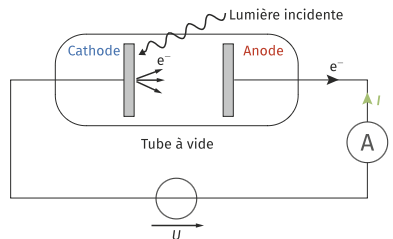
\includegraphics[width=.6\textwidth]{figures/effet_photoelectrique}\\
\url{https://phet.colorado.edu/sims/cheerpj/photoelectric/latest/photoelectric.html?simulation=photoelectric&locale=fr}\\
On éclaire en lumière monochromatique une plaque métallique. 

\blocrouge{Définition}{L'effet photoélectrique est le phénomène qui consiste en \trou{l'émission} d'électrons (courant électrique) par un matériau qui reçoit \trou{un rayonnement électromagnétique.}}

\subsection{Observations}
\begin{itemize}
	\item Pour certaines fréquences, on observe que la plaque émet \trou{des électrons}. 
	\item Il existe une fréquence \trou{seuil} en dessous de laquelle il ne se produit plus d'effet photoélectrique. 
	\item Même en augmentant l'intensité du rayonnement, si la fréquence est sous le seuil on \trou{n'observe pas }d'effet photoélectrique.
\end{itemize}

\subsection{Explications}

\begin{itemize}
	\item Les électrons de la plaque sont liés aux atomes par des forces \trou{attractives} (noyaux chargés +).
	\item En apportant une quantité d'énergie appelée \trou{travail d'extraction }(noté $W_{extraction}$) un électron est libéré de la plaque.
	\item Si l'énergie apportée par le photon est supérieure à $W_{extraction}$ alors l'excédant est \trou{emporté} par l'électron sous forme d'\trou{énergie cinétique}.
	\item L'énergie cinétique de l'électron lui permet de rejoindre l'anode et se traduit par un courant électrique que mesure \trou{l'ampèremètre}.
\end{itemize}

\blocrouge{Bilan énergétique}
{
 L'énergie d'un photon incident est utilisée pour extraire un électron et lui donner une énergie cinétique.\\
 Ecrivons la conservation de l'énergie:
 $$h\times \nu =\trou{W_{extraction}} + \trou{\frac{1}{2}m\times v^2} $$
}

\etiquette{Application}

Un photon d'énergie $Ec=\SI{5.03}{\eV}$ extrait un électron depuis une plaque de fer métallique. 
\begin{enumerate}
	\item Ecrire le bilan énergétique de cette situation.
	\item Calculer en joule, l'énergie cinétique maximale de l'électron arraché.
\end{enumerate}
On donne: $\SI{1}{\eV}=\SI{1.6e-19}{\J}$, pour un électron d'un atome de fer: $W_{extraction}=\SI{4.76}{\eV}$

\vspace{7cm}
\subsection{Ceci est une révolution !}

C'est l'interprétation de l'effet photoélectrique qui a permis de valider l'idée \trou{d'Einstein} selon laquelle l'interaction onde matière peut se décrire à l'aide d'une particule: le \trou{photon}. 

En effet, la description ondulatoire de la lumière ne peut rendre compte des résultats expérimentaux de l'expérience schématisée plus haut. Einstein obtient le prix \trou{Nobel} pour cette explication de l'effet photoélectrique par le photon. Cela marque le début de la \trou{mécanique quantique}.

%Lecture pour aller plus loin \url{https://query.libretexts.org/Francais/Physique_universitaire_III_-_Optique_et_physique_moderne_%28OpenStax%29/06%3A_Photons_et_ondes_de_matière/6.03%3A_Effet_photoélectrique}

\section{Absorption et Emission de photons}
\subsection{Absorption de photon}
\etiquette{Panneau photovoltaïque}

La surface d'un panneau photovoltaïque est constituée de cellules photovoltaïques. Chacune de ces cellules absorbe des photons et par effet photoélectrique produit un \trou{courant}.

Le rendement $\eta$ d'une cellule est le rapport entre la puissance électrique \trou{produite} et la puissance du rayonnement \trou{reçue}. $$\eta=\frac{\mathcal{P}_{elec}}{\mathcal{P}_{rayonnement}}$$

\etiquette{Capteur de lumière}

Dans un appareil photo (camera, téléphone, etc) le capteur est une surface tapissée de photodiodes. Chaque photodiode convertit la lumière reçue en courant électrique grâce à \trou{l'effet photoélectriqu}e.

\subsection{Emission de photon}
\etiquette{DEL Diode ElectroLuminescente}

Lorsque les électrons des atomes d'une DEL sont excités (par l'énergie électrique reçue) ils se désexcitent en émettant des photons. L'énergie de ces photons est liée au matériau qui constitue la DEL. 

\etiquetterouge{Exercices}

13, 14, 15 et 17 p 419
\\ \textbf{Préparer le bac} : 20 p 420

%\setcounter{chapter}{20}
\chapter{Synthèse Organique (partie 1)}
\section{Optimisation d'une étape de synthèse}
\subsection{Rappels}

On a décrit les réactions chimiques suivant deux aspects:
\begin{itemize}
	\item cinétique: influence des facteurs cinétiques (\trou{température}, \trou{catalyseur})
	\item rendement: c'est le rapport entre la quantité de produit expérimentalement produit et la quantité de produit que l'on produirait si la \trou{réaction était totale}.\
\end{itemize}
\blocrouge{A SAVOIR}{
Il y a deux techniques permettant d'augmenter le rendement d'une réaction:
\begin{enumerate}
	\item Introduire un \trou{réactif en excès}.
	\item Eliminer un \trou{produit} au fur et à mesure de se formation dans le milieu réactionnel.
\end{enumerate}
}
\subsection{Application}

On considère une réaction d'estérification (synthèse d'un ester). 
\begin{center}
	alcool + acide $\leftrightharpoons$ ester + eau
\end{center}

Cette réaction est un équilibre dont la constante vaut K=4,00. Les réactifs et produits sont en phase liquide. On assimilera leurs activités à leurs quantités de matière.

\etiquette{Protocole expérimental}
On introduit dans un ballon:

\begin{minipage}{.60\textwidth}

\begin{itemize}
	\item 8,5 mL d'acide éthanoïque ;
	\item 21,4 mL de 3-méthylbutan-1-ol ;
	\item 10 mL de cyclohexane ;
\end{itemize}
On réalise le montage de \trou{Dean-Stark} avec  la colonne graduée remplie de cyclohexane. On règle le chauffage au maximum. On arrête le chauffage lorsque 2,2 mL de liquide ont été recueillis en dessous du cyclohexane dans la colonne du Dean-Stark. Le cyclohexane et l'eau ne sont  pas miscibles.

\end{minipage}
\hfill
\begin{minipage}{.35\textwidth}
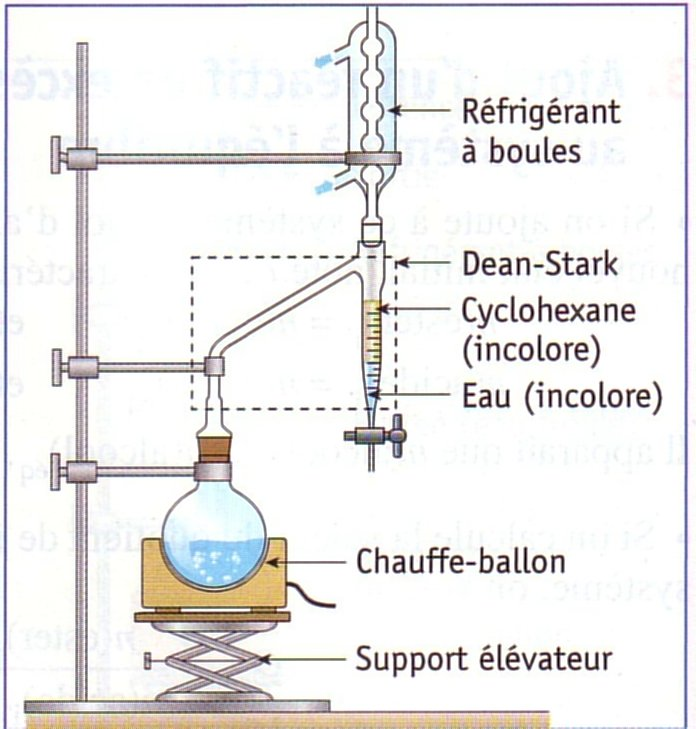
\includegraphics{figures/dean_stark}
\end{minipage}





\begin{tabular}{|l|c|c|c|c|c|}
\hline
Données &Acide éthanoïque & 3-méthylbutan-1-ol &Ester&cyclohexane & Eau\\
  \hline
  Masse molaire en g/mol & 60&88 &130 &78 &18\\
Densité  &1.05 &0.81 &0.87 & 0.88 & 1.00 \\
$\theta_{ebullition}$ & 118 & 138 & 142 & 81 & 100 \\
\hline
\end{tabular}

\etiquette{Questions}
\begin{enumerate}
	\item Déterminer les quantités de matières des deux réactifs à l'état initial. (Solution: $n_{acide}=\SI{149}{\milli \mol}$ ;  $n_{alcool}=\SI{197}{\milli \mol}$)
	\item Calculer la quantité maximale $n_{max}$ d'eau formée. (Solution: $n_{max}=\SI{149}{\milli \mol}$ )
	\item En déduire la valeur du rendement de cette réaction avec extraction de l'eau.  ($\eta = .82 = 82\%$)
	\item Déterminer l'avancement final $x_f$ de la transformation si elle avait lieu  sans extraction. (Solution: $x_f=\SI{112}{\milli\mol}$)
	\item Calculer le rendement sans extraction. (Solution: $75\%$)
	\item Pourquoi parle-t-on de déplacement d'équilibre lorsque l'on retire l'eau à l'aide de la colonne de Dean-Stark ?
\end{enumerate}

\etiquette{Vidéo du montage}
\url{https://youtu.be/_zbHeEtRTZw?si=klHvdfqU5bZK3eoG}
%\newpage

\section{Stratégie de synthèse multi-étapes}
\subsection{Grands types de réactions}

Parmi les 5 types de réaction, on connaît déjà: 
\begin{itemize}
	\item \trou{Oxydoréduction}: échange d'électrons
	\item \trou{Acide-base}: échange de protons ($H^+$)
\end{itemize}
En voici 3 autres:

\etiquette{Addition} Une molécule qui possède une \trou{double liaison} et s'associe avec une autre molécule pour réagir.

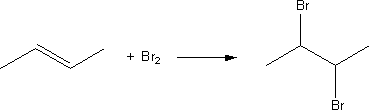
\includegraphics[scale=.80]{figures/addition}

\etiquette{Elimination} Une molécule se  scinde en deux dont l'une possède un \trou{double liaison}.

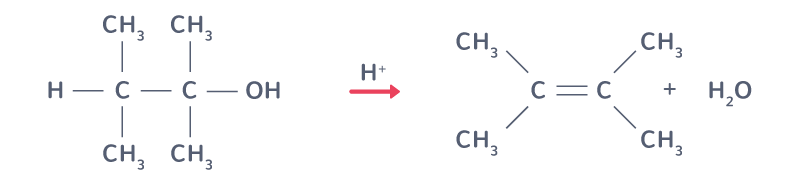
\includegraphics[scale=.40]{figures/elimination}

\etiquette{Substitution} Un atome ou un groupe d'atomes d'une molécule est \trou{remplacée} par un autre atome ou groupe d'atomes.

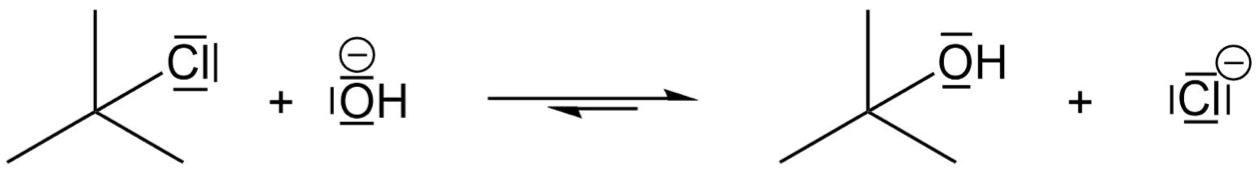
\includegraphics[scale=.450]{figures/substitution}

\subsection{Protection - Déprotection}

On considère une molécule avec plusieurs groupes fonctionnels susceptibles de réagir face à un réactif. On peut bloquer la réactivité d'un de ces groupes en réalisant la séquence suivante:

\begin{enumerate}
	\item \trou{Protection} du groupement pour lequel on ne souhaite pas de transformation chimique ;
	\item Action du réactif sur la molécule dont un groupement est protégée ; 
	\item \trou{Déprotection}: réaction permettant de régénérée le groupe fonctionnel initialement modifié par la réaction de protection.
\end{enumerate}

\etiquette{Exemple} Exercice 28 p 207

\begin{minipage}{.45\textwidth}
  On étudie la synthèse multi-étapes de B' à partir du réactif A. Pour cela, on doit modifier le groupe ester en groupe hydroxyle sans faire réagir le groupe cétone. 
\begin{enumerate}
	\item Quels sont  les groupes présents dans la molécule A. Comment se nomme ce type de composé ?
	\item Les réactifs $LiAlH_4$ et $NaBH_4$ ont ils les mêmes effets sur la molécule A ?
	\item Comment  se nomme l'étape 1 ? Quel est son intérêt ?
	\item Comment se nomme l'étape 3  ?
	\item Quel
\end{enumerate}  
  \end{minipage}
\hfill
\begin{minipage}{.55\textwidth}
\includegraphics[width=\textwidth]{figures/Exoprotection.pdf}
\end{minipage}


\subsection{Chimie Verte}

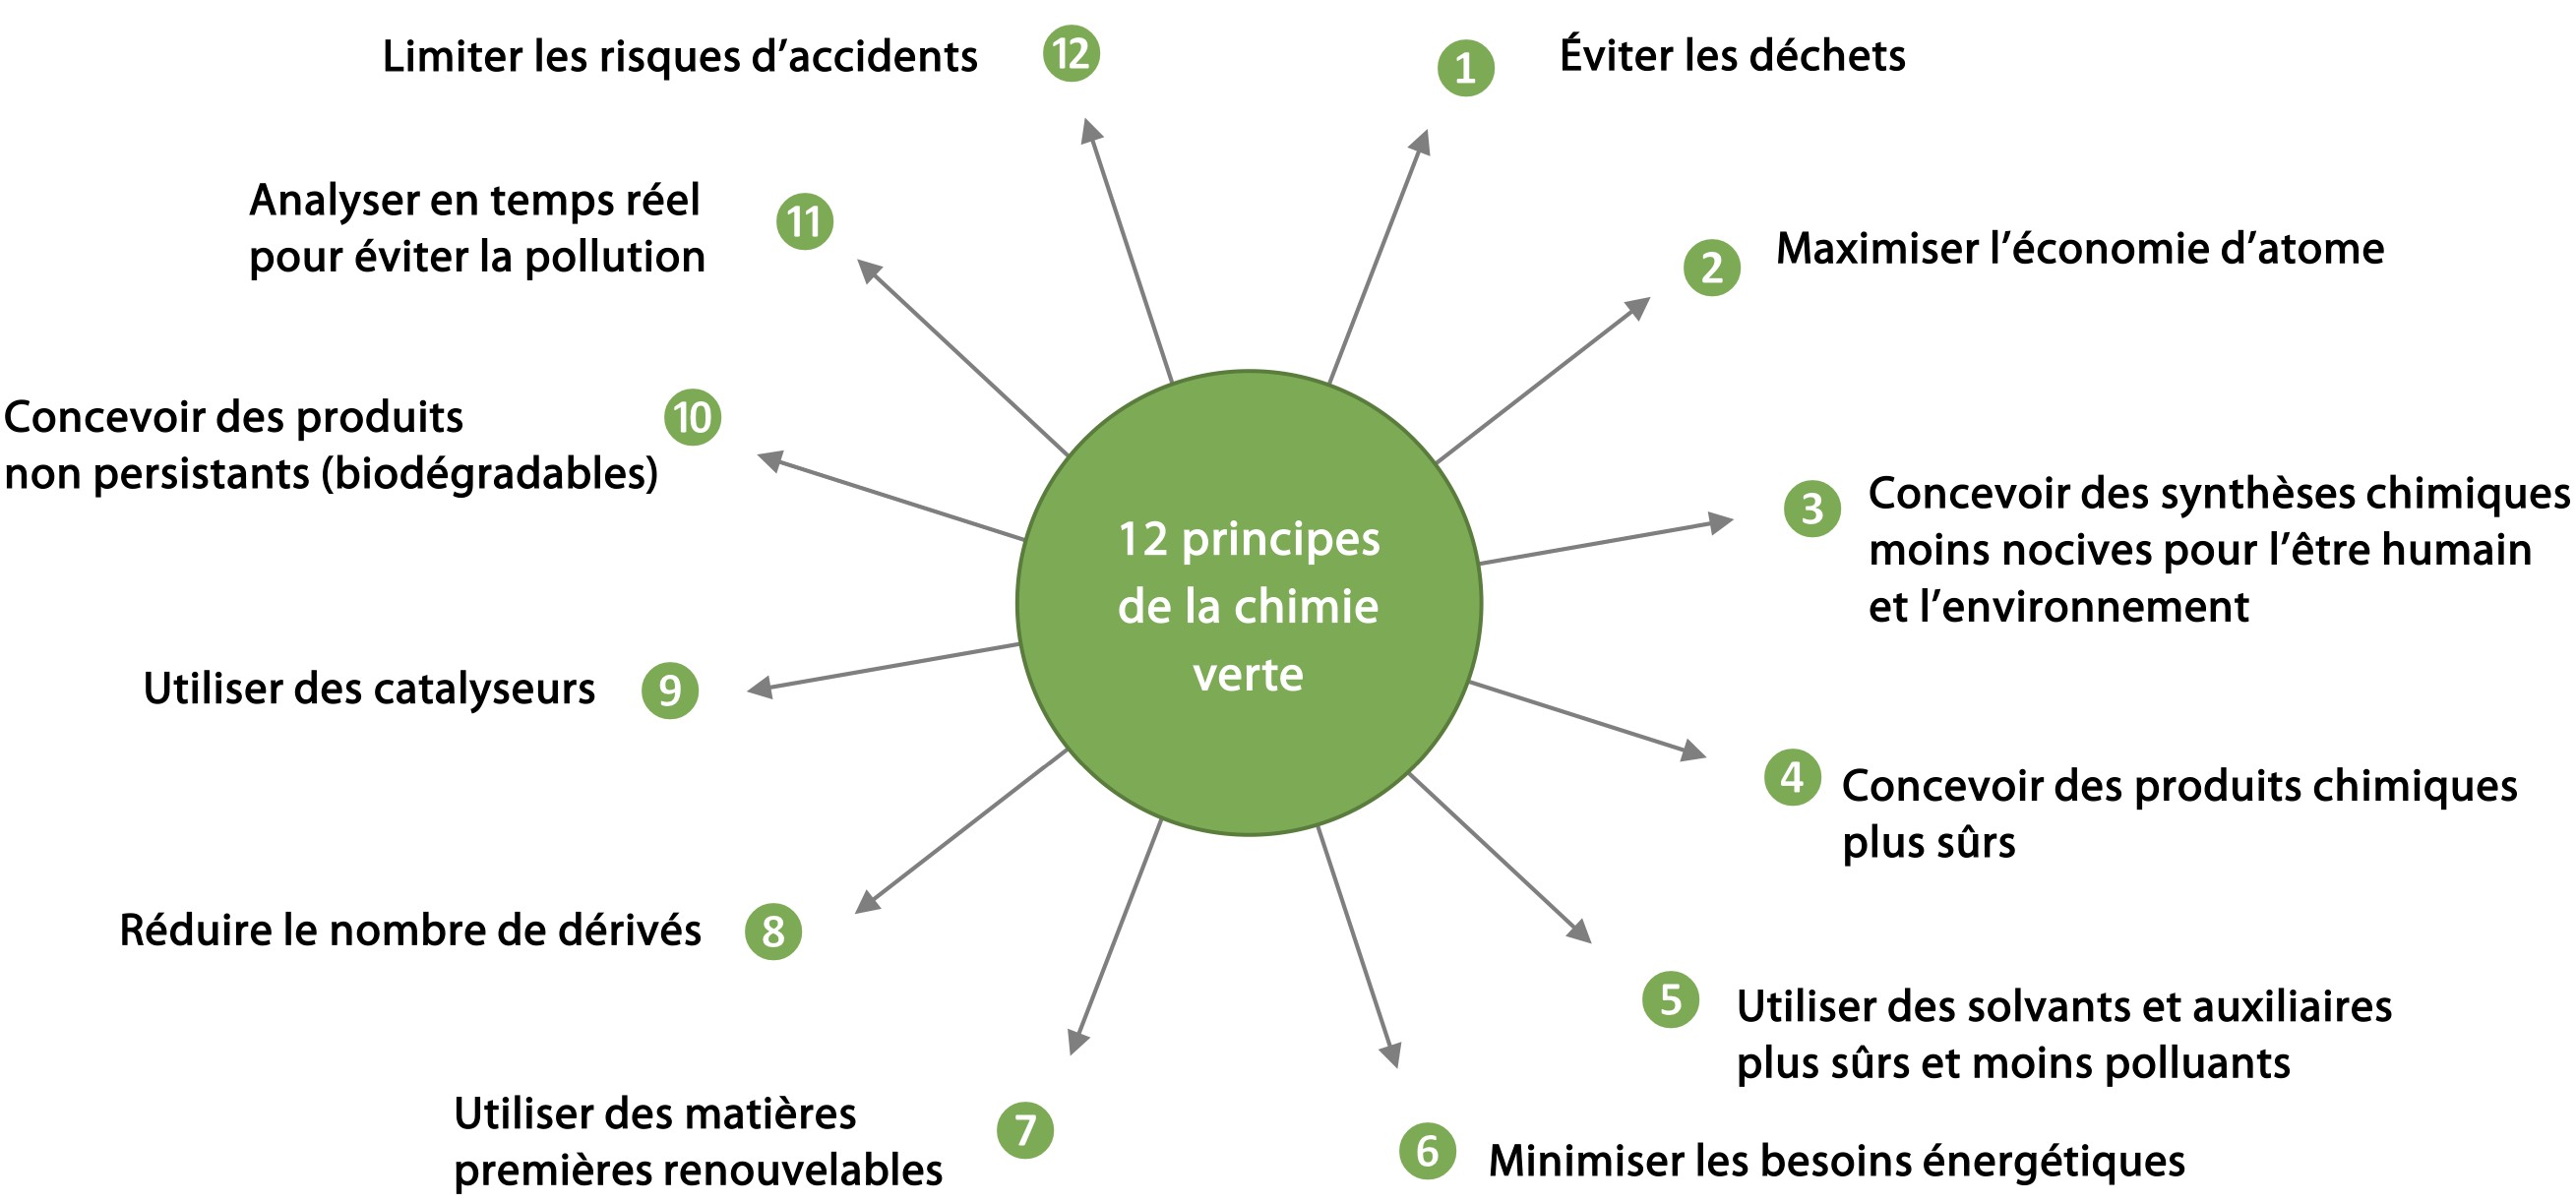
\includegraphics[width=.95\textwidth]{figures/chimie_verte}

\begin{travail}
\begin{itemize}
	\item Formules semi-développées, topologiques: 4, 5 p 202
	\item Rendement: 32 p 210 -  Protection: 33 p 211 - Dean Stark: Préparation ECE p 211
		\item Type BAC: \url{https://www.labolycee.org/synthese-dun-arome-dorange} BAC 2022
	\item Type BAC: \url{https://www.labolycee.org/synthese-dun-arome} BAC 2021

\end{itemize}
\end{travail}

%\setcounter{chapter}{21}
\chapter{Synthèse Organique (partie 2)}
\section{Représentation des molécules}

\subsection{Rappels}
revoir la nomenclature: savoir nommer une chaîne carbonée, identifier groupes caractéristiques et les familles organiques. 

\etiquette{Familles fonctionnelles}

\begin{center}
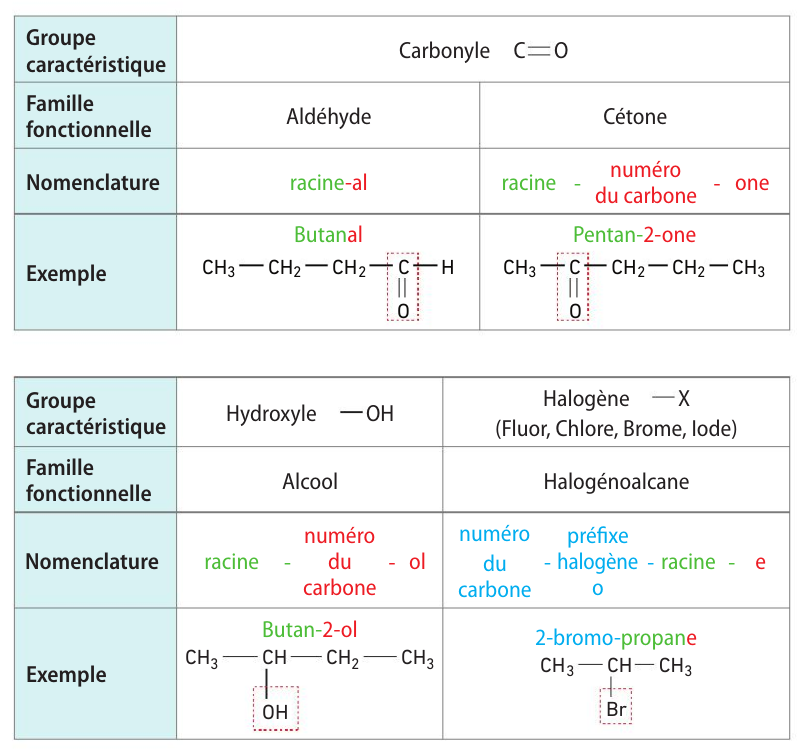
\includegraphics[scale=0.45]{figures/orga/fig_famille_1}\\
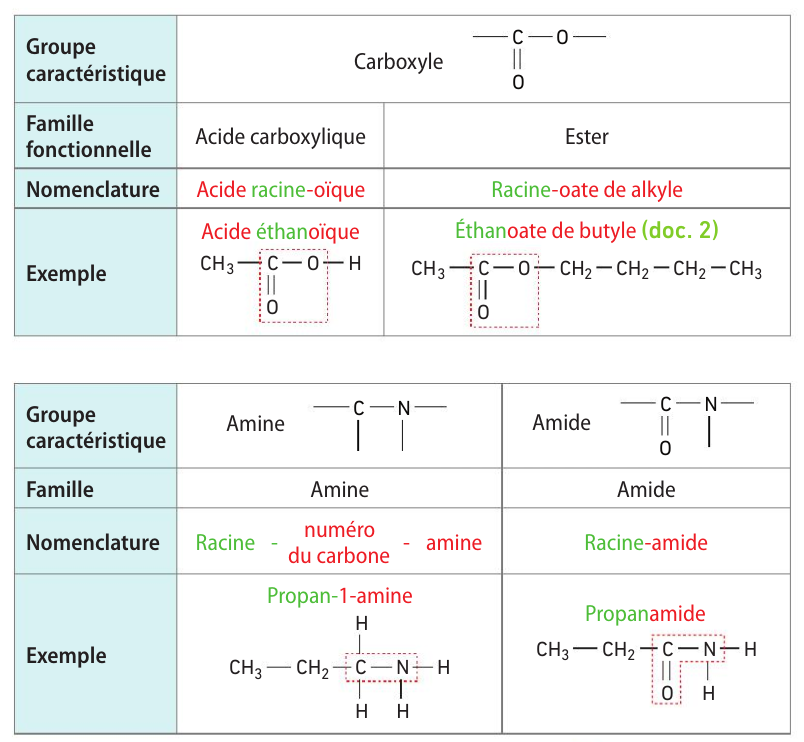
\includegraphics[scale=0.45]{figures/orga/fig_famille_2}
\end{center}

\section{L'isomérie de constitution}
\blocrouge{Définition}{
Deux espèces sont des isomères de constitution si \trou{elles ont la même formule brute mais des formules développées, semi-développées, topologiques différentes.}
}

Des isomères de constitution présentent souvent des propriétés physiques et chimiques \trou{différentes}.

\blocgris{Application}{
Trouver 2 isomères de l'espèce chimique ayant pour formule brute : $C_3H_6O_2$.
}

\section{Les polymères}
\blocrouge{Définition}{
Un polymère est une macromolécule, constituée d'un enchaînement répété d'un même motif, appelé \trou{monomère}, reliés les uns aux autres par des liaisons covalentes.
}

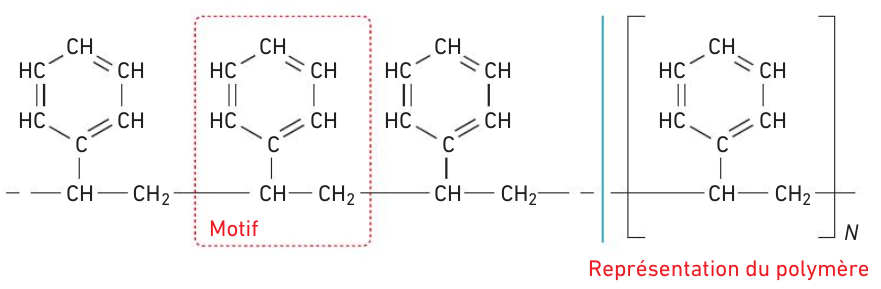
\includegraphics[scale=0.5]{figures/orga/fig_polymere}\\
On représente le polymère en écrivant le monomère entre crochets, avec le nombre de répétitions en indice.\\
Dans cette exemple, le monomère s'appelle le styrène, et le polymère le polystyrène.\\

\etiquette{Culture (au programme)} Les polymères peuvent être d'origine synthétique ou naturelle.\\
Par exemple, la cellulose que l'on trouve dans les mouchoirs en papier, ou le cis-polyisopropène que l'on trouve dans le latex sont d'origine naturelle.\\
Le polychlorure de vinyle ou PVC, que l'on trouve dans les revêtements de sol, les canalisations etc... est d'origine synthétique.



\section{La synthèse organique : optimisation de la vitesse et du rendement}
\subsection{Augmenter la vitesse d'une synthèse organique}

\begin{minipage}{0,7\linewidth}

Pour augmenter la vitesse de formation d'un produit, on peut :
\begin{itemize}
\item \trou{\textbf{Chauffer le milieu réactionnel} avec un montage à reflux pour éviter les pertes.}
\item \trou{\textbf{Augmenter la concentration} des réactifs en solution.}
\item \trou{ \textbf{Utiliser un catalyseur}. Le catalyseur est introduit en petite quantité dans le mélange réactionnel et il n'est pas consommé lors de la synthèse.}
\end{itemize}
Sur l'exemple ci-contre, on remarque que l'état final est le même, la quantité d'ester obtenue ne change pas, mais on atteint cet état final plus rapidement à 
$\SI{70}{\celsius}$ et encore plus rapidement si il y a un catalyseur.
\end{minipage}
\begin{minipage}{0,3\linewidth}

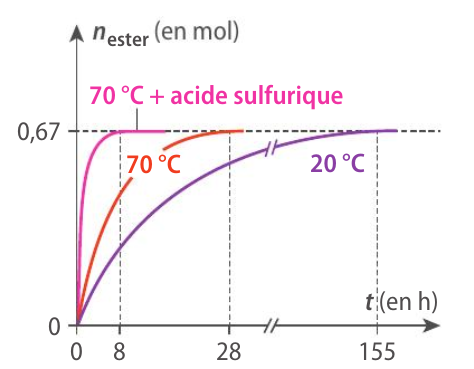
\includegraphics[scale=0.4]{figures/orga/fig_cinetique}
\end{minipage}
\subsection{Augmenter le rendement d'une synthèse organique}

\blocrouge{Définition}{
Le rendement d'une synthèse est \trou{le rapport entre la quantité de matière de produit  \trou{obtenu} et la quantité de matière théorique que l'on pourrait obtenir si la transformation chimique était \trou{totale} et qu'il n'y avait aucune perte.}
On le note : 
$$\eta=\dfrac{n_f}{n_{max}}=\dfrac{m_f}{m_{max}}$$ 
}

\subsection*{Constatations expérimentales}
On considère la réaction d'estérification, lors de laquelle un alcool réagit avec un acide pour donner un ester et de l'eau.\\
La réaction étudiée fait réagir l'éthanol et l'acide éthanoïque. L'ester obtenu est l'éthanoate d'éthyle.\\
La réaction s'écrit : 

$$CH_3CH_2-OH + CH_3-COOH\leftrightharpoons H-OH +CH_3COO-CH_2CH_3$$
$$\text{alcool} + \text{acide carboxylique}  \leftrightharpoons \text{eau}  + \text{ester}$$
On effecture 3 fois cette réaction pour des mélanges initiaux de réactifs différents. Les résultats obtenus sont:
\begin{center}
\begin{tabular}{l|cc||cc}
  & Etat Initial & (en mol) & Etat Final& (en mol)\\ \hline
  &$n_i(alcool)$ &$n_i(acide)$ &$n_f(ester)$&$n_f(eau)$\\
  \hline
 Cas n°1 &1,0&1,0&0,67&0,67 \\
 \hline
  Cas n 2 &1,0&5,0&0,946&0,946 \\
  \hline
  Cas n 3 &1,0&2,0&0,848&0,848 
\end{tabular}
\end{center}

\etiquette{Questions}
\begin{enumerate}
\item Quel est le réactif limitant dans chacun des cas ? Quelle est sa quantité de matière ?\\
\trou{Le réactif limitant est l'alcool dans chaque cas, et sa quantité de matière est égale à 1,0 mol.}
\item Calculer le rendement de la synthèse de l'ester dans chacun des cas.\\
\trou{Dans le cas 1, c'est 0,67\\
Dans le cas 2, c'est 0,94 et dans le cas 3, c'est 0,84}
\item Comparer l'évolution du rendement à l'évolution de la quantité de matière du réactif non limitant en fonction des différents cas. Que pouvez-vous conclure ?\\
\trou{On observe que plus la quantité de matière du réactif non limitant est importante, plus le rendement est élevé}
\item Cette observation est-elle en accord avec vos connaissances sur l'équilibre dynamique au niveau microscopique ?\\
\trou{En augmentant la quantité de matière de l'un des réactifs, la probabilité d'avoir des chocs efficaces entre les molécules de réactifs augmente, et donc $\tau_f$ augmente également}
\item En réfléchissant à l'équilibre dynamique au niveau microscopique, donner une autre idée qui permettrait d'augmenter le rendement de la synthèse.\\
\trou{En éliminant l'eau, cela évite que la transformation se fasse dans le sens indirect, et donc, cela augmente le rendement de la synthèse de l'ester}
\end{enumerate}

\blocrouge{Conclusion}{
Le rendement d'une synthèse augmente quand :
\vspace{0.3em}

\begin{itemize}
\item \trou{On introduit l'un des réactifs en excès}
\item \trou{On élimine du milieu réactionnel l'un des produits de la réaction.}
\end{itemize}
}



\etiquette{Exercices}
\begin{itemize}
	\item 10, 13 p 203
	\item 20, 21 p 204 
\end{itemize}

\etiquette{BAC}
\begin{itemize}
	\item \url{https://labolycee.org/optimisation-de-la-synthese-de-lethanoate-de-benzyle} : proche du cours
	\item \url{https://labolycee.org/larome-dananas} : Très complet
	\item \url{https://labolycee.org/le-nylon} : Polymère
\end{itemize}
 
\end{document}
